%!TEX TS-program = ./custom_compile.py

%! iTeXMac(project): POH.pTeXMac
%% Multi-part RV-8 POH, created by Kevin Horton
%% This is the master file, which includes the files for each section

%% To get pdf output: 
%% latex POH.tex
%% dvips -t letter -o POH.ps POH.dvi
%% ps2pdf POH.ps POH.pdf

%% To Print
%% Open in Adobe Acrobat Reader v7.0.5
%% Select landscape orientation in Page Setup
%% In the Print dialog box, select Odd Pages, Page Scaling - None, and deselect Auto-Rotate 
%% and Center.  This will put the odd pages on the left side of the page.  Print the odd pages.
%% Take the output, put it in the input tray, with the printed side up, and the printed end away 
%% from the printer (i.e. the blank portion goes in the printer first).  Select Even Pages Only, 
%% and print.

%% Using latex then dvipdf puts the pages too high, so the header is off the top of the page.  
%% Using pdflatex causes problems with many "non-pdf special ignored", as some of the 
% % packages used are not compatible with pdflatex.  This results in some of the lines 
%% in figures not drawn being drawn.

% % If latex is used, the graphics files must be .eps files.  If starting with a pdf graphics file, care
% % must be taken to ensure the conversion to .eps uses vector fonts.  Using ghostscript seems 
% % to often result in bitmap fonts, possibly because TrueType fonts were used in the original
% % pdf, rather than Type 1 fonts.

% % To get eps graphics files from pdf files, with vector fonts, use pdftops -eps (part of xpdf 
% % package).  The bounding box in resulting .eps file may be manually editted to get the 
% % display correct, or a "bb= " statement can be put in the latex code that adds the graphic.

%% Custom typeset scritp in iTexMac is "latex ${iTMInput}; dvips -t letter -o ${iTMInput}.ps ${iTMInput}.dvi;ps2pdf ${iTMInput}.ps ${iTMInput}.pdf; open ${iTMInput}.pdf"

%% Chapter vs Sections - each major division in the POH is labeled as a "Section" in the
%% printed output.  However, these divisions are called "Chapters" in LaTeX.  Thus each
%% major division is labeled with \chapter, and the next division lower in the hierarchy is labeled
%% \section.  It was deemed to be easier to do it this way than to do a major rework of the class
%% and package files.

% FOR FINAL PRINT!!
% Add the aircraft registration in the page header, and remove the date in the page footer, 
% see the scrpage2 portion of this file. 

% TO DO
% Trial picins package vice wrapfig to better handle figures in the vicinty of lists.
% Are kg values really required?  Review AMA 549.  Review indicates kg values are probably only needed for placards.
% Figure out how to reduce space after "NOTES" and the items when enumerate is used.
% Intro - review General section.  Should there be more info here?
% Intro - review Oil section against Lycoming Operator's Manual.  Should the "Ashless Dispersant Grades" text be in the right column?
% emer.tex - write missing emer sections
% emer - rework to match checklist
% emer - static source blockage.
% emer - icing encounter?
% emer - speeds for emergency operation - add code to adjust weight for VA
% emer checklist - checked against C177 to Static source blockage (following C177 order)
% TOC.  Use tocloft to get "SECTION" over top of the list of chapter numbers.  See page 7-8 of tocloft.pdf.
% Section TOCs - sort out how to handle Figure lines
% Why is the List of Figures blank? - LOF  removed for now, perhaps it isn't needed.
% Normal - finish Amplified Procedures
% W&B chapter - complete
% Perf chapter - complete.  Revise charts to have 1900 lb and 1800 lb numbers?
% Perf - review mixture setting info from Mooney and Beech POHs - full rich at high power, or set specified fuel flow?  See Cruise Power chart, 
% Perf - figure out how to make all wide charts the same width, and how to get mixture setting charts lined up on RH side.
% Systems - sort out Overfull \hbox on Stick Grip diagram.
% Systems - get up to date GNS 430W display picture
% Systems - Get up-to-date panel diagram, with compass above glareshield
% Systems - Add info on annunciator light  and trim indicator dimmer.
% Systems - Check whether flux valve ON/OFF is discussed.
% Service chapter - complete
% look at format for small page size, suitable for cockpit carriage.
% tweak float placement parametres to get perf figures at the top of pages. It seems like they are on float pages, and they are centered vertically.
% Add 3-View with dimensions on page 4
% Use \minisec where required to have an unnumbered heading close to following text.  See scrguien.pdf pg 73

% REVIEW AT END
%
% Review quote symbols.  Need double ` for left quote, and double ' for right quote.   OK as of 19 Oct 04.
% Put section names in uppercase, subsection in Capitalize Words.  OK as of 23 Oct 04.
% Fonts - Use Times?  See psnfss2e.pdf - Seems to work OK - try a comparitive printout.
% Review page breaks, after all editing is complete.  Use \addpenalty as required to suggest better places for page breaks.
% % \\* prohibits a page break after a forced line break.
% % \mbox{text} forces all of "text" to be on one line.
% % ~ is a space that cannot be enlarged, or be at a line break.
% degree symbols - consider replacing \textdegree with $\30,^{\circ}\mathrm{C}$.  See lshort.pdf
% PDF file - consider use of pdflatex, to get hyperlinks in index, etc.  Use epstopdf to convert all .eps files to .pdfs. See lshort.pdf pg 73.  Use hyperfef package.

% to create PDF file from GSView on Windows - open file in GSView.  Media, Letter.  File, Convert.  Select pdfwrite.  Select Properties.  Use X offset of 0, and Y offset of -45. 

% to extract text, run "ps2ascii POH.pdf POH.txt"

\documentclass[twoside,titlepage,chapterprefix,10pt]{scrbook}
% \documentclass[twocolumn,titlepage,chapterprefix,10pt]{scrbook}

%%
%% go back to T1 fontenc, once the CM super font package is installed
%%\usepackage[T1]{fontenc}
\usepackage[OT1]{fontenc}
\usepackage[latin1]{inputenc}
\setcounter{secnumdepth}{0} % was 3
\setlength{\parskip}{\medskipamount}
\setlength{\parindent}{0pt}
\usepackage{array}% removed to try the tabls package instead (see TLC2 pg 269)
\usepackage{boxedminipage} % to put frame around graphs in performance section
\usepackage{calc}
%\usepackage{caption}
\usepackage{chappg} % to get page numbers like 3-5
\usepackage[strict]{chngpage}% used to set smaller margins for checklists
\usepackage{color}
\usepackage{datetime}% used to get date format like 04 Jun 2004.
  \newdateformat{cdndate}{\twodigit{\THEDAY} \ \shortmonthname \ \THEYEAR}
%\usepackage{fancyhdr}
%%  \fancyhead[LE,RO]{\slshape \rightmark}
%  \fancyhead[LE,RO]{\slshape \leftmark}
%  \fancyhead[LO,RE]{\slshape RV-8 C-XXXX}
%%  \fancyhead[LO,RE]{\slshape RV-8 C-GNHK}
%  \fancyfoot[C]{\thepage}
%  \fancyfoot[LE,RO]{\scriptsize\today} % remove this for the final printing
%  \pagestyle{fancy}
\usepackage{flafter}  % keep floats from coming before the reference
% \usepackage{floatflt} % to wrap text around figures
% \usepackage[paper=a4paper,landscape=true]{geometry}
%\usepackage[paper=a4paper]{geometry}
\usepackage[paper=letterpaper]{geometry}
  \newlength{\maintopmargin} % top margin for main part of POH
  \newlength{\mainbottommargin} % bottom margin for main part of POH
  \newlength{\maininnermargin} % inner margin for main part of POH
  \newlength{\mainoutermargin} % outer margin for main part of POH
%  \setlength{\maintopmargin}{0.5in}
  \setlength{\maintopmargin}{0.75in}
  \setlength{\mainbottommargin}{.75in}
  \setlength{\maininnermargin}{1in}
  \setlength{\mainoutermargin}{1in}
%  \newlength{\checklisttopmargin} % top margin for checklists
%  \newlength{\checklistbottommargin} % bottom margin for checklists
%  \newlength{\checklistinnermargin} % inner margin for checklists
%  \newlength{\checklistoutermargin} % outer margin for checklists
%  \setlength{\checklisttopmargin}{0.1in}
%  \setlength{\checklistbottommargin}{0.1in}
%  \setlength{\checklistinnermargin}{0.1in}
%  \setlength{\checklistoutermargin}{0.1in}
%  \geometry{verbose,letterpaper,tmargin=0.5in,bmargin=1in,lmargin=1in,rmargin=0.5in}


\geometry{verbose,letterpaper,tmargin=\maintopmargin,bmargin=\mainbottommargin,inner=\maininnermargin,outer=\mainoutermargin}
% \geometry{verbose,a4paper,tmargin=\maintopmargin,bmargin=\mainbottommargin,inner=\maininnermargin,outer=\mainoutermargin}


\usepackage{graphicx}
%\usepackage{layout}
% \usepackage{layouts}
%   \newcommand\showpage{%
%     \setlayoutscale{0.27}\setlabelfont{\tiny}%
%     \printheadingsfalse\printparametersfalse
%     \currentpage\pagedesign}
\usepackage{longtable} % for EIS page format table
\usepackage{mdwlist}
\usepackage{minitoc}
%  \setcounter{parttocdepth}{0}
  \setcounter{minitocdepth}{3}
%  \setcounter{minilofdepth}{2} % not defined
  \renewcommand{\mtcSfont}{\bf}
  \renewcommand{\mtctitle}{TABLE OF CONTENTS}
  \renewcommand{\mtifont}{\Large \sffamily \bfseries}  
  \renewcommand{\mtcfont}{\rm}
  \renewcommand{\mlffont}{\bf}
  \renewcommand{\mlftitle}{LIST OF FIGURES}
%  \renewcommand{\mlffont}{\Large \sffamily \bfseries}  
  \renewcommand{\mlffont}{\rm}
  
  \newlength{\minitocspacebefore} % define vertical space between chapter name and minitoc
  \setlength{\minitocspacebefore}{10ex}
\usepackage{multicol}
\usepackage{multirow} % used in performance tables
\usepackage{overpic} % to overlay text on graphics.  Used for side view in W&B section
%\usepackage{paralist} % to get compact description environment
%\usepackage{pdfsync} % to get back and forth syncing between TextMate and Skim
\usepackage{picins}
\usepackage{pict2e} % to get arrows in stick grip figure
\usepackage{pifont} % to get Zapf Dingbats
\usepackage{placeins} % to get FloatBarrior, to force figures before next section
%\usepackage{pspicture} % to get arrows in stick grip figure - superceded by pict2e package
%\usepackage{pstricks} % to get white circles for background for numbers in autopilot graphic
\usepackage{ragged2e} % to get the justifying option to make NOTES
\usepackage[figuresright]{rotating} % needed for Takeoff Perf table
\usepackage{scrpage2} % KOMA-Script heading package
  \pagestyle{scrheadings}
  \ihead{RV-8 C-GNHK} % put aircraft ID in the inner header
  \ohead{\leftmark} % put Section name in outer header
  % \ifoot{DRAFT --- \thistime \ \cdndate\today} % replace with issue date eventually
  \ifoot{Created --- \thistime \ \cdndate\today} % replace with issue date eventually
\usepackage{scrtime} % needed to get the \thistime command for the footer.  Not needed for the final document.  
\usepackage[pageshow]{supertabular} % for long table of EIS page formats, but it puts whole table on one page :(
%\usepackage{tabls} %conflicts with array package
\usepackage{tabularx}
  \newcolumntype{Y}{>{\raggedright\arraybackslash}X}
\usepackage{textcomp} % for to get degree symbols from \textdegree
\usepackage{titletoc}% allows formatting TOC without page numbers, and custom format to get chapter number at right
  \titlecontents{chapter}[0pc]{\vspace{5ex} \bfseries \sffamily \large}{}{\contentslabel[\chaptername]{0pc}}{\dotfill SECTION \thecontentslabel}
  \renewcommand\contentsname{TABLE OF CONTENTS}
\usepackage{wrapfig} % wrap text around small figures

\usepackage{stmaryrd} % for boxes

% Following packages change the default fonts to Times and Helvetica
\usepackage{mathptmx}
\usepackage[scaled=.92]{helvet}
\usepackage[T1]{fontenc}
\usepackage{textcomp} 
\usepackage[ps2pdf,bookmarks=true]{hyperref}
\hypersetup{
pdfauthor = {Kevin Horton},
pdftitle = {POH},
pdfsubject = {Pilot's Operating Manual --- RV-8 C-GNHK},
%pdfkeywords = {Keyword1, Keyword2, ...},
pdfcreator = {LaTeX with hyperref package},
pdfproducer = {dvips + ps2pdf}}

%\addtokomafont{sectioning}{\MakeUppercase}% change section names to upper case - doesn't work

\makeatletter
%%%%%%%%%%%%%%%%%%%%%%%%%%%%%% LyX specific LaTeX commands.
\newcommand{\lyxline}[1]{
  {#1 \vspace{1ex} \hrule width \columnwidth \vspace{1ex}}
}
%% Bold symbol macro for standard LaTeX users
\newcommand{\boldsymbol}[1]{\mbox{\boldmath $#1$}}
%% Because html converters don't know tabularnewline
\providecommand{\tabularnewline}{\\}
\makeatother


%\includeonly{intro,limitations,emer_checklist,emer,normal,normal_checklist,systems}

%% following five commands to control the placement of figures on the pages.
\renewcommand{\textfraction}{0.10} % default is 0.2, or minimum 20% of page for text.
\renewcommand{\topfraction}{0.9} % default is 0.7, or maximum of 70% at top of page for a figure.
\renewcommand{\bottomfraction}{0.9} % default is 0.3, or maximum of 30% at bottom of page for a figure.
\renewcommand{\floatpagefraction}{0.35} % default is 0.5, or minimum 50% of a page covered by figures without any text.
%\setcounter{totalnumber}{5} % default is maximum of 3 figures per page.

%% force "This Page Intentionally Blank" on blank pages
\makeatletter 
\def\cleardoublepage{\clearpage\if@twoside \ifodd\c@page\else 
  \hbox{} 
  \vspace*{\fill} 
  \begin{center} 
    \Large  THIS PAGE INTENTIONALLY LEFT BLANK.
  \end{center} 
  \vspace{\fill} 
  \thispagestyle{empty} 
  \newpage 
  \if@twocolumn\hbox{}\newpage\fi\fi\fi} 
\makeatother 

%% Multi-line description labels - TLC2, pg 148 & 150
\usepackage{calc}
\newenvironment{Description}
   {\begin{list}{}{\let\makelabel\Descriptionlabel
%      \setlength\labelwidth{120pt}%
      \setlength\labelwidth{110pt}%
      \setlength\leftmargin{\labelwidth+\labelsep}}}%
   {\end{list}}
\newcommand*\Descriptionlabel[1]
   {\raisebox{0pt}[1ex][0pt]%
      {\makebox[\labelwidth][l]%
         {\parbox[t]{\labelwidth}%
%                    {\hspace{0pt}\textsf{#1:}}}}}
                    {\hspace{0pt}\textrm{#1}}}}}
                    
%% New environment for perf chart headers
\newenvironment{perfhdr}
  {\sffamily\huge\begin{center}}
  {\end{center}\vspace{5ex}\normalfont\normalsize}
  
% New space used to set height between Notes and charts in perf section
\newlength{\perfnoteskip}
\setlength{\perfnoteskip}{5ex}
  
%% New environment for NOTES, CAUTIONS and WARNINGS
\newcounter{oldparindent}
\newenvironment{Note}[1][NOTE]
  {
    \setcounter{oldparindent}{\parindent} 
    \begin{quote}
    \centering{\textbf{#1}}
    \\ 
    \justifying  
    \parindent=0pt
  }
  {
    \parindent \value{oldparindent}pt
    \end{quote}
  }

%% New environment for NOTES, CAUTIONS and WARNINGS in checklists
%% Same as normal notes, but no indent.
\newenvironment{Note2}[1][NOTE]
  {
    \setcounter{oldparindent}{\parindent} 
    \centering{\textbf{#1}}
    \\ 
    \justifying  
    \parindent=0pt
  }
  {
    \parindent \value{oldparindent}pt
  }

%% New environment for NOTES, CAUTIONS and WARNINGS
%% Same as normal notes, but with the note text centered, useful for one line notes
\newenvironment{NoteCtr}[1][NOTE]
  {
    \setcounter{oldparindent}{\parindent} 
    \begin{quote}
    \centering{\textbf{#1}}
    \\ 
    \parindent=0pt
  }
  {
    \parindent \value{oldparindent}pt
    \end{quote}
  }



\renewcommand\chaptername{SECTION} % used to have "SECTON" appear on the first page of every chapter

%% get thicker horizontal rule for tables.  From TLC2, pg 266
\newlength{\savedwidth}
\newcommand\whline{\noalign{\global\savedwidth\arrayrulewidth
                                                 \global\arrayrulewidth 1pt}%
                                                 \hline
                                                 \noalign{\global\arrayrulewidth\savedwidth}}

% following lengths are used to set row widths to fit the text
\newlength{\colOne}
\newlength{\colTwo}
\newlength{\colThree}
\newlength{\colFour}
\newlength{\colFive}
\newlength{\colSix}
\newlength{\colSeven}
\newlength{\colEight}
\newlength{\rowdrop}
\setlength{\rowdrop}{\baselineskip/-1}
% halfrowdrop is equal to one half the normal line spacing.  It is used to drop table headers one-half row, as required to good alignment.
\newlength{\halfrowdrop}
\setlength{\halfrowdrop}{\baselineskip/-2}

\newlength{\olditemident}% used when adjusting ident for list environments

\newenvironment{checklist}
  {
  % \changepage{textheight}{textwidth}{evensidemargin}{oddsidemargin}{columnsep}{topmargin}{headheight}{headsep}{footskip}
%  \changepage{74pt}{130pt}{-65pt}{-65pt}{}{-28pt}{0pt}{0pt}{0pt}% original settings, with no room for header or footer, 0.5 top margin, 0.75 bottom margin, 1 in left and right margins
  \changepage{56pt}{130pt}{-65pt}{-65pt}{}{-46pt}{0pt}{0pt}{0pt}% original settings, with no room for header or footer
%  \changepage{59pt}{130pt}{-65pt}{-65pt}{}{-3pt}{0pt}{-10pt}{0pt}% revised settings, with room for header
  }
  {
  \cleardoublepage
  Bogus page
  \cleardoublepage
  \changepage{-56pt}{-130pt}{65pt}{65pt}{}{46pt}{0pt}{0pt}{0pt}% original settings, with no room for header or footer
  }
  
% Checklist - parametres to change page margins
\newlength{\checklistTextHeight}
\newlength{\checklistTextWidth}
\newlength{\checklistEvenSideMargin}
\newlength{\checklistOddSideMargin}
\newlength{\checklistTopMargin}
\setlength{\checklistTextHeight}{56pt}
\setlength{\checklistTextWidth}{130pt}
\setlength{\checklistEvenSideMargin}{-65pt}
\setlength{\checklistOddSideMargin}{-65pt}
%\setlength\checklistTopMargin{-46pt} % no room for header, but room for footer
\setlength{\checklistTopMargin}{-12pt} % room for header, but not footer

% set thickness of vertical rules for multitcolumns in checklists
\setlength{\columnseprule}{0.4pt}

% Define Direct-To symbol to look like marking on that key on the GNS 430
\def\directto{${\mkern6mu D\mkern-24mu \longrightarrow \mkern2mu}$} 

% allow different POH for different declared max takeoff weight
\newcounter{MTOW} % maximum takeoff weight in lbs
  \setcounter{MTOW}{1900}
\newcounter{MTOWkg} % MTOW in kg
  \setcounter{MTOWkg}{\value{MTOW}/\real{2.2046}}
\newcounter{MTOWkgdecimal}
  \setcounter{MTOWkgdecimal}{\value{MTOW}/\real{.22046}-(\value{MTOWkg}*10)}

%%%%%%%%%%%%%%%%%%%%%%%%%%%%%% Start of Document
\begin{document}
%\showpage causes the page layout to be drawn in the resulting dvi or pdf file.  Defined in preamble.
% \showpage
\setlength{\extrarowheight}{1.5pt} % needs array package
\dominitoc % can remove, if minitoc package is no longer used
% \dominilof % can remove, if minitoc package is no longer used
\frontmatter
% !iTeXMac(input): POH.tex
\title{Pilot's Operating Handbook\\
[1in]RV-8 C-GNHK\\
[0.25in]Ser. No. 80427}

\author{Kevin Horton}


\date{13 Aug 2021}


\maketitle \clearpage

%\vfill
%\centering Typeset with \LaTeXe
%\vfill
\cleardoublepage \setcounter{tocdepth}{0} 

% only need chapter names in main TOC
%\newsavebox{\TOCtitle}
%\sbox{\TOCtitle}{\bfseries \sffamily \Huge TABLE OF CONTENTS \textnormal}
%\centering \usebox{\TOCtitle}
\tableofcontents{}

%\listoffigures{}
\clearpage

%\listoffigures
%%\clearpage
%\cleardoublepage
%\vfill
\mainmatter

%\layout % show page layout. Needs layout package.
%\pagediagram % show page layout. Needs layouts package.
%% Following three lines show a minipage diagram, with margins shown
%\currentpage
%\setlayoutscale{0.5}
%\pagedesign
%\setcounter{chapter}{1}
\chapter{GENERAL} \vspace{\minitocspacebefore} \minitoc \clearpage

% 3-view
%\addcontentsline{toc}{section}{\numberline{}THREE-VIEW}
\addcontentsline{toc}{section}{THREE-VIEW}

\begin{figure}
	\begin{center}
		
		\begin{overpic}
			% The following command works with the pspicture package
			% {../Diagrams/3-view/3view} \put(47.2,13){\Line(0,11)} \put(0.6,13){\Line(0,11)} \put(23.25,23){23'} \arrowlength{4pt} \put(22.5,23.4){\Vector(-21.9,0)} \put(25.3,23.4){\Vector(21.9,0)} \put(44,79.4){\Line(5,0)} \put(42,91.8){\Line(7,0)} \put(47,85){\textcolor{red}{5' 7''}} \put(48.3,84.5){\Vector(0,-5.1)} \put(48.3,86.7){\Vector(0,5.1)} \put(45.4,79.5){\Line(0,-2.8)} \put(3.2,89){\Line(0,-12.2)} \put(23.4,77){\textcolor{red}{21'}} \put(22.65,77.4){\Vector(-19.45,0)} \put(25.95,77.4){\Vector(19.45,0)} 
			% The following command works with the pict2e package
			{../Diagrams/3-view/3view} \put(47.2,13){\line(0,1){11}} \put(0.6,13){\line(0,1){11}} \put(23.25,23){23'} \put(22.5,23.4){\vector(-1,0){22}} \put(25.3,23.4){\vector(1,0){22}} \put(49,79.4){\line(-1,0){50.4}} \put(42,91.8){\line(1,0){7}} \put(47,85){5' 10''} \put(48.3,84.5){\vector(0,-1){5.1}} \put(48.3,86.7){\vector(0,1){5.1}} \put(45.4,79.5){\line(0,-1){2.8}} \put(3.2,89){\line(0,-1){12.2}} \put(23.4,77){21'} \put(22.65,77.4){\vector(-1,0){19.45}} \put(25.95,77.4){\vector(1,0){19.45}} \put(-1.4,95.5){\line(1,0){7}} \put(-2,86.85){7' 10''} \put(-0.7,86.35){\vector(0,-1){6.95}} \put(-0.7,88.55){\vector(0,1){6.95}} 
		\end{overpic}
	\end{center}
	\caption{Three View} 
\end{figure}

\clearpage 
\section{INTRODUCTION} This Pilot's Operating Handbook contains nine sections with all the information required to operate the aircraft. 

\textcolor{red}{Items in red text are preliminary, and are subject to change pending the results of ground and flight tests.}

Section 1 provides basic data and information of general interest. It contains definitions or explanations of abbreviations and terminology commonly used.

This aircraft is certificated in the Amateur-Built category. The regulations governing the Amateur-Built category contain only very limited performance requirements, and no flight characteristics requirements. By virtue of its amateur-built status, all persons entering this aircraft do so at their own risk.

\section{DESCRIPTIVE DATA} 
\subsection{ENGINE} 
\begin{Description}
	\item[Engine Manufacturer:] Lycoming 
	\item[Engine Assembler:] Aerosport Power, Kamloops, B.C. 
	\item[Engine Model Number:] IO-360-A1B6 
	\item[Engine Type:] Four cylinder, Direct Drive Horizontally Opposed, Air-Cooled, Fuel-Injected
	\item[Horsepower Rating:] 200 BHP 
	\item[Maximum Engine Speed:]2700 RPM 
	\item[Displacement:] 361 $\mathrm{in^{3}}$ 
	\item[Compression Ratio:] 8.7:1 
	\item[Time Between Overhaul:] 2000 hr 
\end{Description}

\subsection{PROPELLER} 
\begin{Description}
	\item[Manufacturer:] MT 
	\item[Model:] MTV-12-B-C/C183-59b 
	\item[Number of blades:] 3 wood core blades with stainless steel leading edges
	\item[Diameter:] 72.05 inches (183 cm)
	\item[Type:] Hydraulically Actuated Constant Speed 
        % TBO data from MT Service Bulletin No 1
	\item[Time Between Overhaul:] 1800 hr or 72 months 
\end{Description}

\subsection{FUEL} 
\begin{Description}
	\item[Total Fuel Capacity:] 163.5 l (43.2 USG) 
	\item[Usable Fuel Capacity:] 162.8 l (43 USG)
	\item[Approved Fuel Grades:] 100/130\\
	100 (Green)\\
	100LL (Blue) 
\end{Description}

\subsection{OIL} 
\begin{Description}
	\item[Oil Capacity:]8 US qts 
	\item[Specification:]Ref Lycoming Operator's Manual Pg 3-12B 
\end{Description}

% @{} at start of column spec used to supress space to the left of the tabular. See LaTeX Manual, pg 205-206.
\begin{tabular}
	{@{}lcc} Approved Grades& MIL-L-6082B& MIL-L-22851\tabularnewline & & Ashless Dispersant Grades\tabularnewline All Temperatures& --& SAE 15W50 or SAE 20W50\tabularnewline Above 27\textdegree C (80\textdegree F)& SAE 60& SAE 60\tabularnewline Above 16\textdegree C (60\textdegree F)& SAE 50& SAE 40 or 50\tabularnewline -1\textdegree C to 32\textdegree C (30\textdegree F to 90\textdegree F)& SAE 40& SAE 40\tabularnewline -18\textdegree C to 21\textdegree C (0\textdegree F to 70\textdegree F)& SAE 30& SAE 40, 30 or 20W40\tabularnewline Below -12\textdegree C (10\textdegree F)& SAE 20& SAE 30 or 20W30\tabularnewline 
\end{tabular}

\subsection{BRAKES}
\begin{Description}
	\item [Brake Fluid (preferred):]MIL-PRF-83282
	\item [Brake Fluid (acceptable):]MIL-H-5606.  Note: this fluid can be mixed with the preferred fluid, but has a much lower flash point so should be avoided if possible
\end{Description}

\subsection{MAXIMUM WEIGHTS} 
\begin{Description}
	
	%\item[Maximum Take-Off/\\Landing Weight:] 816.5 kg (1800 lb)\\
	%      \item[Max Take-Off Weight:] 1900 lb (861.8 kg)
	%      \item[Max Landing Weight:] 1900 lb (861.8 kg)
	
	\item[Max Take-Off Weight:] \theMTOW \space lb (\theMTOWkg .\theMTOWkgdecimal \space kg) 
	\item[Max Landing Weight:] \theMTOW \space lb (\theMTOWkg .\theMTOWkgdecimal \space kg) 
%	\item[Max Passenger Weight:] 300 lb (136.1 kg) (subject to Weight \& Balance) 
%	\item[Max Baggage Weight:] 125 lb (56.7 kg) (subject to Weight \& Balance) 
%	\item[Empty Weight :] 1194 lb (542 kg) (Incl full oil) - Weighed 27 Apr 2010, corrected for autopilot installation
	\item[Empty Weight :] 1182 lb (536 kg) (Incl full oil) - Weighed 27 Apr 2010, corrected on 26 No 2019 for ADS-B installation
	\item[Max Useful Load:] 718 lb (326 kg) (subject to Weight \& Balance) 
\end{Description}

\subsection{SPECIFIC LOADINGS} 
\begin{Description}
	\item[Wing Loading:]17.3 $\mathrm{lb/ft^{2}}$ 
	\item[Power Loading:]9.5 $\mathrm{lb/hp}$ 
\end{Description}

\section{NOTES, CAUTIONS AND WARNINGS} Specific items requiring emphasis are expanded upon and ranked in increasing order of importance in the form of a NOTE, CAUTION or WARNING.

\begin{Note}
  Expands on information which is considered essential to emphasize. Information contained in notes may also be safety related.
\end{Note}

\begin{NoteCtr}[CAUTION]
  Provides information that may result in damage to equipment if not followed.
  \end{NoteCtr}

\begin{NoteCtr}[WARNING]
  Emphasizes information that may result in personal injury or loss of life if not followed.
  \end{NoteCtr}


\section{TERMINOLOGY AND ABBREVIATIONS} 
\subsection{GENERAL AIRSPEED TERMINOLOGY} 
\begin{Description}
	\item[KIAS] \textbf{Knots Indicated Airspeed} is the speed shown on the airspeed indicator assuming no instrument error, expressed in knots.
	
	%   \item[KIAS] IAS in Knots.
	
	\item[KCAS] \textbf{Knots Calibrated Airspeed} is indicated airspeed corrected for position and instrument error, expressed in knots. Calibrated airspeed is equal to true airspeed in standard atmosphere at sea level.
	
	%    \item[KCAS] CAS in Knots.
	
	\item[KTAS] \textbf{Knots True Airspeed} is the airspeed relative to undisturbed air, expressed in knots, which is KCAS corrected for altitude, temperature and compressibility. 
	\item[GS] \textbf{Ground Speed} is the speed of the aircraft relative to the ground. 
	\item[$\mathrm{V_{A}}$] \textbf{Manoeuvring Speed} is the maximum speed at which abrupt full control deflection will not overstress the aircraft. 
	\item[$\mathrm{V_{FE}}$] \textbf{Maximum Flap Extension Speed} is the highest speed permissible with wing flaps in a prescribed extended position. 
	\item[$\mathrm{V_{NO}}$] \textbf{Maximum Structural Cruising Speed} is the speed that should not be exceeded except in smooth air, and then only with caution. 
	\item[$\mathrm{V_{NE}}$] \textbf{Never Exceed Speed} is the speed limit that may not be exceeded at any time. 
	\item[$\mathrm{V_{S}}$] \textbf{Stalling Speed} is the minimum steady flight speed at which the aircraft is controllable in a specified configuration. 
	\item[$\mathrm{V_{S_{0}}}$] \textbf{Stalling Speed in the landing configuration} at the most forward centre of gravity. 
	\item[$\mathrm{V_{X}}$] \textbf{Best Angle of Climb Speed} is the speed which results in the greatest altitude gain in a given horizontal distance. 
	\item[$\mathrm{V_{Y}}$] \textbf{Best Rate of Climb Speed} is the speed which results in the greatest altitude gain in a given time. 
\end{Description}

\subsection{METEOROLOGICAL TERMINOLOGY} 
\begin{Description}
	\item[ISA] \textbf{International Standard Atmosphere} is a nominal atmosphere where air is a dry perfect gas with a temperature of 15\textdegree C (59\textdegree F) at sea level. The pressure at sea level is 29.92 in.\ Hg. The temperature gradient from sea level to 36,089 ft is -1.98\textdegree C per 1000 ft. 
	\item[OAT] \textbf{Outside Air Temperature} is the free static air temperature. It is obtained from meteorological sources or in-flight instruments adjusted for instrument error and compressibility effects. 
	\item[Pressure Altitude] \textbf{Pressure Altitude} is the altitude read from an altimeter when the altimeter's barometric scale has been set to 29.92 in.\ Hg, assuming zero position and instrument error (instrument error is assumed to be zero in this POH except where indicated). 
\end{Description}

\subsection{POWER TERMINOLOGY} 
\begin{Description}
	\item[BHP]\textbf{Brake Horsepower} is the power developed by the engine. 
	\item[RPM]\textbf{Revolutions Per Minute} is engine speed. 
	\item[MP]\textbf{Manifold Pressure} is the absolute pressure measured in the engine's induction system, expressed in inches of mercury (in.\ Hg).
	
	%  \item [Takeoff Power] Maximum power permissible for takeoff.
	%  \item [Maximum \\
	%  Continuous Power] Maximum power permissible continuously during flight.\\
	%  \item [Maximum Climb Power] Maximum power permissible during climb.
	%  \item [Maximum Cruise Power] Maximum power permissible during cruise.
\end{Description}

\subsection{AIRCRAFT PERFORMANCE TERMINOLOGY} 
\begin{Description}
	\item [Climb Gradient] \textbf{Climb Gradient} is the ratio of the change in height during a climb, to the horizontal distance covered in the same time interval. 
	\item [Demonstrated \\
	Crosswind Velocity] \textbf{Demonstrated crosswind velocity} is the velocity of the crosswind component for which adequate control of the aircraft during takeoff and landing has been demonstrated during flight tests. The value shown is not considered to be limiting.
	
	%      \item[Accelerate-Stop \\
	%      Distance] \textbf{Accelerate-Stop Distance} is the distance to accelerate to a specified speed and, assuming engine
	%      failure when that speed is attained, bring the aircraft to a stop on the runway.
	
	\item[Usable Fuel]\textbf{Usable Fuel} is the fuel that can be safely used in flight. 
	\item[Unusable Fuel]\textbf{Unusable Fuel} is the fuel that can not be safely used in flight. 
	\item[GPH]\textbf{Gallons Per Hour} is the amount of fuel (in US gallons) consumed per hour.
	
	%      \item[NMPG]\textbf{Nautical Miles Per Gallon} is the distance (in nautical miles) which can be expected per US
	%      gallon of fuel consumed at a specific engine power setting and/or flight configuration.
	
	\item[g]\textbf{g} is acceleration due to gravity. 
\end{Description}

\subsection{WEIGHT AND BALANCE TERMINOLOGY} 
\begin{Description}
	\item[Reference Datum]\textbf{Reference Datum} is an imaginary vertical plane from which all horizontal distances are measured for balance purposes. 
	\item[Station]\textbf{Station} is a location along fuselage given in terms of distance from the reference datum. 
	\item[Arm]\textbf{Arm} is the horizontal distance from the reference datum to the centre of gravity of an item. 
	\item[Moment]\textbf{Moment} is the product of weight of an item multiplied by its arm. (Moment divided by the constant 1000 is used in this handbook to simplify balance calculations by reducing the number of digits.) 
	\item[Centre of Gravity (CG)]\textbf{Centre of Gravity} is the point at which an aircraft, or item, would balance if suspended. 
	\item[CG Arm]\textbf{Centre of Gravity Arm} is the am obtained by adding the aircraft individual moments and dividing the sum by the total weight. 
	\item[CG Limits]\textbf{Centre of Gravity Limits} are the extreme centre of gravity locations within which the aircraft must be operated at a given weight.
	
	%  \item[Usable Fuel] Fuel available for flight planning.
	%  \item[Unusable Fuel] Fuel quantity that cannot be safely used in flight.
	
	\item[Empty Weight]\textbf{Empty Weight} is the weight of aircraft including unusable fuel and full engine oil. 
	\item[Useful Load]\textbf{Useful Load} is the difference between takeoff weight and empty weight. 
	\item[Payload]\textbf{Payload} is the weight of occupants, cargo, and baggage. 
	\item[Gross Weight]\textbf{Gross Weight} is the loaded weight of the aircraft. 
	\item[Maximum Takeoff Weight]\textbf{Maximum Takeoff Weight} is the maximum weight approved for start of the takeoff run. 
	\item[Maximum Landing Weight]\textbf{Maximum Landing Weight} is the maximum weight approved for the landing touchdown. 
	\item[Tare]\textbf{Tare} is the weight of chocks, blocks, stands, etc. used when weighing an aircraft, and is included in the scale readings. Tare is deducted from the scale readings to obtain the actual (net) aircraft weight. 
\end{Description}

\subsection{ABBREVIATIONS} 
\textcolor{red}{To be added}

\cleardoublepage 

% !iTeXMac(input): POH.tex 
\chapter{LIMITATIONS}
\pdfbookmark{LIMITATIONS}{LIMITATIONS}

\vspace{\minitocspacebefore}
\minitoc
%\mtcskip
%\minilof
\cleardoublepage
\section{INTRODUCTION}
Section 2 includes operating limitations, instrument markings, and basic placards necessary for the safe operation of
the aircraft, its engine, systems and equipment.

\begin{Note}
  The airspeeds listed in this section are based on the use of the normal static source.  If the alternate static
source is used, the airspeeds should be corrected using the information in Section \ref{perf-sec-number}.
\end{Note}

\section{AIRSPEED LIMITATIONS}
%Altitude TAS CAS
%10000 231.57 200
%12000 231.57 193.95 194
%14000 231.57 187.98 188
%16000 231.57 182.11 182
%18000 231.57 176.32 176
%20000 231.57 170.63 170
%22000 231.57 165.03 164
%24000 231.57 159.52 158
\settowidth\colTwo{\hspace{0.2in}1500 lb (703.1~kg)~or~greater:}
\settowidth\colThree{KIAS}
\settowidth\colFour{KCAS}
\begin{tabularx}{\textwidth}{|c|>{\raggedright}p{\colTwo}|c|c|X|}
\hline
 &SPEED & KIAS & KCAS & REMARKS \\
\hline
\hline
$\mathrm{V_{NE}}$ & Never Exceed Speed & 203 & 200 & Do not exceed this speed in any operation.  Reduce by 3 kt per 1000 ft above 10,000 ft.\\
\hline
$\mathrm{V_{NO}}$  & Maximum Structural\\
Cruising Speed& 170 & 168 & Do not exceed this speed except in smooth air, and then only with
caution.\\
\hline
$\mathrm{V_{A}}$ & Manoeuvring Speed\\
\hspace{0.2in}1550 lb (703.1~kg)~or~greater:\\
\hspace{0.2in}1300 lb (589.7~kg): &\multicolumn{1}{p{\colThree}|}{\centering ~\\
\textcolor{red}{TBD}\\ \textcolor{red}{TBD}} & \multicolumn{1}{p{\colFour}|}{\centering~\\ \textcolor{red}{120}\\
\textcolor{red}{110}}& Do not make full or abrupt control
movements above this speed. \textcolor{red}{These speeds are estimates based on CAFE data. To be updated after flight testing.}\\
\hline
$\mathrm{V_{FE}}$ & Maximum Flap Extended Speed\\
\hspace{0.2in}0\textdegree ~to~20\textdegree ~Flaps:\\
\hspace{0.2in}20\textdegree ~to~40\textdegree ~Flaps:&
\multicolumn{1}{p{\colThree}|}{\centering ~\\ \textcolor{red}{TBD}\\\textcolor{red}{TBD}}&
\multicolumn{1}{p{\colFour}|}{\centering~\\96\\87}
& Do not exceed these speeds with the given flap settings.\\
\hline
\end{tabularx} 

\begin{figure}[h!]
%\includegraphics*[viewport = 0 25 385 265]{../Diagrams/CG_envelope2.ps} % original chart from Grace
  \begin{center}
  % GNUPLOT: LaTeX picture with Postscript
\begingroup
  \makeatletter
  \providecommand\color[2][]{%
    \GenericError{(gnuplot) \space\space\space\@spaces}{%
      Package color not loaded in conjunction with
      terminal option `colourtext'%
    }{See the gnuplot documentation for explanation.%
    }{Either use 'blacktext' in gnuplot or load the package
      color.sty in LaTeX.}%
    \renewcommand\color[2][]{}%
  }%
  \providecommand\includegraphics[2][]{%
    \GenericError{(gnuplot) \space\space\space\@spaces}{%
      Package graphicx or graphics not loaded%
    }{See the gnuplot documentation for explanation.%
    }{The gnuplot epslatex terminal needs graphicx.sty or graphics.sty.}%
    \renewcommand\includegraphics[2][]{}%
  }%
  \providecommand\rotatebox[2]{#2}%
  \@ifundefined{ifGPcolor}{%
    \newif\ifGPcolor
    \GPcolorfalse
  }{}%
  \@ifundefined{ifGPblacktext}{%
    \newif\ifGPblacktext
    \GPblacktexttrue
  }{}%
  % define a \g@addto@macro without @ in the name:
  \let\gplgaddtomacro\g@addto@macro
  % define empty templates for all commands taking text:
  \gdef\gplbacktext{}%
  \gdef\gplfronttext{}%
  \makeatother
  \ifGPblacktext
    % no textcolor at all
    \def\colorrgb#1{}%
    \def\colorgray#1{}%
  \else
    % gray or color?
    \ifGPcolor
      \def\colorrgb#1{\color[rgb]{#1}}%
      \def\colorgray#1{\color[gray]{#1}}%
      \expandafter\def\csname LTw\endcsname{\color{white}}%
      \expandafter\def\csname LTb\endcsname{\color{black}}%
      \expandafter\def\csname LTa\endcsname{\color{black}}%
      \expandafter\def\csname LT0\endcsname{\color[rgb]{1,0,0}}%
      \expandafter\def\csname LT1\endcsname{\color[rgb]{0,1,0}}%
      \expandafter\def\csname LT2\endcsname{\color[rgb]{0,0,1}}%
      \expandafter\def\csname LT3\endcsname{\color[rgb]{1,0,1}}%
      \expandafter\def\csname LT4\endcsname{\color[rgb]{0,1,1}}%
      \expandafter\def\csname LT5\endcsname{\color[rgb]{1,1,0}}%
      \expandafter\def\csname LT6\endcsname{\color[rgb]{0,0,0}}%
      \expandafter\def\csname LT7\endcsname{\color[rgb]{1,0.3,0}}%
      \expandafter\def\csname LT8\endcsname{\color[rgb]{0.5,0.5,0.5}}%
    \else
      % gray
      \def\colorrgb#1{\color{black}}%
      \def\colorgray#1{\color[gray]{#1}}%
      \expandafter\def\csname LTw\endcsname{\color{white}}%
      \expandafter\def\csname LTb\endcsname{\color{black}}%
      \expandafter\def\csname LTa\endcsname{\color{black}}%
      \expandafter\def\csname LT0\endcsname{\color{black}}%
      \expandafter\def\csname LT1\endcsname{\color{black}}%
      \expandafter\def\csname LT2\endcsname{\color{black}}%
      \expandafter\def\csname LT3\endcsname{\color{black}}%
      \expandafter\def\csname LT4\endcsname{\color{black}}%
      \expandafter\def\csname LT5\endcsname{\color{black}}%
      \expandafter\def\csname LT6\endcsname{\color{black}}%
      \expandafter\def\csname LT7\endcsname{\color{black}}%
      \expandafter\def\csname LT8\endcsname{\color{black}}%
    \fi
  \fi
  \setlength{\unitlength}{0.0500bp}%
  \begin{picture}(7200.00,5040.00)%
    \gplgaddtomacro\gplbacktext{%
      \csname LTb\endcsname%
      \put(1342,704){\makebox(0,0)[r]{\strut{}0}}%
      \csname LTb\endcsname%
      \put(1342,1518){\makebox(0,0)[r]{\strut{}5,000}}%
      \csname LTb\endcsname%
      \put(1342,2332){\makebox(0,0)[r]{\strut{}10,000}}%
      \csname LTb\endcsname%
      \put(1342,3147){\makebox(0,0)[r]{\strut{}15,000}}%
      \csname LTb\endcsname%
      \put(1342,3961){\makebox(0,0)[r]{\strut{}20,000}}%
      \csname LTb\endcsname%
      \put(1342,4775){\makebox(0,0)[r]{\strut{}25,000}}%
      \csname LTb\endcsname%
      \put(1474,484){\makebox(0,0){\strut{} 150}}%
      \csname LTb\endcsname%
      \put(2373,484){\makebox(0,0){\strut{} 160}}%
      \csname LTb\endcsname%
      \put(3272,484){\makebox(0,0){\strut{} 170}}%
      \csname LTb\endcsname%
      \put(4172,484){\makebox(0,0){\strut{} 180}}%
      \csname LTb\endcsname%
      \put(5071,484){\makebox(0,0){\strut{} 190}}%
      \csname LTb\endcsname%
      \put(5970,484){\makebox(0,0){\strut{} 200}}%
      \csname LTb\endcsname%
      \put(6869,484){\makebox(0,0){\strut{} 210}}%
      \put(308,2739){\rotatebox{-270}{\makebox(0,0){\strut{}Altitude (ft)}}}%
      \put(4171,154){\makebox(0,0){\strut{}$\mathrm{V_{NE}}$ (KIAS)}}%
    }%
    \gplgaddtomacro\gplfronttext{%
    }%
    \gplbacktext
    \put(0,0){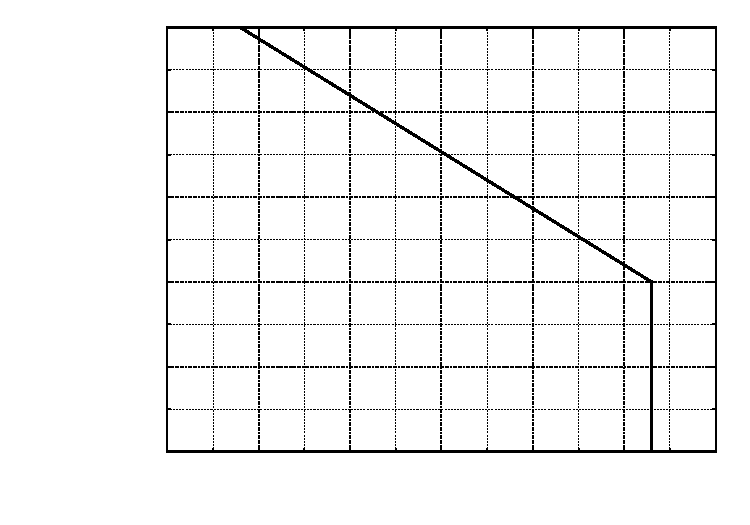
\includegraphics{../graphs/vne_chart}}%
    \gplfronttext
  \end{picture}%
\endgroup

  \end{center}  % chart from gnuplot
  \caption{$\mathrm{V_{NE}}$ vs Altitude}
  \end{figure}
\FloatBarrier

\section{AIRSPEED INDICATOR MARKINGS}

\begin{tabularx}{\textwidth}{|c|c|c|X|}
\hline 
MARKING&
ANALOG ASI&
EFIS&
SIGNIFICANCE\tabularnewline
&(KIAS)&(KIAS)&\tabularnewline

\hline
\hline 
White Arc&
48---87&
\textcolor{red}{48---87}&
Full Flap Operating Range. Lower limit is maximum weight stall speed
in landing configuration. Upper limit is maximum speed permissible
with flaps fully extended. \tabularnewline
\hline 
Green Arc&
50---168&
\textcolor{red}{50}---170&
Normal Operating Range. Lower limit is maximum weight stall speed
with flaps retracted. Upper limit is the maximum structural cruising
speed.\tabularnewline
\hline 
Yellow Arc&
168---200&
170---203&
Operations must be conducted with caution, and only in smooth air. \tabularnewline
\hline 
Red Line&
200&
203&
Maximum speed for all operations.\tabularnewline
\hline
\end{tabularx} 

\begin{Note}[NOTES]
\begin{enumerate}
\item The analog airspeed indicator markings are based on position
error estimates provided by Van's Aircraft. These markings do not account for the analog ASI instrument error (see Figure \ref{fg-asi-error}).

\item \textcolor{red}{The EFIS airspeed tape markings are to be revised
to incorporate actual position errors once these have been determined.}
\end{enumerate}
\end{Note}

\section{POWER PLANT LIMITATIONS}
The following limitations are for the Lycoming IO-360-A1B6
% No prop related RPM limits for this engine/prop combination.
\begin{longtable}[c]{@{}p{1.5in}p{4.25in}}
%\multicolumn{2}{@{}l}{Maximum Power\dotfill 200 hp}\\
\multicolumn{2}{@{}l}{Maximum Engine Speed\dotfill 2700 rpm}\\
Oil Temperature&Maximum\dotfill 245\textdegree F\\
&Desired\dotfill 180\textdegree F\\
&Minimum for continuous operation\dotfill 140\textdegree F\\
\\
\multicolumn{2}{@{}l}{Cylinder Head Temperature (CHT)}\\
&Maximum\dotfill 500\textdegree F\\
&75\% power cruise (Recommend max.)\dotfill 435\textdegree F\\
&Economy cruise  (Recommended maximum)\dotfill 400\textdegree F\\
&Recommended minimum for max. engine life\dotfill 150\textdegree F\\
\\
Oil pressure&Maximum (start, warm-up, taxi and takeoff)\dotfill115 psi\\
&Maximum (normal operations)\dotfill 95 psi\\
&Minimum (normal operations)\dotfill 55 psi\\
&Minimum (idle)\dotfill 25 psi\\
\\
Oil sump capacity&Maximum\dotfill8 US Qts\\
&Minimum safe quantity\dotfill 2 US Qts\\
\\
Fuel pressure&Maximum (at injector inlet)\dotfill 45 psi\\
&Minimum\dotfill 14 psi\\
\\
Fuel grade&Minimum Octane\dotfill 100/100LL Blue\\
\\
Propeller Diameter&Minimum\dotfill \textcolor{red}{72} inches\\
\end{longtable}


\section{ENGINE INSTRUMENT MARKINGS}
\begin{longtable}[c]{p{1.5in}p{4.25in}}
Tachometer&Green Arc --- Normal operating range. \dotfill 500 to 2700 rpm\\
&Red Line --- Maximum RPM\dotfill 2700 rpm\\
\end{longtable}

\section{EIS 4000 WARNING THRESHOLDS}
\begin{longtable}[c]{p{1.5in}p{4.25in}}
Oil Temperature&High Warning\dotfill 225\textdegree F\\
%&Low Warning \dotfill 140\textdegree F\\
\\
Oil Pressure&High Warning\dotfill 95 psi\\
% &Low Warning if rpm above \textcolor{red}{1500} rpm\dotfill 55 psi\\
% &Low Warning if rpm below \textcolor{red}{1500} rpm\dotfill 25 psi\\ 
&Low Warning\dotfill 25 psi\\ 
\\
Fuel Pressure&High Warning\dotfill 45 psi\\
&Low Warning\dotfill 14 psi\\
\\
CHT&High Warning\dotfill 450\textdegree F\\
%&Low Warning\dotfill 150\textdegree F\\
\\
RPM&High Warning\dotfill 2710 rpm\\
\\
Voltage&High Warning\dotfill 15 v\\
&Low Warning\dotfill 12 v\\
\\
Fuel Quantity&Low Level Warning\dotfill10 USG\\
\end{longtable}

\section{STARTER CRANKING LIMITATIONS}
The following limitations are for the SkyTec 149-12LS starter.
Starter cranking is limited to six 10 second cranking cycles with 20 second cool down between cranking attempts, then 30 minutes cooling.

\section{WEIGHT LIMITATIONS}
% if MTOW > 1800 lb, use this table (has line about MLW for non-paved strips)
\ifthenelse{\theMTOW > 1800}{
  \begin{longtable}[c]{p{1.5in}p{4.25in}}
    \multicolumn{2}{l}{Maximum Takeoff Weight\dotfill \theMTOW \space lb (\theMTOWkg .\theMTOWkgdecimal \space kg)}\\
    \multicolumn{2}{l}{Maximum Landing Weight\dotfill \theMTOW \space lb (\theMTOWkg .\theMTOWkgdecimal \space kg)}\\
    \multicolumn{2}{l}{Maximum weight for operations from non-paved runways\dotfill 1800 lb (816.5 kg)}\\
    \\
    \multicolumn{2}{l}{Aerobatic Gross weight (full 6g envelope available)\dotfill 1550 lb (703.1 kg)}\\
    \multicolumn{2}{l}{Restricted Aerobatic Gross weight (5g envelope available)\dotfill 1800 lb (816.5 kg)}\\
    \\
    \multicolumn{2}{l}{Maximum passenger weight\dotfill 300 lb (136 kg)}\\
    &\hfill (Subject to Weight \& Balance)\\
    \\
    \multicolumn{2}{l}{Maximum weight in forward baggage compartment\dotfill 50 lb (22.7 kg)}\\
    &\hfill (Subject to Weight \& Balance)\\
    \\
    \multicolumn{2}{l}{Maximum weight in rear baggage compartment\dotfill 75 lb (34 kg)}\\
    &\hfill (Subject to Weight \& Balance)\\
    \end{longtable}
  }
%if MTLOW <= 1800 lb, use the following table)
  {
    \begin{longtable}[c]{p{1.5in}p{4.25in}}
    \multicolumn{2}{l}{Maximum Takeoff Weight\dotfill \theMTOW \space lb (\theMTOWkg .\theMTOWkgdecimal \space kg)}\\
    \multicolumn{2}{l}{Maximum Landing Weight\dotfill \theMTOW \space lb (\theMTOWkg .\theMTOWkgdecimal \space kg)}\\
    \\
    \multicolumn{2}{l}{Aerobatic Gross weight (full 6g envelope available)\dotfill 1550 lb (703.1 kg)}\\
    \multicolumn{2}{l}{Restricted Aerobatic Gross weight (5g envelope available)\dotfill 1800 lb (816.5 kg)}\\
    \\
    \multicolumn{2}{l}{Maximum passenger weight\dotfill 300 lb (136 kg)}\\
    &\hfill (Subject to Weight \& Balance)\\
    \\
    \multicolumn{2}{l}{Maximum weight in forward baggage compartment\dotfill 50 lb (22.7 kg)}\\
    &\hfill (Subject to Weight \& Balance)\\
    \\
    \multicolumn{2}{l}{Maximum weight in rear baggage compartment\dotfill 75 lb (34 kg)}\\
    &\hfill (Subject to Weight \& Balance)\\
    \end{longtable}
  }

% only print the CAUTION if MTOW > 1800 lb
\ifthenelse{\theMTOW > 1800}
  {\begin{Note}[CAUTION]
  The maximum weight recommended by Van's Aircraft is 1800 lb  (816.5 kg).  Operations at higher weights must be conducted with caution.
  \end{Note}
   }
   {}


\begin{Note}[WARNING]
  The maximum weight recommended by Van's Aircraft for aerobatics is 1550 lb (703.1 kg).  Aerobatic operations at higher weights must respect reduced load factor limits.
  \end{Note}

\begin{Note}
  \textcolor{red}{The maximum passenger weight that is possible with the currently cleared aft CG of 85.3\char`\"{} aft of datum (aerobatic aft CG limit) is 250 lb  (113.4 kg).}
  \end{Note}



\section{CENTRE OF GRAVITY LIMITS}
\begin{longtable}[c]{p{1.5in}p{4.25in}}
\multicolumn{2}{l}{Forward limit\dotfill 15\% MAC = 78.7\char`\"{} aft of datum}\\
\multicolumn{2}{l}{Aft limit\dotfill 29\% MAC = 86.82\char`\"{} aft of datum}\\
\multicolumn{2}{l}{Aft limit for aerobatic flight\dotfill 26.5\% MAC = 85.3\char`\"{} aft of datum}\\
 & \\
\end{longtable}


\begin{Note}[NOTES]
\begin{enumerate*}
%\item The datum is 70\char`\"{} forward of the leading edge of the wing.\\
\item The datum is 70\char`\"{} forward of the leading edge of the wing.
\item  \textcolor{red}{The aft CG limit is currently restricted to  85.3\char`\"{} aft of datum (aerobatic aft CG limit) pending flight test validation of further aft CGs.}
\end{enumerate*}
\end{Note}

\begin{figure}[h!]
%\includegraphics*[viewport = 0 25 385 265]{../Diagrams/CG_envelope2.ps} % original chart from Grace
  \begin{center}
  \ifthenelse{\theMTOW > 1800}{% GNUPLOT: LaTeX picture with Postscript
\begingroup
  \makeatletter
  \providecommand\color[2][]{%
    \GenericError{(gnuplot) \space\space\space\@spaces}{%
      Package color not loaded in conjunction with
      terminal option `colourtext'%
    }{See the gnuplot documentation for explanation.%
    }{Either use 'blacktext' in gnuplot or load the package
      color.sty in LaTeX.}%
    \renewcommand\color[2][]{}%
  }%
  \providecommand\includegraphics[2][]{%
    \GenericError{(gnuplot) \space\space\space\@spaces}{%
      Package graphicx or graphics not loaded%
    }{See the gnuplot documentation for explanation.%
    }{The gnuplot epslatex terminal needs graphicx.sty or graphics.sty.}%
    \renewcommand\includegraphics[2][]{}%
  }%
  \providecommand\rotatebox[2]{#2}%
  \@ifundefined{ifGPcolor}{%
    \newif\ifGPcolor
    \GPcolorfalse
  }{}%
  \@ifundefined{ifGPblacktext}{%
    \newif\ifGPblacktext
    \GPblacktexttrue
  }{}%
  % define a \g@addto@macro without @ in the name:
  \let\gplgaddtomacro\g@addto@macro
  % define empty templates for all commands taking text:
  \gdef\gplbacktext{}%
  \gdef\gplfronttext{}%
  \makeatother
  \ifGPblacktext
    % no textcolor at all
    \def\colorrgb#1{}%
    \def\colorgray#1{}%
  \else
    % gray or color?
    \ifGPcolor
      \def\colorrgb#1{\color[rgb]{#1}}%
      \def\colorgray#1{\color[gray]{#1}}%
      \expandafter\def\csname LTw\endcsname{\color{white}}%
      \expandafter\def\csname LTb\endcsname{\color{black}}%
      \expandafter\def\csname LTa\endcsname{\color{black}}%
      \expandafter\def\csname LT0\endcsname{\color[rgb]{1,0,0}}%
      \expandafter\def\csname LT1\endcsname{\color[rgb]{0,1,0}}%
      \expandafter\def\csname LT2\endcsname{\color[rgb]{0,0,1}}%
      \expandafter\def\csname LT3\endcsname{\color[rgb]{1,0,1}}%
      \expandafter\def\csname LT4\endcsname{\color[rgb]{0,1,1}}%
      \expandafter\def\csname LT5\endcsname{\color[rgb]{1,1,0}}%
      \expandafter\def\csname LT6\endcsname{\color[rgb]{0,0,0}}%
      \expandafter\def\csname LT7\endcsname{\color[rgb]{1,0.3,0}}%
      \expandafter\def\csname LT8\endcsname{\color[rgb]{0.5,0.5,0.5}}%
    \else
      % gray
      \def\colorrgb#1{\color{black}}%
      \def\colorgray#1{\color[gray]{#1}}%
      \expandafter\def\csname LTw\endcsname{\color{white}}%
      \expandafter\def\csname LTb\endcsname{\color{black}}%
      \expandafter\def\csname LTa\endcsname{\color{black}}%
      \expandafter\def\csname LT0\endcsname{\color{black}}%
      \expandafter\def\csname LT1\endcsname{\color{black}}%
      \expandafter\def\csname LT2\endcsname{\color{black}}%
      \expandafter\def\csname LT3\endcsname{\color{black}}%
      \expandafter\def\csname LT4\endcsname{\color{black}}%
      \expandafter\def\csname LT5\endcsname{\color{black}}%
      \expandafter\def\csname LT6\endcsname{\color{black}}%
      \expandafter\def\csname LT7\endcsname{\color{black}}%
      \expandafter\def\csname LT8\endcsname{\color{black}}%
    \fi
  \fi
  \setlength{\unitlength}{0.0500bp}%
  \begin{picture}(7200.00,6300.00)%
    \gplgaddtomacro\gplbacktext{%
      \csname LTb\endcsname%
      \put(1210,704){\makebox(0,0)[r]{\strut{} 1100}}%
      \put(1210,1296){\makebox(0,0)[r]{\strut{} 1200}}%
      \put(1210,1889){\makebox(0,0)[r]{\strut{} 1300}}%
      \put(1210,2481){\makebox(0,0)[r]{\strut{} 1400}}%
      \put(1210,3073){\makebox(0,0)[r]{\strut{} 1500}}%
      \put(1210,3666){\makebox(0,0)[r]{\strut{} 1600}}%
      \put(1210,4258){\makebox(0,0)[r]{\strut{} 1700}}%
      \put(1210,4850){\makebox(0,0)[r]{\strut{} 1800}}%
      \put(1210,5443){\makebox(0,0)[r]{\strut{} 1900}}%
      \put(1210,6035){\makebox(0,0)[r]{\strut{} 2000}}%
      \put(1342,484){\makebox(0,0){\strut{} 78}}%
      \put(1895,484){\makebox(0,0){\strut{} 79}}%
      \put(2447,484){\makebox(0,0){\strut{} 80}}%
      \put(3000,484){\makebox(0,0){\strut{} 81}}%
      \put(3553,484){\makebox(0,0){\strut{} 82}}%
      \put(4106,484){\makebox(0,0){\strut{} 83}}%
      \put(4658,484){\makebox(0,0){\strut{} 84}}%
      \put(5211,484){\makebox(0,0){\strut{} 85}}%
      \put(5764,484){\makebox(0,0){\strut{} 86}}%
      \put(6316,484){\makebox(0,0){\strut{} 87}}%
      \put(6869,484){\makebox(0,0){\strut{} 88}}%
      \put(308,3369){\rotatebox{-270}{\makebox(0,0){\strut{}Weight (lb)}}}%
      \put(4105,154){\makebox(0,0){\strut{}CG (inches aft of datum)}}%
    }%
    \gplgaddtomacro\gplfronttext{%
      \put(3973,5147){\makebox(0,0){\strut{}Normal Weight/CG Envelope}}%
      \put(3553,4258){\makebox(0,0){\strut{}Restricted Aerobatic}}%
      \put(3553,3962){\makebox(0,0){\strut{}Weight/CG Envelope}}%
      \put(3553,2777){\makebox(0,0){\strut{}Aerobatic Weight/CG Envelope}}%
    }%
    \gplbacktext
    \put(0,0){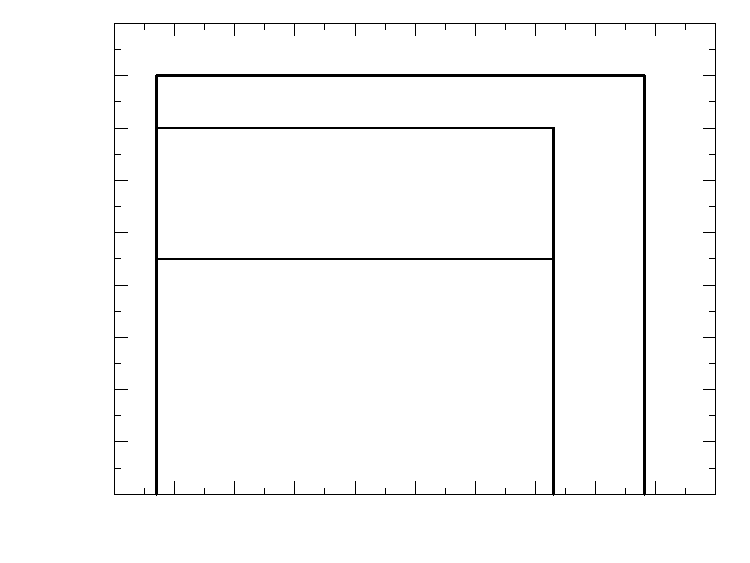
\includegraphics{../graphs/cg_chart1900}}%
    \gplfronttext
  \end{picture}%
\endgroup
}{% GNUPLOT: LaTeX picture with Postscript
\begingroup
  \makeatletter
  \providecommand\color[2][]{%
    \GenericError{(gnuplot) \space\space\space\@spaces}{%
      Package color not loaded in conjunction with
      terminal option `colourtext'%
    }{See the gnuplot documentation for explanation.%
    }{Either use 'blacktext' in gnuplot or load the package
      color.sty in LaTeX.}%
    \renewcommand\color[2][]{}%
  }%
  \providecommand\includegraphics[2][]{%
    \GenericError{(gnuplot) \space\space\space\@spaces}{%
      Package graphicx or graphics not loaded%
    }{See the gnuplot documentation for explanation.%
    }{The gnuplot epslatex terminal needs graphicx.sty or graphics.sty.}%
    \renewcommand\includegraphics[2][]{}%
  }%
  \providecommand\rotatebox[2]{#2}%
  \@ifundefined{ifGPcolor}{%
    \newif\ifGPcolor
    \GPcolorfalse
  }{}%
  \@ifundefined{ifGPblacktext}{%
    \newif\ifGPblacktext
    \GPblacktexttrue
  }{}%
  % define a \g@addto@macro without @ in the name:
  \let\gplgaddtomacro\g@addto@macro
  % define empty templates for all commands taking text:
  \gdef\gplbacktext{}%
  \gdef\gplfronttext{}%
  \makeatother
  \ifGPblacktext
    % no textcolor at all
    \def\colorrgb#1{}%
    \def\colorgray#1{}%
  \else
    % gray or color?
    \ifGPcolor
      \def\colorrgb#1{\color[rgb]{#1}}%
      \def\colorgray#1{\color[gray]{#1}}%
      \expandafter\def\csname LTw\endcsname{\color{white}}%
      \expandafter\def\csname LTb\endcsname{\color{black}}%
      \expandafter\def\csname LTa\endcsname{\color{black}}%
      \expandafter\def\csname LT0\endcsname{\color[rgb]{1,0,0}}%
      \expandafter\def\csname LT1\endcsname{\color[rgb]{0,1,0}}%
      \expandafter\def\csname LT2\endcsname{\color[rgb]{0,0,1}}%
      \expandafter\def\csname LT3\endcsname{\color[rgb]{1,0,1}}%
      \expandafter\def\csname LT4\endcsname{\color[rgb]{0,1,1}}%
      \expandafter\def\csname LT5\endcsname{\color[rgb]{1,1,0}}%
      \expandafter\def\csname LT6\endcsname{\color[rgb]{0,0,0}}%
      \expandafter\def\csname LT7\endcsname{\color[rgb]{1,0.3,0}}%
      \expandafter\def\csname LT8\endcsname{\color[rgb]{0.5,0.5,0.5}}%
    \else
      % gray
      \def\colorrgb#1{\color{black}}%
      \def\colorgray#1{\color[gray]{#1}}%
      \expandafter\def\csname LTw\endcsname{\color{white}}%
      \expandafter\def\csname LTb\endcsname{\color{black}}%
      \expandafter\def\csname LTa\endcsname{\color{black}}%
      \expandafter\def\csname LT0\endcsname{\color{black}}%
      \expandafter\def\csname LT1\endcsname{\color{black}}%
      \expandafter\def\csname LT2\endcsname{\color{black}}%
      \expandafter\def\csname LT3\endcsname{\color{black}}%
      \expandafter\def\csname LT4\endcsname{\color{black}}%
      \expandafter\def\csname LT5\endcsname{\color{black}}%
      \expandafter\def\csname LT6\endcsname{\color{black}}%
      \expandafter\def\csname LT7\endcsname{\color{black}}%
      \expandafter\def\csname LT8\endcsname{\color{black}}%
    \fi
  \fi
  \setlength{\unitlength}{0.0500bp}%
  \begin{picture}(7200.00,6300.00)%
    \gplgaddtomacro\gplbacktext{%
      \csname LTb\endcsname%
      \put(1210,704){\makebox(0,0)[r]{\strut{} 1100}}%
      \put(1210,1296){\makebox(0,0)[r]{\strut{} 1200}}%
      \put(1210,1889){\makebox(0,0)[r]{\strut{} 1300}}%
      \put(1210,2481){\makebox(0,0)[r]{\strut{} 1400}}%
      \put(1210,3073){\makebox(0,0)[r]{\strut{} 1500}}%
      \put(1210,3666){\makebox(0,0)[r]{\strut{} 1600}}%
      \put(1210,4258){\makebox(0,0)[r]{\strut{} 1700}}%
      \put(1210,4850){\makebox(0,0)[r]{\strut{} 1800}}%
      \put(1210,5443){\makebox(0,0)[r]{\strut{} 1900}}%
      \put(1210,6035){\makebox(0,0)[r]{\strut{} 2000}}%
      \put(1342,484){\makebox(0,0){\strut{} 78}}%
      \put(1895,484){\makebox(0,0){\strut{} 79}}%
      \put(2447,484){\makebox(0,0){\strut{} 80}}%
      \put(3000,484){\makebox(0,0){\strut{} 81}}%
      \put(3553,484){\makebox(0,0){\strut{} 82}}%
      \put(4106,484){\makebox(0,0){\strut{} 83}}%
      \put(4658,484){\makebox(0,0){\strut{} 84}}%
      \put(5211,484){\makebox(0,0){\strut{} 85}}%
      \put(5764,484){\makebox(0,0){\strut{} 86}}%
      \put(6316,484){\makebox(0,0){\strut{} 87}}%
      \put(6869,484){\makebox(0,0){\strut{} 88}}%
      \put(308,3369){\rotatebox{-270}{\makebox(0,0){\strut{}Weight (lb)}}}%
      \put(4105,154){\makebox(0,0){\strut{}CG (inches aft of datum)}}%
    }%
    \gplgaddtomacro\gplfronttext{%
      \put(5819,2777){\rotatebox{90}{\makebox(0,0){\strut{}Normal Weight/CG Envelope}}}%
      \put(3553,4258){\makebox(0,0){\strut{}Restricted Aerobatic}}%
      \put(3553,3962){\makebox(0,0){\strut{}Weight/CG Envelope}}%
      \put(3553,2777){\makebox(0,0){\strut{}Aerobatic Weight/CG Envelope}}%
    }%
    \gplbacktext
    \put(0,0){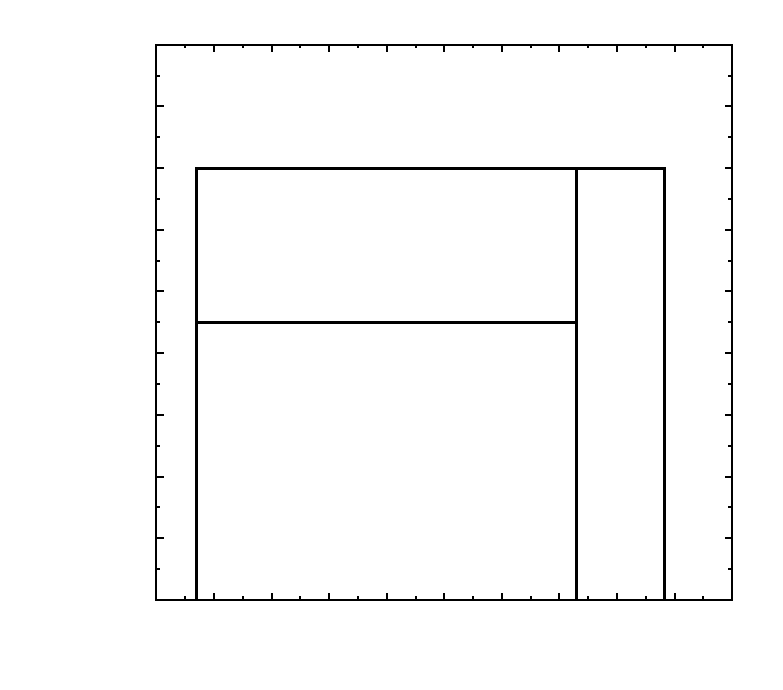
\includegraphics{../graphs/cg_chart1800}}%
    \gplfronttext
  \end{picture}%
\endgroup
}
  \end{center}  % chart from gnuplot
  \caption{Centre of Gravity Limits}
  \end{figure}
\FloatBarrier
%\pagebreak[4]
\section{MANOEUVRE LIMITS}
The following list of manoeuvres is approved when operating within the Restricted Aerobatic Weight/CG Envelope.

\begin{itemize*}
\item Upright spins, 
\item Loops, 
\item Cuban Eights, 
\item Immelmann turns, 
\item Aileron Rolls, and
\item Barrel rolls.
\end{itemize*}




% The following additional manoeuvres are approved when operating within the Aerobatic Weight/CG Envelope.

%\begin{itemize*}
%\item Hammerhead stalls, 
%\item Snap Rolls (maximum allowable entry speed
%is 95 KIAS), \item Vertical rolls, and \item Split-S (maximum allowable entry
%speed is 95 KIAS).
%\end{itemize*}
%

% \addpenalty used to suggest this is a good place to possibly break a page.
%\addpenalty{-750}
\section{LOAD FACTOR LIMITS}
\newlength{\loadcolonewidth}
\setlength{\loadcolonewidth}{0.25in}

\begin{tabular}[c]{p{.25in}p{5.5in}}
  \multicolumn{2}{l}{Load Factor Limits}\\ 
 &Flaps Up\\
  &\hspace*{\loadcolonewidth}weight 1550 lb (703.1 kg) and below:\dotfill +6g to -3g\\
  &\hspace*{\loadcolonewidth}reducing linearly to - weight  1800 lb (816.5 kg):\dotfill +5g to -2.5g\\
%  &\hspace*{\loadcolonewidth}weight 1800 lb (816.5 kg)\dotfill +5g to -2.5g\\
  \ifthenelse{\theMTOW > 1800}{
  &\hspace*{\loadcolonewidth}weight above 1800 lb (816.5 kg):\dotfill +4.4g to -2g\-\\\\
  }
  {}
  &Flaps Down\dotfill +2g to 0g\\
  \end{tabular}


\begin{NoteCtr}
  The load factor limit varies linearly between 1800 lb  (816.5 kg) and 1550 lb (703.1 kg) weight.
  \end{NoteCtr}

\begin{NoteCtr}[Caution]
  While the airframe is stressed for negative g, the engine does not have an inverted oil system.
  \end{NoteCtr}

\begin{figure}[htb]
  \begin{center}
  \ifthenelse{\theMTOW > 1800}{% GNUPLOT: LaTeX picture with Postscript
\begingroup
  \makeatletter
  \providecommand\color[2][]{%
    \GenericError{(gnuplot) \space\space\space\@spaces}{%
      Package color not loaded in conjunction with
      terminal option `colourtext'%
    }{See the gnuplot documentation for explanation.%
    }{Either use 'blacktext' in gnuplot or load the package
      color.sty in LaTeX.}%
    \renewcommand\color[2][]{}%
  }%
  \providecommand\includegraphics[2][]{%
    \GenericError{(gnuplot) \space\space\space\@spaces}{%
      Package graphicx or graphics not loaded%
    }{See the gnuplot documentation for explanation.%
    }{The gnuplot epslatex terminal needs graphicx.sty or graphics.sty.}%
    \renewcommand\includegraphics[2][]{}%
  }%
  \providecommand\rotatebox[2]{#2}%
  \@ifundefined{ifGPcolor}{%
    \newif\ifGPcolor
    \GPcolorfalse
  }{}%
  \@ifundefined{ifGPblacktext}{%
    \newif\ifGPblacktext
    \GPblacktexttrue
  }{}%
  % define a \g@addto@macro without @ in the name:
  \let\gplgaddtomacro\g@addto@macro
  % define empty templates for all commands taking text:
  \gdef\gplbacktext{}%
  \gdef\gplfronttext{}%
  \makeatother
  \ifGPblacktext
    % no textcolor at all
    \def\colorrgb#1{}%
    \def\colorgray#1{}%
  \else
    % gray or color?
    \ifGPcolor
      \def\colorrgb#1{\color[rgb]{#1}}%
      \def\colorgray#1{\color[gray]{#1}}%
      \expandafter\def\csname LTw\endcsname{\color{white}}%
      \expandafter\def\csname LTb\endcsname{\color{black}}%
      \expandafter\def\csname LTa\endcsname{\color{black}}%
      \expandafter\def\csname LT0\endcsname{\color[rgb]{1,0,0}}%
      \expandafter\def\csname LT1\endcsname{\color[rgb]{0,1,0}}%
      \expandafter\def\csname LT2\endcsname{\color[rgb]{0,0,1}}%
      \expandafter\def\csname LT3\endcsname{\color[rgb]{1,0,1}}%
      \expandafter\def\csname LT4\endcsname{\color[rgb]{0,1,1}}%
      \expandafter\def\csname LT5\endcsname{\color[rgb]{1,1,0}}%
      \expandafter\def\csname LT6\endcsname{\color[rgb]{0,0,0}}%
      \expandafter\def\csname LT7\endcsname{\color[rgb]{1,0.3,0}}%
      \expandafter\def\csname LT8\endcsname{\color[rgb]{0.5,0.5,0.5}}%
    \else
      % gray
      \def\colorrgb#1{\color{black}}%
      \def\colorgray#1{\color[gray]{#1}}%
      \expandafter\def\csname LTw\endcsname{\color{white}}%
      \expandafter\def\csname LTb\endcsname{\color{black}}%
      \expandafter\def\csname LTa\endcsname{\color{black}}%
      \expandafter\def\csname LT0\endcsname{\color{black}}%
      \expandafter\def\csname LT1\endcsname{\color{black}}%
      \expandafter\def\csname LT2\endcsname{\color{black}}%
      \expandafter\def\csname LT3\endcsname{\color{black}}%
      \expandafter\def\csname LT4\endcsname{\color{black}}%
      \expandafter\def\csname LT5\endcsname{\color{black}}%
      \expandafter\def\csname LT6\endcsname{\color{black}}%
      \expandafter\def\csname LT7\endcsname{\color{black}}%
      \expandafter\def\csname LT8\endcsname{\color{black}}%
    \fi
  \fi
  \setlength{\unitlength}{0.0500bp}%
  \begin{picture}(7200.00,5040.00)%
    \gplgaddtomacro\gplbacktext{%
      \csname LTb\endcsname%
      \put(814,704){\makebox(0,0)[r]{\strut{}-4}}%
      \csname LTb\endcsname%
      \put(814,1444){\makebox(0,0)[r]{\strut{}-2}}%
      \csname LTb\endcsname%
      \put(814,2184){\makebox(0,0)[r]{\strut{} 0}}%
      \csname LTb\endcsname%
      \put(814,2925){\makebox(0,0)[r]{\strut{} 2}}%
      \csname LTb\endcsname%
      \put(814,3665){\makebox(0,0)[r]{\strut{} 4}}%
      \csname LTb\endcsname%
      \put(814,4405){\makebox(0,0)[r]{\strut{} 6}}%
      \csname LTb\endcsname%
      \put(946,484){\makebox(0,0){\strut{} 1100}}%
      \csname LTb\endcsname%
      \put(1604,484){\makebox(0,0){\strut{} 1200}}%
      \csname LTb\endcsname%
      \put(2262,484){\makebox(0,0){\strut{} 1300}}%
      \csname LTb\endcsname%
      \put(2920,484){\makebox(0,0){\strut{} 1400}}%
      \csname LTb\endcsname%
      \put(3578,484){\makebox(0,0){\strut{} 1500}}%
      \csname LTb\endcsname%
      \put(4237,484){\makebox(0,0){\strut{} 1600}}%
      \csname LTb\endcsname%
      \put(4895,484){\makebox(0,0){\strut{} 1700}}%
      \csname LTb\endcsname%
      \put(5553,484){\makebox(0,0){\strut{} 1800}}%
      \csname LTb\endcsname%
      \put(6211,484){\makebox(0,0){\strut{} 1900}}%
      \csname LTb\endcsname%
      \put(6869,484){\makebox(0,0){\strut{} 2000}}%
      \put(308,2739){\rotatebox{-270}{\makebox(0,0){\strut{}Load Factor Limit (g)}}}%
      \put(3907,154){\makebox(0,0){\strut{}Weight (lb)}}%
    }%
    \gplgaddtomacro\gplfronttext{%
    }%
    \gplbacktext
    \put(0,0){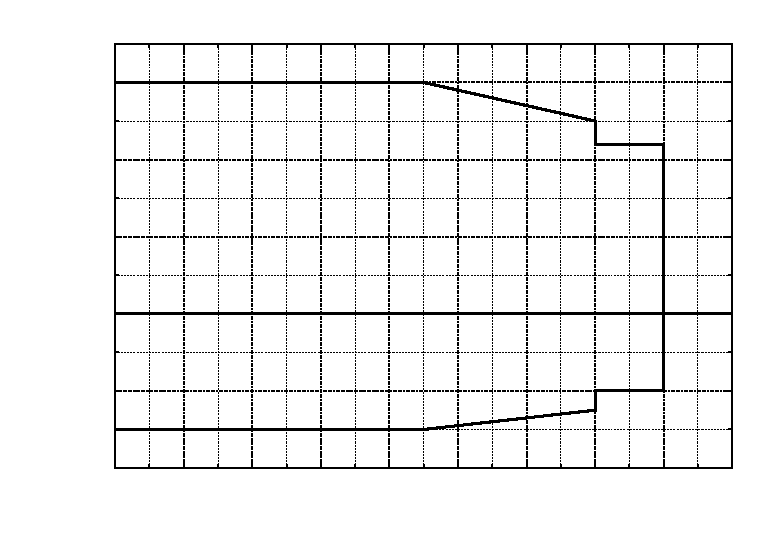
\includegraphics{../graphs/g-chart1900}}%
    \gplfronttext
  \end{picture}%
\endgroup
}{% GNUPLOT: LaTeX picture with Postscript
\begingroup
  \makeatletter
  \providecommand\color[2][]{%
    \GenericError{(gnuplot) \space\space\space\@spaces}{%
      Package color not loaded in conjunction with
      terminal option `colourtext'%
    }{See the gnuplot documentation for explanation.%
    }{Either use 'blacktext' in gnuplot or load the package
      color.sty in LaTeX.}%
    \renewcommand\color[2][]{}%
  }%
  \providecommand\includegraphics[2][]{%
    \GenericError{(gnuplot) \space\space\space\@spaces}{%
      Package graphicx or graphics not loaded%
    }{See the gnuplot documentation for explanation.%
    }{The gnuplot epslatex terminal needs graphicx.sty or graphics.sty.}%
    \renewcommand\includegraphics[2][]{}%
  }%
  \providecommand\rotatebox[2]{#2}%
  \@ifundefined{ifGPcolor}{%
    \newif\ifGPcolor
    \GPcolorfalse
  }{}%
  \@ifundefined{ifGPblacktext}{%
    \newif\ifGPblacktext
    \GPblacktexttrue
  }{}%
  % define a \g@addto@macro without @ in the name:
  \let\gplgaddtomacro\g@addto@macro
  % define empty templates for all commands taking text:
  \gdef\gplbacktext{}%
  \gdef\gplfronttext{}%
  \makeatother
  \ifGPblacktext
    % no textcolor at all
    \def\colorrgb#1{}%
    \def\colorgray#1{}%
  \else
    % gray or color?
    \ifGPcolor
      \def\colorrgb#1{\color[rgb]{#1}}%
      \def\colorgray#1{\color[gray]{#1}}%
      \expandafter\def\csname LTw\endcsname{\color{white}}%
      \expandafter\def\csname LTb\endcsname{\color{black}}%
      \expandafter\def\csname LTa\endcsname{\color{black}}%
      \expandafter\def\csname LT0\endcsname{\color[rgb]{1,0,0}}%
      \expandafter\def\csname LT1\endcsname{\color[rgb]{0,1,0}}%
      \expandafter\def\csname LT2\endcsname{\color[rgb]{0,0,1}}%
      \expandafter\def\csname LT3\endcsname{\color[rgb]{1,0,1}}%
      \expandafter\def\csname LT4\endcsname{\color[rgb]{0,1,1}}%
      \expandafter\def\csname LT5\endcsname{\color[rgb]{1,1,0}}%
      \expandafter\def\csname LT6\endcsname{\color[rgb]{0,0,0}}%
      \expandafter\def\csname LT7\endcsname{\color[rgb]{1,0.3,0}}%
      \expandafter\def\csname LT8\endcsname{\color[rgb]{0.5,0.5,0.5}}%
    \else
      % gray
      \def\colorrgb#1{\color{black}}%
      \def\colorgray#1{\color[gray]{#1}}%
      \expandafter\def\csname LTw\endcsname{\color{white}}%
      \expandafter\def\csname LTb\endcsname{\color{black}}%
      \expandafter\def\csname LTa\endcsname{\color{black}}%
      \expandafter\def\csname LT0\endcsname{\color{black}}%
      \expandafter\def\csname LT1\endcsname{\color{black}}%
      \expandafter\def\csname LT2\endcsname{\color{black}}%
      \expandafter\def\csname LT3\endcsname{\color{black}}%
      \expandafter\def\csname LT4\endcsname{\color{black}}%
      \expandafter\def\csname LT5\endcsname{\color{black}}%
      \expandafter\def\csname LT6\endcsname{\color{black}}%
      \expandafter\def\csname LT7\endcsname{\color{black}}%
      \expandafter\def\csname LT8\endcsname{\color{black}}%
    \fi
  \fi
  \setlength{\unitlength}{0.0500bp}%
  \begin{picture}(7200.00,5040.00)%
    \gplgaddtomacro\gplbacktext{%
      \csname LTb\endcsname%
      \put(814,704){\makebox(0,0)[r]{\strut{}-4}}%
      \csname LTb\endcsname%
      \put(814,1444){\makebox(0,0)[r]{\strut{}-2}}%
      \csname LTb\endcsname%
      \put(814,2184){\makebox(0,0)[r]{\strut{} 0}}%
      \csname LTb\endcsname%
      \put(814,2925){\makebox(0,0)[r]{\strut{} 2}}%
      \csname LTb\endcsname%
      \put(814,3665){\makebox(0,0)[r]{\strut{} 4}}%
      \csname LTb\endcsname%
      \put(814,4405){\makebox(0,0)[r]{\strut{} 6}}%
      \csname LTb\endcsname%
      \put(946,484){\makebox(0,0){\strut{} 1100}}%
      \csname LTb\endcsname%
      \put(1604,484){\makebox(0,0){\strut{} 1200}}%
      \csname LTb\endcsname%
      \put(2262,484){\makebox(0,0){\strut{} 1300}}%
      \csname LTb\endcsname%
      \put(2920,484){\makebox(0,0){\strut{} 1400}}%
      \csname LTb\endcsname%
      \put(3578,484){\makebox(0,0){\strut{} 1500}}%
      \csname LTb\endcsname%
      \put(4237,484){\makebox(0,0){\strut{} 1600}}%
      \csname LTb\endcsname%
      \put(4895,484){\makebox(0,0){\strut{} 1700}}%
      \csname LTb\endcsname%
      \put(5553,484){\makebox(0,0){\strut{} 1800}}%
      \csname LTb\endcsname%
      \put(6211,484){\makebox(0,0){\strut{} 1900}}%
      \csname LTb\endcsname%
      \put(6869,484){\makebox(0,0){\strut{} 2000}}%
      \put(308,2739){\rotatebox{-270}{\makebox(0,0){\strut{}Load Factor Limit (g)}}}%
      \put(3907,154){\makebox(0,0){\strut{}Weight (lb)}}%
    }%
    \gplgaddtomacro\gplfronttext{%
    }%
    \gplbacktext
    \put(0,0){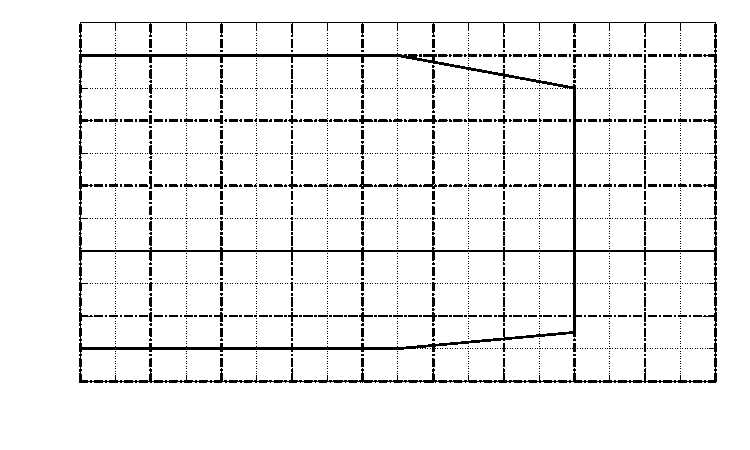
\includegraphics{../graphs/g-chart1800}}%
    \gplfronttext
  \end{picture}%
\endgroup
}
  \end{center}  % chart from gnuplot
  \caption{Load Factor Limit vs Weight}
  \end{figure}
  
\begin{Note}[NOTES]
  \begin{enumerate}
    \item The load factor limits for weights above 1550 lb (703.1 kg) are not published by
Van's Aircraft, but are established based on conservative engineering
analysis of wing bending moment vs load factor. 
    \item The load factor limits for flaps down are based on FAR
23 structural design criteria, which the RV-8 is designed to.  
    \end{enumerate}
  \end{Note}

\section{KINDS OF OPERATION LIMITS}

The airplane is approved for:
\begin{itemize*}
\item Day VFR,
\item Night VFR (\textcolor{red}{subject to flight test validation of night lighting}), 
\item Day IFR, and 
\item Night IFR (\textcolor{red}{subject to flight test validation of night lighting}).
\end{itemize*}
Flight in known or forecast icing conditions is prohibited.


\section{FUEL LIMITATIONS}
\begin{quote}
Total capacity\dotfill 163.5 l (43.2 USG)\\
Usable fuel\dotfill 43 USG\\
Unusable fuel\dotfill 0.2 USG\\
Approved fuels\dotfill 100/130 - Green\\
%\raggedleft 100 - Green\\
%100LL - Blue\\
\hspace*{\fill}100 - Green\\
\hspace*{\fill}100LL - Blue\\
\end{quote}

It is prohibited to select the left tank for takeoff or landing
unless there are at least \textcolor{red}{10 USG} of fuel remaining in the selected tank.  

%\section{ELECTRICAL LIMITATIONS}
%Aux Power -- The Aux Power receptacle is limited to 10 amps maximum.

\section{GNS 430W LIMITATIONS}
%
%  The Main software version is displayed on the GNS 430W self test page immediately after turn-on for 5 seconds.  The remaining system software versions can be verified on the AUX group sub-page 2, "SOFTWARE/DATABASE VER".


  IFR enroute and terminal navigation predicated upon the GNS 430W's GPS receiver is prohibited unless the pilot verifies the currency of the data base or verifies each selected waypoint for accuracy by reference to current approved data.
  
  Operations on RNAV STARs are prohibited unless the autopilot is engaged in TRK mode (TC AIM RAC 9.2.2 \& FAA AC 90-100A para 10(b)(9)).
  
  Instrument approach navigation predicated upon the GNS 430W's GPS receiver must be accomplished in accordance with approved instrument approach procedures that are retrieved from the GNS 430W's data base.  The GNS 430W's database must incorporate the current update cycle.
  \begin{enumerate}
    \item Instrument approaches utilizing the GPS receiver must be conducted in the Approach Mode and Receiver Autonomous Integrity Monitoring (RAIM) must be available at the Final Approach Fix.
    \item Accomplishment of ILS, LOC, LOC-BC, LDA, SDF, MLS or any other type of approach not approved for GPS overlay with the GNS 430W's GPS receiver is not authorized.
    \item Use of the GNS 430W's VOR/ILS receiver to fly approaches not approved for GPS require VOR/ILS navigation data to be displayed on the external indicator.
    \item VNAV information may be utilized for advisory information only. Use of VNAV information for instrument approach procedures does not guarantee step-down fix altitude protection, or arrival at approach minimums in normal position to land.
    \end{enumerate}
  If not previously defined, the following default settings must be made in the ``SETUP 1'' menu of the GNS 430W prior to operation (refer to GNS 430W Pilot's Guide for procedure if necessary):

  \begin{tabular}{ll}
     \textbf{dis, spd} &nm, kt (sets navigation units to ``nautical miles'' and ``knots'')\\
     \textbf{alt, vs} &ft, fpm (sets altitude units to ``feet'' and ``feet per minute'')\\
     \textbf{map datum} &WGS 84 (sets map datum to WGS-84)\\
     \textbf{posn} &deg-min (sets navigation grid units to decimal minutes)\\
     \end{tabular}

\section{AUTOPILOT LIMITATIONS}
Minimum engage height: 400 ft AGL.

%Preflight override test must be conducted if wing leveler is to be used on that flight.
Use of the autopilot in-flight is prohibited unless pre-flight override tests were conducted on both pitch and roll axis.
%\textcolor{red}{add more if required}
\clearpage
\section{PLACARDS}
The following information is displayed by placards:

\settowidth{\colOne}{Forward Baggage Area}
%\setlength{\colTwo}{\textwidth-\colOne-24pt}
%%\setlength{\colTwo}{4in}

\begin{tabularx}{\textwidth}{p{\colOne}X}
  \textbf{Location}&\textbf{Placard}\\
  Front Seat&THE FOLLOWING  AEROBATIC MANOEUVRES, AND COMBINATIONS THEREOF, MAY BE PERFORMED IN THIS AEROPLANE:\\
 % \textcolor{red}{(List approved manoeuvres, once they are defined - see AMA 549.101A \S5a.)}\\
&\begin{itemize*}
\item UPRIGHT SPINS, 
\item LOOPS, 
\item CUBAN EIGHTS, 
\item IMMELMANN TURNS, 
\item AILERON ROLLS, AND
\item BARREL ROLLS.
\end{itemize*}\\
  \raggedright Ahead of Throttle Quadrant&
  \begin{tabular}{ccccc}
    \multicolumn{5}{c}{MAXIMUM POWER MIXTURE}\\
    ALTITUDE&S.L.&4000&8000&12,000\\
    US GAL/HR&17&15&13&10\\
    \end{tabular}\\\\
  \raggedright Rear Seat& YOU FLY IN THIS AIRCRAFT AT YOUR OWN RISK.  THIS AIRCRAFT DOES NOT COMPLY WITH INTERNATIONALLY RECOGNIZED STANDARDS. VOUS VOLEZ \`{A} BORD DE CET A\'{E}RONEF  \`{A} VOS PROPRES RISQUES.  CET A\'{E}RONEF N�EST PAS CONFORME AUX NORMES RECONNUES  \`{A} L�\'{E}CHELLE INTERNATIONALE.\\\\
  % Rear Seat& PASSENGERS PROHIBITED \textcolor{red}{(Placard only required during Flight Test Phase)} \\\\
  Rear Seat&MAXIMUM  PASSENGER LOAD 136 KG (300  LB)\\\\
  Forward Baggage Area&MAXIMUM BAGGAGE LOAD 23 KG (50 LB)\\\\
  Aft Baggage Area&MAXIMUM BAGGAGE LOAD 34 KG (75 LB)\\\\
  % By Fuel Tank Cap&FUEL CAPACITY \textcolor{red}{159} L 100 LL OR 100/130 \textcolor{red}{(Check required wording.)}
  \end{tabularx}

\cleardoublepage

% !iTeXMac(input): POH.tex
\chapter{EMERGENCY PROCEDURES}
\vspace{\minitocspacebefore}
\minitoc
\cleardoublepage
\section{INTRODUCTION}
Section 3 provides procedures to address emergencies that may occur.   Should an emergency arise, the basic guidelines in this section should be considered and applied as necessary to correct the problem.

Some emergency procedures receive additional discussion in the Amplified Procedures section which follows the Emergency Checklists.

\section{AIRSPEEDS FOR EMERGENCY OPERATION}
(\textcolor{red}{Red text indicates provisional information, based
on the RV-8A Aircraft Performance Report published by the CAFE Foundation. This data has not yet been validated by flight test.})

\begin{quote}
Engine Failure After Takeoff\\
\newlength\emertab
\setlength\emertab{0.2in}
%\hspace{\emertab}Flaps UP\dotfill \textcolor{red}{XX} KIAS\\
\hspace*{\emertab}Flaps UP\dotfill 115 KIAS\\
\hspace*{\emertab}Flaps DOWN\dotfill 80 KIAS\\
Manoeuvring Speed\\
\hspace*{\emertab}1550 lb (703.1 kg) or greater\dotfill \textcolor{red}{120} KIAS\\
\hspace*{\emertab}1300 lb (589.7 kg)\dotfill \textcolor{red}{110} KIAS\\
Maximum Glide\\
\hspace*{\emertab}\theMTOW \space lb (\theMTOWkg .\theMTOWkgdecimal \space kg)\dotfill 115 KIAS\\
\hspace*{\emertab}1600 lb (725.7 kg)\dotfill 105 KIAS\\
\hspace*{\emertab}1300 lb (589.7 kg)\dotfill 95 KIAS\\
Precautionary Landing With Engine Power\dotfill 70 KIAS\\
Landing Without Engine Power\\
\hspace*{\emertab}Flaps UP\dotfill 115 KIAS\\
\hspace*{\emertab}Flaps DOWN\dotfill 80 KIAS
\end{quote}

\cleardoublepage
% !iTeXMac(input): POH.tex
\changepage{\checklistTextHeight}{\checklistTextWidth}{\checklistEvenSideMargin}{\checklistOddSideMargin}{}{\checklistTopMargin}{0pt}{0pt}{0pt}% original settings, with no room for header or footer

%% next three lines show a mini page diagram with margins
%\currentpage
%\setlayoutscale{0.5}
%\pagedesign

\small
%\footnotesize
%\addcontentsline{toc}{section}{\numberline { }EMERGENCY CHECKLIST}
%\addcontentsline{toc}{section}{\numberline EMERGENCY CHECKLIST}
\addcontentsline{toc}{section}{EMERGENCY CHECKLISTS}
%\mtcaddsection[EMERGENCY CHECKLIST]
\chead{\Large EMERGENCY CHECKLISTS} % puts "EMERGENCY CHECKLIST" in the header.
% \ohead{DRAFT --- \thistime \ \cdndate\today}
\ohead{Created --- \thistime \ \cdndate\today}

\begin{multicols}{2}

%\section{EMERGENCY CHECKLISTS} % leave this line commented out, 
%as it destroys the visual flow of the checklist page.
% Find a way to get "EMERGENCY CHECKLISTS" in the header instead.
\subsection*{ENGINE FAILURES}
%\renewcommand\sectionmark{\markright {EMERGENCY CHECKLISTS}}


\subsubsection*{\fcolorbox{black}{red}{ENGINE FAILURE DURING TAKEOFF RUN}}

\begin{enumerate*}
  \item Throttle \dotfill IDLE
  \item Brakes \dotfill APPLY
  \item Flaps \dotfill RETRACT
  \item \emph{If insufficient runway remains:}
  \begin{itemize*}
%    \item Mixture \dotfill IDLE CUT-OFF
    \item Fuel Selector \dotfill OFF
    \item Ignition Switches (Both) \dotfill OFF
    \item BATT/ALT \dotfill OFF
    \end{itemize*}
  \end{enumerate*}

\subsubsection*{\fcolorbox{black}{red}{ENGINE FAILURE IMMEDIATELY AFTER TAKEOFF}}

\begin{enumerate*}
\item Airspeed \raggedright \dotfill 115 KIAS (Flaps UP)\\\hfill80 KIAS (Flaps DOWN)
\item Mixture \dotfill IDLE CUT-OFF
\item Prop \dotfill MIN RPM
\item Fuel Selector \dotfill OFF
\item Ignition Switches (Both) \dotfill OFF
\item Flaps \dotfill AS REQUIRED
\item BATT/ALT \dotfill OFF
\end{enumerate*}

\subsubsection*{\fcolorbox{black}{red}{ENGINE FAILURE DURING FLIGHT}}

\begin{enumerate*}
\item Airspeed \dotfill 115 KIAS
\item Fuel Selector \dotfill SWITCH TANKS
\item Boost Pump \dotfill ON
\item Mixture \dotfill RICH
\item Alternate Air \dotfill ON
% \item Left Ignition Switch \dotfill ON, OFF, ON
% \item Right Ignition Switch \dotfill ON, OFF, ON
\item IGNITION, ELEC \dotfill ON, OFF, ON
\item IGNITION, MAG \dotfill ON, OFF, ON
\item Starter \dotfill START (if propeller is stopped)
\item Transponder\dotfill 7700
\end{enumerate*}

\subsubsection*{\fcolorbox{black}{yellow}{ROUGH RUNNING ENGINE}}

\begin{enumerate*}
\item Mixture \dotfill ADJUST
\item Throttle \dotfill ADJUST
\item Boost Pump \dotfill ON
\item Fuel Selector \dotfill CHANGE TANKS
\item Alternate Air \dotfill ON
\suspend{enumerate*}
\begin{Note}[CAUTION]
If engine quits when ignition selected OFF, select the mixture to ICO, wait 10 seconds, then select the ignition back ON.
Advance mixture slowly until engine restarts.
\end{Note}
\resume{enumerate*}
% \item Left Ignition Switch \dotfill ON, OFF, ON
% \item Right Ignition Switch \dotfill ON, OFF, ON
\item IGNITION, ELEC \dotfill ON, OFF, ON
\item IGNITION, MAG \dotfill ON, OFF, ON
\item Prepare for power off landing
\end{enumerate*}

\subsubsection*{\fcolorbox{black}{yellow}{HIGH OIL TEMPERATURE}}

\begin{enumerate*}
\item Oil Cooler Door \dotfill OPEN
\item Oil temperature and pressure \dotfill MONITOR
\end{enumerate*}

\subsubsection*{\fcolorbox{black}{yellow}{LOW FUEL PRESSURE}}

\begin{enumerate*}
\item Boost Pump \dotfill ON
\item Fuel Selector \dotfill CHANGE TANKS
\end{enumerate*}

\subsubsection*{\fcolorbox{black}{yellow}{LOW OIL PRESSURE}}

\begin{enumerate*}
\item OIL PRESS light \dotfill CHECK
\item EIS Oil Pressure Indication \dotfill CHECK
\suspend{enumerate*}
%\begin{Note}
%EIS oil pressure and OIL PRESS light use different transducers. In
%case of discrepancy, suspect false warning.
%\end{Note}
\begin{Note}
In case of discrepancy between indications, suspect false warning.
\end{Note}
\resume{enumerate*}
\item \emph{If both indications confirm low oil pressure:}
\begin{itemize*}
  \item Land ASAP
  \end{itemize*}
\end{enumerate*}

\subsubsection*{\fcolorbox{black}{yellow}{AIR-START}}

\begin{enumerate*}
  \item Throttle \dotfill 1/4 OPEN
  \item Prop \dotfill MAX RPM
  \item Fuel Pressure \dotfill CHECK
  \item \emph{If fuel pressure less than 14 psi:}
  \begin{itemize*}
    \item Boost Pump \dotfill ON
    \item Fuel Selector \dotfill CHANGE TANKS
    \end{itemize*}
  \item Ignition Switches\dotfill BOTH ON
  \item Mixture \dotfill IDLE CUT-OFF
%  \item Mixture \raggedright \dotfill ADVANCE SLOWLY\\\hfill UNTIL ENGINE STARTS
  \item Mixture \dotfill ADVANCE SLOWLY UNTIL ENGINE STARTS
  \item \emph{When engine starts:}
  \begin{itemize*}
    \item Throttle \dotfill A/R
    \item Boost Pump \dotfill OFF
    \end{itemize*}
  
  \end{enumerate*}

\subsection*{FORCED LANDINGS}
\subsubsection*{\fcolorbox{black}{red}{EMERGENCY LANDING WITHOUT POWER}}

\begin{enumerate*}
\item Airspeed \raggedright \dotfill 115 KIAS (Flaps UP)\\\hfill80 KIAS (Flaps DOWN)
\item Throttle \dotfill CLOSED
\item Mixture \dotfill IDLE CUT-OFF
\item Prop \dotfill MIN RPM
\item Fuel Selector \dotfill OFF
\item Ignition Switches (Both) \dotfill OFF
\item Radio \dotfill TRANSMIT MAYDAY
\item Flaps \dotfill A/R
\item BATT/ALT \dotfill OFF
\end{enumerate*}

\subsubsection*{\fcolorbox{black}{yellow}{EMERGENCY LANDING WITH POWER}}

\begin{enumerate*}
\item Radio \dotfill TRANSMIT MAYDAY
\item Airspeed \dotfill 85 KIAS
\item Flaps \dotfill 50\%
\item Selected Field \dotfill FLY OVER
\item Flaps \dotfill FULL
\item Airspeed \dotfill 70 KIAS
\item BATT/ALT \dotfill OFF
\item Ignition Switches (Both) \dotfill OFF (after touchdown)
\end{enumerate*}

%\clearpage

\subsubsection*{\fcolorbox{black}{red}{DITCHING}}

\begin{enumerate*}
\item Radio \dotfill TRANSMIT MAYDAY
\item Flaps \dotfill FULL
\item Airspeed \dotfill 70 KIAS
\item Power \dotfill 300 FT/MIN DESCENT
%\item Approach - High Wind \dotfill INTO WIND
%\item - Light Wind \dotfill PARALLEL TO SWELLS
\item Approach \raggedright \dotfill High Wind - INTO WIND\\\hfill Light Wind - PARALLEL TO SWELLS
\item Face \dotfill CUSHION with folded coat
\item \emph{Leaving Aircraft}

\begin{itemize*}
  \item Seat Belts \dotfill RELEASE
  \item Canopy \dotfill OPEN
  \item Aircraft \dotfill EXIT
  \item Life Jacket \dotfill INFLATE 
  \end{itemize*}
\end{enumerate*}

\subsection*{FIRES}
\subsubsection*{\fcolorbox{black}{red}{FIRE DURING START ON GROUND}}
\begin{enumerate*}
  % \item Boost Pump \dotfill OFF
  \item Mixture \dotfill IDLE CUT-OFF
  \item Fuel Selector \dotfill OFF
  \item Starter \dotfill OFF
  \item BATT/ALT \dotfill OFF
  \item Fire Extinguisher\dotfill OBTAIN
  \item Aircraft\dotfill EVACUATE
  \item Fire\dotfill EXTINGUISH
  \end{enumerate*}

\subsubsection*{\fcolorbox{black}{red}{ENGINE FIRE IN FLIGHT}}
\begin{enumerate*}
\item Mixture \dotfill IDLE CUT-OFF
\item Fuel Selector \dotfill OFF
\item Boost Pump \dotfill OFF
\item Cabin Heat and Air \dotfill OFF
\item ESS BUS FEED \dotfill EMER
\item BATT/ALT \dotfill OFF
\item Forced Landing \dotfill COMPLETE
\end{enumerate*}

\subsubsection*{\fcolorbox{black}{red}{ELECTRICAL FIRE IN FLIGHT}}

\begin{enumerate*}
\item BATT/ALT \dotfill OFF
\item STBY ALT \dotfill OFF
\item ESS BUS FEED \dotfill NORM
\item EFIS auto-shutdown \dotfill OVERRIDE (if EFIS required)
\item Avionics \dotfill OFF
\item All Other Switches (except Mag and TURN COORD)\dotfill OFF
\item Vents/ Cabin Air/ Heat \dotfill CLOSED
\item Fire Extinguisher \dotfill ACTIVATE
\item Cabin \dotfill VENTILATE
\end{enumerate*}

\begin{Note}[WARNING]
  Ventilate the cockpit ASAP after discharging the fire extinguisher.
  \end{Note}
  
\subsubsection*{\fcolorbox{black}{red}{CABIN FIRE}}

\begin{enumerate*}
\item BATT/ALT \dotfill OFF
\item STBY ALT \dotfill OFF
\item ESS BUS FEED \dotfill NORM
\item EFIS auto-shutdown \dotfill OVERRIDE (if EFIS required)
\item Vents/ Cabin Heat \dotfill CLOSED
\item Fire Extinguisher \dotfill ACTIVATE
\item Cabin \dotfill VENTILATE
\end{enumerate*}

\begin{Note}[WARNING]
  Ventilate the cockpit ASAP after discharging the fire extinguisher.
  \end{Note}
  
\subsubsection*{\fcolorbox{black}{red}{WING FIRE}}

\begin{enumerate*}
\item Nav/Strobe Light Switch \dotfill OFF
\item Landing \& Taxi Lights \dotfill OFF
\item PITOT HEAT \dotfill OFF
\end{enumerate*}

\begin{Note}
  Perform a sideslip to keep the flames away from the fuel tank and cockpit, and land as soon as possible.
  \end{Note}

\subsection*{OTHER}
\subsubsection*{\fcolorbox{black}{yellow}{STATIC SOURCE BLOCKAGE}}
\begin{enumerate*}
  \item Vents/ Cabin Air/ Heat \dotfill CLOSED
  \item Alternate Static Source Valve\dotfill  OPEN
  \item Airspeed and altitude corrections\dotfill  APPLY
  \end{enumerate*}

\columnbreak
\subsubsection*{\fcolorbox{black}{yellow}{ALTERNATOR FAILURE}}

\begin{enumerate*}
\item BATT/ALT \dotfill BATT, then BATT + ALT
\item \emph{If failure continues:}

\begin{itemize*}
\item ESS BUS FEED \dotfill EMER
\item \emph{If instrument lighting required:}

\begin{itemize*}
\item[\textbullet] Map Light \dotfill ON
\end{itemize*}
\item Radios \dotfill SELECT COM 1 (GNS 430)
\item BATT/ALT \dotfill OFF
\item STBY ALT \dotfill ON
\item EFIS BU \dotfill ON
\item Voltage \dotfill MONITOR
%\item \emph{Prior to landing, if Main Bus powered equipment is required:}
%\begin{itemize*}
%\item BATT/ALT \dotfill ON
%\end{itemize*}
\item The following Main Bus powered equipment is inoperative:

\begin{tabular}{ll}
COM 2&Landing and Taxi Lights\\
Intercom&CDI Lighting\\
Pitot Heat&Eng. Instrument Lighting\\
Flaps&Strobe Lights\\
Boost Pump&Position Lights\\
Analog Tach and MP&Low Oil Press. Light\\
Autopilot&Defrost Fan\\
\end{tabular}
\item \emph{Prior to landing, if equipment powered from Main Bus is required:}
\begin{itemize*}
\item BATT/ALT \dotfill ON
\end{itemize*}
\end{itemize*}
\end{enumerate*}

\subsubsection*{\fcolorbox{black}{yellow}{STARTER ENGAGED LIGHT ILLUMINATED}}
\begin{enumerate*}
  \item BATT/ALT \dotfill OFF
  \item Aircraft \dotfill LAND ASAP
  \end{enumerate*}

\subsubsection*{\fcolorbox{black}{red}{AUTOPILOT MALFUNCTION}}
\begin{enumerate*}
  \item Trim/Autopilot Cut-out \dotfill PRESS AND HOLD
  \item Autopilot Power Switch (Autopilot Control Head)\dotfill OFF
  \item WING LVLR Switch (Right Console)\dotfill OFF
  \item Trim/Autopilot Cut-out \dotfill RELEASE
%  \item \emph{If failure continues:}
%  \begin{itemize*}
%    \item Wing Leveler/Control Stick ``pip'' Pin \dotfill PULL
%    \end{itemize*}
  \end{enumerate*}

\subsubsection*{\fcolorbox{black}{red}{RUNAWAY TRIM}}
\begin{enumerate*}
  \item Trim/Autopilot Cut-out \dotfill PRESS AND HOLD
  \item TRIM Switch \dotfill OFF
  \item Trim/Autopilot Cut-out \dotfill RELEASE
  \end{enumerate*}

\subsubsection*{\fcolorbox{black}{red}{AIRBORNE EGRESS}}

\begin{enumerate*}
\item Helmet Jacks \dotfill UNPLUG
\item Canopy Jettison Pins \dotfill REMOVE
\item Canopy \dotfill UNLATCH \& PULL AFT
\item Canopy \dotfill PUSH UP (lower head)
\item Seat Belt \dotfill RELEASE
\item Aircraft \dotfill EGRESS
\end{enumerate*}

\subsubsection*{\fcolorbox{black}{red}{CO MONITOR ALARM}}
\begin{enumerate*}
\item Power \dotfill REDUCE
\item Mixture \dotfill WELL LEAN OF PEAK
\item Cabin Heat (Both) \dotfill CLOSED
\item Fresh Air Vents (Both) \dotfill OPEN
\item CO Monitor \dotfill MONITOR READINGS
\item \emph{If red light on CO Monitor remains illuminated:}

  \begin{itemize*}
    \item Airspeed \dotfill 80 KT MAX
    \item Canopy \dotfill OPEN SLIGHTLY
    \end{itemize*}
\end{enumerate*}
\end{multicols}


%\cleardoublepage
\normalsize
\cleardoublepage
\ohead{\leftmark} % put Section name back in outer header
\chead{} % remove center header
\changepage{\checklistTextHeight*-1}{\checklistTextWidth*-1}{\checklistEvenSideMargin*-1}{\checklistOddSideMargin*-1}{}{\checklistTopMargin*-1}{0pt}{0pt}{0pt}% original settings, with no room for header or footer


%\cleardoublepage

\section{AMPLIFIED EMERGENCY PROCEDURES}

\subsection{ENGINE FAILURES}
\subsubsection{ENGINE POWER LOSS DURING TAKEOFF}

If an engine failure occurs during the takeoff run, the most important
thing to do is stop the aircraft on the remaining runway. Those extra
items on the checklist will provide added safety.

The first response to an engine failure after takeoff is to promptly
lower the nose to maintain airspeed and to establish a glide.  Pulling the prop control full aft may significantly reduce windmilling drag if oil pressure
is available. In most
cases, the landing should be made straight ahead with only small changes
in direction to avoid obstructions. A turn back to the runway should
not be attempted below 1,000 ft AGL, as the aircraft must be turned
through more than 180\textdegree \ to align with the runway. The checklist procedures
assume that sufficient time is available to secure the fuel and ignition
systems prior to touchdown. Flaps should normally be fully extended
prior to touchdown.

\subsubsection{ENGINE POWER LOSS IN FLIGHT}

Complete power loss is usually due to fuel interruption, if this is
so, power will be restored when fuel flow is itself restored. The
first action is to trim for best glide 95 - 115 KIAS, depending on
weight, and decide if there is time to attempt restart or whether to immediately
prepare for an emergency ``Power Off'' landing.

Select throttle CLOSED and prop control FULL AFT to reduce drag from the windmilling prop.  The prop will continue to windmill, even if the speed is slowed to the stall with flaps UP, unless the engine has sustained internal damage.  While it is possible to get the prop to stop if the aircraft is slowed just above the stall for about 2 minutes with flaps DOWN, throttle FULL OPEN, significant altitude is lost during this time.  Flight testing showed that by the time the prop stops, the aircraft will be about 900 ft lower than it would have been if it had been gliding with the prop windmilling.  Over 10,000 ft of further descent will be required before the improved glide performance with prop stopped would allow the aircraft to better the performance with prop windmilling.  No attempt should be made to stop the prop unless the aircraft is at least 15,000 ft AGL.  If the prop is stopped with an undamaged engine, except it to start turning again if the airspeed ever exceeds 95 KIAS.

\begin{figure}[htb]
%\includegraphics*[viewport = 0 25 385 265]{../Diagrams/CG_envelope2.ps} % original chart from Grace
  \begin{center}
  % GNUPLOT: LaTeX picture with Postscript
\begingroup
  \makeatletter
  \providecommand\color[2][]{%
    \GenericError{(gnuplot) \space\space\space\@spaces}{%
      Package color not loaded in conjunction with
      terminal option `colourtext'%
    }{See the gnuplot documentation for explanation.%
    }{Either use 'blacktext' in gnuplot or load the package
      color.sty in LaTeX.}%
    \renewcommand\color[2][]{}%
  }%
  \providecommand\includegraphics[2][]{%
    \GenericError{(gnuplot) \space\space\space\@spaces}{%
      Package graphicx or graphics not loaded%
    }{See the gnuplot documentation for explanation.%
    }{The gnuplot epslatex terminal needs graphicx.sty or graphics.sty.}%
    \renewcommand\includegraphics[2][]{}%
  }%
  \providecommand\rotatebox[2]{#2}%
  \@ifundefined{ifGPcolor}{%
    \newif\ifGPcolor
    \GPcolorfalse
  }{}%
  \@ifundefined{ifGPblacktext}{%
    \newif\ifGPblacktext
    \GPblacktexttrue
  }{}%
  % define a \g@addto@macro without @ in the name:
  \let\gplgaddtomacro\g@addto@macro
  % define empty templates for all commands taking text:
  \gdef\gplbacktext{}%
  \gdef\gplfronttext{}%
  \makeatother
  \ifGPblacktext
    % no textcolor at all
    \def\colorrgb#1{}%
    \def\colorgray#1{}%
  \else
    % gray or color?
    \ifGPcolor
      \def\colorrgb#1{\color[rgb]{#1}}%
      \def\colorgray#1{\color[gray]{#1}}%
      \expandafter\def\csname LTw\endcsname{\color{white}}%
      \expandafter\def\csname LTb\endcsname{\color{black}}%
      \expandafter\def\csname LTa\endcsname{\color{black}}%
      \expandafter\def\csname LT0\endcsname{\color[rgb]{1,0,0}}%
      \expandafter\def\csname LT1\endcsname{\color[rgb]{0,1,0}}%
      \expandafter\def\csname LT2\endcsname{\color[rgb]{0,0,1}}%
      \expandafter\def\csname LT3\endcsname{\color[rgb]{1,0,1}}%
      \expandafter\def\csname LT4\endcsname{\color[rgb]{0,1,1}}%
      \expandafter\def\csname LT5\endcsname{\color[rgb]{1,1,0}}%
      \expandafter\def\csname LT6\endcsname{\color[rgb]{0,0,0}}%
      \expandafter\def\csname LT7\endcsname{\color[rgb]{1,0.3,0}}%
      \expandafter\def\csname LT8\endcsname{\color[rgb]{0.5,0.5,0.5}}%
    \else
      % gray
      \def\colorrgb#1{\color{black}}%
      \def\colorgray#1{\color[gray]{#1}}%
      \expandafter\def\csname LTw\endcsname{\color{white}}%
      \expandafter\def\csname LTb\endcsname{\color{black}}%
      \expandafter\def\csname LTa\endcsname{\color{black}}%
      \expandafter\def\csname LT0\endcsname{\color{black}}%
      \expandafter\def\csname LT1\endcsname{\color{black}}%
      \expandafter\def\csname LT2\endcsname{\color{black}}%
      \expandafter\def\csname LT3\endcsname{\color{black}}%
      \expandafter\def\csname LT4\endcsname{\color{black}}%
      \expandafter\def\csname LT5\endcsname{\color{black}}%
      \expandafter\def\csname LT6\endcsname{\color{black}}%
      \expandafter\def\csname LT7\endcsname{\color{black}}%
      \expandafter\def\csname LT8\endcsname{\color{black}}%
    \fi
  \fi
  \setlength{\unitlength}{0.0500bp}%
  \begin{picture}(7200.00,5040.00)%
    \gplgaddtomacro\gplbacktext{%
      \csname LTb\endcsname%
      \put(1342,704){\makebox(0,0)[r]{\strut{}0}}%
      \csname LTb\endcsname%
      \put(1342,1247){\makebox(0,0)[r]{\strut{}2,000}}%
      \csname LTb\endcsname%
      \put(1342,1790){\makebox(0,0)[r]{\strut{}4,000}}%
      \csname LTb\endcsname%
      \put(1342,2332){\makebox(0,0)[r]{\strut{}6,000}}%
      \csname LTb\endcsname%
      \put(1342,2875){\makebox(0,0)[r]{\strut{}8,000}}%
      \csname LTb\endcsname%
      \put(1342,3418){\makebox(0,0)[r]{\strut{}10,000}}%
      \csname LTb\endcsname%
      \put(1342,3961){\makebox(0,0)[r]{\strut{}12,000}}%
      \csname LTb\endcsname%
      \put(1342,4504){\makebox(0,0)[r]{\strut{}14,000}}%
      \csname LTb\endcsname%
      \put(1474,484){\makebox(0,0){\strut{} 0}}%
      \csname LTb\endcsname%
      \put(2823,484){\makebox(0,0){\strut{} 5}}%
      \csname LTb\endcsname%
      \put(4172,484){\makebox(0,0){\strut{} 10}}%
      \csname LTb\endcsname%
      \put(5520,484){\makebox(0,0){\strut{} 15}}%
      \csname LTb\endcsname%
      \put(6869,484){\makebox(0,0){\strut{} 20}}%
      \put(308,2739){\rotatebox{-270}{\makebox(0,0){\strut{}Altitude (ft)}}}%
      \put(4171,154){\makebox(0,0){\strut{}Glide Distance (nm)}}%
      \put(1541,4639){\makebox(0,0)[l]{\strut{}Prop Windmilling}}%
      \put(1541,4368){\makebox(0,0)[l]{\strut{}Glide Ratio 8.5:1 (1.4 nm / 1000 ft)}}%
      \put(1541,4097){\makebox(0,0)[l]{\strut{}Flight test 16 Nov 2009}}%
    }%
    \gplgaddtomacro\gplfronttext{%
    }%
    \gplbacktext
    \put(0,0){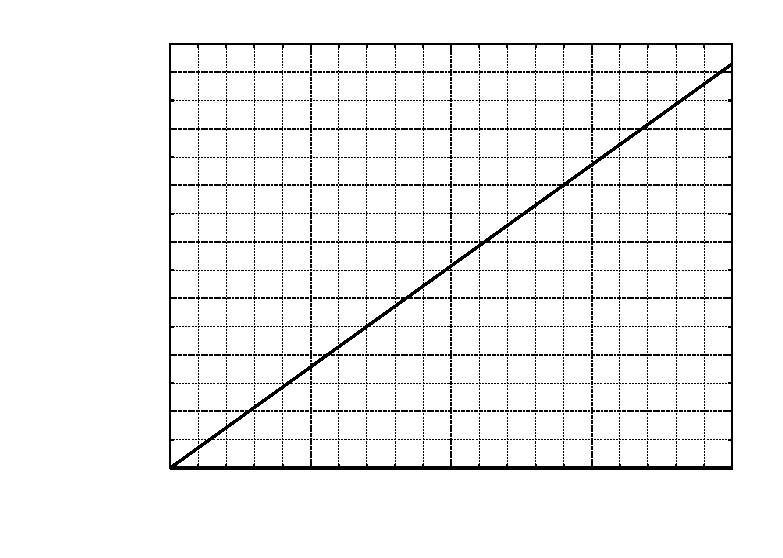
\includegraphics{../graphs/glide}}%
    \gplfronttext
  \end{picture}%
\endgroup
\end{center}  % chart from gnuplot
  \caption{Engine-Out Glide Distance}
  \end{figure}


%\textcolor{red}{Figure 3-1 Maximum Glide}

If there is sufficient altitude to attempt to restart the engine, 
the procedure is to select Boost Pump ON, switch to the other
tank (provided it has fuel), select mixture to RICH and Alternate
Air ON. Check engine gauges for an indication of cause and if no fuel
pressure is indicated change tank selection. When power is restored
and at a safe altitude, select Alternate Air to OFF and turn Boost
Pump OFF.

If engine still fails to restart and time permits, turn each ignition
OFF, then ON to isolate a potentially bad ignition system. Try moving
the throttle and/or mixture to different settings. This may restore
power if mixture is too rich or too lean or if there is a partial
fuel blockage. Try the other tank, as water in the fuel may take time
to clear the system. Allowing the engine to windmill may restore power.
If failure is due to water then fuel pressure will be normal. Empty
fuel lines may take ten seconds to refill.

\subsubsection{ROUGH RUNNING ENGINE}

A slight engine roughness during flight may be caused by carbon or lead deposits fouling one or more spark plugs. 
This may be verified by selecting one ignition system OFF at a time.  A significant power loss in single ignition
operation is evidence of either spark plug fouling or an ignition system failure.  Assuming that fouled spark plugs is
the more likely cause, set cruise power and lean the engine to the recommended cruise fuel flows for several minutes. 
If the problem does not clear up after several minutes, determine if a richer mixture setting will result in smooth
running.

A sudden engine roughness or misfiring may be evidence of an ignition problem (either magneto or electronic ignition).
 Switching one ignition system off in turn will identify which one is malfunctioning.  Select different power settings
and enrichen the mixture to determine whether continued operation on both ignition systems is possible.

If the problem continues, try different mixture and throttle settings. Select Boost Pump ON,
change fuel tanks and select Alternate Air ON. Select each ignition system
OFF then ON.

\begin{Note}[CAUTION]
The engine may quit completely when one ignition is selected OFF, if the other ignition is faulty.  
If this occurs, to prevent a severe backfire, select the mixture to ICO, wait 10 seconds, then select the ignition back ON.
Advance the mixture slowly until engine restarts.
\end{Note}

%\subsubsection{LOW FUEL PRESSURE}
%
%If fuel pressure falls, select Boost Pump ON and change fuel tanks.

\subsubsection{LOW OIL PRESSURE}

If low oil pressure is accompanied by normal oil temperature, there is a possibility that there is a leak in the line
from the engine to the oil pressure transducer manifold, or that the oil pressure relief valve has malfunctioned.  The
EIS 4000
will flash the ENGINE WARN light if the oil pressure decreases below limits. The LOW OIL PRESS light is driven by a
different transducer on the same external manifold. If only one system indicates low oil pressure it is almost certainly
a false indication.

A leak in the line to oil pressure transducer manifold is not
necessarily cause for immediate precautionary landing, as an orifice in the line will prevent sudden loss of oil from
the sump.  However the aircraft should be landed at the nearest airport for inspection.

A total loss of oil pressure accompanied by increasing oil temperature may indicate an impending total engine failure.
An off airfield landing while power is available is strongly recommended, especially in the presence of additional
indicators such as a rise in engine CHT or oil temperature, oil and/or smoke apparent. 

\subsubsection{HIGH OIL TEMPERATURE}

High oil temperature may be caused by the oil cooler door being closed
too far. High oil temperature may also be due to a low oil level,
obstruction in oil cooler (internal or external), damaged baffle seals,
a defective gauge, or other causes. The EIS 4000 ENGINE WARN light
will flash if the oil temperature becomes higher than 225\textdegree F. A steady
rise in oil temperature is a particular sign of trouble.

Always land as soon as possible at an appropriate airport/airfield
and investigate and be prepared for an engine failure. Open the oil
cooler door. Keep the airspeed up to maximize airflow over the engine.
Watch the oil pressure and CHT (Cylinder Head Temperature) gauge to
identify impending failure.

\subsection{FORCED LANDINGS}
\subsubsection{POWER OFF LANDING}

The initial action is ALWAYS TRIM FOR BEST GLIDE, 95 to 115 KIAS, depending
on weight. If engine power is not restored and time allows check for
airports/strips available and notify of problem/intent if possible.  
Select Mixture to IDLE CUT OFF.  
Closing the throttle and pulling the prop control full aft will significantly reduce windmilling drag if oil pressure
is available.  Select Fuel Selector to OFF and Ignition Switches to OFF. 
Transmit a MAYDAY.

Identify a suitable field, planning an into wind landing. Try to be
1000 ft AGL at the end of the downwind leg to make a normal landing.
Aim initially for the centre of the field (drag with a wind milling
propeller may be higher than expected) and only lower final stages
of flap when there is no doubt the field can be reached. Sideslip
as required to lose excess altitude. Plan for slowest short field
landing but above all else do not stall.

When committed to landing extend Flaps to FULL then select BATT/ALT switch to OFF. 
 Seat belts should be tight and touchdown made at the
slowest speed possible.

\textcolor{red}{Add Power-On Landing and Ditching}
\subsection{FIRES}
%\subsubsection{ENGINE FIRE DURING START}
%
%\textcolor{red}{Nothing to add to checklist?} 
%

\subsubsection{ENGINE FIRE IN FLIGHT}

The key to dealing with an engine fire is to stop the flow of fuel
to the engine compartment. Put the mixture to IDLE CUT-OFF, switch
Fuel Selector OFF, and select Boost Pump OFF. Close cabin heat and
air vents. All electrical power can be removed ahead of the firewall
by selecting the ESS BUS FEED switch to EMER (to keep the avionics powered to allow a Mayday call) and the BATT/ALT switch to OFF.

\subsubsection{ELECTRICAL FIRE}

The EFIS internal battery will power it for 3 hours (if it is fully charged), so the aircraft's entire electrical system may be 
shutdown if required due to electrical smoke or fire.  The EFIS will automatically shutdown 30 seconds
after the electrical power is cut, but the automatic shutdown sequence may be cancelled by a momentary
press of the left-most EFIS button.  The Turn Coordinator is powered from the Battery Bus, 
and will continue to be powered even if the whole electrical system is shutdown.

Fight the fire with the fire extinguisher, if required.  
Close the vents prior to using the fire extinguisher, to increase its effectiveness.
Open the vents after using the fire extinguisher to ventilate the cockpit.

%\subsubsection{CABIN FIRE}
%
%Shutdown the electrical system.  Fight the fire with the fire extinguisher, if required.  
%Close the vents prior to using the fire extinguisher, to increase its effectiveness.
%Open the vents after using the fire extinguisher to ventilate the cockpit.
%
%\subsubsection{WING FIRE}
%
%Remove electrical power to items in the wing.  Select Nav/Strobe, Landing and Taxi Lights and Pitot Heat OFF.

\subsection{OTHER}
\subsubsection{STATIC SOURCE BLOCKAGE}

If erroneous readings of the static system instruments (airspeed, altimeter and rate of climb) are suspected, the
alternate static source valve should be opened, thus supplying air to those instruments from inside the cockpit.

  \textcolor{red}{To avoid the possibility of large errors, the fresh air vents and cockpit heat should be closed. 
The maximum errors will be ????}  Adjust the altitude and airspeed readings by the corrections shown in Section
\ref{perf-sec-number}.

\subsubsection{INADVERTENT ICING ENCOUNTER}
\begin{enumerate*}
  \item Confirm pitot heat is selected ON.
  \item Turn back or change altitude to obtain an outside air temperature that is less conducive to icing.
  \item Increase RPM to minimize ice build-up on the propeller blades.
  \item Plan a landing at the nearest airport.  With extremely rapid ice build-up, select a suitable ``off-airport'' landing site.
  \item Minimize flap extension if there is an ice build-up on the horizontal stabilizer, to reduce the risk of tail plane stall.
  \item Use sideslip as required to improve forward visibility if the windscreen is obscured by ice.
  \item Increase the approach speed by at least 10 kt, to reduce the risk of wing stall.
  \end{enumerate*} 

\subsubsection{ALTERNATOR FAILURE}

Alternator failure is identified by a low voltage indication from
the EIS 4000, which will cause the ENG WARN light to flash.

The root fault may have been an over-voltage condition, in which case
the over-voltage protection system will cause the ALT CB to trip,
leading to a low voltage condition. While it is possible to put the
alternator back on line by resetting the ALT CB, this is not recommended
unless necessary for safety of flight.

The BATT/ALT switch should be selected to BATT, then BATT + ALT to attempt
to reset the alternator. If the alternator cannot be brought back
on line the Standby Alternator can be used to provide up to 8 amps
of power. Select the ESS BUS FEED to EMER, which provides power
to the Essential Bus directly from the Battery Bus, bypassing the
Battery Contactor. The Main Bus can then be shed by selecting the
BATT/ALT switch to OFF. The EFIS will continue to run using its internal
battery, however it can be restored to aircraft power by selecting
the EFIS BU switch to ON. The loads on the Essential Bus and
Battery Bus total less than 8 amps.

The following systems are unpowered in this configuration:

\begin{itemize*}
\item Boost Pump
\item Pitot Heat 
\item Landing Light 
\item Taxi Light 
\item Position Lights 
\item Strobe Lights 
\item Engine Instrument Lighting (Map light on goose neck may be used to
illuminate instrument panel) 
\item CDI Lighting 
\item Flaps 
\item Starter 
\item Wing Leveler 
\item Microair 760 Com (COM 2) 
\item Intercom 
\item Low Oil Pressure Warning Light 
\item Analog Tach and MP
\item Defrost Fan
\end{itemize*}
The BATT/ALT switch may be selected to ON prior to landing to restore
power to all systems.

\subsubsection{STARTER ENGAGED LIGHT ILLUMINATED}
The STARTER ENGAGED caution light illuminates whenever the starter is engaged.  If this light remains illuminated after
the starter switch has been released, it indicates that the starter relay is stuck closed, and the starter is still
powered.
 Continuing to supply power to the
starter will eventually result in complete loss of electrical system power, substantial starter damage, and possible
damage to other electrical system components.  If the starter is stuck closed, the only way to remove power from the
starter is to select the BATT/ALT switch to OFF.


\subsubsection{WING-LEVELER MALFUNCTION}

Press the red Wing-Leveler/Trim Disconnect button on the control stick, and hold it.  This removes power from the servo, and should cause it to release.
Select the Wing-Leveler Power switch OFF (RH console), then release the Wing-Leveler/Trim Disconnect button.  
%If required, the control rod from the servo to the controls may be disconnected by pulling the ``pip'' pin located at the base of the front control stick, between the stick and the front spar area.

\subsubsection{RUNAWAY TRIM}

Press the red Wing-Leveler/Trim Disconnect button on the control stick, and hold it.  Select the Trim Power switch OFF (RH console), then release the Wing-Leveler/Trim Disconnect button.

\subsubsection{HIGH CO}

Decrease power.  Set mixture well lean of peak (stops CO production).  Close both cabin heat controls.  Open the vents.  Monitor the CO Monitor readings.  
Immediate action is required if the red light is illuminated.  
Consider slowing the aircraft and cracking the canopy open if there is not an immediate decrease in the CO levels.

\subsubsection{LANDING WITH NO ELEVATOR CONTROL}
\textcolor{red}{Add this item after in-flight assessment}

\subsubsection{SPIN RECOVERY}

Upright spin - The upright spin recovery procedure is:
\begin{enumerate*}
  \item Retard throttle to idle.
  \item Retract flaps, if extended.
  \item Place ailerons to neutral position.
  \item Apply and hold full rudder opposite to spin direction.  If the visibility of the ground does not allow the spin direction to be determined, use the turn needle --- depress the rudder on the opposite side to that of the turn needle.
  \item Just after the rudder reaches the stop, move the stick briskly forward far enough to break the stall.
  \item Hold these control inputs until rotation stops.  Premature relaxation of the recovery control inputs may prevent spin recovery.
  \item As rotation stops, neutralize the rudder, and recover from the dive, using g as required to stay below $V_{NE}$ without exceeding the load factor limit.  Aggressive use of g early in the recovery will minimize the airspeed build-up.
  \end{enumerate*}
  
\begin{Note}
The inverted spin recovery procedure has not been validated via flight test.
\end{Note}

Inverted spin - The inverted spin recovery procedure is:
\begin{enumerate*}
  \item Retard throttle to idle.
  \item Retract flaps, if extended.
  \item Place ailerons to neutral position.
  \item Confirm spin direction by reference to the turn needle --- the turn needle moves to the side of the spin direction.  Apply and hold full rudder opposite to spin direction.  
  \item Just after the rudder reaches the stop, move the stick briskly \textbf{aft} far enough to break the stall.
  \item Hold these control inputs until rotation stops.  Premature relaxation of the recovery control inputs may prevent spin recovery.
  \item As rotation stops, neutralize the rudder, and recover from the dive, using g as required to stay below $V_{NE}$ without exceeding the load factor limit.  Aggressive use of g early in the recovery will minimize the airspeed build-up.
  \end{enumerate*}

% !iTeXMac(input): POH.tex
\chapter{NORMAL PROCEDURES}
\vspace{\minitocspacebefore}
\minitoc
\cleardoublepage

\section{GENERAL}

Pilots should familiarize themselves with the procedures in this section
to become proficient with the normal safe operation of the aircraft.

\section{AIRSPEEDS FOR NORMAL OPERATION}
(\textcolor{red}{Red text indicates provisional information, based
on the RV-8A Aircraft Performance Report published by the CAFE Foundation}.)

\begin{center}\begin{tabular}{llr}
$\mathrm{V_{R}}$&
Takeoff rotate speed&
60\tabularnewline
&
Normal Takeoff, speed at 50 ft &
\textcolor{red}{70}\tabularnewline
&
Short Field Takeoff, speed at 50 ft&
\textcolor{red}{TDB}\tabularnewline
$\mathrm{V_{Y}}$ &
Best rate of climb speed, Sea Level&
102 KIAS\tabularnewline
$\mathrm{V_{X}}$ &
Best angle of climb speed, Sea Level&
65 KIAS\tabularnewline
$\mathrm{V_{BG}}$&
Best glide angle&
115 KIAS\tabularnewline
$\mathrm{V_{A}}$ &
Manoeuvring speed&
\textcolor{red}{120} KIAS\tabularnewline
$\mathrm{V_{S_{0}}}$ &
Stall Full Flap&
\textcolor{red}{51} KIAS\tabularnewline
$\mathrm{V_{S}}$ &
Stall Flaps UP&
\textcolor{red}{65} KIAS\tabularnewline
$\mathrm{V_{FE}}$ &
Maximum speed with flaps extended &
\textcolor{red}{87} KIAS\tabularnewline
$\mathrm{V_{REF}}$ &
Final approach speed (full flap)&
70\tabularnewline
$\mathrm{V_{REF0}}$ &
Final approach speed (zero flap)&
80\tabularnewline
&
Demonstrated crosswind velocity&
\textcolor{red}{12}\tabularnewline
\end{tabular}\end{center}

%\addpenalty{-10000}
%\section{ENGINE OPERATING CONDITIONS}
%
%\begin{center}\begin{tabular}{lccccc}
%&
%RPM&
%HP&
%GPH&
%Max Oil Consumption&
%Max. CHT\tabularnewline
%&
%&
%&
%&
%(Qts/Hr)&
%(deg C)\tabularnewline
%Normal Rated&
%2700&
%200&
%--&
%.89&
%260\tabularnewline
%Performance Cruise (75\%)&
%2450&
%150&
%12.3&
%.5&
%260\tabularnewline
%Economy Cruise (65\%)&
%2350&
%130&
%9.5&
%.44&
%260\tabularnewline
%\end{tabular}\end{center}

\cleardoublepage
% !iTeXMac(input): POH.tex
%\section*{NORMAL CHECKLISTS} % leave this line commented out, 
%as it destroys the visual flow of the checklist page.
% Find a way to get "NORMAL CHECKLIST" in the header instead.
%\addcontentsline{toc}{section}{\numberline {NCL}Normal Checklist}
\changepage{\checklistTextHeight}{\checklistTextWidth}{\checklistEvenSideMargin}{\checklistOddSideMargin}{}{\checklistTopMargin}{0pt}{0pt}{0pt}% original settings, with no room for header or footer

%\addcontentsline{toc}{section}{\numberline { }NORMAL CHECKLIST}
\addcontentsline{toc}{section}{NORMAL CHECKLIST}
%\ohead{NORMAL CHECKLIST}% puts "NORMAL CHECKLIST" in the header.
\chead{\Large NORMAL CHECKLIST} % puts "NORMAL CHECKLIST" in the header.
% \ohead{DRAFT --- \thistime \ \cdndate\today}
\ohead{Created --- \thistime \ \cdndate\today}

\begin{multicols}{2}
% \raggedcolumns

\subsection*{PREFLIGHT INSPECTION }

\subsubsection*{COCKPIT}
\begin{enumerate*}
\item Ignition Switches\dotfill OFF
\item BATT/ALT \dotfill BATT
\item Fuel Gauges \dotfill CHECK
\item Fuel Selector \dotfill LOWEST TANK
\item Landing \& Taxi Lights \dotfill CHECK A/R
\item Flaps \dotfill EXTEND
\item BATT/ALT \dotfill OFF
\item Alternate Static Source Hose \dotfill SECURE
\item Rear Stick \dotfill A/R 
\item Rear Seat Belts \dotfill A/R
\item Rear Cockpit Side Pockets \dotfill A/R
\item ELT Antenna \dotfill SECURE
\item Rear Baggage Area \dotfill SECURE
\item ELT \dotfill ARM
\end{enumerate*}

\subsubsection*{LEFT WING }
\begin{enumerate*}
\item Flap Pushrod End \dotfill SECURE
\item Aileron Pushrod \dotfill SECURE
\item Aileron Hinge \dotfill SECURE
\item Nav Light Cover \dotfill SECURE
\item Taxi Light \dotfill SECURE
\item Pitot Tube \dotfill CLEAR
\item Fuel Quantity \dotfill VISUAL CHECK
\item Fuel Tank Drain \dotfill $\mathrm{H_{2}O}$ CHECK
\item Gascolator Drain \dotfill $\mathrm{H_{2}O}$ CHECK
\end{enumerate*}

\subsubsection*{FORWARD FUSELAGE }
\begin{enumerate*}
\item L Tire \& Wheel Pant \dotfill CHECK COM
\item Antenna \dotfill SECURE
\item Fuel vents \dotfill CLEAR
\item Exhaust Pipes \dotfill SHAKE ENDS
\item Cowl \dotfill SECURE
\item Air Inlets \dotfill CLEAR
\item Air Filter \dotfill CHECK
\item Spinner \dotfill SECURE
\item Prop \dotfill CHECK
\item Oil Quantity \dotfill CHECK 
\item Oil Door \dotfill SECURE
\item Fwd Baggage \dotfill ITEMS CHECK
\item Windshield \dotfill CLEAN
\item Transponder Antenna \dotfill SECURE
\item R Tire \& Wheel Pant \dotfill CHECK
\end{enumerate*}

\subsubsection*{RIGHT WING }
\begin{enumerate*}
\item Fuel Tank Drain \dotfill $\mathrm{H_{2}O}$ CHECK 
\item Fuel Quantity \dotfill VISUAL CHECK
\item Landing Light \dotfill SECURE
\item Nav Light Cover \dotfill SECURE
\item Aileron Hinge \dotfill SECURE
\item Aileron Pushrod \dotfill SECURE
\item Flap Pushrod End \dotfill SECURE
\end{enumerate*}

\subsubsection*{RIGHT REAR FUSELAGE }
\begin{enumerate*}
\item GPS Antenna \dotfill SECURE
\item Canopy \dotfill CHECK
\item Static Port \dotfill CLEAR
\end{enumerate*}

\subsubsection*{EMPENNAGE}
\begin{enumerate*}
\item Empennage Fairing Top \dotfill SECURE
\item Empennage Fairing Bottom \dotfill SECURE
%\item Empennage Fairing \dotfill Secure round elevator
\item Empennage Fairing \dotfill SECURE AROUND ELEV.
\end{enumerate*}

\subsubsection*{LEFT REAR FUSELAGE}
\begin{enumerate*}
\item Static Port \dotfill CLEAR
\item Canopy \dotfill CHECK
\end{enumerate*}
\end{multicols} % end multicols so that the "This page intentionally left blank" will go in center of page.
\cleardoublepage

\begin{multicols}{2}
\raggedcolumns
\subsection*{IN-FLIGHT CHECKLISTS}

\subsubsection*{BEFORE START}
\begin{enumerate*}
\item Seat Belts \dotfill SECURE
\item Controls \dotfill FREE \& CORRECT
\item Throttle \dotfill FULL OPEN
\item Prop \dotfill LO RPM
\item Mixture \dotfill ICO
\item Alternate Air \dotfill CLOSED
\item Oil Cooler Door \dotfill A/R
% \item CO Monitor \dotfill OFF
\item Ignition Switches \dotfill OFF
% \item Inst Panel Switches \dotfill OFF
\item All Switches and Avionics \dotfill OFF or NORM
% \item Avionics \dotfill OFF
% \item RH Console Switches \dotfill OFF or NORM
\item ESS BUS FEED \dotfill EMER
\item ENG INST \dotfill ON
\item TRIM \dotfill FRONT or FRONT + REAR
\item Trim \dotfill CHECK
\item Trim Cut-out \dotfill CHECK
\item EIS 4000 \dotfill ENTER FUEL QTY
%\item COM 2 \dotfill ON
%\item ATIS/Clearance \dotfill OBTAIN
%\item Altimeter \dotfill SET
\item BATT/ALT \dotfill BATT + ALT
\item ESS BUS FEED \dotfill NORM
\item Engine Warn Light \dotfill CHECK ON
\item Oil Press Light \dotfill CHECK ON
\item Nav Lights \dotfill A/R
% \item Intercom \dotfill CHECK
\end{enumerate*}

\subsubsection*{ENGINE START (Cold /Warm)}
\begin{enumerate*}
% \item Seat Belts \dotfill SECURE
% \item Controls \dotfill FREE \& CORRECT
% \item Canopy \dotfill A/R
\item Fuel Selector \dotfill LEFT or RIGHT
% \item Strobe\dotfill A/R
\item IGNITION, MAG \dotfill ON
\item Starter Switch \dotfill ENABLE
%\item Throttle \dotfill FULL OPEN
%\item Mixture \dotfill ICO
\item Boost Pump \dotfill ON
\item Mixture \raggedright \dotfill FULL RICH 4-5 SEC - COLD\\\dotfill FULL RICH 2-3 SEC WARM
% \item Mixture \raggedright \dotfill FULL RICH 5 SEC - COLD\\\hfill FULL RICH 2-3 SEC - WARM
\item Mixture \dotfill ICO
\item Boost Pump \dotfill OFF
\item Throttle \dotfill 1/2" OPEN
\item Call \dotfill CLEAR
\item Starter \dotfill ENGAGE
\item IGNITION, ELEC \dotfill ON (after two blades)
\suspend{enumerate*}
\begin{Note}[CAUTION]
Do not select Electronic Ignition ON until the engine
has turned two blades. Failure to observe this restriction may result
in engine kick-back and starter damage.
%Do not select EI ON prior to starter engagement. The EI may
%be selected ON while the starter is engaged, as long as the engine
%has turned two blades. Failure to observe this restriction may result
%in engine kick-back and starter damage.
\end{Note}
\resume{enumerate*}
\item Mixture \dotfill RICH WHEN ENG FIRES
\item Engine \dotfill 1000 RPM
\item Oil Pressure \dotfill CHECK (30 s)
\end{enumerate*}

\subsubsection*{ENGINE START (Hot)}
\begin{enumerate*}
% \item Seat Belts \dotfill SECURE
% \item Controls \dotfill FREE \& CORRECT
% \item Canopy \dotfill A/R
\item Fuel Selector \dotfill LEFT or RIGHT
% \item Strobe \dotfill ON
\item IGNITION, MAG \dotfill ON
\item Starter Switch \dotfill ENABLE
%\item Throttle \dotfill FULL OPEN
\item Mixture \dotfill ICO
\item Boost Pump \dotfill ON
\item Call \dotfill CLEAR
\item Starter \dotfill ENGAGE
\item IGNITION, ELEC \dotfill ON (after two blades)
\suspend{enumerate*}
\begin{Note}[CAUTION]
Do not select Electronic Ignition ON until the engine
has turned two blades. Failure to observe this restriction may result
in engine kick-back and starter damage.
%Do not select EI ON prior to starter engagement. The EI may
%be selected ON while the starter is engaged, as long as the engine
%has turned two blades. Failure to observe this restriction may result
%in engine kick-back and starter damage.
\end{Note}
\resume{enumerate*}
\item Mixture \dotfill RICH WHEN ENG FIRES
\item Throttle \dotfill RETARD
\item Engine \dotfill 1000 RPM
\item Oil Pressure \dotfill CHECK (30 s)
\item Boost Pump \dotfill OFF
\end{enumerate*}

\subsubsection*{AFTER START}
\begin{enumerate*}
\item OIL PRESS Light\dotfill OUT
\item STARTER ENGAGED Light \dotfill OUT
\item STARTER Switch\dotfill OFF \& Guarded
\item FLAPS \dotfill UP
\item Voltage \dotfill CHECK
\item Fuel Pressure \dotfill CHECK
%\item GNS 430 \dotfill ON
%\item Transponder \dotfill STBY, CODE SET
%\item COM 2 \dotfill ON
%\item Narco 122D \dotfill ON
\item Avionics \dotfill ON
\item TURN COORD \dotfill ON
\item WING LVLR \dotfill ON
\item CO Monitor Self Test \dotfill CHECK
\item ATIS/Clearance \dotfill OBTAIN
\item Altimeter \dotfill SET
%\item GNS 430 \dotfill ENTER FPLAN
\end{enumerate*}

\subsubsection*{TAXI}
\begin{enumerate*}
% \item TAXI LT \dotfill ON
\item Brakes \dotfill CHECK
\item Flight Instruments \dotfill CHECK
\item \emph{For IFR or Night Operations ...}
\begin{itemize*}
\item Autopilot Override \dotfill CHECK
\end{itemize*}
\end{enumerate*}

\subsubsection*{RUNUP}
\begin{enumerate*}
\item Fuel Selector \dotfill CHANGE TANKS
\item Mixture \dotfill RICH
\item Throttle \dotfill 1800 RPM
\item Prop \dotfill CYCLE
\item IGNITION, ELEC \dotfill OFF/ON
\item IGNITION, MAG \dotfill OFF/ON
\item \emph{For IFR or Night Operations ...}
\begin{itemize*}
\item ESS BUS FEED \dotfill EMER
\item BATT/ALT \dotfill OFF
\item STBY ALT \dotfill ON
\item Voltage \dotfill CHECK
\item STBY ALT \dotfill OFF
\item BATT/ALT \dotfill BATT + ALT
\item ESS BUS FEED \dotfill NORM
\end{itemize*}
\item Voltage \dotfill CHECK
\item Throttle \dotfill IDLE CHECK
\item Mixture \dotfill LEAN
\end{enumerate*}

\columnbreak % added to force all of runup checklist onto one page

\subsubsection*{BEFORE TAKEOFF}
\begin{enumerate*}
%\item SPOT \dotfill TRACK MODE
\item Seat Belts \dotfill SECURE
\item Flight Controls \dotfill FREE
\item Trims \dotfill SET
\item Flaps \dotfill SET
\item Prop \dotfill FULL FWD
\item Ignition Switches\dotfill BOTH ON
\item Alternate Air \dotfill CLOSED
\item Oil Cooler Door \dotfill A/R
\item Radios/Navaids \dotfill SET
\item Transponder \dotfill CODE SET + ALT
%\item Wing Leveler \dotfill TC
\item Altimeter \dotfill SET/CHECK
\item Engine Instruments \dotfill CHECK
\item MSTR WARN Light \dotfill OUT
% \item Fuel \dotfill CHECK
\item Fuel Selector \dotfill FULLEST TANK
\item T/O Brief \dotfill COMPLETE\vspace{0.5ex}
\hrule width \columnwidth \vspace{1ex}
\item Canopy \dotfill LATCHED
\item PITOT HEAT \dotfill A/R
\item LDG LT \& TAXI LT \dotfill ON or FLASH
\item NAV/STR \dotfill NAV + STR
\item Mixture \dotfill RICH
\item Boost Pump \dotfill ON
\item Compasses \dotfill CHECK
\end{enumerate*}

\subsubsection*{AFTER TAKEOFF}
\begin{enumerate*}
\item Flaps \dotfill UP
\item LDG LT \& TAXI LT \dotfill A/R
% \item Transponder \dotfill CONFIRM ALT
\item Boost Pump \dotfill OFF
\item Power \dotfill 2500 rpm/Full Throttle
\end{enumerate*}

\subsubsection*{CRUISE}
\begin{enumerate*}
\item Power \dotfill SET
\item Mixture \dotfill SET
\item Fuel \dotfill CHECK
\item Oil Cooler Door \dotfill A/R
% \item Fuel Selector \dotfill CHANGE TANKS EVERY 30 MN
\end{enumerate*}

\columnbreak
\subsubsection*{AEROBATICS}
\begin{enumerate*}
\item Fuel \dotfill LEFT TANK
\item Mixture \dotfill RICH
\item Harness \dotfill TIGHT
\item Loose Items \dotfill STOW
\item Area \dotfill CLEAR
\end{enumerate*}

\subsubsection*{DESCENT}
\begin{enumerate*}
\item Parking Brake \dotfill OFF
\item Altimeter \dotfill SET
\item Approach \dotfill BRIEF
\item Oil Cooler Door \dotfill A/R
\item LDG LT \& TAXI LT \dotfill A/R
\end{enumerate*}

\subsubsection*{BEFORE LANDING}
\begin{enumerate*}
\item Seat Belts \dotfill SECURE
\item Fuel Selector \dotfill FULLEST TANK
\item Mixture \dotfill RICH
\item Boost Pump \dotfill ON
% \item Wing Leveler \dotfill TC
\item Prop \dotfill FULL FWD
\item Flaps \dotfill A/R
% \item LDG LT \& TAXI LT \dotfill A/R
% \item Airspeed \dotfill XX KT
\end{enumerate*}

\subsubsection*{AFTER LANDING}
\begin{enumerate*}
\item PITOT HEAT \dotfill OFF
\item Mixture \dotfill LEAN
\item Oil Cooler Door \dotfill OPEN
\item Boost Pump \dotfill OFF
% \item Flaps \dotfill UP
% \item NAV/STR \dotfill OFF or NAV
% \item TAXI LT \dotfill A/R
% \item LDG LT \dotfill OFF
\item External Lights \dotfill A/R
\item Transponder \dotfill STBY
\item Flaps \dotfill 90\% DOWN
\end{enumerate*}

\subsubsection*{SHUTDOWN}
\begin{enumerate*}
\item Avionics \dotfill OFF
% \item ENG INST \dotfill OFF
% \item TURN COORD \dotfill OFF
% \item DFRST FAN \dotfill OFF
% \item TRIM \dotfill OFF
% \item WING LVLR \dotfill OFF
\item Throttle \dotfill IDLE
\item Dead Mag \dotfill CHECK
\item Mixture \dotfill ICO
\item Ignition Switches \dotfill BOTH OFF
\item Fuel Selector \dotfill OFF
% \item NAV/STR \dotfill OFF
\item All Switches \dotfill OFF or NORM
%\item SPOT \dotfill OFF
%\item BATT/ALT \dotfill OFF
\end{enumerate*}
\end{multicols}

\cleardoublepage
\ohead{\leftmark} % put Section name back in outer header
\chead{} % remove center header
\changepage{\checklistTextHeight*-1}{\checklistTextWidth*-1}{\checklistEvenSideMargin*-1}{\checklistOddSideMargin*-1}{}{\checklistTopMargin*-1}{0pt}{0pt}{0pt}% original settings, with no room for header or footer



\cleardoublepage
\changepage{\checklistTextHeight}{\checklistTextWidth}{\checklistEvenSideMargin}{\checklistOddSideMargin}{}{\checklistTopMargin}{0pt}{0pt}{0pt}% original settings, with no room for header or footer

%\addcontentsline{toc}{section}{\numberline { }NORMAL CHECKLIST}
\addcontentsline{toc}{section}{CHEAT SHEET}
%\ohead{NORMAL CHECKLIST}% puts "NORMAL CHECKLIST" in the header.
\chead{\Large CHEAT SHEET} % puts "NORMAL CHECKLIST" in the header.
% \ohead{DRAFT --- \thistime \ \cdndate\today}
\ohead{Created --- \thistime \ \cdndate\today}

\begin{multicols}{2}
\raggedcolumns

\subsection*{EIS 4000}
\subsubsection*{CHANGE FUEL QUANTITY TO FULL FUEL}
\begin{enumerate*}
\item L and R Buttons\dotfill PRESS AND HOLD
\item INC and DEC Soft Keys\dotfill PRESS (to set 42 USG)
\item NEXT Soft Key\dotfill PRESS (to return to normal display)
\end{enumerate*}

\subsubsection*{CHANGE FUEL QUANTITY TO ANY VALUE}
\begin{enumerate*}
\item L and R Buttons\dotfill PRESS AND HOLD
\item INC or DEC Soft Keys\dotfill PRESS (to set desired quantity)
\item NEXT Soft Key\dotfill PRESS (to return to normal display)
\end{enumerate*}

\subsubsection*{SET ALARM LIMITS}
\begin{enumerate*}
\item L and C Buttons\dotfill PRESS AND HOLD FOR 10S
\item UP or DOWN Soft Keys\dotfill PRESS (to modify parametres)
\item NEXT Soft Key\dotfill PRESS (to advance to next parametre)
\item NEXT Soft Key\dotfill PRESS REPEATEDLY (to return to normal display)
\end{enumerate*}

\subsubsection*{ACCESS CONFIGURATION MENUS}
\begin{enumerate*}
\item C and R Buttons\dotfill PRESS AND HOLD FOR 10S
\item UP or DOWN Soft Keys\dotfill PRESS (to modify parametres)
\item NEXT Soft Key\dotfill PRESS (to advance to next parametre)
\item EIS Power\dotfill OFF-ON (to return to normal display)
\end{enumerate*}

\subsubsection*{LEANING MODE}
\begin{enumerate*}
\item Centre and R Buttons\dotfill PRESS AND HOLD
\end{enumerate*}


\columnbreak % added to force all of GNS 430W stuff onto one page
\subsection*{GNS 430W}
\subsubsection*{REVIEW FLT PLAN LATS \& LONGS}
\begin{enumerate*}
\item FPL Page\dotfill SELECT
\item Cursor\dotfill ACTIVATE
\item Waypoint Name\dotfill SELECT
\item ENT Button\dotfill PUSH (to see wpt info)
\item Lat/Long\dotfill REVIEW
\item ENT Button\dotfill PUSH (to move to next wpt)
\end{enumerate*}

\subsection*{SPOT}
\subsubsection*{START TRACKING}
\begin{enumerate*}
\item Power Button\dotfill PRESS AND HOLD (until lights flash)
\item Footprint Button\dotfill PRESS AND HOLD (until light flashes)
\end{enumerate*}

\subsubsection*{SEND CHECK-IN MESSAGE}
\begin{enumerate*}
\item Power Button\dotfill PRESS AND HOLD (until lights flash)
\item Checkmark/OK Button\dotfill PRESS AND HOLD (until light flashes)
\end{enumerate*}

\subsubsection*{SEND CUSTOM MESSAGE}
\begin{enumerate*}
\item Power Button\dotfill PRESS AND HOLD (until lights flash)
\item Text Bubble Button\dotfill PRESS AND HOLD (until light flashes)
\end{enumerate*}

\subsubsection*{SEND REQUEST FOR ASSISTANCE (non life threatening)}
\begin{enumerate*}
\item Power Button\dotfill PRESS AND HOLD (until lights flash)
\item Holding Hands Button\dotfill PRESS AND HOLD (until light flashes)
\end{enumerate*}

\subsubsection*{SEND EMERGENCY REQUEST FOR ASSISTANCE}
\begin{enumerate*}
\item Power Button\dotfill PRESS AND HOLD (until lights flash)
\item SOS Button\dotfill LIFT TAB
\item SOS Button\dotfill PRESS AND HOLD (until light flashes)
\end{enumerate*}

\subsubsection*{CANCEL EMERGENCY REQUEST FOR ASSISTANCE}
\begin{enumerate*}
\item Power Button\dotfill PRESS AND HOLD (until lights flash)
\item SOS Button\dotfill LIFT TAB
\item SOS Button\dotfill PRESS AND HOLD (until light flashes red)
\item SPOT\dotfill LEAVE POWERED (until SOS button stops flashing red)
\end{enumerate*}

\end{multicols}

\cleardoublepage
\ohead{\leftmark} % put Section name back in outer header
\chead{} % remove center header
\changepage{\checklistTextHeight*-1}{\checklistTextWidth*-1}{\checklistEvenSideMargin*-1}{\checklistOddSideMargin*-1}{}{\checklistTopMargin*-1}{0pt}{0pt}{0pt}% original settings, with no room for header or footer


\section{AMPLIFIED PROCEDURES}

\subsection{PREFLIGHT INSPECTION}
The following items should receive particular emphasis during the preflight inspection.

\textbf{Propeller} --- Check the amount of free play in the propeller blades, moving the blade tips in the plane of rotation. 1/8\char`\"{} of free play is acceptable. 2 degrees of blade rotation angle free play is acceptable. Check that the stainless steel erosion strips on the outer portion of the blade leading edges is secure. The inner PU-strip self-adhesive shield may be missing, but should be replaced within 10 hours.

Check the fibreglass blade covers for cracks. Cracks along the leading edge and at the edge of the erosion shield are acceptable, as long as the erosion shield is not loose. Cracks in the painted surface are acceptable, as long as no moisture can enter the wooden blade core. Blisters or delaminations up to one square inch are acceptable. Cracks in the stainless steel erosion shield require immediate repair.

\textbf{Fuel Tank Vents} --- The fuel vent plugs are easily missed, as the fuel vents are below the forward fuselage. Ensure that they are removed.

\textbf{Flaps}
\begin{Note}[CAUTION]
With the flaps fully extended, there is a risk that someone standing behind the wing could press on flap trailing edge, and force the flaps to move far enough that the forward edge of the upper flap skin could move aft of the aft edge of the upper wing skin. If this condition is not detected significant flap and/or upper wing skin damage may occur when the flaps are retracted. During the preflight inspection, carefully inspect the transition between the upper wing skin and the flaps to confirm that the forward edge of the upper flap skin has not come out from under the aft edge of the upper wing skin. When boarding the aircraft after the preflight inspection, be careful not to push forward on the trailing edge of the flap. 

The risk of forcing the flaps far enough to trigger this issue is mitigated by slightly retracting the flaps after landing.
\end{Note}


\textbf{Tires} --- The tires are almost completely hidden beneath the wheel pants, so it can be difficult to see if the tire pressure is low. Carefully check the clearance between the tire sidewalls and the wheel pant openings.

\textbf{Pitot-Static System} --- Ensure that the pitot cover is removed from the pitot tube, which is hidden beneath the left wing. The static system hose connected to the alternate static valve is easily knocked loose (mounted on the side of the right landing gear box in the cockpit). Check it for security, and be careful not to knock that area with the feet.

\subsection{COCKPIT ENTRY AND EGRESS}
\textbf{Front Seat Entry} --- Stand on the left wing walk area. 
% Place a towel on the front seat cushion. Place the right foot on the seat cushion. 
Place the right foot on the gold coloured wing spar centre section to the right of the front seat cushion. Support the weight of the upper body by placing the hands on the sides of the cockpit, or on the tubular structure behind the front seat back. Place the left foot on the cockpit floor ahead of the seat cushion.

\textbf{Rear Seat Entry} --- Stand on the left wing walk area. Place a towel on the rear seat cushion. Hang onto the tubular framework just behind the front seat back. Place the right foot on the seat cushion. Place the left foot on the floor ahead of the seat. Place the left hand on the canopy rail. Place the right foot on the floor ahead of the seat. Sit down.

\begin{Note}[CAUTIONS]
  \textbf{Flaps} --- Extend the flaps 90\% for cockpit entry and egress, to ensure that the flaps are not stepped upon.
  
  \textbf{Front Seat} --- Do not use the edge of the windscreen as a handhold when entering or exiting the cockpit. The windscreen fairing that extends past the edge of the
windscreen may be damaged if it is subjected to too much force. Be careful to not kick the intercom system volume knobs on the lower edge of the instrument panel with the feet. Be careful to not kick the alternate static valve on the inboard side of the right landing gear box.

  \textbf{Rear Seat} --- Warn all passengers to be careful not to lean back against the sliding canopy when they enter or leave the aircraft.
  \end{Note}
  
\subsection{STARTING ENGINE}
%follow paragraphs slavishly lifted from the Cessna 177RG POH, as it has a similar engine model.
In cold weather, the engine compartment temperature falls rapidly following engine shutdown, and the injector nozzle lines remain nearly full of fuel. Cold weather starting procedures are therefore relatively simple, with highly predictable results. However, in extremely hot weather, engine compartment temperatures increase rapidly following engine shutdown, and fuel in the lines will vapourize and escape into the intake manifold.

Hot weather starting procedures depend considerably on how soon the next engine start is attempted. Within the first \textcolor{red}{20 to 30 minutes} after shutdown, the fuel manifold is adequately primed, and the empty injector nozzle lines will fill before the engine dies. However, after approximately \textcolor{red}{30 minutes}, the vapourized fuel in the manifold will have nearly dissipated, and some slight ``priming'' could be required to refill the nozzle lines and keep the engine running after the initial start. Starting a hot engine is facilitated by advancing the mixture control promptly to one third open when the engine fires, and then smoothly to full rich as power develops.

Should the engine tend to die after starting, temporarily select the boost pump ON and adjust throttle as necessary to keep the engine running.

In the event of over-priming or flooding, select the boost pump OFF, open the throttle from one half to full open, and continue cranking with the mixture at CUT-OFF. When the engine fires, smoothly advance the mixture control to FULL RICH and retard the throttle to the desired idle speed.

If the engine is under-primed (most likely in cold weather with a cold engine) it will not fire at all, and additional priming will be necessary.

After starting, if the oil pressure gauge does not begin to show oil pressure within 30 seconds in the summertime, and 60 seconds in very cold weather, stop the engine and investigate.

\begin{Note}
  Additional details concerning cold weather starting and operation may be found under COLD WEATHER OPERATION
  paragraphs in this section.
  \end{Note}

\subsection{TAXIING}
\subsubsection{AUTOPILOT}
\textbf{Pre-Flight Test} --- A preflight override and disengagement test should be conducted if the autopilot is to be used in IMC or at night. 

\begin{enumerate}
  \item WING LVLR --- ON (Right Console)
%  \item TURN knob --- Centre
  \item Autopilot --- ON
  \item H~NAV and V~NAV --- Engage
  % \item TK$\bullet$TC$\bullet$WL Switch --- WL. Engages Wing-Leveler mode.
  % \item Make left and right turns during taxi --- Stick should move against the turn.
  \item Controls --- Override. Confirm that the autopilot servo clutches will slip to allow the stick to be moved in both axis when the autopilot is engaged.
  \item Trim/Wing-Leveler Disconnect Switch on control stick --- Press and Release. Confirm both servos release while disconnect switch is pressed. Release the Disconnect switch.
  % \item TK$\bullet$TC$\bullet$WL Switch --- TC. Selects Turn Coordinator mode, disengaging the wing-leveler servo from the flight controls.
  \end{enumerate}

\needspace{15\baselineskip}
  \subsubsection{CONTROL USE DURING TAXIING}
When taxiing, it is important that aileron and elevator be used as appropriate to the wind direction (see Figure \ref{taxi-diagram}. Taxiing over loose gravel should only be done at low engine speed to avoid abrasion and stone damage to propeller tips.
\begin{figure}[htb]
  \begin{center}
  \begin{overpic}[bb=0 0 336 330]{../Diagrams/taxi}
    \newsavebox{\windarrow}
    \newsavebox{\windarroww}
%    \savebox{\windarrow}(10,10){\Line(5,0)}
%    \savebox{\windarrow}(10,10){\drawline(0,0)(5,0)(5,5)(6,5)(2.5,7.5)(-1,5)(0,5)(0,0)}
    \savebox{\windarrow}(10,10){\drawline(0,0)(7,0)(7,-1)(9.5,2.5)(7,6)(7,5)(0,5)(0,0)\put(0.3,1.4){WIND}}
    \savebox{\windarroww}(10,10){\drawline(0,0)(-7,0)(-7,-1)(-9.5,2.5)(-7,6)(-7,5)(0,5)(0,0)\put(-8.4,1.4){WIND}}
%    \arrowlength{12pt}
    \put(5,90){\rotatebox{315}{\usebox{\windarrow}}}
    \put(76,83){\rotatebox{45}{\usebox{\windarroww}}}
    \put(5,7.5){\rotatebox{45}{\usebox{\windarrow}}}
    \put(76,14){\rotatebox{315}{\usebox{\windarroww}}}
    \put(8,70){\begin{boxedminipage}[b]{1.3in}\small \centering USE AFT STICK AND LEFT AILERON\end{boxedminipage}}
    \put(60,70){\begin{boxedminipage}[b]{1.3in}\small \centering USE AFT STICK AND RIGHT AILERON\end{boxedminipage}}
    \put(8,37.5){\begin{boxedminipage}[t]{1.3in}\small \centering USE FORWARD STICK AND RIGHT AILERON\end{boxedminipage}}
    \put(60,37.5){\begin{boxedminipage}[t]{1.3in}\small \centering USE FORWARD STICK AND LEFT AILERON\end{boxedminipage}}
    \end{overpic}
    \end{center}

%  \textcolor{red}{Add diagram of stick position vs wind while taxiing.}
  \caption{Control Use During Taxiing}
  \label{taxi-diagram}
  \end{figure}

\subsection{BEFORE TAKEOFF}
  \subsubsection{WARM-UP}
  Since the engine is closely cowled, care should be taken to avoid over-heating during prolonged engine operation on the ground. Long periods of idling at low RPM may caused fouled spark plugs. It is advisable to lean aggressively while at low power on the ground. If the mixture is leaned, it must be leaned far enough that the engine would run noticeably rough during the higher power setting of the ignition check.
  
  \subsubsection{IGNITION CHECK}
  The ignition check should be done at 1800 RPM as follow:
  \ifthenelse{\thePMAG = 0}{
  \begin{enumerate}
  \item Select the IGNITION, MAG switch to OFF. There should be no RPM drop, as the electronic ignition is more advanced than the magneto at this condition, so the spark from the magneto contributes little. The engine should run smoothly on the electronic ignition.
  \item Select the IGNITION, MAG switch to ON.
  \item Select the IGNITION, ELEC switch to OFF. The RPM drop should be approximately 100 RPM, and the engine should run smoothly on the magneto. 
  \item Select the IGNITION, ELEC switch to ON.
  \end{enumerate}
  }{
  \begin{enumerate}
  \item Select the IGNITION, MAG switch to OFF. There should be approximately 20 rpm drop. The engine should run smoothly on the Light Speed electronic ignition.
  \item Select the IGNITION, MAG switch to ON.
  \item Select the IGNITION, ELEC switch to OFF. The RPM drop should be approximately 70 RPM, and the engine should run smoothly on the PMag electronic ignition. 
  \item Pull the PMag CB, to force the PMag to rely on its own internal alternator to provide ignition power, confirming proper operation on this power source.
  \item Reset the PMag CB.
  \item Select the IGNITION, ELEC switch to ON.
  \end{enumerate}
  }
  
  \subsubsection{ELECTRICAL SYSTEM CHECK}
  The following should be conducted prior to night or IFR flight:
  \begin{enumerate}
    \item Select ESS BUS FEED switch to EMER.
    \item Select BATT/ALT switch to OFF. The low voltage condition should cause the``ENGINE MONT.'' light to flash, and the EIS 4000 should switch to a page showing the voltage. The GNS 430W should still be operating, indicating that the Essential Bus is powered.
    \item Select STBY ALT switch to ON. 
    \item Increase engine speed to 1800 rpm.
    \item Check the Voltage --- it should be approximately 12.8 volts, indicating that the standby alternator is operative.
    \item Select STBY ALT switch to OFF
    \item Select BATT/ALT switch to BATT + ALT
    \item Select ESS BUS FEED switch to NORM.
    \end{enumerate}
  
\subsection{STABILITY AND CONTROL}
  \subsubsection{STATIC LONGITUDINAL STABILITY}
  The aircraft has an unusually large range between the forward and aft CG limits, which leads to substantial differences in stability and control characteristics between forward and aft CG loadings. At forward CG, the stick forces are relatively high, and the aircraft has strong static longitudinal stability. The stick forces required for a given manoeuvre decrease significantly as the CG moves aft, and the static longitudinal stability becomes much weaker. 
  
The low speed, power off, stick free static longitudinal stability is neutral to slightly negative at the aerobatic aft CG limit. If the aircraft is trimmed at a particular speed, and the speed is changed, the aircraft has no natural tendency to return to the trimmed speed. 
 
The stick free static longitudinal stability is degraded as engine power is increased, and becomes noticeably negative at high power at low speed at aft CG. If the aircraft is trimmed for a climb speed, and the speed is reduced, a push force is needed to stabilize at a lower speed, and the speed will reduce to the stall if the stick is released. At higher speeds, as in for cruise or descent, the stick free static longitudinal stability is positive, even at aft CG and high power.
 
\begin{Note}[WARNING]
The aircraft will diverge from the trimmed speed at high power at low speed at aft CG. It will decelerate to the stall if left to its own devices. Particular attention should be paid to airspeed control during climbs in IMC conditions, or at climbs at low altitude in any weather conditions.
\end{Note}

\subsection{TAKEOFF}
  \subsubsection{POWER CHECK}
    It is important to check full-throttle engine operation early in the takeoff run. Any sign of rough engine operation or sluggish engine acceleration is good cause for rejecting the takeoff.
    
    Full throttle operation over loose gravel is especially harmful to propeller tips. When takeoffs must be made over a gravel surface, it is very important that the throttle be advanced slowly, to allow the aircraft to start rolling before high RPM is developed. The tail should be kept down longer than normal to increase the propeller ground clearance.
    
    Prior to takeoffs from airfields above \textcolor{red}{3,000} feet elevation, the mixture should be leaned to the value on the placard located ahead of the throttle quadrant.
    
  \subsubsection{FLAP SETTING}
    Normal takeoffs are performed with flaps retracted. Short field takeoffs are performed with one-third flap, which is set by deflecting the ailerons fully, and extending the flaps so that the flap angle matches the angle of the down aileron.
    
  \subsubsection{CROSSWIND TAKEOFF}
    Takeoffs have been demonstrated with crosswinds of \textcolor{red}{12} knots from the left and \textcolor{red}{8} knots from the right, with flaps retracted. 

\subsection{CLIMB}
Note the highest EGT on the bottom right corner of the EIS 4000 default display page immediately after selecting climb power following take-off. Reduce the mixture as required during climb to keep the highest EGT close to this value without exceeding it.

If there are obstacles to clear, climb at $\mathrm{V_{X}}$ (\textcolor{red}{65} KIAS at sea level and \textcolor{red}{77} KIAS at 10,000 ft). Use full throttle and 2700 RPM, with mixture adjusted to maintain the target EGT and flaps retracted.

If maximum rate of climb is needed, use the climb speed from Figure \ref{ROC-Max}, full throttle and 2700 RPM, with mixture adjusted to maintain the target EGT and flaps retracted.

Normal climbs should be made at the speed from Figure \ref{TFD-to-climb-Norm}, using full throttle and 2700 RPM.
\subsection{CRUISE}
Normal cruise power is between 55\% and 75\% power. Adjust the mixture to achieve the fuel flow given in Figure \ref{Cruise-power}. Adjust the oil cooler door to obtain an oil temperature of approximately 190\textdegree F.
\subsection{STALLS AND SPINS}

\subsubsection{STALLS} The aircraft has very little natural stall warning in wings level and 30\textdegree \ bank stalls. There is a small amount of buffet approximately one kt prior to the stall. The nose drops at the stall. A small wing drop may occur if the ball is not centred. There is a sharp left wing drop at stalls with high power settings.

There is significant, progressively increasing aerodynamic buffet prior to stalls with 2g or higher load factor.

\subsubsection{SPINS}\textcolor{red}{Complete this section following flight test. Add info on susceptibility to inadvertent spin, intentional spin entry procedure, spin recovery procedure, altitude loss during spin recovery and any relevant info on inverted spins.}

There is insufficient nose up elevator authority to keep in the aircraft in a spin at mid or forward CG with the power at idle. The angle of attack, pitch rate and roll rate are oscillatory. If pro-spin controls are held, the IAS, load factor and rotation rate increase, indicating a spiral dive. One wing may stall during one of the pitch rate oscillations, leading to a very sharp snap roll.

\begin{Note}[Caution]
If the IAS increases during a spin, recover immediately, as the aircraft is in a spiral dive. If pro-spin controls are held, the aircraft may do a violent high g snap roll which could damage the structure. 
\end{Note}

\subsection{AEROBATICS}

Refer to manoeuvring speed and weight and balance limitations when
contemplating aerobatics. The manoeuvring speed is the highest speed at
which full and abrupt control can be applied without exceeding design
loads. This is not the highest permissible aerobatic entry speed, but
control inputs must be limited to less than full at any speed above
manoeuvring speed.

The entry speeds for some manoeuvres can vary over a wide range due
to the large ratio of maximum speed to stall speed. For vertical manoeuvres
(e.g. loops, Immelmann turns and Cuban eights) entry speed has
an inverse relationship to G forces required to complete the manoeuvre.
An entry speed at lower speeds will require a higher G pull up than
for entry near top end of speed range. 

\begin{Note}[WARNING]
Excessive speed build up can occur very quickly, particularly in a
dive. The RV-8 is a pilot limited aircraft due to the light control
forces and aerodynamic cleanliness --- it is the pilot's responsibility
 to not overstress the aircraft. The stick forces vary considerably
with CG position --- stick forces at aft CG are much lighter then stick
forces at forward CG.
\end{Note}

\begin{Note}
The following list of manoeuvres are approved 
when operating at weights less than 703.1 kg (1550 lb) and with the
CG in the aerobatic envelope. 
\end{Note}

\begin{center}\begin{tabular}{lc}
Manoeuvre&
Entry Speed\tabularnewline
&
(KIAS)\tabularnewline
Upright spins&55 (at stall)\tabularnewline
Loops, Cuban eights&
100 -- 180\tabularnewline
Immelmann turns&
130 -- 180\tabularnewline
Aileron Rolls, Barrel rolls&
105 -- 165\tabularnewline
Hammerheads&
155 -- 165\tabularnewline
% Snap Rolls&
% 70 -- 95\tabularnewline
Vertical rolls&
155 -- 165\tabularnewline
Split--S&
85 -- 120\tabularnewline
\end{tabular}\end{center}

\subsection{DESCENT}
Close the oil cooler door during descent to keep the oil warm.
\begin{Note} 
Attempt to manage power and airspeed during descent to keep the CHT cooling rate no greater than 50\textdegree F/min to avoid shock cooling, preferably 30\textdegree F/min or less.
\end{Note}


\subsection{BEFORE LANDING}

\subsection{LANDING}
Landings may be made with any flap angle. Landings in strong crosswind should be made with flaps retracted. Landings have been demonstrated with winds of 20 knots from the left and 25 knots from the right, with flaps retracted. Wheel landings are preferred, but three-point landings may be made if a shorter landing distance is required.

\begin{Note}[CAUTION]
The tailwheel steering unlocks at full left rudder, which may lead to a ground loop in strong left crosswind.\end{Note}

\subsection{SHUTDOWN}
\begin{Note}[CAUTION]
With the flaps fully extended, there is a risk that someone standing behind the wing could press on the flap trailing edge, and force the flaps to move far enough that the forward edge of the upper flap skin could move aft of the aft edge of the upper wing skin. If this condition is not detected significant flap and/or upper wing skin damage may occur when the flaps are retracted. To reduce the probability of this happening, the flaps should not be left in the fully extended position on the ground. Instead, leave them approximately 90\% extended.\end{Note}

\needspace{10\baselineskip}
\subsection{COLD WEATHER OPERATION}
\subsubsection{Engine Preheat} The engine should be preheated prior to start if the temperature has been below 0\textdegree C. The Reiff preheater plug is clamped to the back of the rear baffle and can be accessed through the oil filler door. An engine blanket is required to allow the 300W preheat to increase the engine temperature to adequate levels if the temperature is -15\textdegree C or colder.

\subsubsection{Wheel Pants} The wheel pants must be removed for operations in loose snow, as snow will collect in the pants. The heat from the brakes will melt snow and the resulting water will later freeze on the brakes.

\subsection{HOT WEATHER OPERATION}
\textcolor{red}{Hot weather operations section to be added.}

\subsection{AUTOPILOT}
\subsubsection{Altimeter Setting} The autopilot does not have a means to directly enter an altimeter setting. Instead, the current altitude is entered whenever the "BARO SET" message is displayed, which allows the system to determine the needed offset to the pressure altitude sensed from the static input. The "BARO SET" message will appear following initial power up and any time a selected altitude is entered.

The autopilot will normally engage in ALT HLD mode, with the current altitude as the reference. The ALT HLD reference altitude may be adjusted by pressing the "V~MODE" button until "ALT ADJ UP/DN" is displayed, then turning the rotary knob. CW rotation increases the altitude by 5 ft/click, and CCW rotation decreases it by 5 ft/click. Alternatively, the red AP/TRIM Disconnect switch on the control stick may be pressed and held for a minimum of 5 seconds, which releases the servos and allows the pilot to manoeuvre to the desired altitude, which resets the ALT HLD reference.

\subsubsection{ALT HLD Performance} ALT HLD mode works well in straight and level flight, but up to 200 ft altitude will be lost in turns at 30\textdegree \ bank at forward CG. Performance at aft CG is much better, with 50 ft of altitude loss typically seen. The pitch servo should be disengaged and the altitude controlled manually during turns with more than 30\textdegree \ of heading change when flying IFR at forward CG. Alternatively, when following radar vectors, the red AP/TRIM Disconnect switch on the control stick may be pressed and held while the aircraft is manually manoeuvred to the new heading. The current course and altitude will be maintained once the disconnect switch is released.

\begin{Note}
  The autopilot lateral mode will switch to CRS when the red AP/TRIM Disconnect switch on the control stick is pressed and held.
\end{Note}
\cleardoublepage

% !iTeXMac(input): POH.tex
\chapter{PERFORMANCE}
\label{perf-sec-number}
\vspace{\minitocspacebefore}
\minitoc
\cleardoublepage

%% following five commands to control the placement of figures on the pages
%% these values are changed for the Performance Section to allow room 
%% for two graphs on one page, with no text outside the figure.
\renewcommand{\textfraction}{0.0} 
\renewcommand{\topfraction}{1} 
\renewcommand{\bottomfraction}{1} 
\renewcommand{\floatpagefraction}{0.35} 
\setcounter{totalnumber}{5} 

\section{INTRODUCTION}
Most of the information in the Performance Section is preliminary, based on analysis of
 data from Van's Aircraft or the CAFE Foundation.
The section will be completely revised once performance flight testing has been completed.
\clearpage


% Temperature Conversion Chart
\begin{figure}[t]
% \addcontentsline{toc}{section}{Figure \ref{Temp-comp-chart} Temperature Conversion Chart}
\addcontentsline{toc}{section}{TEMPERATURE CONVERSION CHART}
\centering{
  \begin{perfhdr}TEMPERATURE CONVERSION CHART\\
  \end{perfhdr}
  \begin{center}
  % GNUPLOT: LaTeX picture with Postscript
\begingroup
  \makeatletter
  \providecommand\color[2][]{%
    \GenericError{(gnuplot) \space\space\space\@spaces}{%
      Package color not loaded in conjunction with
      terminal option `colourtext'%
    }{See the gnuplot documentation for explanation.%
    }{Either use 'blacktext' in gnuplot or load the package
      color.sty in LaTeX.}%
    \renewcommand\color[2][]{}%
  }%
  \providecommand\includegraphics[2][]{%
    \GenericError{(gnuplot) \space\space\space\@spaces}{%
      Package graphicx or graphics not loaded%
    }{See the gnuplot documentation for explanation.%
    }{The gnuplot epslatex terminal needs graphicx.sty or graphics.sty.}%
    \renewcommand\includegraphics[2][]{}%
  }%
  \providecommand\rotatebox[2]{#2}%
  \@ifundefined{ifGPcolor}{%
    \newif\ifGPcolor
    \GPcolorfalse
  }{}%
  \@ifundefined{ifGPblacktext}{%
    \newif\ifGPblacktext
    \GPblacktexttrue
  }{}%
  % define a \g@addto@macro without @ in the name:
  \let\gplgaddtomacro\g@addto@macro
  % define empty templates for all commands taking text:
  \gdef\gplbacktext{}%
  \gdef\gplfronttext{}%
  \makeatother
  \ifGPblacktext
    % no textcolor at all
    \def\colorrgb#1{}%
    \def\colorgray#1{}%
  \else
    % gray or color?
    \ifGPcolor
      \def\colorrgb#1{\color[rgb]{#1}}%
      \def\colorgray#1{\color[gray]{#1}}%
      \expandafter\def\csname LTw\endcsname{\color{white}}%
      \expandafter\def\csname LTb\endcsname{\color{black}}%
      \expandafter\def\csname LTa\endcsname{\color{black}}%
      \expandafter\def\csname LT0\endcsname{\color[rgb]{1,0,0}}%
      \expandafter\def\csname LT1\endcsname{\color[rgb]{0,1,0}}%
      \expandafter\def\csname LT2\endcsname{\color[rgb]{0,0,1}}%
      \expandafter\def\csname LT3\endcsname{\color[rgb]{1,0,1}}%
      \expandafter\def\csname LT4\endcsname{\color[rgb]{0,1,1}}%
      \expandafter\def\csname LT5\endcsname{\color[rgb]{1,1,0}}%
      \expandafter\def\csname LT6\endcsname{\color[rgb]{0,0,0}}%
      \expandafter\def\csname LT7\endcsname{\color[rgb]{1,0.3,0}}%
      \expandafter\def\csname LT8\endcsname{\color[rgb]{0.5,0.5,0.5}}%
    \else
      % gray
      \def\colorrgb#1{\color{black}}%
      \def\colorgray#1{\color[gray]{#1}}%
      \expandafter\def\csname LTw\endcsname{\color{white}}%
      \expandafter\def\csname LTb\endcsname{\color{black}}%
      \expandafter\def\csname LTa\endcsname{\color{black}}%
      \expandafter\def\csname LT0\endcsname{\color{black}}%
      \expandafter\def\csname LT1\endcsname{\color{black}}%
      \expandafter\def\csname LT2\endcsname{\color{black}}%
      \expandafter\def\csname LT3\endcsname{\color{black}}%
      \expandafter\def\csname LT4\endcsname{\color{black}}%
      \expandafter\def\csname LT5\endcsname{\color{black}}%
      \expandafter\def\csname LT6\endcsname{\color{black}}%
      \expandafter\def\csname LT7\endcsname{\color{black}}%
      \expandafter\def\csname LT8\endcsname{\color{black}}%
    \fi
  \fi
  \setlength{\unitlength}{0.0500bp}%
  \begin{picture}(7200.00,10080.00)%
    \gplgaddtomacro\gplbacktext{%
      \csname LTb\endcsname%
      \put(1078,704){\makebox(0,0)[r]{\strut{}-40}}%
      \csname LTb\endcsname%
      \put(1078,1843){\makebox(0,0)[r]{\strut{}-20}}%
      \csname LTb\endcsname%
      \put(1078,2982){\makebox(0,0)[r]{\strut{} 0}}%
      \csname LTb\endcsname%
      \put(1078,4120){\makebox(0,0)[r]{\strut{} 20}}%
      \csname LTb\endcsname%
      \put(1078,5259){\makebox(0,0)[r]{\strut{} 40}}%
      \csname LTb\endcsname%
      \put(1078,6398){\makebox(0,0)[r]{\strut{} 60}}%
      \csname LTb\endcsname%
      \put(1078,7537){\makebox(0,0)[r]{\strut{} 80}}%
      \csname LTb\endcsname%
      \put(1078,8675){\makebox(0,0)[r]{\strut{} 100}}%
      \csname LTb\endcsname%
      \put(1078,9814){\makebox(0,0)[r]{\strut{} 120}}%
      \csname LTb\endcsname%
      \put(1210,484){\makebox(0,0){\strut{}-40}}%
      \csname LTb\endcsname%
      \put(2342,484){\makebox(0,0){\strut{}-20}}%
      \csname LTb\endcsname%
      \put(3474,484){\makebox(0,0){\strut{} 0}}%
      \csname LTb\endcsname%
      \put(4605,484){\makebox(0,0){\strut{} 20}}%
      \csname LTb\endcsname%
      \put(5737,484){\makebox(0,0){\strut{} 40}}%
      \csname LTb\endcsname%
      \put(6869,484){\makebox(0,0){\strut{} 60}}%
      \put(308,5259){\rotatebox{-270}{\makebox(0,0){\strut{}Temperature (\textdegree F)}}}%
      \put(4039,154){\makebox(0,0){\strut{}Temperature (\textdegree C)}}%
    }%
    \gplgaddtomacro\gplfronttext{%
    }%
    \gplbacktext
    \put(0,0){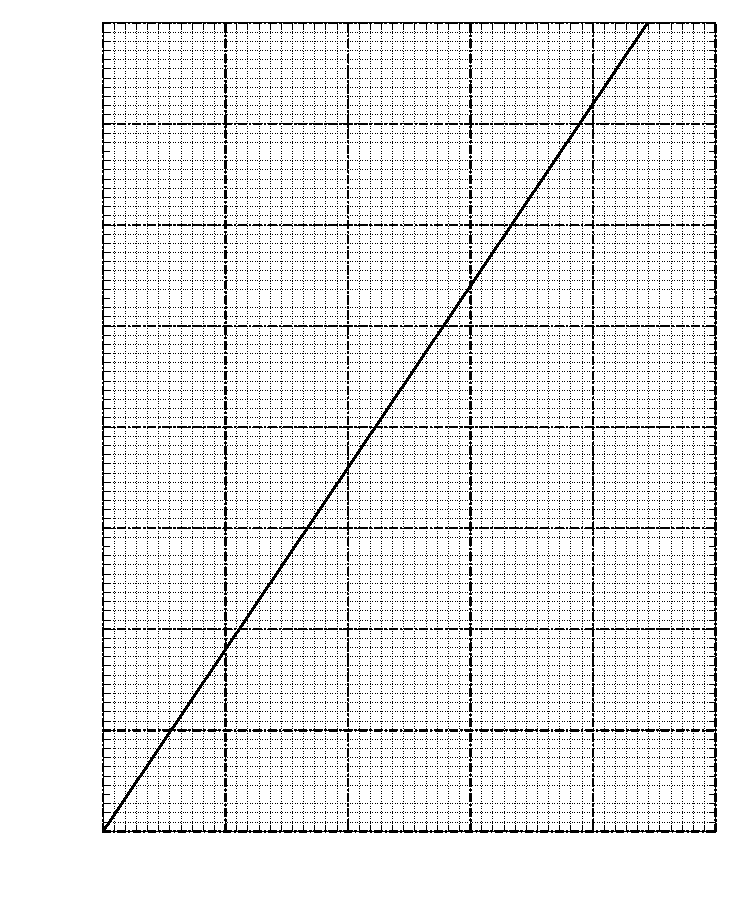
\includegraphics{../graphs/temp_conv}}%
    \gplfronttext
  \end{picture}%
\endgroup
\end{center}  % for gnuplot epslatex, latex or pslatex mode
}
\caption{Temperature Conversion Chart}
\label{Temp-comp-chart}
\end{figure}

        % Temperature Conversion Chart
% Weight Conversion Chart
\begin{figure}[t]
% \addcontentsline{toc}{section}{Figure \ref{Weight-comp-chart} Weight Conversion Chart}
\addcontentsline{toc}{section}{WEIGHT CONVERSION CHART}
\centering{
  \begin{perfhdr}WEIGHT CONVERSION CHART\\
  \end{perfhdr}
  \begin{center}
  % GNUPLOT: LaTeX picture with Postscript
\begingroup
  \makeatletter
  \providecommand\color[2][]{%
    \GenericError{(gnuplot) \space\space\space\@spaces}{%
      Package color not loaded in conjunction with
      terminal option `colourtext'%
    }{See the gnuplot documentation for explanation.%
    }{Either use 'blacktext' in gnuplot or load the package
      color.sty in LaTeX.}%
    \renewcommand\color[2][]{}%
  }%
  \providecommand\includegraphics[2][]{%
    \GenericError{(gnuplot) \space\space\space\@spaces}{%
      Package graphicx or graphics not loaded%
    }{See the gnuplot documentation for explanation.%
    }{The gnuplot epslatex terminal needs graphicx.sty or graphics.sty.}%
    \renewcommand\includegraphics[2][]{}%
  }%
  \providecommand\rotatebox[2]{#2}%
  \@ifundefined{ifGPcolor}{%
    \newif\ifGPcolor
    \GPcolorfalse
  }{}%
  \@ifundefined{ifGPblacktext}{%
    \newif\ifGPblacktext
    \GPblacktexttrue
  }{}%
  % define a \g@addto@macro without @ in the name:
  \let\gplgaddtomacro\g@addto@macro
  % define empty templates for all commands taking text:
  \gdef\gplbacktext{}%
  \gdef\gplfronttext{}%
  \makeatother
  \ifGPblacktext
    % no textcolor at all
    \def\colorrgb#1{}%
    \def\colorgray#1{}%
  \else
    % gray or color?
    \ifGPcolor
      \def\colorrgb#1{\color[rgb]{#1}}%
      \def\colorgray#1{\color[gray]{#1}}%
      \expandafter\def\csname LTw\endcsname{\color{white}}%
      \expandafter\def\csname LTb\endcsname{\color{black}}%
      \expandafter\def\csname LTa\endcsname{\color{black}}%
      \expandafter\def\csname LT0\endcsname{\color[rgb]{1,0,0}}%
      \expandafter\def\csname LT1\endcsname{\color[rgb]{0,1,0}}%
      \expandafter\def\csname LT2\endcsname{\color[rgb]{0,0,1}}%
      \expandafter\def\csname LT3\endcsname{\color[rgb]{1,0,1}}%
      \expandafter\def\csname LT4\endcsname{\color[rgb]{0,1,1}}%
      \expandafter\def\csname LT5\endcsname{\color[rgb]{1,1,0}}%
      \expandafter\def\csname LT6\endcsname{\color[rgb]{0,0,0}}%
      \expandafter\def\csname LT7\endcsname{\color[rgb]{1,0.3,0}}%
      \expandafter\def\csname LT8\endcsname{\color[rgb]{0.5,0.5,0.5}}%
    \else
      % gray
      \def\colorrgb#1{\color{black}}%
      \def\colorgray#1{\color[gray]{#1}}%
      \expandafter\def\csname LTw\endcsname{\color{white}}%
      \expandafter\def\csname LTb\endcsname{\color{black}}%
      \expandafter\def\csname LTa\endcsname{\color{black}}%
      \expandafter\def\csname LT0\endcsname{\color{black}}%
      \expandafter\def\csname LT1\endcsname{\color{black}}%
      \expandafter\def\csname LT2\endcsname{\color{black}}%
      \expandafter\def\csname LT3\endcsname{\color{black}}%
      \expandafter\def\csname LT4\endcsname{\color{black}}%
      \expandafter\def\csname LT5\endcsname{\color{black}}%
      \expandafter\def\csname LT6\endcsname{\color{black}}%
      \expandafter\def\csname LT7\endcsname{\color{black}}%
      \expandafter\def\csname LT8\endcsname{\color{black}}%
    \fi
  \fi
  \setlength{\unitlength}{0.0500bp}%
  \begin{picture}(7200.00,10080.00)%
    \gplgaddtomacro\gplbacktext{%
      \csname LTb\endcsname%
      \put(1210,704){\makebox(0,0)[r]{\strut{} 0}}%
      \csname LTb\endcsname%
      \put(1210,1615){\makebox(0,0)[r]{\strut{} 200}}%
      \csname LTb\endcsname%
      \put(1210,2526){\makebox(0,0)[r]{\strut{} 400}}%
      \csname LTb\endcsname%
      \put(1210,3437){\makebox(0,0)[r]{\strut{} 600}}%
      \csname LTb\endcsname%
      \put(1210,4348){\makebox(0,0)[r]{\strut{} 800}}%
      \csname LTb\endcsname%
      \put(1210,5259){\makebox(0,0)[r]{\strut{} 1000}}%
      \csname LTb\endcsname%
      \put(1210,6170){\makebox(0,0)[r]{\strut{} 1200}}%
      \csname LTb\endcsname%
      \put(1210,7081){\makebox(0,0)[r]{\strut{} 1400}}%
      \csname LTb\endcsname%
      \put(1210,7992){\makebox(0,0)[r]{\strut{} 1600}}%
      \csname LTb\endcsname%
      \put(1210,8903){\makebox(0,0)[r]{\strut{} 1800}}%
      \csname LTb\endcsname%
      \put(1210,9814){\makebox(0,0)[r]{\strut{} 2000}}%
      \csname LTb\endcsname%
      \put(1342,484){\makebox(0,0){\strut{} 0}}%
      \csname LTb\endcsname%
      \put(1956,484){\makebox(0,0){\strut{} 100}}%
      \csname LTb\endcsname%
      \put(2570,484){\makebox(0,0){\strut{} 200}}%
      \csname LTb\endcsname%
      \put(3184,484){\makebox(0,0){\strut{} 300}}%
      \csname LTb\endcsname%
      \put(3798,484){\makebox(0,0){\strut{} 400}}%
      \csname LTb\endcsname%
      \put(4413,484){\makebox(0,0){\strut{} 500}}%
      \csname LTb\endcsname%
      \put(5027,484){\makebox(0,0){\strut{} 600}}%
      \csname LTb\endcsname%
      \put(5641,484){\makebox(0,0){\strut{} 700}}%
      \csname LTb\endcsname%
      \put(6255,484){\makebox(0,0){\strut{} 800}}%
      \csname LTb\endcsname%
      \put(6869,484){\makebox(0,0){\strut{} 900}}%
      \put(308,5259){\rotatebox{-270}{\makebox(0,0){\strut{}Weight (lb)}}}%
      \put(4105,154){\makebox(0,0){\strut{}Mass (kg)}}%
    }%
    \gplgaddtomacro\gplfronttext{%
    }%
    \gplbacktext
    \put(0,0){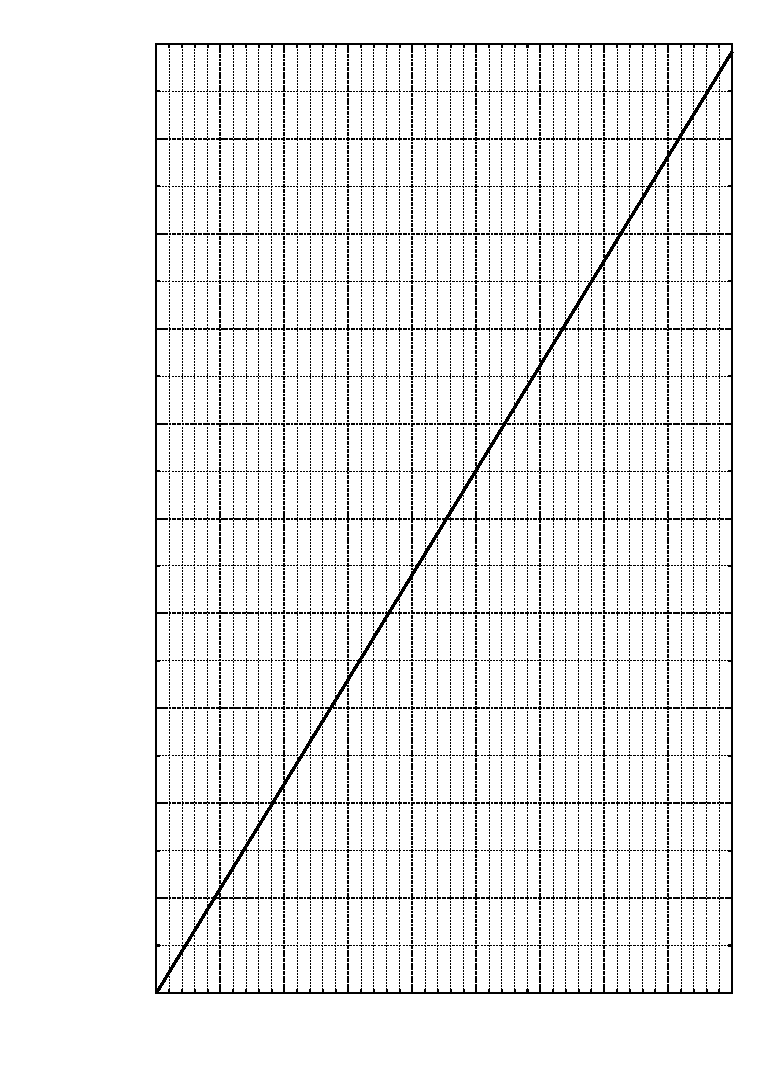
\includegraphics{../graphs/wt_conv}}%
    \gplfronttext
  \end{picture}%
\endgroup
\end{center}  % for gnuplot epslatex, latex or pslatex mode
}
\caption{Weight Conversion Chart}
\label{Weight-comp-chart}
\end{figure}

      % Weight Conversion Chart
% Volume Conversion Chart
\begin{figure}[t]
% \addcontentsline{toc}{section}{Figure \ref{Weight-comp-chart} Volume Conversion Chart}
\addcontentsline{toc}{section}{VOLUME CONVERSION CHART}
\centering{
  \begin{perfhdr}VOLUME CONVERSION CHART\\
  \end{perfhdr}
  \begin{center}
  % GNUPLOT: LaTeX picture with Postscript
\begingroup
  \makeatletter
  \providecommand\color[2][]{%
    \GenericError{(gnuplot) \space\space\space\@spaces}{%
      Package color not loaded in conjunction with
      terminal option `colourtext'%
    }{See the gnuplot documentation for explanation.%
    }{Either use 'blacktext' in gnuplot or load the package
      color.sty in LaTeX.}%
    \renewcommand\color[2][]{}%
  }%
  \providecommand\includegraphics[2][]{%
    \GenericError{(gnuplot) \space\space\space\@spaces}{%
      Package graphicx or graphics not loaded%
    }{See the gnuplot documentation for explanation.%
    }{The gnuplot epslatex terminal needs graphicx.sty or graphics.sty.}%
    \renewcommand\includegraphics[2][]{}%
  }%
  \providecommand\rotatebox[2]{#2}%
  \@ifundefined{ifGPcolor}{%
    \newif\ifGPcolor
    \GPcolorfalse
  }{}%
  \@ifundefined{ifGPblacktext}{%
    \newif\ifGPblacktext
    \GPblacktexttrue
  }{}%
  % define a \g@addto@macro without @ in the name:
  \let\gplgaddtomacro\g@addto@macro
  % define empty templates for all commands taking text:
  \gdef\gplbacktext{}%
  \gdef\gplfronttext{}%
  \makeatother
  \ifGPblacktext
    % no textcolor at all
    \def\colorrgb#1{}%
    \def\colorgray#1{}%
  \else
    % gray or color?
    \ifGPcolor
      \def\colorrgb#1{\color[rgb]{#1}}%
      \def\colorgray#1{\color[gray]{#1}}%
      \expandafter\def\csname LTw\endcsname{\color{white}}%
      \expandafter\def\csname LTb\endcsname{\color{black}}%
      \expandafter\def\csname LTa\endcsname{\color{black}}%
      \expandafter\def\csname LT0\endcsname{\color[rgb]{1,0,0}}%
      \expandafter\def\csname LT1\endcsname{\color[rgb]{0,1,0}}%
      \expandafter\def\csname LT2\endcsname{\color[rgb]{0,0,1}}%
      \expandafter\def\csname LT3\endcsname{\color[rgb]{1,0,1}}%
      \expandafter\def\csname LT4\endcsname{\color[rgb]{0,1,1}}%
      \expandafter\def\csname LT5\endcsname{\color[rgb]{1,1,0}}%
      \expandafter\def\csname LT6\endcsname{\color[rgb]{0,0,0}}%
      \expandafter\def\csname LT7\endcsname{\color[rgb]{1,0.3,0}}%
      \expandafter\def\csname LT8\endcsname{\color[rgb]{0.5,0.5,0.5}}%
    \else
      % gray
      \def\colorrgb#1{\color{black}}%
      \def\colorgray#1{\color[gray]{#1}}%
      \expandafter\def\csname LTw\endcsname{\color{white}}%
      \expandafter\def\csname LTb\endcsname{\color{black}}%
      \expandafter\def\csname LTa\endcsname{\color{black}}%
      \expandafter\def\csname LT0\endcsname{\color{black}}%
      \expandafter\def\csname LT1\endcsname{\color{black}}%
      \expandafter\def\csname LT2\endcsname{\color{black}}%
      \expandafter\def\csname LT3\endcsname{\color{black}}%
      \expandafter\def\csname LT4\endcsname{\color{black}}%
      \expandafter\def\csname LT5\endcsname{\color{black}}%
      \expandafter\def\csname LT6\endcsname{\color{black}}%
      \expandafter\def\csname LT7\endcsname{\color{black}}%
      \expandafter\def\csname LT8\endcsname{\color{black}}%
    \fi
  \fi
  \setlength{\unitlength}{0.0500bp}%
  \begin{picture}(7200.00,10080.00)%
    \gplgaddtomacro\gplbacktext{%
      \csname LTb\endcsname%
      \put(1078,704){\makebox(0,0)[r]{\strut{} 0}}%
      \csname LTb\endcsname%
      \put(1078,1615){\makebox(0,0)[r]{\strut{} 20}}%
      \csname LTb\endcsname%
      \put(1078,2526){\makebox(0,0)[r]{\strut{} 40}}%
      \csname LTb\endcsname%
      \put(1078,3437){\makebox(0,0)[r]{\strut{} 60}}%
      \csname LTb\endcsname%
      \put(1078,4348){\makebox(0,0)[r]{\strut{} 80}}%
      \csname LTb\endcsname%
      \put(1078,5259){\makebox(0,0)[r]{\strut{} 100}}%
      \csname LTb\endcsname%
      \put(1078,6170){\makebox(0,0)[r]{\strut{} 120}}%
      \csname LTb\endcsname%
      \put(1078,7081){\makebox(0,0)[r]{\strut{} 140}}%
      \csname LTb\endcsname%
      \put(1078,7992){\makebox(0,0)[r]{\strut{} 160}}%
      \csname LTb\endcsname%
      \put(1078,8903){\makebox(0,0)[r]{\strut{} 180}}%
      \csname LTb\endcsname%
      \put(1078,9814){\makebox(0,0)[r]{\strut{} 200}}%
      \csname LTb\endcsname%
      \put(1210,484){\makebox(0,0){\strut{} 0}}%
      \csname LTb\endcsname%
      \put(2342,484){\makebox(0,0){\strut{} 10}}%
      \csname LTb\endcsname%
      \put(3474,484){\makebox(0,0){\strut{} 20}}%
      \csname LTb\endcsname%
      \put(4605,484){\makebox(0,0){\strut{} 30}}%
      \csname LTb\endcsname%
      \put(5737,484){\makebox(0,0){\strut{} 40}}%
      \csname LTb\endcsname%
      \put(6869,484){\makebox(0,0){\strut{} 50}}%
      \put(308,5259){\rotatebox{-270}{\makebox(0,0){\strut{}Volume (l)}}}%
      \put(4039,154){\makebox(0,0){\strut{}Volume (USG)}}%
    }%
    \gplgaddtomacro\gplfronttext{%
    }%
    \gplbacktext
    \put(0,0){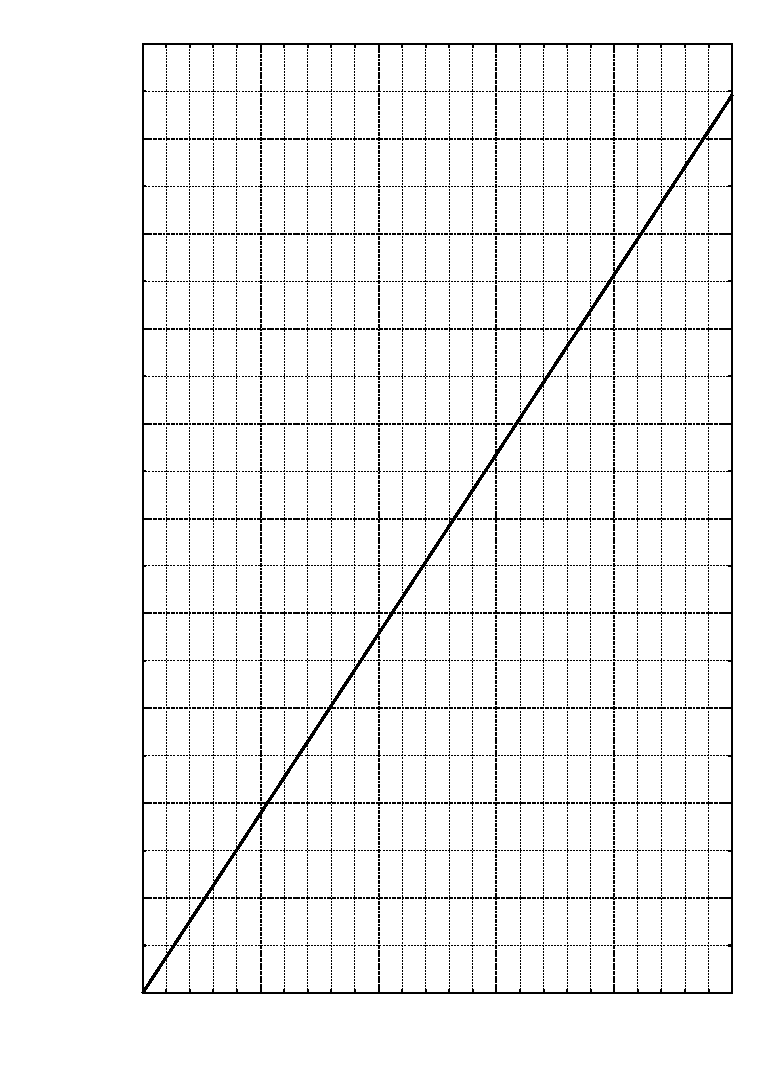
\includegraphics{../graphs/vol_conv}}%
    \gplfronttext
  \end{picture}%
\endgroup
\end{center}  % for gnuplot epslatex, latex or pslatex mode
}
\caption{Volume Conversion Chart}
\label{Volume-comp-chart}
\end{figure}

         % Volume Conversion Chart
% Static Source Position Error, Airspeed Chart
%% try boxedminipage.sty to get box around figure, to help separate two figures if there are more than one per page
\begin{figure}[t]
% \addcontentsline{toc}{section}{Figure \ref{SSEC-spd-error} Position Error --- Airspeed --- Flaps Retracted}
\addcontentsline{toc}{section}{POSITION ERROR --- AIRSPEED --- FLAPS RETRACTED}
\centering{
  \begin{perfhdr}POSITION ERROR --- AIRSPEED\\
  FLAPS RETRACTED\\
  \end{perfhdr}

  \centering{\begin{minipage}{5in}\begin{tabbing}
  EFIS Make - Model:aaaaa\= \kill
  Weight:\>1400 lb\\
  Flaps:\>Retracted\\
  Date of flight tests:\>14 \& 19 Nov 2008
  \end{tabbing}\end{minipage}}
  \begin{center}
  % GNUPLOT: LaTeX picture with Postscript
\begingroup
  \makeatletter
  \providecommand\color[2][]{%
    \GenericError{(gnuplot) \space\space\space\@spaces}{%
      Package color not loaded in conjunction with
      terminal option `colourtext'%
    }{See the gnuplot documentation for explanation.%
    }{Either use 'blacktext' in gnuplot or load the package
      color.sty in LaTeX.}%
    \renewcommand\color[2][]{}%
  }%
  \providecommand\includegraphics[2][]{%
    \GenericError{(gnuplot) \space\space\space\@spaces}{%
      Package graphicx or graphics not loaded%
    }{See the gnuplot documentation for explanation.%
    }{The gnuplot epslatex terminal needs graphicx.sty or graphics.sty.}%
    \renewcommand\includegraphics[2][]{}%
  }%
  \providecommand\rotatebox[2]{#2}%
  \@ifundefined{ifGPcolor}{%
    \newif\ifGPcolor
    \GPcolorfalse
  }{}%
  \@ifundefined{ifGPblacktext}{%
    \newif\ifGPblacktext
    \GPblacktexttrue
  }{}%
  % define a \g@addto@macro without @ in the name:
  \let\gplgaddtomacro\g@addto@macro
  % define empty templates for all commands taking text:
  \gdef\gplbacktext{}%
  \gdef\gplfronttext{}%
  \makeatother
  \ifGPblacktext
    % no textcolor at all
    \def\colorrgb#1{}%
    \def\colorgray#1{}%
  \else
    % gray or color?
    \ifGPcolor
      \def\colorrgb#1{\color[rgb]{#1}}%
      \def\colorgray#1{\color[gray]{#1}}%
      \expandafter\def\csname LTw\endcsname{\color{white}}%
      \expandafter\def\csname LTb\endcsname{\color{black}}%
      \expandafter\def\csname LTa\endcsname{\color{black}}%
      \expandafter\def\csname LT0\endcsname{\color[rgb]{1,0,0}}%
      \expandafter\def\csname LT1\endcsname{\color[rgb]{0,1,0}}%
      \expandafter\def\csname LT2\endcsname{\color[rgb]{0,0,1}}%
      \expandafter\def\csname LT3\endcsname{\color[rgb]{1,0,1}}%
      \expandafter\def\csname LT4\endcsname{\color[rgb]{0,1,1}}%
      \expandafter\def\csname LT5\endcsname{\color[rgb]{1,1,0}}%
      \expandafter\def\csname LT6\endcsname{\color[rgb]{0,0,0}}%
      \expandafter\def\csname LT7\endcsname{\color[rgb]{1,0.3,0}}%
      \expandafter\def\csname LT8\endcsname{\color[rgb]{0.5,0.5,0.5}}%
    \else
      % gray
      \def\colorrgb#1{\color{black}}%
      \def\colorgray#1{\color[gray]{#1}}%
      \expandafter\def\csname LTw\endcsname{\color{white}}%
      \expandafter\def\csname LTb\endcsname{\color{black}}%
      \expandafter\def\csname LTa\endcsname{\color{black}}%
      \expandafter\def\csname LT0\endcsname{\color{black}}%
      \expandafter\def\csname LT1\endcsname{\color{black}}%
      \expandafter\def\csname LT2\endcsname{\color{black}}%
      \expandafter\def\csname LT3\endcsname{\color{black}}%
      \expandafter\def\csname LT4\endcsname{\color{black}}%
      \expandafter\def\csname LT5\endcsname{\color{black}}%
      \expandafter\def\csname LT6\endcsname{\color{black}}%
      \expandafter\def\csname LT7\endcsname{\color{black}}%
      \expandafter\def\csname LT8\endcsname{\color{black}}%
    \fi
  \fi
  \setlength{\unitlength}{0.0500bp}%
  \begin{picture}(7200.00,5040.00)%
    \gplgaddtomacro\gplbacktext{%
      \csname LTb\endcsname%
      \put(1078,704){\makebox(0,0)[r]{\strut{}-5}}%
      \csname LTb\endcsname%
      \put(1078,1038){\makebox(0,0)[r]{\strut{}-4.5}}%
      \csname LTb\endcsname%
      \put(1078,1372){\makebox(0,0)[r]{\strut{}-4}}%
      \csname LTb\endcsname%
      \put(1078,1706){\makebox(0,0)[r]{\strut{}-3.5}}%
      \csname LTb\endcsname%
      \put(1078,2040){\makebox(0,0)[r]{\strut{}-3}}%
      \csname LTb\endcsname%
      \put(1078,2374){\makebox(0,0)[r]{\strut{}-2.5}}%
      \csname LTb\endcsname%
      \put(1078,2709){\makebox(0,0)[r]{\strut{}-2}}%
      \csname LTb\endcsname%
      \put(1078,3043){\makebox(0,0)[r]{\strut{}-1.5}}%
      \csname LTb\endcsname%
      \put(1078,3377){\makebox(0,0)[r]{\strut{}-1}}%
      \csname LTb\endcsname%
      \put(1078,3711){\makebox(0,0)[r]{\strut{}-0.5}}%
      \csname LTb\endcsname%
      \put(1078,4045){\makebox(0,0)[r]{\strut{} 0}}%
      \csname LTb\endcsname%
      \put(1078,4379){\makebox(0,0)[r]{\strut{} 0.5}}%
      \csname LTb\endcsname%
      \put(1210,484){\makebox(0,0){\strut{} 50}}%
      \csname LTb\endcsname%
      \put(2625,484){\makebox(0,0){\strut{} 100}}%
      \csname LTb\endcsname%
      \put(4040,484){\makebox(0,0){\strut{} 150}}%
      \csname LTb\endcsname%
      \put(5454,484){\makebox(0,0){\strut{} 200}}%
      \csname LTb\endcsname%
      \put(6869,484){\makebox(0,0){\strut{} 250}}%
      \put(308,2541){\rotatebox{-270}{\makebox(0,0){\strut{}Position Error in Airspeed (kt)}}}%
      \put(4039,154){\makebox(0,0){\strut{}IAS - instrument corrected (kt)}}%
      \put(4039,4709){\makebox(0,0){\strut{}Static Source Position Error - Airspeed - Flaps Retracted}}%
    }%
    \gplgaddtomacro\gplfronttext{%
      \put(3332,2207){\makebox(0,0){\strut{}CAS = IAS + Error}}%
      \put(3332,1873){\makebox(0,0){\strut{}ASI Instrument Error Assumed to be Zero}}%
    }%
    \gplbacktext
    \put(0,0){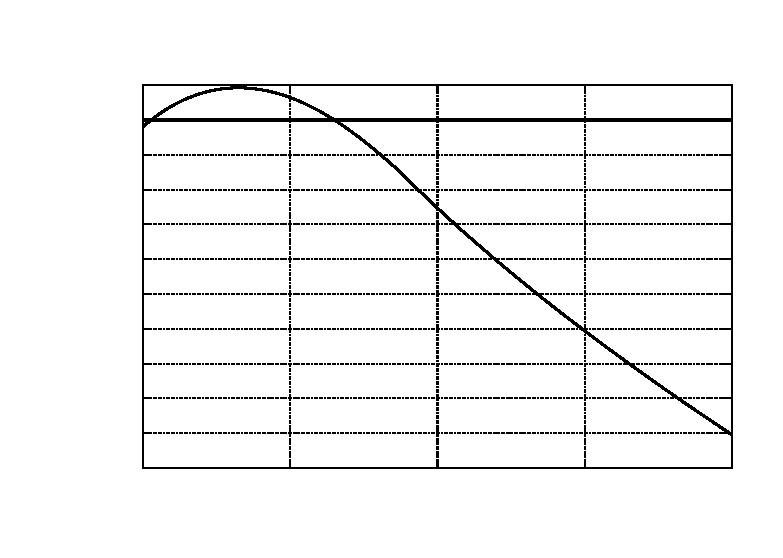
\includegraphics{../graphs/ias_error_no_inst_corr_flaps_up}}%
    \gplfronttext
  \end{picture}%
\endgroup
\end{center}  % for gnuplot epslatex, latex or pslatex mode
}
\caption{Position Error --- Airspeed --- Flaps Retracted}
\label{SSEC-spd-error}
\end{figure}

               % Static Source Position Error, Airspeed Chart
% Static Source Position Error, Altitude Chart
%% try boxedminipage.sty to get box around figure, to help separate two figures if there are more than one per page
\begin{figure}[t]
% \addcontentsline{toc}{section}{Figure \ref{SSEC-alt-error} Position Error --- Altitude --- Flaps Retracted}
\addcontentsline{toc}{section}{POSITION ERROR --- ALTITUDE --- FLAPS RETRACTED}
\centering{
  \begin{perfhdr}POSITION ERROR --- ALTITUDE\\
  FLAPS RETRACTED\\
  \end{perfhdr}

  \centering{\begin{minipage}{5in}\begin{tabbing}
  EFIS Make - Model:aaaaa\= \kill
  Weight:\>1600 lb\\
  Flaps:\>Retracted\\
  Date of flight tests:\>14 \& 19 Nov 2008
  \end{tabbing}\end{minipage}}
  \begin{center}
  % GNUPLOT: LaTeX picture with Postscript
\begingroup
  \makeatletter
  \providecommand\color[2][]{%
    \GenericError{(gnuplot) \space\space\space\@spaces}{%
      Package color not loaded in conjunction with
      terminal option `colourtext'%
    }{See the gnuplot documentation for explanation.%
    }{Either use 'blacktext' in gnuplot or load the package
      color.sty in LaTeX.}%
    \renewcommand\color[2][]{}%
  }%
  \providecommand\includegraphics[2][]{%
    \GenericError{(gnuplot) \space\space\space\@spaces}{%
      Package graphicx or graphics not loaded%
    }{See the gnuplot documentation for explanation.%
    }{The gnuplot epslatex terminal needs graphicx.sty or graphics.sty.}%
    \renewcommand\includegraphics[2][]{}%
  }%
  \providecommand\rotatebox[2]{#2}%
  \@ifundefined{ifGPcolor}{%
    \newif\ifGPcolor
    \GPcolorfalse
  }{}%
  \@ifundefined{ifGPblacktext}{%
    \newif\ifGPblacktext
    \GPblacktexttrue
  }{}%
  % define a \g@addto@macro without @ in the name:
  \let\gplgaddtomacro\g@addto@macro
  % define empty templates for all commands taking text:
  \gdef\gplbacktext{}%
  \gdef\gplfronttext{}%
  \makeatother
  \ifGPblacktext
    % no textcolor at all
    \def\colorrgb#1{}%
    \def\colorgray#1{}%
  \else
    % gray or color?
    \ifGPcolor
      \def\colorrgb#1{\color[rgb]{#1}}%
      \def\colorgray#1{\color[gray]{#1}}%
      \expandafter\def\csname LTw\endcsname{\color{white}}%
      \expandafter\def\csname LTb\endcsname{\color{black}}%
      \expandafter\def\csname LTa\endcsname{\color{black}}%
      \expandafter\def\csname LT0\endcsname{\color[rgb]{1,0,0}}%
      \expandafter\def\csname LT1\endcsname{\color[rgb]{0,1,0}}%
      \expandafter\def\csname LT2\endcsname{\color[rgb]{0,0,1}}%
      \expandafter\def\csname LT3\endcsname{\color[rgb]{1,0,1}}%
      \expandafter\def\csname LT4\endcsname{\color[rgb]{0,1,1}}%
      \expandafter\def\csname LT5\endcsname{\color[rgb]{1,1,0}}%
      \expandafter\def\csname LT6\endcsname{\color[rgb]{0,0,0}}%
      \expandafter\def\csname LT7\endcsname{\color[rgb]{1,0.3,0}}%
      \expandafter\def\csname LT8\endcsname{\color[rgb]{0.5,0.5,0.5}}%
    \else
      % gray
      \def\colorrgb#1{\color{black}}%
      \def\colorgray#1{\color[gray]{#1}}%
      \expandafter\def\csname LTw\endcsname{\color{white}}%
      \expandafter\def\csname LTb\endcsname{\color{black}}%
      \expandafter\def\csname LTa\endcsname{\color{black}}%
      \expandafter\def\csname LT0\endcsname{\color{black}}%
      \expandafter\def\csname LT1\endcsname{\color{black}}%
      \expandafter\def\csname LT2\endcsname{\color{black}}%
      \expandafter\def\csname LT3\endcsname{\color{black}}%
      \expandafter\def\csname LT4\endcsname{\color{black}}%
      \expandafter\def\csname LT5\endcsname{\color{black}}%
      \expandafter\def\csname LT6\endcsname{\color{black}}%
      \expandafter\def\csname LT7\endcsname{\color{black}}%
      \expandafter\def\csname LT8\endcsname{\color{black}}%
    \fi
  \fi
  \setlength{\unitlength}{0.0500bp}%
  \begin{picture}(7200.00,5040.00)%
    \gplgaddtomacro\gplbacktext{%
      \csname LTb\endcsname%
      \put(946,704){\makebox(0,0)[r]{\strut{}-90}}%
      \csname LTb\endcsname%
      \put(946,1072){\makebox(0,0)[r]{\strut{}-80}}%
      \csname LTb\endcsname%
      \put(946,1439){\makebox(0,0)[r]{\strut{}-70}}%
      \csname LTb\endcsname%
      \put(946,1807){\makebox(0,0)[r]{\strut{}-60}}%
      \csname LTb\endcsname%
      \put(946,2174){\makebox(0,0)[r]{\strut{}-50}}%
      \csname LTb\endcsname%
      \put(946,2542){\makebox(0,0)[r]{\strut{}-40}}%
      \csname LTb\endcsname%
      \put(946,2909){\makebox(0,0)[r]{\strut{}-30}}%
      \csname LTb\endcsname%
      \put(946,3277){\makebox(0,0)[r]{\strut{}-20}}%
      \csname LTb\endcsname%
      \put(946,3644){\makebox(0,0)[r]{\strut{}-10}}%
      \csname LTb\endcsname%
      \put(946,4012){\makebox(0,0)[r]{\strut{} 0}}%
      \csname LTb\endcsname%
      \put(946,4379){\makebox(0,0)[r]{\strut{} 10}}%
      \csname LTb\endcsname%
      \put(1464,484){\makebox(0,0){\strut{} 60}}%
      \csname LTb\endcsname%
      \put(2236,484){\makebox(0,0){\strut{} 80}}%
      \csname LTb\endcsname%
      \put(3008,484){\makebox(0,0){\strut{} 100}}%
      \csname LTb\endcsname%
      \put(3780,484){\makebox(0,0){\strut{} 120}}%
      \csname LTb\endcsname%
      \put(4553,484){\makebox(0,0){\strut{} 140}}%
      \csname LTb\endcsname%
      \put(5325,484){\makebox(0,0){\strut{} 160}}%
      \csname LTb\endcsname%
      \put(6097,484){\makebox(0,0){\strut{} 180}}%
      \csname LTb\endcsname%
      \put(6869,484){\makebox(0,0){\strut{} 200}}%
      \put(308,2541){\rotatebox{-270}{\makebox(0,0){\strut{}Position Error in Altitude (ft)}}}%
      \put(3973,154){\makebox(0,0){\strut{}IAS - instrument corrected (kt)}}%
      \put(3973,4709){\makebox(0,0){\strut{}Static Source Position Error - Altitude - Flaps Retracted}}%
    }%
    \gplgaddtomacro\gplfronttext{%
      \put(3974,1623){\makebox(0,0){\strut{}Baro Altitude = Altimeter Reading + Error}}%
      \put(3974,1255){\makebox(0,0){\strut{}ASI and Altimeter Instrument Errors Assumed to be Zero}}%
      \put(6097,3111){\rotatebox{-36}{\makebox(0,0)[l]{\strut{}Sea Level}}}%
      \put(6097,2762){\rotatebox{-44}{\makebox(0,0)[l]{\strut{}10,000 ft}}}%
      \put(6097,2284){\rotatebox{-53}{\makebox(0,0)[l]{\strut{}20,000 ft}}}%
    }%
    \gplbacktext
    \put(0,0){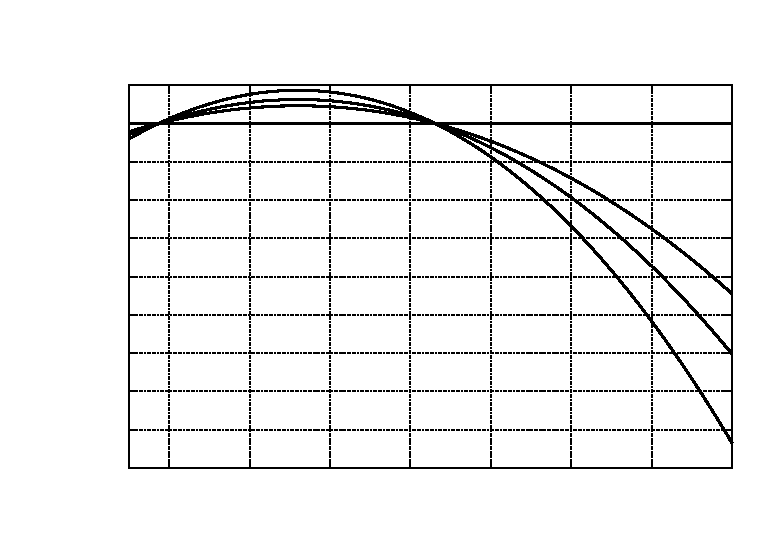
\includegraphics{../graphs/alt_error_flaps_up}}%
    \gplfronttext
  \end{picture}%
\endgroup
\end{center}  % for gnuplot epslatex, latex or pslatex mode
}
\caption{Position Error --- Altitude --- Flaps Retracted}
\label{SSEC-alt-error}
\end{figure}

               % Static Source Position Error, Altitude Chart
% ASI Instrument Error Chart
\begin{figure}[t]
% \addcontentsline{toc}{section}{Figure \ref{fg-asi-error} Airspeed Indicator Instrument Error}
\addcontentsline{toc}{section}{AIRSPEED INDICATOR INSTRUMENT ERROR}
%\addcontentsline{toc}{section}{Figure \ref{fg-asi-error} AIRSPEED INDICATOR INSTRUMENT ERROR}
\centering{
  \begin{perfhdr}AIRSPEED INDICATOR\\
  INSTRUMENT ERROR\\
  \end{perfhdr}
  % details of ASI
  \centering{\begin{minipage}{5in}\begin{tabbing}
  ASI Make - Model:aaaaa\= \kill
  ASI Make \& Model:\>UMA 16-311-241\\
  Serial \#:\>B0171\\
  Date of ground test:\>27 Apr 2004
  \end{tabbing}\end{minipage}}
  \begin{center}
  % GNUPLOT: LaTeX picture with Postscript
\begingroup
  \makeatletter
  \providecommand\color[2][]{%
    \GenericError{(gnuplot) \space\space\space\@spaces}{%
      Package color not loaded in conjunction with
      terminal option `colourtext'%
    }{See the gnuplot documentation for explanation.%
    }{Either use 'blacktext' in gnuplot or load the package
      color.sty in LaTeX.}%
    \renewcommand\color[2][]{}%
  }%
  \providecommand\includegraphics[2][]{%
    \GenericError{(gnuplot) \space\space\space\@spaces}{%
      Package graphicx or graphics not loaded%
    }{See the gnuplot documentation for explanation.%
    }{The gnuplot epslatex terminal needs graphicx.sty or graphics.sty.}%
    \renewcommand\includegraphics[2][]{}%
  }%
  \providecommand\rotatebox[2]{#2}%
  \@ifundefined{ifGPcolor}{%
    \newif\ifGPcolor
    \GPcolorfalse
  }{}%
  \@ifundefined{ifGPblacktext}{%
    \newif\ifGPblacktext
    \GPblacktexttrue
  }{}%
  % define a \g@addto@macro without @ in the name:
  \let\gplgaddtomacro\g@addto@macro
  % define empty templates for all commands taking text:
  \gdef\gplbacktext{}%
  \gdef\gplfronttext{}%
  \makeatother
  \ifGPblacktext
    % no textcolor at all
    \def\colorrgb#1{}%
    \def\colorgray#1{}%
  \else
    % gray or color?
    \ifGPcolor
      \def\colorrgb#1{\color[rgb]{#1}}%
      \def\colorgray#1{\color[gray]{#1}}%
      \expandafter\def\csname LTw\endcsname{\color{white}}%
      \expandafter\def\csname LTb\endcsname{\color{black}}%
      \expandafter\def\csname LTa\endcsname{\color{black}}%
      \expandafter\def\csname LT0\endcsname{\color[rgb]{1,0,0}}%
      \expandafter\def\csname LT1\endcsname{\color[rgb]{0,1,0}}%
      \expandafter\def\csname LT2\endcsname{\color[rgb]{0,0,1}}%
      \expandafter\def\csname LT3\endcsname{\color[rgb]{1,0,1}}%
      \expandafter\def\csname LT4\endcsname{\color[rgb]{0,1,1}}%
      \expandafter\def\csname LT5\endcsname{\color[rgb]{1,1,0}}%
      \expandafter\def\csname LT6\endcsname{\color[rgb]{0,0,0}}%
      \expandafter\def\csname LT7\endcsname{\color[rgb]{1,0.3,0}}%
      \expandafter\def\csname LT8\endcsname{\color[rgb]{0.5,0.5,0.5}}%
    \else
      % gray
      \def\colorrgb#1{\color{black}}%
      \def\colorgray#1{\color[gray]{#1}}%
      \expandafter\def\csname LTw\endcsname{\color{white}}%
      \expandafter\def\csname LTb\endcsname{\color{black}}%
      \expandafter\def\csname LTa\endcsname{\color{black}}%
      \expandafter\def\csname LT0\endcsname{\color{black}}%
      \expandafter\def\csname LT1\endcsname{\color{black}}%
      \expandafter\def\csname LT2\endcsname{\color{black}}%
      \expandafter\def\csname LT3\endcsname{\color{black}}%
      \expandafter\def\csname LT4\endcsname{\color{black}}%
      \expandafter\def\csname LT5\endcsname{\color{black}}%
      \expandafter\def\csname LT6\endcsname{\color{black}}%
      \expandafter\def\csname LT7\endcsname{\color{black}}%
      \expandafter\def\csname LT8\endcsname{\color{black}}%
    \fi
  \fi
  \setlength{\unitlength}{0.0500bp}%
  \begin{picture}(7200.00,5040.00)%
    \gplgaddtomacro\gplbacktext{%
      \csname LTb\endcsname%
      \put(814,704){\makebox(0,0)[r]{\strut{}-3}}%
      \csname LTb\endcsname%
      \put(814,1286){\makebox(0,0)[r]{\strut{}-2}}%
      \csname LTb\endcsname%
      \put(814,1867){\makebox(0,0)[r]{\strut{}-1}}%
      \csname LTb\endcsname%
      \put(814,2449){\makebox(0,0)[r]{\strut{} 0}}%
      \csname LTb\endcsname%
      \put(814,3030){\makebox(0,0)[r]{\strut{} 1}}%
      \csname LTb\endcsname%
      \put(814,3612){\makebox(0,0)[r]{\strut{} 2}}%
      \csname LTb\endcsname%
      \put(814,4193){\makebox(0,0)[r]{\strut{} 3}}%
      \csname LTb\endcsname%
      \put(814,4775){\makebox(0,0)[r]{\strut{} 4}}%
      \csname LTb\endcsname%
      \put(946,484){\makebox(0,0){\strut{} 0}}%
      \csname LTb\endcsname%
      \put(2131,484){\makebox(0,0){\strut{} 50}}%
      \csname LTb\endcsname%
      \put(3315,484){\makebox(0,0){\strut{} 100}}%
      \csname LTb\endcsname%
      \put(4500,484){\makebox(0,0){\strut{} 150}}%
      \csname LTb\endcsname%
      \put(5684,484){\makebox(0,0){\strut{} 200}}%
      \csname LTb\endcsname%
      \put(6869,484){\makebox(0,0){\strut{} 250}}%
      \put(308,2739){\rotatebox{-270}{\makebox(0,0){\strut{}ASI Instrument Error (kt)}}}%
      \put(3907,154){\makebox(0,0){\strut{}Airspeed Indicator Reading (kt)}}%
    }%
    \gplgaddtomacro\gplfronttext{%
      \put(3789,3903){\makebox(0,0){\strut{}ASI Reading = IAS + Error}}%
    }%
    \gplbacktext
    \put(0,0){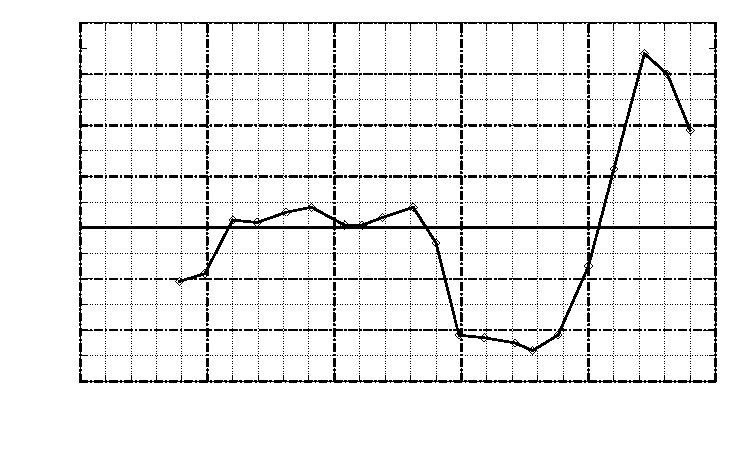
\includegraphics{../graphs/asi_error}}%
    \gplfronttext
  \end{picture}%
\endgroup

  \end{center}  % for gnuplot epslatex, latex or pslatex mode
}
\caption{Airspeed Indicator Instrument Error}
\label{fg-asi-error}
\end{figure}
%\lyxline{\normalsize}
%%%\vspace{0.1in}


         % ASI Instrument Error Chart
% EFIS Instrument Error Chart
%% try boxedminipage.sty to get box around figure, to help separate two figures if there are more than one per page
\begin{figure}[t]
% \addcontentsline{toc}{section}{Figure \ref{EFIS-asi-error} EFIS Airspeed Instrument Error}
\addcontentsline{toc}{section}{EFIS AIRSPEED INSTRUMENT ERROR}
\centering{
  \begin{perfhdr}EFIS AIRSPEED\\
  INSTRUMENT ERROR\\
  \end{perfhdr}
  % details of EFIS
  \centering{\begin{minipage}{5in}\begin{tabbing}
  EFIS Make - Model:aaaaa\= \kill
  EFIS Make \& Model:\>Dynon Development D-10A\\
  Part \#:\>100321- Rev 0\\
  Serial \#:\>004439\\
  Date of ground test:\>27 Apr 2004
  \end{tabbing}\end{minipage}}
  \begin{center}
  % GNUPLOT: LaTeX picture with Postscript
\begingroup
  \makeatletter
  \providecommand\color[2][]{%
    \GenericError{(gnuplot) \space\space\space\@spaces}{%
      Package color not loaded in conjunction with
      terminal option `colourtext'%
    }{See the gnuplot documentation for explanation.%
    }{Either use 'blacktext' in gnuplot or load the package
      color.sty in LaTeX.}%
    \renewcommand\color[2][]{}%
  }%
  \providecommand\includegraphics[2][]{%
    \GenericError{(gnuplot) \space\space\space\@spaces}{%
      Package graphicx or graphics not loaded%
    }{See the gnuplot documentation for explanation.%
    }{The gnuplot epslatex terminal needs graphicx.sty or graphics.sty.}%
    \renewcommand\includegraphics[2][]{}%
  }%
  \providecommand\rotatebox[2]{#2}%
  \@ifundefined{ifGPcolor}{%
    \newif\ifGPcolor
    \GPcolorfalse
  }{}%
  \@ifundefined{ifGPblacktext}{%
    \newif\ifGPblacktext
    \GPblacktexttrue
  }{}%
  % define a \g@addto@macro without @ in the name:
  \let\gplgaddtomacro\g@addto@macro
  % define empty templates for all commands taking text:
  \gdef\gplbacktext{}%
  \gdef\gplfronttext{}%
  \makeatother
  \ifGPblacktext
    % no textcolor at all
    \def\colorrgb#1{}%
    \def\colorgray#1{}%
  \else
    % gray or color?
    \ifGPcolor
      \def\colorrgb#1{\color[rgb]{#1}}%
      \def\colorgray#1{\color[gray]{#1}}%
      \expandafter\def\csname LTw\endcsname{\color{white}}%
      \expandafter\def\csname LTb\endcsname{\color{black}}%
      \expandafter\def\csname LTa\endcsname{\color{black}}%
      \expandafter\def\csname LT0\endcsname{\color[rgb]{1,0,0}}%
      \expandafter\def\csname LT1\endcsname{\color[rgb]{0,1,0}}%
      \expandafter\def\csname LT2\endcsname{\color[rgb]{0,0,1}}%
      \expandafter\def\csname LT3\endcsname{\color[rgb]{1,0,1}}%
      \expandafter\def\csname LT4\endcsname{\color[rgb]{0,1,1}}%
      \expandafter\def\csname LT5\endcsname{\color[rgb]{1,1,0}}%
      \expandafter\def\csname LT6\endcsname{\color[rgb]{0,0,0}}%
      \expandafter\def\csname LT7\endcsname{\color[rgb]{1,0.3,0}}%
      \expandafter\def\csname LT8\endcsname{\color[rgb]{0.5,0.5,0.5}}%
    \else
      % gray
      \def\colorrgb#1{\color{black}}%
      \def\colorgray#1{\color[gray]{#1}}%
      \expandafter\def\csname LTw\endcsname{\color{white}}%
      \expandafter\def\csname LTb\endcsname{\color{black}}%
      \expandafter\def\csname LTa\endcsname{\color{black}}%
      \expandafter\def\csname LT0\endcsname{\color{black}}%
      \expandafter\def\csname LT1\endcsname{\color{black}}%
      \expandafter\def\csname LT2\endcsname{\color{black}}%
      \expandafter\def\csname LT3\endcsname{\color{black}}%
      \expandafter\def\csname LT4\endcsname{\color{black}}%
      \expandafter\def\csname LT5\endcsname{\color{black}}%
      \expandafter\def\csname LT6\endcsname{\color{black}}%
      \expandafter\def\csname LT7\endcsname{\color{black}}%
      \expandafter\def\csname LT8\endcsname{\color{black}}%
    \fi
  \fi
  \setlength{\unitlength}{0.0500bp}%
  \begin{picture}(7200.00,5040.00)%
    \gplgaddtomacro\gplbacktext{%
      \csname LTb\endcsname%
      \put(814,704){\makebox(0,0)[r]{\strut{}-3}}%
      \csname LTb\endcsname%
      \put(814,1722){\makebox(0,0)[r]{\strut{}-2}}%
      \csname LTb\endcsname%
      \put(814,2740){\makebox(0,0)[r]{\strut{}-1}}%
      \csname LTb\endcsname%
      \put(814,3757){\makebox(0,0)[r]{\strut{} 0}}%
      \csname LTb\endcsname%
      \put(814,4775){\makebox(0,0)[r]{\strut{} 1}}%
      \csname LTb\endcsname%
      \put(946,484){\makebox(0,0){\strut{} 0}}%
      \csname LTb\endcsname%
      \put(2131,484){\makebox(0,0){\strut{} 50}}%
      \csname LTb\endcsname%
      \put(3315,484){\makebox(0,0){\strut{} 100}}%
      \csname LTb\endcsname%
      \put(4500,484){\makebox(0,0){\strut{} 150}}%
      \csname LTb\endcsname%
      \put(5684,484){\makebox(0,0){\strut{} 200}}%
      \csname LTb\endcsname%
      \put(6869,484){\makebox(0,0){\strut{} 250}}%
      \put(308,2739){\rotatebox{-270}{\makebox(0,0){\strut{}EFIS ASI Instrument Error (kt)}}}%
      \put(3907,154){\makebox(0,0){\strut{}EFIS Airspeed Reading (kt)}}%
    }%
    \gplgaddtomacro\gplfronttext{%
      \put(3789,1213){\makebox(0,0){\strut{}EFIS Airspeed Reading = IAS + Error}}%
    }%
    \gplbacktext
    \put(0,0){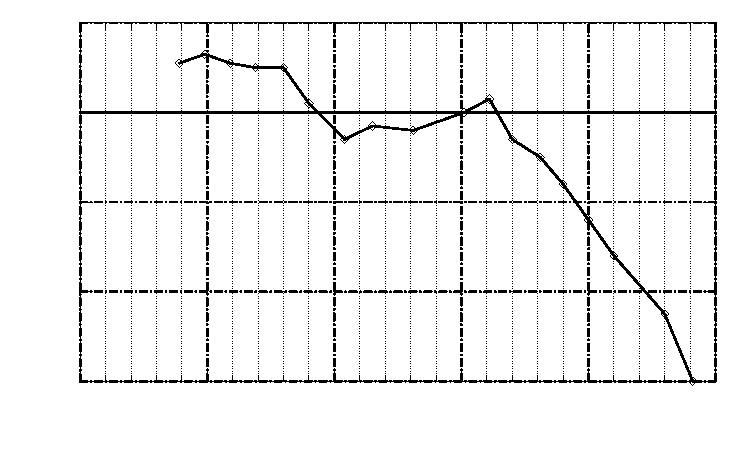
\includegraphics{../graphs/efis_error}}%
    \gplfronttext
  \end{picture}%
\endgroup
\end{center}  % for gnuplot epslatex, latex or pslatex mode
}
\caption{EFIS Airspeed Instrument Error}
\label{EFIS-asi-error}
\end{figure}


    % EFIS Instrument Error Chart
% EFIS Airspeed Error Chart --- Static Source Position Error + EFIS ASI instrument error
%% try boxedminipage.sty to get box around figure, to help separate two figures if there are more than one per page
\begin{figure}[t]
% \addcontentsline{toc}{section}{Figure \ref{EFIS-spd-error} EFIS Airspeed Error --- Airspeed --- Flaps Retracted}
\addcontentsline{toc}{section}{EFIS AIRSPEED ERROR --- AIRSPEED --- FLAPS RETRACTED}
\centering{
  \begin{perfhdr}EFIS AIRSPEED ERROR\\
  FLAPS RETRACTED\\
  \end{perfhdr}

  \centering{\begin{minipage}{5in}\begin{tabbing}
  EFIS Make --- Model:aaaaa\= \kill
  EFIS Make \& Model:\>Dynon Development D-10A\\
  Part \#:\>100321- Rev 0\\
  Serial \#:\>004439\\
  Date of ground test:\>27 Apr 2004\\
  \\
  Weight:\>1400 lb\\
  Flaps:\>Retracted\\
  Date of flight tests:\>14 \& 19 Nov 2008
  \end{tabbing}\end{minipage}}
  \begin{center}
  % GNUPLOT: LaTeX picture with Postscript
\begingroup
  \makeatletter
  \providecommand\color[2][]{%
    \GenericError{(gnuplot) \space\space\space\@spaces}{%
      Package color not loaded in conjunction with
      terminal option `colourtext'%
    }{See the gnuplot documentation for explanation.%
    }{Either use 'blacktext' in gnuplot or load the package
      color.sty in LaTeX.}%
    \renewcommand\color[2][]{}%
  }%
  \providecommand\includegraphics[2][]{%
    \GenericError{(gnuplot) \space\space\space\@spaces}{%
      Package graphicx or graphics not loaded%
    }{See the gnuplot documentation for explanation.%
    }{The gnuplot epslatex terminal needs graphicx.sty or graphics.sty.}%
    \renewcommand\includegraphics[2][]{}%
  }%
  \providecommand\rotatebox[2]{#2}%
  \@ifundefined{ifGPcolor}{%
    \newif\ifGPcolor
    \GPcolorfalse
  }{}%
  \@ifundefined{ifGPblacktext}{%
    \newif\ifGPblacktext
    \GPblacktexttrue
  }{}%
  % define a \g@addto@macro without @ in the name:
  \let\gplgaddtomacro\g@addto@macro
  % define empty templates for all commands taking text:
  \gdef\gplbacktext{}%
  \gdef\gplfronttext{}%
  \makeatother
  \ifGPblacktext
    % no textcolor at all
    \def\colorrgb#1{}%
    \def\colorgray#1{}%
  \else
    % gray or color?
    \ifGPcolor
      \def\colorrgb#1{\color[rgb]{#1}}%
      \def\colorgray#1{\color[gray]{#1}}%
      \expandafter\def\csname LTw\endcsname{\color{white}}%
      \expandafter\def\csname LTb\endcsname{\color{black}}%
      \expandafter\def\csname LTa\endcsname{\color{black}}%
      \expandafter\def\csname LT0\endcsname{\color[rgb]{1,0,0}}%
      \expandafter\def\csname LT1\endcsname{\color[rgb]{0,1,0}}%
      \expandafter\def\csname LT2\endcsname{\color[rgb]{0,0,1}}%
      \expandafter\def\csname LT3\endcsname{\color[rgb]{1,0,1}}%
      \expandafter\def\csname LT4\endcsname{\color[rgb]{0,1,1}}%
      \expandafter\def\csname LT5\endcsname{\color[rgb]{1,1,0}}%
      \expandafter\def\csname LT6\endcsname{\color[rgb]{0,0,0}}%
      \expandafter\def\csname LT7\endcsname{\color[rgb]{1,0.3,0}}%
      \expandafter\def\csname LT8\endcsname{\color[rgb]{0.5,0.5,0.5}}%
    \else
      % gray
      \def\colorrgb#1{\color{black}}%
      \def\colorgray#1{\color[gray]{#1}}%
      \expandafter\def\csname LTw\endcsname{\color{white}}%
      \expandafter\def\csname LTb\endcsname{\color{black}}%
      \expandafter\def\csname LTa\endcsname{\color{black}}%
      \expandafter\def\csname LT0\endcsname{\color{black}}%
      \expandafter\def\csname LT1\endcsname{\color{black}}%
      \expandafter\def\csname LT2\endcsname{\color{black}}%
      \expandafter\def\csname LT3\endcsname{\color{black}}%
      \expandafter\def\csname LT4\endcsname{\color{black}}%
      \expandafter\def\csname LT5\endcsname{\color{black}}%
      \expandafter\def\csname LT6\endcsname{\color{black}}%
      \expandafter\def\csname LT7\endcsname{\color{black}}%
      \expandafter\def\csname LT8\endcsname{\color{black}}%
    \fi
  \fi
  \setlength{\unitlength}{0.0500bp}%
  \begin{picture}(7200.00,5040.00)%
    \gplgaddtomacro\gplbacktext{%
      \csname LTb\endcsname%
      \put(814,704){\makebox(0,0)[r]{\strut{}-7}}%
      \csname LTb\endcsname%
      \put(814,1112){\makebox(0,0)[r]{\strut{}-6}}%
      \csname LTb\endcsname%
      \put(814,1521){\makebox(0,0)[r]{\strut{}-5}}%
      \csname LTb\endcsname%
      \put(814,1929){\makebox(0,0)[r]{\strut{}-4}}%
      \csname LTb\endcsname%
      \put(814,2337){\makebox(0,0)[r]{\strut{}-3}}%
      \csname LTb\endcsname%
      \put(814,2746){\makebox(0,0)[r]{\strut{}-2}}%
      \csname LTb\endcsname%
      \put(814,3154){\makebox(0,0)[r]{\strut{}-1}}%
      \csname LTb\endcsname%
      \put(814,3562){\makebox(0,0)[r]{\strut{} 0}}%
      \csname LTb\endcsname%
      \put(814,3971){\makebox(0,0)[r]{\strut{} 1}}%
      \csname LTb\endcsname%
      \put(814,4379){\makebox(0,0)[r]{\strut{} 2}}%
      \csname LTb\endcsname%
      \put(1258,484){\makebox(0,0){\strut{} 60}}%
      \csname LTb\endcsname%
      \put(1881,484){\makebox(0,0){\strut{} 80}}%
      \csname LTb\endcsname%
      \put(2505,484){\makebox(0,0){\strut{} 100}}%
      \csname LTb\endcsname%
      \put(3128,484){\makebox(0,0){\strut{} 120}}%
      \csname LTb\endcsname%
      \put(3752,484){\makebox(0,0){\strut{} 140}}%
      \csname LTb\endcsname%
      \put(4375,484){\makebox(0,0){\strut{} 160}}%
      \csname LTb\endcsname%
      \put(4999,484){\makebox(0,0){\strut{} 180}}%
      \csname LTb\endcsname%
      \put(5622,484){\makebox(0,0){\strut{} 200}}%
      \csname LTb\endcsname%
      \put(6246,484){\makebox(0,0){\strut{} 220}}%
      \csname LTb\endcsname%
      \put(6869,484){\makebox(0,0){\strut{} 240}}%
      \put(308,2541){\rotatebox{-270}{\makebox(0,0){\strut{}Error in Airspeed (kt)}}}%
      \put(3907,154){\makebox(0,0){\strut{}EFIS ASI Indication (kt)}}%
      \put(3907,4709){\makebox(0,0){\strut{}EFIS Airspeed Error - Flaps Retracted}}%
    }%
    \gplgaddtomacro\gplfronttext{%
      \put(3284,1725){\makebox(0,0){\strut{}CAS = EFIS ASI Indication + Error}}%
      \put(3284,1317){\makebox(0,0){\strut{}Chart Includes EFIS ASI Instrument Error}}%
    }%
    \gplbacktext
    \put(0,0){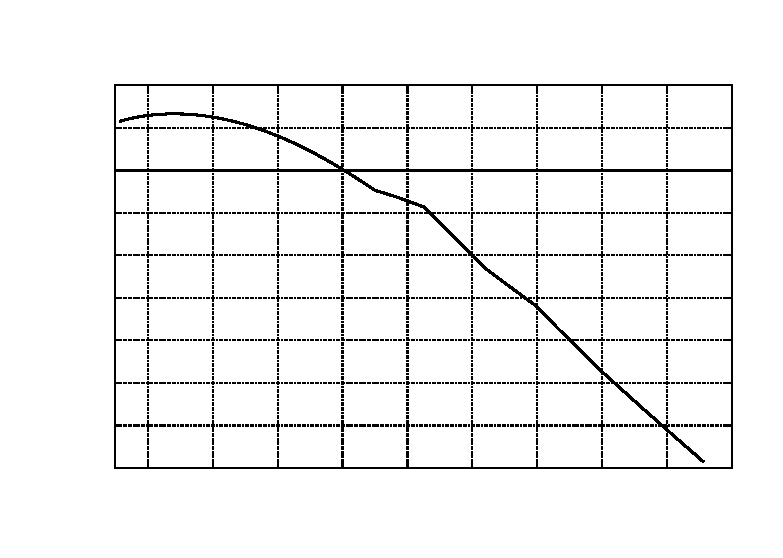
\includegraphics{../graphs/efis_ias_err_flaps_up}}%
    \gplfronttext
  \end{picture}%
\endgroup
\end{center}  % for gnuplot epslatex, latex or pslatex mode
}
\caption{EFIS Airspeed Error --- Airspeed --- Flaps Retracted}
\label{EFIS-spd-error}
\end{figure}


    % EFIS Airspeed Error Chart --- Static Source Position Error + EFIS ASI inst error
% EFIS ASI TAS Correction Table
\begin{figure}[t]
% \addcontentsline{toc}{section}{Figure \ref{TO-Dist} Takeoff Distance}
\addcontentsline{toc}{section}{EFIS ASI TAS CORRECTION}
\begin{center}
\begin{perfhdr}EFIS ASI TAS CORRECTION\\
1800 LBS
\end{perfhdr}
\Large
% \textcolor{red}{VANS CLAIMED PERF EXPANDED TO OTHER CONDITIONS}\vspace{1ex}\\
% \textcolor{red}{TO BE CONFIRMED BY FLIGHT TEST}\normalsize \vspace{5ex}\\

% \begin{minipage}{7.5in}
%   \begin{flushleft}
%     CONDITIONS:\\
%     Flaps 17\textdegree \ (set flap angle to match down aileron angle at full aileron)\\
%     2700 RPM, Full Throttle and Mixture Set prior to Brake Release\\
%     Paved, Level, Dry Runway\\
%     Zero Wind\\
% \vspace{\perfnoteskip}
%     NOTES:
%     \begin{enumerate*}
%       \item Short field technique as specified in Section \textcolor{red}{4}.
% %      \item Prior to takeoff from fields above 8,000 ft elevation, the mixture should be leaned to give maximum power in
% %      a full throttle static runup.
%       \item Set mixture at placard fuel flow.
%       \item Decrease distance by 10\% for each \textcolor{red}{X} knots headwind.  For operations with tailwinds up to 10
%       knots, increase distances by \textcolor{red}{10\%}.
%       \item For operation on a dry, grass runway, increase distances by \textcolor{red}{10\%} of the ground roll figure.
%       \end{enumerate*}
%     \end{flushleft}
%   \end{minipage}
% \hfill
% \begin{minipage}{1.5in}
%   \begin{tabular}{|c|c|}
%     \hline
%     \multicolumn{2}{|c|}{MIXTURE SETTING}\\
%     \hline
%     PRESS ALT&GPH\\
%     \hline
%     S.L.&17\\
%     2000&16\\
%     4000&15\\
%     6000&14\\
%     8000&13\\
%     \hline
%     \end{tabular}
%   \end{minipage}
% \\
\vspace{\perfnoteskip}
    \raggedright NOTES:
    \begin{enumerate*}
      \item Table provides TAS correction as a function of altitude and IAS.
      \item Corrected TAS = TAS displayed on EFIS + correction.
      \item Table includes static source position error, EFIS ASI instrument error and OAT ram temperature rise.
      \end{enumerate*}

\vspace{\perfnoteskip}
\settowidth{\colOne}{ALTITUDE}
% \settowidth{\colFive}{GRND}
\begin{tabular}{|c|c|c|c|c|c|c|c|c|c|c|c|}
\hline
\multirow{2}{\colOne}{\centering ALTITUDE (FT)}&\multicolumn{11}{c|}{IAS (KT)}\\
\cline{2-12}
&80&90&100&110&120&130&140&150&160&170&180\\
\hline
\hline
0&+1.2&+1.0&+0.8&+0.4&+0.0&-0.5&-0.7&-1.3&-2.1&-2.9&-3.6\\
\hline
5,000&+1.3&+1.1&+0.8&+0.4&-0.0&-0.6&-0.9&-1.5&-2.4&-3.2&-4.0\\
\hline
10,000&+1.3&+1.1&+0.8&+0.4&-0.1&-0.7&-1.0&-1.7&-2.7&-3.6&-4.5\\
\hline
15,000&+1.4&+1.2&+0.9&+0.4&-0.2&-0.8&-1.3&-2.0&-3.1&-4.2&-5.1\\
\hline
20,000&+1.5&+1.3&+0.9&+0.3&-0.3&-1.1&-1.5&-2.4&-3.6&-4.8&-5.8\\
\hline
&\multicolumn{11}{c|}{TAS CORRECTION (KT)}\\
\hline
\end{tabular}
\end{center}
\caption{EFIS ASI TAS Correction}
\label{EFIS-ASI-TAS-Corr}
\end{figure}

      % EFIS ASI TAS Correction Table
% Stall Speed Chart
\begin{figure}[t]
% \addcontentsline{toc}{section}{Figure \ref{stall-speed-kcas} Stall Speed --- KCAS}
\addcontentsline{toc}{section}{STALL SPEED --- KCAS}
\begin{center}
\begin{perfhdr}STALL SPEED --- KCAS\\
\end{perfhdr}

\begin{minipage}{2in}
  \begin{flushleft}
    CONDITIONS:\\
    Idle power\\
    Prop control at Max RPM\\
    Deceleration at 1 kt/s\\
    \end{flushleft}
  \end{minipage}\\
%\vspace{2ex}
% GNUPLOT: LaTeX picture with Postscript
\begingroup
  \makeatletter
  \providecommand\color[2][]{%
    \GenericError{(gnuplot) \space\space\space\@spaces}{%
      Package color not loaded in conjunction with
      terminal option `colourtext'%
    }{See the gnuplot documentation for explanation.%
    }{Either use 'blacktext' in gnuplot or load the package
      color.sty in LaTeX.}%
    \renewcommand\color[2][]{}%
  }%
  \providecommand\includegraphics[2][]{%
    \GenericError{(gnuplot) \space\space\space\@spaces}{%
      Package graphicx or graphics not loaded%
    }{See the gnuplot documentation for explanation.%
    }{The gnuplot epslatex terminal needs graphicx.sty or graphics.sty.}%
    \renewcommand\includegraphics[2][]{}%
  }%
  \providecommand\rotatebox[2]{#2}%
  \@ifundefined{ifGPcolor}{%
    \newif\ifGPcolor
    \GPcolorfalse
  }{}%
  \@ifundefined{ifGPblacktext}{%
    \newif\ifGPblacktext
    \GPblacktexttrue
  }{}%
  % define a \g@addto@macro without @ in the name:
  \let\gplgaddtomacro\g@addto@macro
  % define empty templates for all commands taking text:
  \gdef\gplbacktext{}%
  \gdef\gplfronttext{}%
  \makeatother
  \ifGPblacktext
    % no textcolor at all
    \def\colorrgb#1{}%
    \def\colorgray#1{}%
  \else
    % gray or color?
    \ifGPcolor
      \def\colorrgb#1{\color[rgb]{#1}}%
      \def\colorgray#1{\color[gray]{#1}}%
      \expandafter\def\csname LTw\endcsname{\color{white}}%
      \expandafter\def\csname LTb\endcsname{\color{black}}%
      \expandafter\def\csname LTa\endcsname{\color{black}}%
      \expandafter\def\csname LT0\endcsname{\color[rgb]{1,0,0}}%
      \expandafter\def\csname LT1\endcsname{\color[rgb]{0,1,0}}%
      \expandafter\def\csname LT2\endcsname{\color[rgb]{0,0,1}}%
      \expandafter\def\csname LT3\endcsname{\color[rgb]{1,0,1}}%
      \expandafter\def\csname LT4\endcsname{\color[rgb]{0,1,1}}%
      \expandafter\def\csname LT5\endcsname{\color[rgb]{1,1,0}}%
      \expandafter\def\csname LT6\endcsname{\color[rgb]{0,0,0}}%
      \expandafter\def\csname LT7\endcsname{\color[rgb]{1,0.3,0}}%
      \expandafter\def\csname LT8\endcsname{\color[rgb]{0.5,0.5,0.5}}%
    \else
      % gray
      \def\colorrgb#1{\color{black}}%
      \def\colorgray#1{\color[gray]{#1}}%
      \expandafter\def\csname LTw\endcsname{\color{white}}%
      \expandafter\def\csname LTb\endcsname{\color{black}}%
      \expandafter\def\csname LTa\endcsname{\color{black}}%
      \expandafter\def\csname LT0\endcsname{\color{black}}%
      \expandafter\def\csname LT1\endcsname{\color{black}}%
      \expandafter\def\csname LT2\endcsname{\color{black}}%
      \expandafter\def\csname LT3\endcsname{\color{black}}%
      \expandafter\def\csname LT4\endcsname{\color{black}}%
      \expandafter\def\csname LT5\endcsname{\color{black}}%
      \expandafter\def\csname LT6\endcsname{\color{black}}%
      \expandafter\def\csname LT7\endcsname{\color{black}}%
      \expandafter\def\csname LT8\endcsname{\color{black}}%
    \fi
  \fi
  \setlength{\unitlength}{0.0500bp}%
  \begin{picture}(7200.00,5040.00)%
    \gplgaddtomacro\gplbacktext{%
      \csname LTb\endcsname%
      \put(1078,704){\makebox(0,0)[r]{\strut{} 1300}}%
      \csname LTb\endcsname%
      \put(1078,1383){\makebox(0,0)[r]{\strut{} 1400}}%
      \csname LTb\endcsname%
      \put(1078,2061){\makebox(0,0)[r]{\strut{} 1500}}%
      \csname LTb\endcsname%
      \put(1078,2740){\makebox(0,0)[r]{\strut{} 1600}}%
      \csname LTb\endcsname%
      \put(1078,3418){\makebox(0,0)[r]{\strut{} 1700}}%
      \csname LTb\endcsname%
      \put(1078,4097){\makebox(0,0)[r]{\strut{} 1800}}%
      \csname LTb\endcsname%
      \put(1078,4775){\makebox(0,0)[r]{\strut{} 1900}}%
      \csname LTb\endcsname%
      \put(1210,484){\makebox(0,0){\strut{} 45}}%
      \csname LTb\endcsname%
      \put(2608,484){\makebox(0,0){\strut{} 50}}%
      \csname LTb\endcsname%
      \put(4007,484){\makebox(0,0){\strut{} 55}}%
      \csname LTb\endcsname%
      \put(5405,484){\makebox(0,0){\strut{} 60}}%
      \csname LTb\endcsname%
      \put(6803,484){\makebox(0,0){\strut{} 65}}%
      \put(176,2739){\rotatebox{-270}{\makebox(0,0){\strut{}Gross Weight (lb)}}}%
      \put(4006,154){\makebox(0,0){\strut{}Stall Speed (KCAS)}}%
      \put(3028,2740){\rotatebox{57}{\makebox(0,0)[l]{\strut{}Full Flap}}}%
      \put(4146,2061){\rotatebox{52}{\makebox(0,0)[l]{\strut{}Flaps UP}}}%
    }%
    \gplgaddtomacro\gplfronttext{%
    }%
    \gplbacktext
    \put(0,0){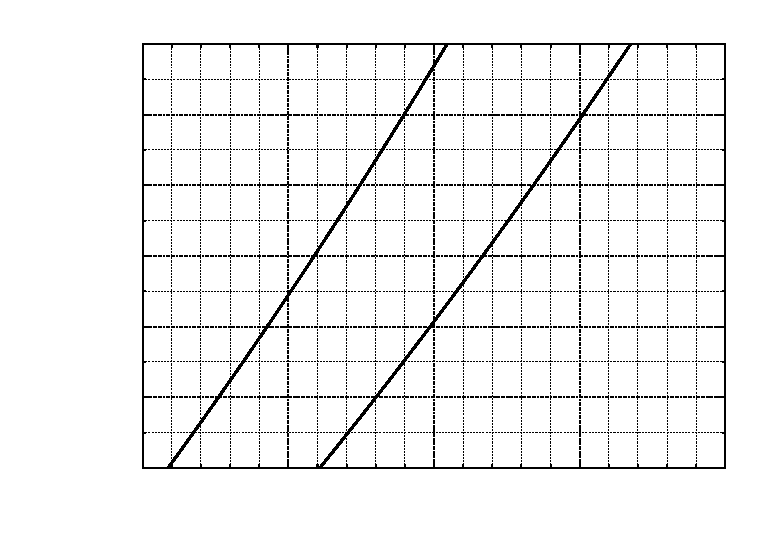
\includegraphics{../graphs/stall}}%
    \gplfronttext
  \end{picture}%
\endgroup
\end{center}  % for gnuplot epslatex, latex or pslatex mode
\caption{Stall Speed --- KCAS}
\label{stall-speed-kcas}
\end{figure}
\clearpage


            % Stall Speed Chart
% Takeoff Performance
\begin{sidewaysfigure}[t]
% \addcontentsline{toc}{section}{Figure \ref{TO-Dist} Takeoff Distance}
\addcontentsline{toc}{section}{TAKEOFF DISTANCE}
\begin{center}
\begin{perfhdr}TAKEOFF DISTANCE\\
1800 LBS
\end{perfhdr}
\Large
\textcolor{red}{VANS CLAIMED PERF EXPANDED TO OTHER CONDITIONS}\vspace{1ex}\\
\textcolor{red}{TO BE CONFIRMED BY FLIGHT TEST}\normalsize \vspace{5ex}\\

\begin{minipage}{7.5in}
  \begin{flushleft}
    CONDITIONS:\\
    Flaps 17\textdegree \ (set flap angle to match down aileron angle at full aileron)\\
    2700 RPM, Full Throttle and Mixture Set prior to Brake Release\\
    Paved, Level, Dry Runway\\
    Zero Wind\\
\vspace{\perfnoteskip}
    NOTES:
    \begin{enumerate*}
      \item Short field technique as specified in Section \textcolor{red}{4}.
%      \item Prior to takeoff from fields above 8,000 ft elevation, the mixture should be leaned to give maximum power in
%      a full throttle static runup.
      \item Set mixture at placard fuel flow.
      \item Decrease distance by 10\% for each \textcolor{red}{X} knots headwind.  For operations with tailwinds up to 10
      knots, increase distances by \textcolor{red}{10\%}.
      \item For operation on a dry, grass runway, increase distances by \textcolor{red}{10\%} of the ground roll figure.
      \end{enumerate*}
    \end{flushleft}
  \end{minipage}
\hfill
\begin{minipage}{1.5in}
  \begin{tabular}{|c|c|}
    \hline
    \multicolumn{2}{|c|}{MIXTURE SETTING}\\
    \hline
    PRESS ALT&GPH\\
    \hline
    S.L.&17\\
    2000&16\\
    4000&15\\
    6000&14\\
    8000&13\\
    \hline
    \end{tabular}
  \end{minipage}
\\

\vspace{\perfnoteskip}
\settowidth{\colOne}{WEIGHT}
\settowidth{\colFive}{GRND}
\begin{tabular}{|c|c|c|r|r|r|r|r|r|r|r|r|r|r|}
\hline
\multirow{5}{\colOne}{\centering WEIGHT (LB)}&\multicolumn{2}{c|}{TAKEOFF}&&\multicolumn{2}{c|}{0\textdegree C}&\multicolumn{2}{c|}{10\textdegree C}&\multicolumn{2}{c|}{20\textdegree C}&\multicolumn{2}{c|}{30\textdegree C}&\multicolumn{2}{c|}{40\textdegree C}\\
\cline{5-14}
&\multicolumn{2}{c|}{SPEED}&\multicolumn{1}{c|}{PRESS}&\multirow{4}{\colFive}{\centering GRND ROLL (FT)}&
\multicolumn{1}{c|}{TOTAL}&\multirow{4}{\colFive}{\centering GRND ROLL (FT)}&
\multicolumn{1}{c|}{TOTAL}&\multirow{4}{\colFive}{\centering GRND ROLL (FT)}&
\multicolumn{1}{c|}{TOTAL}&\multirow{4}{\colFive}{\centering GRND ROLL (FT)}&
\multicolumn{1}{c|}{TOTAL}&\multirow{4}{\colFive}{\centering GRND ROLL (FT)}&\multicolumn{1}{c|}{TOTAL}\\
&\multicolumn{2}{c|}{(KIAS)}&\multicolumn{1}{c|}{ALT}&&\multicolumn{1}{c|}{DIST}&&
\multicolumn{1}{c|}{DIST}&&\multicolumn{1}{c|}{DIST}&&\multicolumn{1}{c|}{DIST}&&\multicolumn{1}{c|}{DIST}\\
\cline{2-3}
&LIFT&AT&\multicolumn{1}{c|}{(FT)}&&\multicolumn{1}{c|}{TO}&&\multicolumn{1}{c|}{TO}&&
\multicolumn{1}{c|}{TO}&&\multicolumn{1}{c|}{TO}&&\multicolumn{1}{c|}{TO}\\
&OFF&50 FT&&&\multicolumn{1}{c|}{50 FT}&&\multicolumn{1}{c|}{50 FT}&&\multicolumn{1}{c|}{50 FT}&&\multicolumn{1}{c|}{50 FT}&&\multicolumn{1}{c|}{50 FT}\\
\hline
\hline

1800&XX&YY&S.L.&460&TTT&490&TTT&510&TTT&550&TTT&580&TTT\\
\hline
&XX&YY&2,000&550&TTT&590&TTT&620&TTT&660&TTT&700&TTT\\
\hline
&XX&YY&4,000&670&TTT&710&TTT&750&TTT&800&TTT&840&TTT\\
\hline
&XX&YY&6,000&810&TTT&860&TTT&920&TTT&970&TTT&1020&TTT\\
\hline
&XX&YY&8,000&990&TTT&1050&TTT&1120&TTT&1180&TTT&1250&TTT\\
\hline
&XX&YY&10,000&1210&TTT&1280&TTT&1360&TTT&1440&TTT&1520&TTT\\
\hline
&XX&YY&12,000&1480&TTT&1570&TTT&1670&TTT&1770&TTT&1870&TTT\\
\hline
\end{tabular}
\end{center}
\caption{Takeoff Distance}
\label{TO-Dist}
\end{sidewaysfigure}

                % Takeoff Performance
% Rate of Climb Chart
\begin{figure}[t]
% \addcontentsline{toc}{section}{Figure \ref{ROC-Max} Rate of Climb --- Maximum Power}
\addcontentsline{toc}{section}{RATE OF CLIMB --- MAXIMUM POWER}
\begin{center}
\begin{perfhdr}RATE OF CLIMB
\end{perfhdr}
\Large
\textcolor{red}{DATA TO BE CONFIRMED BY FLIGHT TEST}\normalsize \\
\vspace{5ex}
\begin{minipage}{4in}
  \begin{flushleft}
    CONDITIONS:\\
    Flaps UP\\
    2700 RPM\\
    Full Throttle\\
    Mixture Set at Placard Fuel Flow
%    NOTE:
%    Mixture leaned when power is at 75\% power or less (8,000 ft or above at standard temperature) for smooth
%    engine operation and increased power.
    \end{flushleft}
  \end{minipage}
\hfill
\begin{minipage}{1.5in}
  \begin{tabular}{|c|c|}
    \hline
    \multicolumn{2}{|c|}{MIXTURE SETTING}\\
    \hline
    PRESS ALT&GPH\\
    \hline
    S.L.&17\\
    2000&16\\
    4000&15\\
    6000&14\\
    8000&13\\
    \hline
    \end{tabular}
  \end{minipage}
\\
\vspace{\perfnoteskip}

\settowidth{\colOne}{WEIGHT}
\settowidth{\colTwo}{PRESSURE}
\settowidth{\colThree}{CLIMB}
\settowidth{\colFour}{-20\textdegree C}
\settowidth{\colFive}{9,999}
\settowidth{\colSix}{9,999}
\settowidth{\colSeven}{9,999}

\begin{tabular}{|c|r|r|r|r|r|r|}
\hline
\multirow{3}{\colOne}{\centering WEIGHT (LB)}&\multirow{3}{\colTwo}{\centering PRESSURE ALTITUDE (FT)}&
\multirow{3}{\colThree}{\centering CLIMB SPEED (KIAS)}&
\multicolumn{4}{c|}{RATE OF CLIMB (FT/MN)}\\
\cline{4-7}
&&&\multirow{2}{\colFour}{\centering -20\textdegree C}&\multirow{2}{\colFive}{\centering 0\textdegree C}&
\multirow{2}{\colSix}{\centering 20\textdegree C}&\multirow{2}{\colSeven}{\centering 40\textdegree C}\\
&&&&&&\\
\hline
\hline
1800&0&99&2190&2100&2010&1910\\
\hline
&2,000&96&1980&1890&1800&1700\\
\hline
&4,000&93&1770&1690&1600&1510\\
\hline
&6,000&91&1570&1490&1400&1320\\
\hline
&8,000&90&1380&1300&1210&1130\\
\hline
&10,000&88&1190&1110&1030&950\\
\hline
&12,000&87&1010&930&860&780\\
\hline
&14,000&86&840&760&690&620\\
\hline
&16,000&84&670&590&520&450\\
\hline
&18,000&83&500&430&360&290\\
\hline
&20,000&82&340&260&190&120\\
\hline
\end{tabular}
\end{center}
\caption{Rate of Climb --- Maximum Power}
\label{ROC-Max}
\end{figure}


                    % Rate of Climb Chart
% Time, Fuel and Distance to Climb table --- Max Power
\begin{figure}[t]
% \addcontentsline{toc}{section}{Figure \ref{TFD-to-climb-Max} Time, Fuel and Distance to Climb --- Maximum Power}
\addcontentsline{toc}{section}{TIME, FUEL AND DISTANCE TO CLIMB --- MAXIMUM POWER}
\begin{center}
\begin{perfhdr}TIME, FUEL AND DISTANCE TO CLIMB\\
MAXIMUM POWER\\
\end{perfhdr}
\Large
% \textcolor{red}{DATA TO BE CONFIRMED BY FLIGHT TEST}\\
\normalsize \vspace{5ex} 
\raggedright 
    CONDITIONS:\\
    Flaps UP\\
    2650 RPM\\
    Full Throttle\\
    Mixture Set to give EGT 25\textdegree F less than EGT during take-off\\
    Standard Temperature\\

\hfill

\vspace{\perfnoteskip}
    \raggedright NOTES:
    \begin{enumerate*}
      \item Add 1.0 USG of fuel for engine start, taxi and takeoff.
%      \item Mixture leaned when power is at 75\% power or less (8,000 ft or above at standard temperature) for smooth
%      engine operation and increased power.
      \item Climb speed is 102 KIAS at sea level, decreasing by 1 kt per 1000 ft.
      \item Increase time, fuel and distance by 10\% for each 10\textdegree C above standard
      temperatures.
      \item Distances shown are based on zero wind.
      \end{enumerate*}

\vspace{\perfnoteskip}
% following lengths are used to set row widths to fit the text
\settowidth{\colOne}{WEIGHT}
\settowidth{\colTwo}{PRESS.}
\settowidth{\colThree}{TEMP}
\settowidth{\colFour}{CLIMB}
\settowidth{\colFive}{RATE OF}
\settowidth{\colSix}{TIME}
\settowidth{\colSeven}{USED}
\settowidth{\colEight}{DIST.}

\begin{tabular}{|c|r|r|r|r|r|r|r|}
\hline
\multirow{3}{\colOne}[\halfrowdrop]{\centering WEIGHT (LB)}&\multirow{3}{\colTwo}[\halfrowdrop]{\centering PRESS. ALT. (FT)}&
\multirow{3}{\colThree}[\halfrowdrop]{\centering TEMP (\textdegree C)}&\multirow{3}{\colFour}[\halfrowdrop]{\centering CLIMB SPEED (KIAS)}&
\multirow{3}{\colFive}[\halfrowdrop]{\centering RATE OF CLIMB (FT/MN)}&\multicolumn{3}{c|}{FROM SEA LEVEL}\\
\cline{6-8}
&&&&&\multicolumn{1}{m{\colSix}|}{\centering TIME (MN)}&\multicolumn{1}{m{\colSeven}|}{\centering FUEL USED (USG)}&\multicolumn{1}{m{\colEight}|}{\centering DIST. (NM)}\\
\hline
\hline
% % START of copied data from python Climb_DA_fit.py script
% % Based on climb tests on flights 261, 262, 263 & 264
1,800&0&15&102&1,810&0&0&0\\
\hline
&2,000&11&100&1,640&1&0.3&2\\
\hline
&4,000&7&98&1,470&2&0.7&4\\
\hline
&6,000&3&96&1,300&4&1.0&7\\
\hline
&8,000&-1&94&1,130&6&1.4&10\\
\hline
&10,000&-5&92&960&7&1.8&13\\
\hline
&12,000&-9&90&790&10&2.3&17\\
\hline
&14,000&-13&90&620&13&2.9&22\\
\hline
&16,000&-17&90&450&16&3.5&29\\
\hline
&18,000&-21&90&290&22&4.5&40\\
\hline
&20,000&-25&90&120&32&6.1&60\\
\hline
% % END of copied data from python Climb_DA_fit.py script
\end{tabular}
\end{center}
\caption{Time, Fuel and Distance to Climb --- Maximum Power}
\label{TFD-to-climb-Max}
\end{figure}



         % Time, Fuel and Distance to Climb table --- Max Power
% % Time, Fuel and Distance to Climb table --- Normal Climb Power
\begin{figure}[t]
% \addcontentsline{toc}{section}{Figure \ref{TFD-to-climb-Norm} Time, Fuel and Distance to Climb --- Normal Climb Power}
\addcontentsline{toc}{section}{TIME, FUEL AND DISTANCE TO CLIMB --- NORMAL CLIMB POWER}
\begin{center}
\begin{perfhdr}TIME, FUEL AND DISTANCE TO CLIMB\\
NORMAL CLIMB\\
\end{perfhdr}
\Large
% \textcolor{red}{DATA TO BE CONFIRMED BY FLIGHT TEST}\\
\normalsize
\vspace{5ex}
\begin{minipage}{4in}
  \begin{flushleft}
    CONDITIONS:\\
    Flaps UP\\
    2650 RPM\\
    Full Throttle\\
    Mixture Set at Indicated Fuel Flow
    Standard Temperature\\
    \end{flushleft}
\end{minipage}
\hfill
\begin{minipage}{1.5in}
  \begin{tabular}{|c|c|}
    \hline
    \multicolumn{2}{|c|}{MIXTURE SETTING}\\
    \hline
    PRESS ALT&GPH\\
    \hline
    S.L.&17\\
    2000&16\\
    4000&15\\
    6000&14\\
    8000&13\\
    10,000&12.5\\
    12,000&11.8\\
    14,000&11.1\\
    16,000&10.4\\
    \hline
    \end{tabular}
  \end{minipage}
\\
\vspace{\perfnoteskip}
    \raggedright NOTES:
    \begin{enumerate*}
      \item Add 1.5 USG of fuel for engine start, taxi and takeoff.
%      \item Mixture leaned when power is at 75\% power or less (6,000 ft or above at standard temperature) for smooth engine operation and increased power.
      \item Climb speed is 100 KIAS from sea level to 10,000 ft, then decreasing by 2 kt per 1000 ft above 10,000 ft.
      \item Increase time, fuel and distance by \textcolor{red}{XX\%} for each 10\textdegree C above standard temperatures.
      \item Distances shown are based on zero wind.
      \end{enumerate*}
\vspace{\perfnoteskip}
% following lengths are used to set row widths to fit the text
\settowidth{\colOne}{WEIGHT}
\settowidth{\colTwo}{PRESSURE}
\settowidth{\colThree}{TEMP}
\settowidth{\colFour}{CLIMB}
\settowidth{\colFive}{RATE OF}
\settowidth{\colSix}{TIME}
\settowidth{\colSeven}{USED}
\settowidth{\colEight}{DIST.}

\begin{tabular}{|c|r|r|r|r|r|r|r|}
\hline
\multirow{3}{\colOne}[\halfrowdrop]{\centering WEIGHT (LB)}&\multirow{3}{\colTwo}[\halfrowdrop]{\centering PRESSURE ALTITUDE (FT)}&
\multirow{3}{\colThree}[\halfrowdrop]{\centering TEMP (\textdegree C)}&\multirow{3}{\colFour}[\halfrowdrop]{\centering CLIMB SPEED (KIAS)}&
\multirow{3}{\colFive}[\halfrowdrop]{\centering RATE OF CLIMB (FT/MN)}&\multicolumn{3}{c|}{FROM SEA LEVEL}\\
\cline{6-8}
&&&&&\multicolumn{1}{m{\colSix}|}{\centering TIME (MN)}&\multicolumn{1}{m{\colSeven}|}{\centering FUEL USED (USG)}&\multicolumn{1}{m{\colEight}|}{\centering DIST. (NM)}\\
\hline
\hline
% % START of copied data from python perf script
% % Data use 95% of the calculated power to match the results from the flight test with the test the Hartzell prop
1800&0&15&100&1630&0&0&0\\
\hline
&2,000&11&100&1480&1&0.3&2\\
\hline
&4,000&7&100&1320&3&0.6&5\\
\hline
&6,000&3&100&1170&4&0.9&8\\
\hline
&8,000&-1&100&1020&6&1.2&11\\
\hline
&10,000&-5&100&870&8&1.6&15\\
\hline
&12,000&-9&96&750&11&2.0&20\\
\hline
&14,000&-13&92&620&14&2.5&25\\
\hline
&16,000&-17&88&500&17&3.0&32\\
\hline
&18,000&-21&84&380&22&3.7&41\\
\hline
&20,000&-25&80&250&28&4.5&52\\
\hline
% % END of copied data from python perf script
\end{tabular}
\end{center}
\caption{Time, Fuel and Distance to Climb --- Normal Climb Power}
\label{TFD-to-climb-Norm}
\end{figure}


        % Time, Fuel and Distance to Climb table --- Normal Climb Power
% Time, Fuel and Distance to Climb table --- Normal Climb Power
\begin{figure}[t]
% \addcontentsline{toc}{section}{Figure \ref{TFD-to-climb-Norm} Time, Fuel and Distance to Climb --- Normal Climb Power}
\addcontentsline{toc}{section}{TIME, FUEL AND DISTANCE TO CLIMB --- CRUISE CLIMB}
\begin{center}
\begin{perfhdr}TIME, FUEL AND DISTANCE TO CLIMB\\
CRUISE CLIMB\\
\end{perfhdr}
\Large
% \textcolor{red}{DATA TO BE CONFIRMED BY FLIGHT TEST}\\
\normalsize
\vspace{5ex}
    \raggedright 
    CONDITIONS:\\
    Flaps UP\\
    2500 RPM\\
    Full Throttle\\
    Mixture Set to give EGT 25\textdegree F less than EGT during take-off\\
    Standard Temperature\\
\hfill

\vspace{\perfnoteskip}
    \raggedright NOTES:
    \begin{enumerate*}
      \item Add 1.5 USG of fuel for engine start, taxi and takeoff.
%      \item Mixture leaned when power is at 75\% power or less (6,000 ft or above at standard temperature) for smooth engine operation and increased power.
      \item Climb speed is 120 KIAS from sea level to 10,000 ft, then decreasing by 4 kt per 1000 ft above 10,000 ft.
      \item Increase time, fuel and distance by \textcolor{red}{XX\%} for each 10\textdegree C above standard temperatures.
      \item Distances shown are based on zero wind.
      \end{enumerate*}
\vspace{\perfnoteskip}
% following lengths are used to set row widths to fit the text
\settowidth{\colOne}{WEIGHT}
\settowidth{\colTwo}{PRESSURE}
\settowidth{\colThree}{TEMP}
\settowidth{\colFour}{CLIMB}
\settowidth{\colFive}{RATE OF}
\settowidth{\colSix}{TIME}
\settowidth{\colSeven}{USED}
\settowidth{\colEight}{DIST.}

\begin{tabular}{|c|r|r|r|r|r|r|r|}
\hline
\multirow{3}{\colOne}[\halfrowdrop]{\centering WEIGHT (LB)}&\multirow{3}{\colTwo}[\halfrowdrop]{\centering PRESSURE ALTITUDE (FT)}&
\multirow{3}{\colThree}[\halfrowdrop]{\centering TEMP (\textdegree C)}&\multirow{3}{\colFour}[\halfrowdrop]{\centering CLIMB SPEED (KIAS)}&
\multirow{3}{\colFive}[\halfrowdrop]{\centering RATE OF CLIMB (FT/MN)}&\multicolumn{3}{c|}{FROM SEA LEVEL}\\
\cline{6-8}
&&&&&\multicolumn{1}{m{\colSix}|}{\centering TIME (MN)}&\multicolumn{1}{m{\colSeven}|}{\centering FUEL USED (USG)}&\multicolumn{1}{m{\colEight}|}{\centering DIST. (NM)}\\
\hline
\hline
% % START of copied data from python perf script
1,800&0&15&120&1,540&0&0&0\\
\hline
&2,000&11&120&1,340&1&0.3&3\\
\hline
&4,000&7&120&1,160&3&0.6&6\\
\hline
&6,000&3&120&980&5&1.0&10\\
\hline
&8,000&-1&120&780&7&1.4&15\\
\hline
&10,000&-5&120&580&10&1.9&22\\
\hline
&12,000&-9&112&520&14&2.5&30\\
\hline
&14,000&-13&104&430&18&3.1&39\\
\hline
&16,000&-17&96&340&23&3.8&50\\
\hline
&18,000&-21&88&220&30&4.8&64\\
\hline
&20,000&-25&80&90&43&6.3&89\\
\hline
% % END of copied data from python perf script
\end{tabular}
\end{center}
\caption{Time, Fuel and Distance to Climb --- Normal Climb Power}
\label{TFD-to-climb-Norm}
\end{figure}


        % Time, Fuel and Distance to Climb table --- Cruise Climb
% Cruise Power Chart 
% Fuel Flow vs power from Lycoming Operator's Manual Curve 12699B, pg 3-22, converted
% from lb/hr to USG/hr using 6.01 lb/USG
\settowidth{\colOne}{PRESSURE}
\settowidth{\colTwo}{FLOW}
\settowidth{\colThree}{BEST POWER}

\begin{sidewaysfigure}[t]
% \addcontentsline{toc}{section}{Figure \ref{Cruise-power} Cruise Power}
\addcontentsline{toc}{section}{CRUISE POWER}
\begin{center}
\begin{perfhdr}CRUISE POWER
\end{perfhdr}
%\vspace{5ex}
\begin{minipage}{9in}
\begin{minipage}{5in}
NOTES:
\begin{enumerate*}
\item Add 0.4" M.P. for each 10\textdegree C above standard temperature.  
\item Subtract 0.4" M.P. for each 10\textdegree C below standard temperature.
\item If above standard temperature precludes obtaining the desired M.P., use the next higher RPM/M.P. with appropriate temperature correction to M.P.
\end{enumerate*}

\end{minipage}
\hfill
\begin{boxedminipage}{3in}
\begin{center}NOTE\end{center}
Mixture must be full rich when above 75\% power. Lean using fuel flow meter at 75\% power or less.
\end{boxedminipage}
\end{minipage}\\
\vspace{\perfnoteskip}
%\small
\begin{tabular}{|r|cc||c|c|c|c||c|c|c|c||c|c|c|c|c|}
\hline
&&&\multicolumn{4}{c||}{75\% POWER}&\multicolumn{4}{c||}{65\% POWER}&\multicolumn{5}{c|}{55\% POWER}\\
&&&\multicolumn{4}{c||}{150 HP}&\multicolumn{4}{c||}{130 HP}&\multicolumn{5}{c|}{110 HP}\\
\hline
\multirow{4}{\colOne}{\centering PRESSURE ALTITUDE (FT)}&\multicolumn{2}{r||}{RPM}&
2400&2500&2600&2700&2300&2400&2500&2600&2200&2300&2400&2500&2600\\
\cline{2-16}
&\multirow{2}{\colTwo}{\centering FUEL FLOW}&\multicolumn{1}{|l||}{BEST ECON.}& 9.9& 10.0&10.2& 10.3& 8.7& 8.8& 8.9& 9.0& 7.4&7.5& 7.6& 7.8& 7.9& \\
&&\multicolumn{1}{|l||}{BEST POWER}& 11.8& 11.9&12.1& 12.2& 10.3& 10.4& 10.6& 10.7& 8.9&9.0& 9.2& 9.4& 9.6& \\
\cline{2-16}
&\multicolumn{2}{c||}{STD. TEMP}&\multicolumn{4}{c||}{MANIFOLD PRESS.}&\multicolumn{4}{c||}{MANIFOLD PRESS.}&\multicolumn{5}{c|}{MANIFOLD PRESS.}\\
\hline
\hline
0&\multicolumn{2}{c||}{15 \textdegree C}&25.4&24.5&23.6&22.8&23.7&22.8&22.0&21.2&22.0&21.0&20.2&19.5&18.9\\
\hline
2,000&\multicolumn{2}{c||}{11 \textdegree C}&24.9&23.9&23.1&22.3&23.2&22.3&21.5&20.7&21.5&20.5&19.7&19.0&18.4\\
\hline
4,000&\multicolumn{2}{c||}{7 \textdegree C}&24.4&23.4&22.6&21.9&22.7&21.8&21.0&20.3&21.0&20.0&19.3&18.5&17.9\\
\hline
6,000&\multicolumn{2}{c||}{3 \textdegree C}&23.9&23.0&22.1&21.5&22.3&21.4&20.5&19.8&20.5&19.6&18.9&18.1&17.5\\
\hline
8,000&\multicolumn{2}{c||}{-1 \textdegree C}&23.5&22.5&21.7&21.1&21.9&21.0&20.1&19.4&20.1&19.2&18.5&17.7&17.1\\
\hline
10,000&\multicolumn{2}{c||}{-5 \textdegree C}&--&--&--&--&21.5&20.6&19.7&19.0&19.7&18.9&18.1&17.3&16.7\\
\hline
12,000&\multicolumn{2}{c||}{-9 \textdegree C}&--&--&--&--&--&20.2&19.3&18.7&19.3&18.5&17.7&16.9&16.4\\
\hline

\end{tabular}
\normalsize 
\end{center}
\caption{Cruise Power}
\label{Cruise-power}
\end{sidewaysfigure}


             % Cruise Power Chart 
% Cruise Speed Chart - Wheel Pants ON
\begin{figure}[t]
% \addcontentsline{toc}{section}{Figure \ref{Cruise-speed} Cruise Speed}
\addcontentsline{toc}{section}{CRUISE SPEED}
\begin{center}
\begin{perfhdr}CRUISE SPEED\\
\end{perfhdr}

\begin{minipage}{5in}
  \begin{flushleft}
    CONDITIONS:\\
    Wheel Pants and Gear Leg Fairings ON\\
    Standard atmosphere.\\
    Mixture set to best power for 75\% power.\\
    Mixture set to 50\textdegree F lean of peak EGT for 65\% and 55\% power, except mixture set to best power if more than 2600 rpm required with mixture set lean of peak EGT.\\
    Full throttle, but no less than 2100 rpm.\\
    Speed vs RPM lines are at full throttle, with mixture set to best power or 50 deg F Lean of Peak EGT.
    \end{flushleft}
\end{minipage}\\
\vspace{5ex}

% GNUPLOT: LaTeX picture with Postscript
\begingroup
  \makeatletter
  \providecommand\color[2][]{%
    \GenericError{(gnuplot) \space\space\space\@spaces}{%
      Package color not loaded in conjunction with
      terminal option `colourtext'%
    }{See the gnuplot documentation for explanation.%
    }{Either use 'blacktext' in gnuplot or load the package
      color.sty in LaTeX.}%
    \renewcommand\color[2][]{}%
  }%
  \providecommand\includegraphics[2][]{%
    \GenericError{(gnuplot) \space\space\space\@spaces}{%
      Package graphicx or graphics not loaded%
    }{See the gnuplot documentation for explanation.%
    }{The gnuplot epslatex terminal needs graphicx.sty or graphics.sty.}%
    \renewcommand\includegraphics[2][]{}%
  }%
  \providecommand\rotatebox[2]{#2}%
  \@ifundefined{ifGPcolor}{%
    \newif\ifGPcolor
    \GPcolorfalse
  }{}%
  \@ifundefined{ifGPblacktext}{%
    \newif\ifGPblacktext
    \GPblacktexttrue
  }{}%
  % define a \g@addto@macro without @ in the name:
  \let\gplgaddtomacro\g@addto@macro
  % define empty templates for all commands taking text:
  \gdef\gplbacktext{}%
  \gdef\gplfronttext{}%
  \makeatother
  \ifGPblacktext
    % no textcolor at all
    \def\colorrgb#1{}%
    \def\colorgray#1{}%
  \else
    % gray or color?
    \ifGPcolor
      \def\colorrgb#1{\color[rgb]{#1}}%
      \def\colorgray#1{\color[gray]{#1}}%
      \expandafter\def\csname LTw\endcsname{\color{white}}%
      \expandafter\def\csname LTb\endcsname{\color{black}}%
      \expandafter\def\csname LTa\endcsname{\color{black}}%
      \expandafter\def\csname LT0\endcsname{\color[rgb]{1,0,0}}%
      \expandafter\def\csname LT1\endcsname{\color[rgb]{0,1,0}}%
      \expandafter\def\csname LT2\endcsname{\color[rgb]{0,0,1}}%
      \expandafter\def\csname LT3\endcsname{\color[rgb]{1,0,1}}%
      \expandafter\def\csname LT4\endcsname{\color[rgb]{0,1,1}}%
      \expandafter\def\csname LT5\endcsname{\color[rgb]{1,1,0}}%
      \expandafter\def\csname LT6\endcsname{\color[rgb]{0,0,0}}%
      \expandafter\def\csname LT7\endcsname{\color[rgb]{1,0.3,0}}%
      \expandafter\def\csname LT8\endcsname{\color[rgb]{0.5,0.5,0.5}}%
    \else
      % gray
      \def\colorrgb#1{\color{black}}%
      \def\colorgray#1{\color[gray]{#1}}%
      \expandafter\def\csname LTw\endcsname{\color{white}}%
      \expandafter\def\csname LTb\endcsname{\color{black}}%
      \expandafter\def\csname LTa\endcsname{\color{black}}%
      \expandafter\def\csname LT0\endcsname{\color{black}}%
      \expandafter\def\csname LT1\endcsname{\color{black}}%
      \expandafter\def\csname LT2\endcsname{\color{black}}%
      \expandafter\def\csname LT3\endcsname{\color{black}}%
      \expandafter\def\csname LT4\endcsname{\color{black}}%
      \expandafter\def\csname LT5\endcsname{\color{black}}%
      \expandafter\def\csname LT6\endcsname{\color{black}}%
      \expandafter\def\csname LT7\endcsname{\color{black}}%
      \expandafter\def\csname LT8\endcsname{\color{black}}%
    \fi
  \fi
  \setlength{\unitlength}{0.0500bp}%
  \begin{picture}(7200.00,5040.00)%
    \gplgaddtomacro\gplbacktext{%
      \csname LTb\endcsname%
      \put(1342,704){\makebox(0,0)[r]{\strut{}0}}%
      \csname LTb\endcsname%
      \put(1342,1286){\makebox(0,0)[r]{\strut{}2,000}}%
      \csname LTb\endcsname%
      \put(1342,1867){\makebox(0,0)[r]{\strut{}4,000}}%
      \csname LTb\endcsname%
      \put(1342,2449){\makebox(0,0)[r]{\strut{}6,000}}%
      \csname LTb\endcsname%
      \put(1342,3030){\makebox(0,0)[r]{\strut{}8,000}}%
      \csname LTb\endcsname%
      \put(1342,3612){\makebox(0,0)[r]{\strut{}10,000}}%
      \csname LTb\endcsname%
      \put(1342,4193){\makebox(0,0)[r]{\strut{}12,000}}%
      \csname LTb\endcsname%
      \put(1342,4775){\makebox(0,0)[r]{\strut{}14,000}}%
      \csname LTb\endcsname%
      \put(1474,484){\makebox(0,0){\strut{} 140}}%
      \csname LTb\endcsname%
      \put(2148,484){\makebox(0,0){\strut{} 145}}%
      \csname LTb\endcsname%
      \put(2823,484){\makebox(0,0){\strut{} 150}}%
      \csname LTb\endcsname%
      \put(3497,484){\makebox(0,0){\strut{} 155}}%
      \csname LTb\endcsname%
      \put(4172,484){\makebox(0,0){\strut{} 160}}%
      \csname LTb\endcsname%
      \put(4846,484){\makebox(0,0){\strut{} 165}}%
      \csname LTb\endcsname%
      \put(5520,484){\makebox(0,0){\strut{} 170}}%
      \csname LTb\endcsname%
      \put(6195,484){\makebox(0,0){\strut{} 175}}%
      \csname LTb\endcsname%
      \put(6869,484){\makebox(0,0){\strut{} 180}}%
      \put(308,2739){\rotatebox{-270}{\makebox(0,0){\strut{}Altitude (ft)}}}%
      \put(4171,154){\makebox(0,0){\strut{}Cruise Speed (KTAS)}}%
      \put(5318,1373){\rotatebox{50}{\makebox(0,0)[l]{\strut{}75\% Power}}}%
      \put(4509,1727){\rotatebox{50}{\makebox(0,0)[l]{\strut{}65\% Power}}}%
      \put(3093,2158){\rotatebox{50}{\makebox(0,0)[l]{\strut{}55\% Power}}}%
      \put(4172,3874){\makebox(0,0){\strut{}\Large\textcolor{red}{FROM ANALYSIS OF CAFE DATA}\normalsize}}%
      \put(4172,3292){\makebox(0,0){\strut{}\Large\textcolor{red}{PENDING FLIGHT TEST}\normalsize}}%
    }%
    \gplgaddtomacro\gplfronttext{%
    }%
    \gplbacktext
    \put(0,0){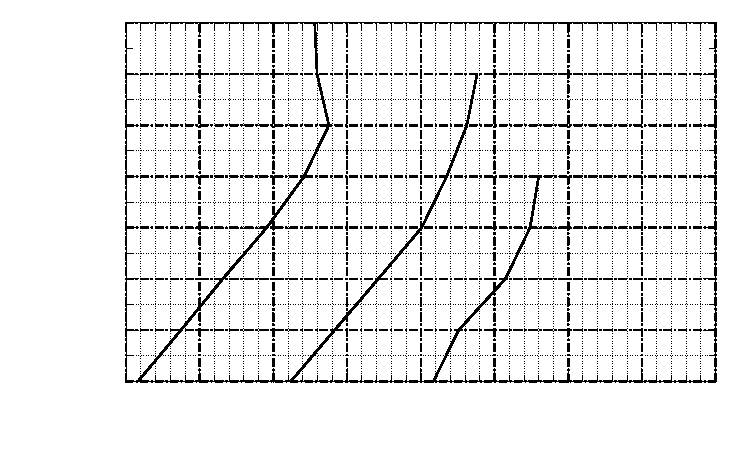
\includegraphics{../graphs/cruise_speed}}%
    \gplfronttext
  \end{picture}%
\endgroup
\end{center}  % for gnuplot epslatex, latex or pslatex mode
\caption{Cruise Speed}
\label{Cruise-speed}
\end{figure}


  % Cruise Speed Chart - Wheel Pants ON
% Cruise Speed Chart - Wheel Pants OFF
\begin{figure}[t]
% \addcontentsline{toc}{section}{Figure \ref{Cruise-speed} Cruise Speed}
\addcontentsline{toc}{section}{CRUISE SPEED - WHEEL PANTS OFF}
\begin{center}
\begin{perfhdr}CRUISE SPEED - WHEEL PANTS OFF\\
\end{perfhdr}

\begin{minipage}{5in}
  \begin{flushleft}
    CONDITIONS:\\
    Wheel Pants OFF, Gear Leg Fairings ON\\
    Standard atmosphere.\\
    Mixture set to best power for 75\% power.\\
    Mixture set to 50\textdegree F lean of peak EGT for 65\% and 55\% power.\\
    Full throttle.\\
    RPM set to obtain desired power, but no higher than 2700 rpm.\\
    \end{flushleft}
\end{minipage}\\
\vspace{5ex}

% GNUPLOT: LaTeX picture with Postscript
\begingroup
  \makeatletter
  \providecommand\color[2][]{%
    \GenericError{(gnuplot) \space\space\space\@spaces}{%
      Package color not loaded in conjunction with
      terminal option `colourtext'%
    }{See the gnuplot documentation for explanation.%
    }{Either use 'blacktext' in gnuplot or load the package
      color.sty in LaTeX.}%
    \renewcommand\color[2][]{}%
  }%
  \providecommand\includegraphics[2][]{%
    \GenericError{(gnuplot) \space\space\space\@spaces}{%
      Package graphicx or graphics not loaded%
    }{See the gnuplot documentation for explanation.%
    }{The gnuplot epslatex terminal needs graphicx.sty or graphics.sty.}%
    \renewcommand\includegraphics[2][]{}%
  }%
  \providecommand\rotatebox[2]{#2}%
  \@ifundefined{ifGPcolor}{%
    \newif\ifGPcolor
    \GPcolorfalse
  }{}%
  \@ifundefined{ifGPblacktext}{%
    \newif\ifGPblacktext
    \GPblacktexttrue
  }{}%
  % define a \g@addto@macro without @ in the name:
  \let\gplgaddtomacro\g@addto@macro
  % define empty templates for all commands taking text:
  \gdef\gplbacktext{}%
  \gdef\gplfronttext{}%
  \makeatother
  \ifGPblacktext
    % no textcolor at all
    \def\colorrgb#1{}%
    \def\colorgray#1{}%
  \else
    % gray or color?
    \ifGPcolor
      \def\colorrgb#1{\color[rgb]{#1}}%
      \def\colorgray#1{\color[gray]{#1}}%
      \expandafter\def\csname LTw\endcsname{\color{white}}%
      \expandafter\def\csname LTb\endcsname{\color{black}}%
      \expandafter\def\csname LTa\endcsname{\color{black}}%
      \expandafter\def\csname LT0\endcsname{\color[rgb]{1,0,0}}%
      \expandafter\def\csname LT1\endcsname{\color[rgb]{0,1,0}}%
      \expandafter\def\csname LT2\endcsname{\color[rgb]{0,0,1}}%
      \expandafter\def\csname LT3\endcsname{\color[rgb]{1,0,1}}%
      \expandafter\def\csname LT4\endcsname{\color[rgb]{0,1,1}}%
      \expandafter\def\csname LT5\endcsname{\color[rgb]{1,1,0}}%
      \expandafter\def\csname LT6\endcsname{\color[rgb]{0,0,0}}%
      \expandafter\def\csname LT7\endcsname{\color[rgb]{1,0.3,0}}%
      \expandafter\def\csname LT8\endcsname{\color[rgb]{0.5,0.5,0.5}}%
    \else
      % gray
      \def\colorrgb#1{\color{black}}%
      \def\colorgray#1{\color[gray]{#1}}%
      \expandafter\def\csname LTw\endcsname{\color{white}}%
      \expandafter\def\csname LTb\endcsname{\color{black}}%
      \expandafter\def\csname LTa\endcsname{\color{black}}%
      \expandafter\def\csname LT0\endcsname{\color{black}}%
      \expandafter\def\csname LT1\endcsname{\color{black}}%
      \expandafter\def\csname LT2\endcsname{\color{black}}%
      \expandafter\def\csname LT3\endcsname{\color{black}}%
      \expandafter\def\csname LT4\endcsname{\color{black}}%
      \expandafter\def\csname LT5\endcsname{\color{black}}%
      \expandafter\def\csname LT6\endcsname{\color{black}}%
      \expandafter\def\csname LT7\endcsname{\color{black}}%
      \expandafter\def\csname LT8\endcsname{\color{black}}%
    \fi
  \fi
  \setlength{\unitlength}{0.0500bp}%
  \begin{picture}(7200.00,5040.00)%
    \gplgaddtomacro\gplbacktext{%
      \csname LTb\endcsname%
      \put(1342,704){\makebox(0,0)[r]{\strut{}0}}%
      \csname LTb\endcsname%
      \put(1342,1286){\makebox(0,0)[r]{\strut{}2,000}}%
      \csname LTb\endcsname%
      \put(1342,1867){\makebox(0,0)[r]{\strut{}4,000}}%
      \csname LTb\endcsname%
      \put(1342,2449){\makebox(0,0)[r]{\strut{}6,000}}%
      \csname LTb\endcsname%
      \put(1342,3030){\makebox(0,0)[r]{\strut{}8,000}}%
      \csname LTb\endcsname%
      \put(1342,3612){\makebox(0,0)[r]{\strut{}10,000}}%
      \csname LTb\endcsname%
      \put(1342,4193){\makebox(0,0)[r]{\strut{}12,000}}%
      \csname LTb\endcsname%
      \put(1342,4775){\makebox(0,0)[r]{\strut{}14,000}}%
      \csname LTb\endcsname%
      \put(1474,484){\makebox(0,0){\strut{} 135}}%
      \csname LTb\endcsname%
      \put(2148,484){\makebox(0,0){\strut{} 140}}%
      \csname LTb\endcsname%
      \put(2823,484){\makebox(0,0){\strut{} 145}}%
      \csname LTb\endcsname%
      \put(3497,484){\makebox(0,0){\strut{} 150}}%
      \csname LTb\endcsname%
      \put(4172,484){\makebox(0,0){\strut{} 155}}%
      \csname LTb\endcsname%
      \put(4846,484){\makebox(0,0){\strut{} 160}}%
      \csname LTb\endcsname%
      \put(5520,484){\makebox(0,0){\strut{} 165}}%
      \csname LTb\endcsname%
      \put(6195,484){\makebox(0,0){\strut{} 170}}%
      \csname LTb\endcsname%
      \put(6869,484){\makebox(0,0){\strut{} 175}}%
      \put(308,2739){\rotatebox{-270}{\makebox(0,0){\strut{}Altitude (ft)}}}%
      \put(4171,154){\makebox(0,0){\strut{}Cruise Speed - Wheel Pants OFF (KTAS)}}%
      \put(5224,1286){\rotatebox{55}{\makebox(0,0)[l]{\strut{}75\% Power}}}%
      \put(4536,1722){\rotatebox{55}{\makebox(0,0)[l]{\strut{}65\% Power}}}%
      \put(3726,2158){\rotatebox{56}{\makebox(0,0)[l]{\strut{}55\% Power}}}%
      \put(1528,4612){\makebox(0,0)[l]{\strut{}From Flight Tests 20 \& 22 Jan 2011}}%
    }%
    \gplgaddtomacro\gplfronttext{%
    }%
    \gplbacktext
    \put(0,0){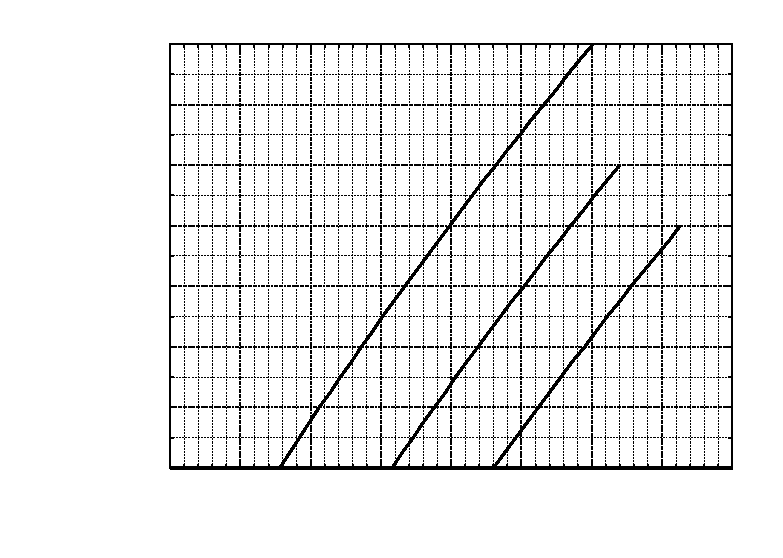
\includegraphics{../graphs/cruise_speed_wheel_pants_off}}%
    \gplfronttext
  \end{picture}%
\endgroup
\end{center}  % for gnuplot epslatex, latex or pslatex mode
\caption{Cruise Speed - Wheel Pants OFF}
\label{Cruise-speed-WP-OFF}
\end{figure}


 % Cruise Speed Chart - Wheel Pants OFF
% Cruise Range Chart - Wheel Pants ON
\begin{figure}[t]
% \addcontentsline{toc}{section}{Figure \ref{Cruise-range} Cruise Range}
\addcontentsline{toc}{section}{CRUISE RANGE}
\begin{center}
\begin{perfhdr}CRUISE RANGE\\
\end{perfhdr}

\begin{minipage}{5in}
  \begin{flushleft}
    CONDITIONS:\\
    Wheel Pants and Gear Leg Fairings ON\\
    43 USG Usable Fuel.\\
    Standard atmosphere.\\
    No wind.\\
    Includes 1.0 USG fuel for start, taxi and takeoff and 8 USG or 45 mn reserve.\\
    Climb at full power and best climb speed as defined on the Maximum Climb Chart\\
    Lean during climb for best power.\\
    Cruise with mixture set to best power for 75\% power.  Mixture set to 50\textdegree F lean of peak EGT for 65\% or less, except mixture set to best power if more than 2600 rpm required with mixture set lean of peak EGT.\\
    Full throttle, but no less than 2100 rpm.\\
    Descend at cruise TAS at 6 nm per 1000 ft.\\
    \end{flushleft}
\end{minipage}\\
\vspace{5ex}
% GNUPLOT: LaTeX picture with Postscript
\begingroup
  \makeatletter
  \providecommand\color[2][]{%
    \GenericError{(gnuplot) \space\space\space\@spaces}{%
      Package color not loaded in conjunction with
      terminal option `colourtext'%
    }{See the gnuplot documentation for explanation.%
    }{Either use 'blacktext' in gnuplot or load the package
      color.sty in LaTeX.}%
    \renewcommand\color[2][]{}%
  }%
  \providecommand\includegraphics[2][]{%
    \GenericError{(gnuplot) \space\space\space\@spaces}{%
      Package graphicx or graphics not loaded%
    }{See the gnuplot documentation for explanation.%
    }{The gnuplot epslatex terminal needs graphicx.sty or graphics.sty.}%
    \renewcommand\includegraphics[2][]{}%
  }%
  \providecommand\rotatebox[2]{#2}%
  \@ifundefined{ifGPcolor}{%
    \newif\ifGPcolor
    \GPcolorfalse
  }{}%
  \@ifundefined{ifGPblacktext}{%
    \newif\ifGPblacktext
    \GPblacktexttrue
  }{}%
  % define a \g@addto@macro without @ in the name:
  \let\gplgaddtomacro\g@addto@macro
  % define empty templates for all commands taking text:
  \gdef\gplbacktext{}%
  \gdef\gplfronttext{}%
  \makeatother
  \ifGPblacktext
    % no textcolor at all
    \def\colorrgb#1{}%
    \def\colorgray#1{}%
  \else
    % gray or color?
    \ifGPcolor
      \def\colorrgb#1{\color[rgb]{#1}}%
      \def\colorgray#1{\color[gray]{#1}}%
      \expandafter\def\csname LTw\endcsname{\color{white}}%
      \expandafter\def\csname LTb\endcsname{\color{black}}%
      \expandafter\def\csname LTa\endcsname{\color{black}}%
      \expandafter\def\csname LT0\endcsname{\color[rgb]{1,0,0}}%
      \expandafter\def\csname LT1\endcsname{\color[rgb]{0,1,0}}%
      \expandafter\def\csname LT2\endcsname{\color[rgb]{0,0,1}}%
      \expandafter\def\csname LT3\endcsname{\color[rgb]{1,0,1}}%
      \expandafter\def\csname LT4\endcsname{\color[rgb]{0,1,1}}%
      \expandafter\def\csname LT5\endcsname{\color[rgb]{1,1,0}}%
      \expandafter\def\csname LT6\endcsname{\color[rgb]{0,0,0}}%
      \expandafter\def\csname LT7\endcsname{\color[rgb]{1,0.3,0}}%
      \expandafter\def\csname LT8\endcsname{\color[rgb]{0.5,0.5,0.5}}%
    \else
      % gray
      \def\colorrgb#1{\color{black}}%
      \def\colorgray#1{\color[gray]{#1}}%
      \expandafter\def\csname LTw\endcsname{\color{white}}%
      \expandafter\def\csname LTb\endcsname{\color{black}}%
      \expandafter\def\csname LTa\endcsname{\color{black}}%
      \expandafter\def\csname LT0\endcsname{\color{black}}%
      \expandafter\def\csname LT1\endcsname{\color{black}}%
      \expandafter\def\csname LT2\endcsname{\color{black}}%
      \expandafter\def\csname LT3\endcsname{\color{black}}%
      \expandafter\def\csname LT4\endcsname{\color{black}}%
      \expandafter\def\csname LT5\endcsname{\color{black}}%
      \expandafter\def\csname LT6\endcsname{\color{black}}%
      \expandafter\def\csname LT7\endcsname{\color{black}}%
      \expandafter\def\csname LT8\endcsname{\color{black}}%
    \fi
  \fi
  \setlength{\unitlength}{0.0500bp}%
  \begin{picture}(7200.00,5040.00)%
    \gplgaddtomacro\gplbacktext{%
      \csname LTb\endcsname%
      \put(1342,704){\makebox(0,0)[r]{\strut{}0}}%
      \csname LTb\endcsname%
      \put(1342,1286){\makebox(0,0)[r]{\strut{}2,000}}%
      \csname LTb\endcsname%
      \put(1342,1867){\makebox(0,0)[r]{\strut{}4,000}}%
      \csname LTb\endcsname%
      \put(1342,2449){\makebox(0,0)[r]{\strut{}6,000}}%
      \csname LTb\endcsname%
      \put(1342,3030){\makebox(0,0)[r]{\strut{}8,000}}%
      \csname LTb\endcsname%
      \put(1342,3612){\makebox(0,0)[r]{\strut{}10,000}}%
      \csname LTb\endcsname%
      \put(1342,4193){\makebox(0,0)[r]{\strut{}12,000}}%
      \csname LTb\endcsname%
      \put(1342,4775){\makebox(0,0)[r]{\strut{}14,000}}%
      \csname LTb\endcsname%
      \put(1474,484){\makebox(0,0){\strut{} 500}}%
      \csname LTb\endcsname%
      \put(2823,484){\makebox(0,0){\strut{} 550}}%
      \csname LTb\endcsname%
      \put(4172,484){\makebox(0,0){\strut{} 600}}%
      \csname LTb\endcsname%
      \put(5520,484){\makebox(0,0){\strut{} 650}}%
      \csname LTb\endcsname%
      \put(6869,484){\makebox(0,0){\strut{} 700}}%
      \put(308,2739){\rotatebox{-270}{\makebox(0,0){\strut{}Altitude (ft)}}}%
      \put(4171,154){\makebox(0,0){\strut{}Cruise Range (NM)}}%
      \put(3227,1373){\rotatebox{77}{\makebox(0,0)[l]{\strut{}75\% Power}}}%
      \put(4576,1727){\rotatebox{76}{\makebox(0,0)[l]{\strut{}65\% Power}}}%
      \put(6060,2158){\rotatebox{76}{\makebox(0,0)[l]{\strut{}55\% Power}}}%
      \put(4172,3874){\makebox(0,0){\strut{}\Large\textcolor{red}{FROM ANALYSIS OF CAFE DATA}\normalsize}}%
      \put(4172,3292){\makebox(0,0){\strut{}\Large\textcolor{red}{PENDING FLIGHT TEST}\normalsize}}%
    }%
    \gplgaddtomacro\gplfronttext{%
    }%
    \gplbacktext
    \put(0,0){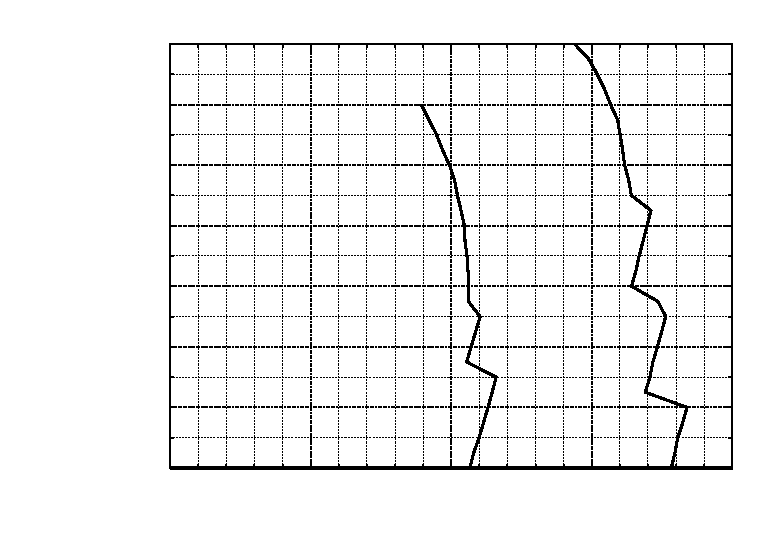
\includegraphics{../graphs/cruise_range}}%
    \gplfronttext
  \end{picture}%
\endgroup
\end{center}  % for gnuplot epslatex, latex or pslatex mode
\caption{Cruise Range}
\label{Cruise-range}
\end{figure}
\clearpage


     % Cruise Range Chart - Wheel Pants ON
% Cruise Range Chart - Wheel Pants OFF
\begin{figure}[t]
% \addcontentsline{toc}{section}{Figure \ref{Cruise-range} Cruise Range}
\addcontentsline{toc}{section}{CRUISE RANGE - WHEEL PANTS OFF}
\begin{center}
\begin{perfhdr}CRUISE RANGE - WHEEL PANTS OFF\\
\end{perfhdr}

\begin{minipage}{5in}
  \begin{flushleft}
    CONDITIONS:\\
    Wheel Pants OFF, Gear Leg Fairings ON\\
    43 USG Usable Fuel.\\
    Standard atmosphere.\\
    No wind.\\
    Includes 1.0 USG fuel for start, taxi and takeoff and 8 USG or 45 mn reserve.\\
    Climb at full power and best climb speed as defined on the Maximum Climb Chart\\
    Lean during climb for best power.\\
    Cruise with mixture set to best power for 75\% power.  \\
    Cruise with mixture set to 50\textdegree F lean of peak EGT for 65\% power or less, except mixture set to best power if more than 2600 rpm required with mixture set lean of peak EGT.\\
    Descend at cruise TAS at 6 nm per 1000 ft.\\
    \end{flushleft}
\end{minipage}\\
\vspace{5ex}
% GNUPLOT: LaTeX picture with Postscript
\begingroup
  \makeatletter
  \providecommand\color[2][]{%
    \GenericError{(gnuplot) \space\space\space\@spaces}{%
      Package color not loaded in conjunction with
      terminal option `colourtext'%
    }{See the gnuplot documentation for explanation.%
    }{Either use 'blacktext' in gnuplot or load the package
      color.sty in LaTeX.}%
    \renewcommand\color[2][]{}%
  }%
  \providecommand\includegraphics[2][]{%
    \GenericError{(gnuplot) \space\space\space\@spaces}{%
      Package graphicx or graphics not loaded%
    }{See the gnuplot documentation for explanation.%
    }{The gnuplot epslatex terminal needs graphicx.sty or graphics.sty.}%
    \renewcommand\includegraphics[2][]{}%
  }%
  \providecommand\rotatebox[2]{#2}%
  \@ifundefined{ifGPcolor}{%
    \newif\ifGPcolor
    \GPcolorfalse
  }{}%
  \@ifundefined{ifGPblacktext}{%
    \newif\ifGPblacktext
    \GPblacktexttrue
  }{}%
  % define a \g@addto@macro without @ in the name:
  \let\gplgaddtomacro\g@addto@macro
  % define empty templates for all commands taking text:
  \gdef\gplbacktext{}%
  \gdef\gplfronttext{}%
  \makeatother
  \ifGPblacktext
    % no textcolor at all
    \def\colorrgb#1{}%
    \def\colorgray#1{}%
  \else
    % gray or color?
    \ifGPcolor
      \def\colorrgb#1{\color[rgb]{#1}}%
      \def\colorgray#1{\color[gray]{#1}}%
      \expandafter\def\csname LTw\endcsname{\color{white}}%
      \expandafter\def\csname LTb\endcsname{\color{black}}%
      \expandafter\def\csname LTa\endcsname{\color{black}}%
      \expandafter\def\csname LT0\endcsname{\color[rgb]{1,0,0}}%
      \expandafter\def\csname LT1\endcsname{\color[rgb]{0,1,0}}%
      \expandafter\def\csname LT2\endcsname{\color[rgb]{0,0,1}}%
      \expandafter\def\csname LT3\endcsname{\color[rgb]{1,0,1}}%
      \expandafter\def\csname LT4\endcsname{\color[rgb]{0,1,1}}%
      \expandafter\def\csname LT5\endcsname{\color[rgb]{1,1,0}}%
      \expandafter\def\csname LT6\endcsname{\color[rgb]{0,0,0}}%
      \expandafter\def\csname LT7\endcsname{\color[rgb]{1,0.3,0}}%
      \expandafter\def\csname LT8\endcsname{\color[rgb]{0.5,0.5,0.5}}%
    \else
      % gray
      \def\colorrgb#1{\color{black}}%
      \def\colorgray#1{\color[gray]{#1}}%
      \expandafter\def\csname LTw\endcsname{\color{white}}%
      \expandafter\def\csname LTb\endcsname{\color{black}}%
      \expandafter\def\csname LTa\endcsname{\color{black}}%
      \expandafter\def\csname LT0\endcsname{\color{black}}%
      \expandafter\def\csname LT1\endcsname{\color{black}}%
      \expandafter\def\csname LT2\endcsname{\color{black}}%
      \expandafter\def\csname LT3\endcsname{\color{black}}%
      \expandafter\def\csname LT4\endcsname{\color{black}}%
      \expandafter\def\csname LT5\endcsname{\color{black}}%
      \expandafter\def\csname LT6\endcsname{\color{black}}%
      \expandafter\def\csname LT7\endcsname{\color{black}}%
      \expandafter\def\csname LT8\endcsname{\color{black}}%
    \fi
  \fi
  \setlength{\unitlength}{0.0500bp}%
  \begin{picture}(7200.00,5040.00)%
    \gplgaddtomacro\gplbacktext{%
      \csname LTb\endcsname%
      \put(1210,704){\makebox(0,0)[r]{\strut{}0}}%
      \csname LTb\endcsname%
      \put(1210,1722){\makebox(0,0)[r]{\strut{}5,000}}%
      \csname LTb\endcsname%
      \put(1210,2740){\makebox(0,0)[r]{\strut{}10,000}}%
      \csname LTb\endcsname%
      \put(1210,3757){\makebox(0,0)[r]{\strut{}15,000}}%
      \csname LTb\endcsname%
      \put(1210,4775){\makebox(0,0)[r]{\strut{}20,000}}%
      \csname LTb\endcsname%
      \put(1342,484){\makebox(0,0){\strut{} 450}}%
      \csname LTb\endcsname%
      \put(1949,484){\makebox(0,0){\strut{} 500}}%
      \csname LTb\endcsname%
      \put(2556,484){\makebox(0,0){\strut{} 550}}%
      \csname LTb\endcsname%
      \put(3162,484){\makebox(0,0){\strut{} 600}}%
      \csname LTb\endcsname%
      \put(3769,484){\makebox(0,0){\strut{} 650}}%
      \csname LTb\endcsname%
      \put(4376,484){\makebox(0,0){\strut{} 700}}%
      \csname LTb\endcsname%
      \put(4983,484){\makebox(0,0){\strut{} 750}}%
      \csname LTb\endcsname%
      \put(5589,484){\makebox(0,0){\strut{} 800}}%
      \csname LTb\endcsname%
      \put(6196,484){\makebox(0,0){\strut{} 850}}%
      \csname LTb\endcsname%
      \put(6803,484){\makebox(0,0){\strut{} 900}}%
      \put(176,2739){\rotatebox{-270}{\makebox(0,0){\strut{}Altitude (ft)}}}%
      \put(4072,154){\makebox(0,0){\strut{}Cruise Range - Wheel Pants OFF (NM)}}%
      \put(1762,1009){\rotatebox{83}{\makebox(0,0)[l]{\strut{}75\% Power}}}%
      \put(3512,1213){\rotatebox{88}{\makebox(0,0)[l]{\strut{}65\% Power}}}%
      \put(4265,1213){\rotatebox{73}{\makebox(0,0)[l]{\strut{}55\% Power}}}%
      \put(5036,1213){\rotatebox{71}{\makebox(0,0)[l]{\strut{}45\% Power}}}%
      \put(5700,1213){\rotatebox{71}{\makebox(0,0)[l]{\strut{}35\% Power}}}%
    }%
    \gplgaddtomacro\gplfronttext{%
    }%
    \gplbacktext
    \put(0,0){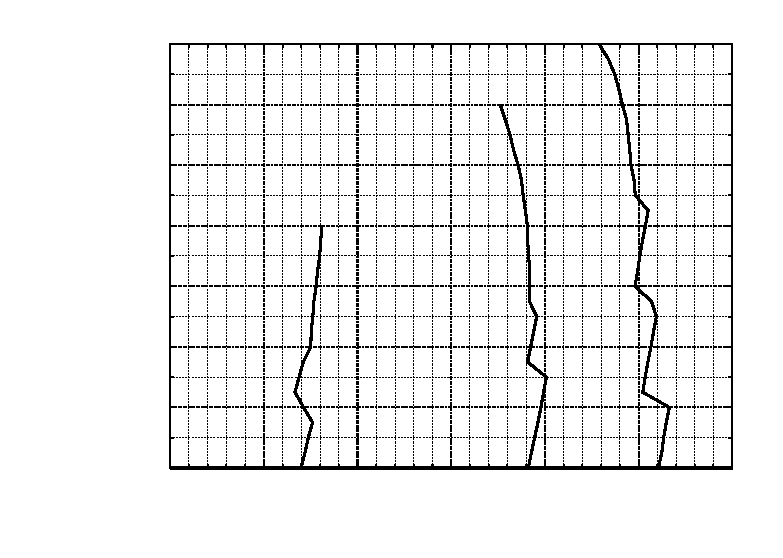
\includegraphics{../graphs/cruise_range_wheel_pants_off}}%
    \gplfronttext
  \end{picture}%
\endgroup
\end{center}  % for gnuplot epslatex, latex or pslatex mode
\caption{Cruise Range - Wheel Pants OFF}
\label{Cruise-range-WP-OFF}
\end{figure}
\clearpage


    % Cruise Range Chart - Wheel Pants OFF
% Landing Distance
\begin{sidewaysfigure}[t]
% \addcontentsline{toc}{section}{Figure \ref{Landing-dist} Landing Distance}
\addcontentsline{toc}{section}{LANDING DISTANCE}
\begin{center}
\begin{perfhdr}LANDING DISTANCE\\
1800 LBS
\end{perfhdr}
\Large
\textcolor{red}{VANS CLAIMED PERF EXPANDED TO OTHER CONDITIONS}\vspace{1ex}\\
\textcolor{red}{TO BE CONFIRMED BY FLIGHT TEST}\normalsize \vspace{5ex}\\

\begin{minipage}{9in}
  \begin{flushleft}
    CONDITIONS:\\
    Full Flaps\\
    Power OFF\\
    Maximum Braking\\
    Paved, Level, Dry Runway\\
    Zero Wind\\

    NOTES:
    \begin{enumerate*}
      \item Short field technique as specified in Section \textcolor{red}{4}.
      \item Decrease distances by 10\% for each 5 knots headwind.  For operations with tailwinds up to 10 knots, increase distances by 10\% for each 2 knots.
      \item For operation on a dry, grass runway, increase distances by 40\% of the ground roll figure.
      \end{enumerate*}
    \end{flushleft}
\end{minipage}\\

\vspace{\perfnoteskip}

\settowidth{\colOne}{WEIGHT}
\settowidth{\colTwo}{SPEED}
\settowidth{\colThree}{PRESS}
\settowidth{\colFour}{GRND}
\settowidth{\colFive}{TOTAL}
\setlength{\rowdrop}{\baselineskip/-1}
\begin{tabular}{|c|c|r|r|r|r|r|r|r|r|r|r|r|}
\hline
\multirow{5}{\colOne}{\centering WEIGHT (LB)}&\multirow{5}{\colTwo}{\centering SPEED AT 50 FT (KIAS)}&
\multirow{5}{\colThree}{\centering PRESS ALT (FT)}&\multicolumn{2}{c|}{0\textdegree C}&
\multicolumn{2}{c|}{10\textdegree C}&\multicolumn{2}{c|}{20\textdegree C}&
\multicolumn{2}{c|}{30\textdegree C}&\multicolumn{2}{c|}{40\textdegree C}\\
\cline{4-13}
&&&\multirow{4}{\colFour}{\centering GRND ROLL (FT)}&\multirow{4}{\colFive}{\centering TOTAL DIST FROM 50 FT}&
\multirow{4}{\colFour}{\centering GRND ROLL (FT)}&\multirow{4}{\colFive}{\centering TOTAL DIST FROM 50 FT}&
\multirow{4}{\colFour}{\centering GRND ROLL (FT)}&\multirow{4}{\colFive}{\centering TOTAL DIST FROM 50 FT}&
\multirow{4}{\colFour}{\centering GRND ROLL (FT)}&\multirow{4}{\colFive}{\centering TOTAL DIST FROM 50 FT}&
\multirow{4}{\colFour}{\centering GRND ROLL (FT)}&\multirow{4}{\colFive}{\centering TOTAL DIST FROM 50 FT}\\
&&&&&&&&&&&&\\ 
&&&&&&&&&&&&\\
&&&&&&&&&&&&\\
\hline
\hline

1800&XX&S.L.&470&TTT&490&TTT&510&TTT&530&TTT&540&TTT\\
\hline
&XX&2,000&510&TTT&530&TTT&550&TTT&570&TTT&580&TTT\\
\hline
&XX&4,000&550&TTT&570&TTT&590&TTT&610&TTT&630&TTT\\
\hline
&XX&6,000&590&TTT&610&TTT&630&TTT&660&TTT&680&TTT\\
\hline
&XX&8,000&640&TTT&660&TTT&680&TTT&710&TTT&730&TTT\\
\hline
&XX&10,000&690&TTT&710&TTT&740&TTT&760&TTT&790&TTT\\
\hline
&XX&12,000&750&TTT&770&TTT&800&TTT&830&TTT&850&TTT\\
\hline
\end{tabular}
\end{center}
\caption{Landing Distance}
\label{Landing-dist}
\end{sidewaysfigure}

                % Landing Distance


\clearpage

\textcolor{red}{To be added once flight test data is available:
\begin{enumerate*}
\item Airspeed Calibration --- Normal Static Source --- Flaps Extended
\item Airspeed Calibration --- Alternate Static Source --- All Flap Positions
\item Altitude Calibration --- Normal Static Source --- Flaps Extended
\item Altitude Calibration --- Alternate Static Source --- All Flap Positions
\item Stall Speeds --- IAS
%\item Range Profile
\item Holding Speed and Fuel Flow
\item Endurance Profile
\end{enumerate*}}
\cleardoublepage

% !iTeXMac(input): POH.tex
\chapter{WEIGHT \& BALANCE}
\vspace{\minitocspacebefore}
\minitoc
%\mtcskip
%\minilof
\cleardoublepage

\section{INTRODUCTION}
This section describes the procedure for establishing the basic empty weight and moment of 
the aircraft.  Sample forms are provided for reference.  Procedures for calculating the 
weight and moment for various operations are also provided.  

\section{AIRCRAFT WEIGHING PROCEDURES}
\begin{enumerate}
  \item Preparation:
    \begin{enumerate}
      \item Inflate tires to recommended operating pressures.
      \item Drain all fuel from the fuel tanks.
      \item Ensure the oil sump is filled to 8 US quarts.
      \item Remove all items from forward and aft baggage area and cockpit pockets.
      \item Raise flaps to the fully retracted position.
      \item Place all control surfaces in the neutral position.
    \end{enumerate}
  \item Levelling:
    \begin{enumerate}
      \item Place scales under each wheel (minimum capacity, 600 lb for main gear, 200 lb for tail wheel).
      \item Place shims under main wheels as necessary to level aircraft laterally.
      \item Raise tail wheel with support until a level on the canopy rail indicates level.
      \suspend{enumerate}
  
   \resume{enumerate}
   \item Close and lock the canopy.
    \end{enumerate}
  \item Weighing:
  \label{weighing}
    \begin{enumerate}
      \item With the aircraft level, record weight shown on each scale.  Deduct the tare weight from each reading.
    \end{enumerate}
  \item Measuring:
  \label{measuring}
    \begin{enumerate}
      \item Drop a plumb bob from the wing leading edge behind each main gear and mark the floor.  Measure 70 inches
forward of this line and mark the floor for the location of the datum.
      \item Measure the horizontal distance from the datum (parallel to the aircraft centre line) to each main wheel
centre.
      \item Measure the horizontal distance (along the aircraft centre line) from the datum to the centre
of the tail wheel axle.
    \end{enumerate}
  \item Using weights from item \ref{weighing} and measurements from item \ref{measuring}, the aircraft weight and CG
can be determined.\label{calc-wb}
  \item Basic Empty Weight may be determined by completing Figure \ref{WB-SampleChart}.
  \end{enumerate}

\begin{figure}
\addcontentsline{toc}{section}{Figure \ref{WB-SampleChart} Sample Aircraft Weighing Record}
\begin{center}
\begin{perfhdr}SAMPLE AIRCRAFT WEIGHING RECORD
  \end{perfhdr}
\settowidth{\colOne}{Right Wheel}
\settowidth{\colTwo}{Distance}
\settowidth{\colThree}{Reading}
\settowidth{\colFour}{Tare}
\settowidth{\colFive}{Weight}
\settowidth{\colSix}{(Moment/1000)}

\begin{overpic}[scale=.7]{../Diagrams/WB-SideView}
  \put(42.3,18.1){CG}
  \put(6,16){70"}
  \put(12,7){DL \& DR}
  \put(70,3){DT}
  \put(19,30.5){X}
  \put(-5,15){\rotatebox{90}{DATUM}}
  % cgspot is not working with dvipdfmx
  % \put(39.2,17.7){
\includegraphics[scale=0.08]{../Diagrams/cgspot}}
  \put(39.2,17.7){
\includegraphics[scale=0.08]{../Diagrams/cgspot2}}
  \end{overpic}  

\vspace{0.2in}
\begin{tabular}{|l|c|c|c|c|c|}
\hline
&\multirow{4}{\colTwo}{\centering Arm (in)}&\multirow{4}{\colThree}{\centering Scale
Reading (lb)}&\multirow{4}{\colFour}{\centering Tare (lb)}&\multirow{4}{\colFive}{\centering Net Weight (lb)}&

\multicolumn{1}{c|}{Moment/1000}\\
\multicolumn{1}{|c|}{Scale}&&&&&\multicolumn{1}{c|}{(Arm x Net}\\
\multicolumn{1}{|c|}{Position}&&&&&\multicolumn{1}{c|}{Weight/1000)}\\
&&&&&\multicolumn{1}{c|}{(lb-in)}\\
\hline
\hline
Left Wheel&\multicolumn{1}{l|}{DL=\hspace*{.7in}}&&&\multicolumn{1}{l|}{L=}&\\
\hline
Right Wheel&\multicolumn{1}{l|}{DR=}&&&\multicolumn{1}{l|}{R=}&\\
\hline
Tail Wheel&\multicolumn{1}{l|}{DT=}&&&\multicolumn{1}{l|}{T=}&\\
%\whline
\hline
\hline
\multicolumn{4}{|l|}{Sum of Net Weights and Moments}&W=\hspace*{.7in}&M=\hspace*{1in}\\
\hline
\end{tabular}\\
\vspace{.2in}
\begin{tabular}{lcr}
$\mathrm{CG(X)=ARM=\frac{M}{W}}$&\hspace{1in}&CG(X)=\makebox[.75in]{\hrulefill} in
\end{tabular}
\vspace{0.2in}
\settowidth{\colOne}{Aircraft Weight (From Item \ref{calc-wb}, page \pageref{calc-wb})}
\settowidth{\colTwo}{Weight}
\settowidth{\colThree}{CG Arm}
\begin{tabular}{|l|c|c|c|}
\hline
\multirow{2}{\colOne}{\centering Item}&\multirow{2}{\colTwo}{\centering Weight (lb)}&\multirow{2}{\colThree}{\centering CG Arm (in)}&Moment/1000\\
&&&(lb-in)\\
\hline
\hline
Aircraft Weight (From Item \ref{calc-wb}, page \pageref{calc-wb})&&&\\
% \hline
% Add Oil: (\textcolor{red}{XX} Qts at 7.5 lbs/Gal)&&\textcolor{red}{XX} in&\\
\hline
Add Unusable Fuel: (0.2 USG at 6.01 lbs/Gal)&&\textcolor{red}{XX} in&\\
\hline
Equipment Changes&&&\\
%\whline
\hline
\hline
Aircraft Basic Empty Weight&&&\\
\hline
\end{tabular}
\end{center}

\caption{Sample Aircraft Weighing Record}
\label{WB-SampleChart}
\end{figure}

\begin{sidewaysfigure}
\addcontentsline{toc}{section}{Figure \ref{Sample-WB-Record} Sample Weight and Balance Record}

\begin{center}
\begin{perfhdr}SAMPLE WEIGHT AND BALANCE RECORD 
  \end{perfhdr}
(Continuous History of Changes in Structure or Equipment Affecting Weight and Balance)\\
\vspace{.1in}

\settowidth{\colOne}{DATE}

\begin{tabular}{|c|c|c|c||c|c|c||c|c|c||c|c|}
\hline
\multicolumn{4}{|l||}{AIRCRAFT MODEL: RV-8}&\multicolumn{5}{l|}{SERIAL NUMBER: 80427}&\multicolumn{3}{l|}{PAGE NUMBER:}\\
\hline
\multirow{4}{\colOne}{\centering DATE}&\multicolumn{2}{c|}{ITEM NO.}&&
\multicolumn{6}{c||}{WEIGHT CHANGE}&\multicolumn{2}{c|}{RUNNING BASIC}\\
\cline{2-3}
\cline{5-10}
&&&DESCRIPTION&\multicolumn{3}{c||}{ADDED (+)}&\multicolumn{3}{c||}{REMOVED (-)}&\multicolumn{2}{c|}{EMPTY WEIGHT}\\
\cline{5-12}
&In&Out&OF ARTICLE OR MODIFICATION&Wt.&Arm&Moment&Wt.&Arm&Moment&Wt.&Moment\\
&&&&(lb.)&(In.)&/1000&(lb.)&(In.)&/1000&(lb.)&/1000\\
\hline
\hline
&&&&&&&&&&& \\
\hline
&&&&&&&&&&& \\
\hline
&&&&&&&&&&& \\
\hline
&&&&&&&&&&& \\
\hline
&&&&&&&&&&& \\
\hline
&&&&&&&&&&& \\
\hline
&&&&&&&&&&& \\
\hline
&&&&&&&&&&& \\
\hline
&&&&&&&&&&& \\
\hline
&&&&&&&&&&& \\
\hline
&&&&&&&&&&& \\
\hline
&&&&&&&&&&& \\
\hline
&&&&&&&&&&& \\
\hline
&&&&&&&&&&& \\
\hline
&&&&&&&&&&& \\
\hline
&&&&&&&&&&& \\
\hline
&&&&&&&&&&& \\
\hline
&&&&&&&&&&& \\
\hline
&&&&&&&&&&& \\
\hline
\end{tabular}
\caption{Sample Weight and Balance Record}
\label{Sample-WB-Record}
\end{center}
\end{sidewaysfigure}

\clearpage

\section{WEIGHT AND BALANCE}

The following information will explain how to load and operate the aircraft so that the weight and centre of gravity remain with the prescribed limits.  The weight and balance is determined as follows:

\begin{enumerate}
\item Take the basic empty weight and moment from the appropriate weight and balance records and enter them in the column ``YOUR AIRCRAFT'' on the Sample Loading Problem.
\begin{Note}
In addition to the basic empty weight and moment noted on the these records, the CG arm (fuselage station) is also shown, but need not be used on the Sample Loading Problem.  The moment which is shown must be divided by 1000 and this value used as the moment/1000 on the loading problem.
\end{Note}
\item Use the Loading Graph to determine the moment/1000 for each additional item to be carried, then list these on the loading problem.
\begin{Note}
Loading Graph information for the forward and aft baggage areas and hat shelf is based on the
 load being located in the centre of these areas, as shown on the Loading Arrangements 
 Diagram.  For loadings which differ from these, the Sample Loading Problem lists the range of fuselage 
 stations for these areas.  The actual fuselage station of the load in question must be entered on the Sample Loading Problem, and the moment must be calculated.
\end{Note}

\item Total the weights and moments/1000 and plot the values for zero fuel on the Centre of Gravity Moment Envelope to determine whether the point falls within the envelope.
\item Add the fuel weight and moment/1000 and plot the values for the loaded aircraft on the Centre of Gravity Moment Envelope to determine whether the point falls within the envelope.
\end{enumerate}

\section{BAGGAGE TIE-DOWNS}
There are four removable tie down rings on the floor of the aft baggage compartment.

\begin{figure}
\addcontentsline{toc}{section}{Figure \ref{Baggage-Compartments} Baggage Compartments}

\begin{overpic}{../Diagrams/Loading-Arrangements}
  \put(32,38){Front Baggage Compartment}
  \put(80,38){Rear Baggage Compartment}
  % The following commands work with the pspicture package
  % \put(31,38){\Vector(0,7)}
  % \put(31,37){\Vector(0,-12)}
  % \put(30.5,37.5){\Vector(-10,-5)}
  % \put(79,38){\Vector(0,11)}
  % \put(79,37){\Vector(0,-10)}

  % The following commands work with the pict2e package
  \put(31,38){\vector(0,1){7}}
  \put(31,37){\vector(0,-1){12}}
  \put(30.5,37.5){\vector(-10,-5){10}}
  \put(79,38){\vector(0,1){11}}
  \put(79,37){\vector(0,-1){10}}
  \end{overpic}
\caption{Baggage Compartments}
\label{Baggage-Compartments}
\end{figure}

\begin{figure}
\addcontentsline{toc}{section}{Figure \ref{Loading-Form} Loading Form}

\begin{center}
  \settowidth{\colOne}{AFT BAGGAGE FLOOR}
  \begin{tabular}{|r|r|r|r|}
    \hline
    \multirow{2}{\colOne}{\centering\bfseries{ITEM}}&\multicolumn{1}{|c|}{\bfseries{WEIGHT}}&\multicolumn{1}{c|}{\bfseries{ARM}}& \multicolumn{1}{c|}{\bfseries{MOMENT/1000}}\\
    &\multicolumn{1}{|c|}{\bfseries{(LB)}}&\multicolumn{1}{c|}{\bfseries{(IN)}}& \multicolumn{1}{c|}{\bfseries{(LB-IN)}}\\
    \hline\hline
    EMPTY AIRCRAFT&&&\\
    \hline
    FWD BAGGAGE&&58.51&\\
    \hline
    FUEL (258.4 LB MAX)&&80.00&\\
    \hline
    PILOT&&91.78&\\
    \hline
    PASSENGER&&119.12&\\
    \hline
    AFT BAGGAGE FLOOR&&138.00&\\
    \hline
    AFT BAGGAGE SHELF&&152.91&\\
    \hline
    OTHER&&&\\
    \hline \hline
   TOTAL&&\multicolumn{1}{c|}{- -}&\\
    \hline
    \multicolumn{1}{r|}{CG}&\\
    \cline{2-2}
    \end{tabular}

  \caption{Loading Form}
  \label{Loading-Form}
  \end{center}
  \end{figure}

\begin{figure}
\addcontentsline{toc}{section}{Figure \ref{Sample-Loading-Problem} Sample Loading Problem}

\begin{center}
  \settowidth{\colOne}{AFT BAGGAGE FLOOR}
  \begin{tabular}{|r|r|r|r|}
    \hline
    \multirow{2}{\colOne}{\centering\bfseries{ITEM}}&\multicolumn{1}{|c|}{\bfseries{WEIGHT}}&\multicolumn{1}{c|}{\bfseries{ARM}}& \multicolumn{1}{c|}{\bfseries{MOMENT/1000}}\\
    &\multicolumn{1}{|c|}{\bfseries{(LB)}}&\multicolumn{1}{c|}{\bfseries{(IN)}}& \multicolumn{1}{c|}{\bfseries{(LB-IN)}}\\
    \hline\hline
    EMPTY AIRCRAFT&1,069&76.26&81.52\\
    \hline
    FWD BAGGAGE&25&58.51&1.46\\
    \hline
    FUEL (258.4 LB MAX)&232&80.00&18.56\\
    \hline
    PILOT&170&91.78&15.60\\
    \hline
    PASSENGER&230&119.12&27.39\\
    \hline
    AFT BAGGAGE FLOOR&50&138.00&6.90\\
    \hline
    AFT BAGGAGE SHELF&24&152.91&3.66\\
    \hline
    OTHER&&&\\
    \hline \hline
   TOTAL&1,800&\multicolumn{1}{c|}{- -}&155.11\\
    \hline
    \multicolumn{1}{r|}{CG}&86.18&\multicolumn{2}{l}{CG WITHIN LIMITS}\\
    \cline{2-2}
    \end{tabular}

  \caption{Sample Loading Problem}
  \label{Sample-Loading-Problem}
  \end{center}
  \end{figure}

\begin{sidewaysfigure}
\addcontentsline{toc}{section}{Figure \ref{Loading-Graph} Loading Graph}

\begin{center}
  % GNUPLOT: LaTeX picture with Postscript
\begingroup
  \makeatletter
  \providecommand\color[2][]{%
    \GenericError{(gnuplot) \space\space\space\@spaces}{%
      Package color not loaded in conjunction with
      terminal option `colourtext'%
    }{See the gnuplot documentation for explanation.%
    }{Either use 'blacktext' in gnuplot or load the package
      color.sty in LaTeX.}%
    \renewcommand\color[2][]{}%
  }%
  \providecommand\includegraphics[2][]{%
    \GenericError{(gnuplot) \space\space\space\@spaces}{%
      Package graphicx or graphics not loaded%
    }{See the gnuplot documentation for explanation.%
    }{The gnuplot epslatex terminal needs graphicx.sty or graphics.sty.}%
    \renewcommand\includegraphics[2][]{}%
  }%
  \providecommand\rotatebox[2]{#2}%
  \@ifundefined{ifGPcolor}{%
    \newif\ifGPcolor
    \GPcolorfalse
  }{}%
  \@ifundefined{ifGPblacktext}{%
    \newif\ifGPblacktext
    \GPblacktexttrue
  }{}%
  % define a \g@addto@macro without @ in the name:
  \let\gplgaddtomacro\g@addto@macro
  % define empty templates for all commands taking text:
  \gdef\gplbacktext{}%
  \gdef\gplfronttext{}%
  \makeatother
  \ifGPblacktext
    % no textcolor at all
    \def\colorrgb#1{}%
    \def\colorgray#1{}%
  \else
    % gray or color?
    \ifGPcolor
      \def\colorrgb#1{\color[rgb]{#1}}%
      \def\colorgray#1{\color[gray]{#1}}%
      \expandafter\def\csname LTw\endcsname{\color{white}}%
      \expandafter\def\csname LTb\endcsname{\color{black}}%
      \expandafter\def\csname LTa\endcsname{\color{black}}%
      \expandafter\def\csname LT0\endcsname{\color[rgb]{1,0,0}}%
      \expandafter\def\csname LT1\endcsname{\color[rgb]{0,1,0}}%
      \expandafter\def\csname LT2\endcsname{\color[rgb]{0,0,1}}%
      \expandafter\def\csname LT3\endcsname{\color[rgb]{1,0,1}}%
      \expandafter\def\csname LT4\endcsname{\color[rgb]{0,1,1}}%
      \expandafter\def\csname LT5\endcsname{\color[rgb]{1,1,0}}%
      \expandafter\def\csname LT6\endcsname{\color[rgb]{0,0,0}}%
      \expandafter\def\csname LT7\endcsname{\color[rgb]{1,0.3,0}}%
      \expandafter\def\csname LT8\endcsname{\color[rgb]{0.5,0.5,0.5}}%
    \else
      % gray
      \def\colorrgb#1{\color{black}}%
      \def\colorgray#1{\color[gray]{#1}}%
      \expandafter\def\csname LTw\endcsname{\color{white}}%
      \expandafter\def\csname LTb\endcsname{\color{black}}%
      \expandafter\def\csname LTa\endcsname{\color{black}}%
      \expandafter\def\csname LT0\endcsname{\color{black}}%
      \expandafter\def\csname LT1\endcsname{\color{black}}%
      \expandafter\def\csname LT2\endcsname{\color{black}}%
      \expandafter\def\csname LT3\endcsname{\color{black}}%
      \expandafter\def\csname LT4\endcsname{\color{black}}%
      \expandafter\def\csname LT5\endcsname{\color{black}}%
      \expandafter\def\csname LT6\endcsname{\color{black}}%
      \expandafter\def\csname LT7\endcsname{\color{black}}%
      \expandafter\def\csname LT8\endcsname{\color{black}}%
    \fi
  \fi
  \setlength{\unitlength}{0.0500bp}%
  \begin{picture}(12960.00,10080.00)%
    \gplgaddtomacro\gplbacktext{%
      \csname LTb\endcsname%
      \put(1078,704){\makebox(0,0)[r]{\strut{} 0}}%
      \csname LTb\endcsname%
      \put(1078,2156){\makebox(0,0)[r]{\strut{} 50}}%
      \csname LTb\endcsname%
      \put(1078,3609){\makebox(0,0)[r]{\strut{} 100}}%
      \csname LTb\endcsname%
      \put(1078,5061){\makebox(0,0)[r]{\strut{} 150}}%
      \csname LTb\endcsname%
      \put(1078,6513){\makebox(0,0)[r]{\strut{} 200}}%
      \csname LTb\endcsname%
      \put(1078,7966){\makebox(0,0)[r]{\strut{} 250}}%
      \csname LTb\endcsname%
      \put(1078,9418){\makebox(0,0)[r]{\strut{} 300}}%
      \csname LTb\endcsname%
      \put(1210,484){\makebox(0,0){\strut{} 0}}%
      \csname LTb\endcsname%
      \put(2944,484){\makebox(0,0){\strut{} 5}}%
      \csname LTb\endcsname%
      \put(4679,484){\makebox(0,0){\strut{} 10}}%
      \csname LTb\endcsname%
      \put(6413,484){\makebox(0,0){\strut{} 15}}%
      \csname LTb\endcsname%
      \put(8147,484){\makebox(0,0){\strut{} 20}}%
      \csname LTb\endcsname%
      \put(9882,484){\makebox(0,0){\strut{} 25}}%
      \csname LTb\endcsname%
      \put(11616,484){\makebox(0,0){\strut{} 30}}%
      \put(11748,704){\makebox(0,0)[l]{\strut{} 0}}%
      \put(11748,2156){\makebox(0,0)[l]{\strut{} 50}}%
      \put(11748,3609){\makebox(0,0)[l]{\strut{} 100}}%
      \put(11748,5061){\makebox(0,0)[l]{\strut{} 150}}%
      \put(11748,6513){\makebox(0,0)[l]{\strut{} 200}}%
      \put(11748,7966){\makebox(0,0)[l]{\strut{} 250}}%
      \put(11748,9418){\makebox(0,0)[l]{\strut{} 300}}%
      \put(1210,9638){\makebox(0,0){\strut{} 0}}%
      \put(2944,9638){\makebox(0,0){\strut{} 5}}%
      \put(4679,9638){\makebox(0,0){\strut{} 10}}%
      \put(6413,9638){\makebox(0,0){\strut{} 15}}%
      \put(8147,9638){\makebox(0,0){\strut{} 20}}%
      \put(9882,9638){\makebox(0,0){\strut{} 25}}%
      \put(11616,9638){\makebox(0,0){\strut{} 30}}%
      \put(308,5061){\rotatebox{-270}{\makebox(0,0){\strut{}Load Weight (lb)}}}%
      \put(12517,5061){\rotatebox{-270}{\makebox(0,0){\strut{}Load Weight (lb)}}}%
      \put(6413,154){\makebox(0,0){\strut{}Load Moment/1000 (pound-inches)}}%
      \put(6413,9967){\makebox(0,0){\strut{}Load Moment/1000 (pound-inches)}}%
      \put(6240,6223){\rotatebox{39}{\makebox(0,0)[l]{\strut{}\Large Fuel\normalsize}}}%
      \put(7558,6223){\rotatebox{36}{\makebox(0,0)[l]{\strut{}\Large Pilot\normalsize}}}%
      \put(9465,6223){\rotatebox{29}{\makebox(0,0)[l]{\strut{}\Large Passenger\normalsize}}}%
      \put(5893,2447){\makebox(0,0)[l]{\strut{}\Large Rear Baggage Compartment Floor\normalsize}}%
      \put(1730,3028){\rotatebox{90}{\makebox(0,0)[l]{\strut{}\Large Front Baggage Compartment\normalsize}}}%
      \put(3638,994){\makebox(0,0)[l]{\strut{}\Large Rear Baggage Compartment Shelf\normalsize}}%
    }%
    \gplgaddtomacro\gplfronttext{%
    }%
    \gplbacktext
    \put(0,0){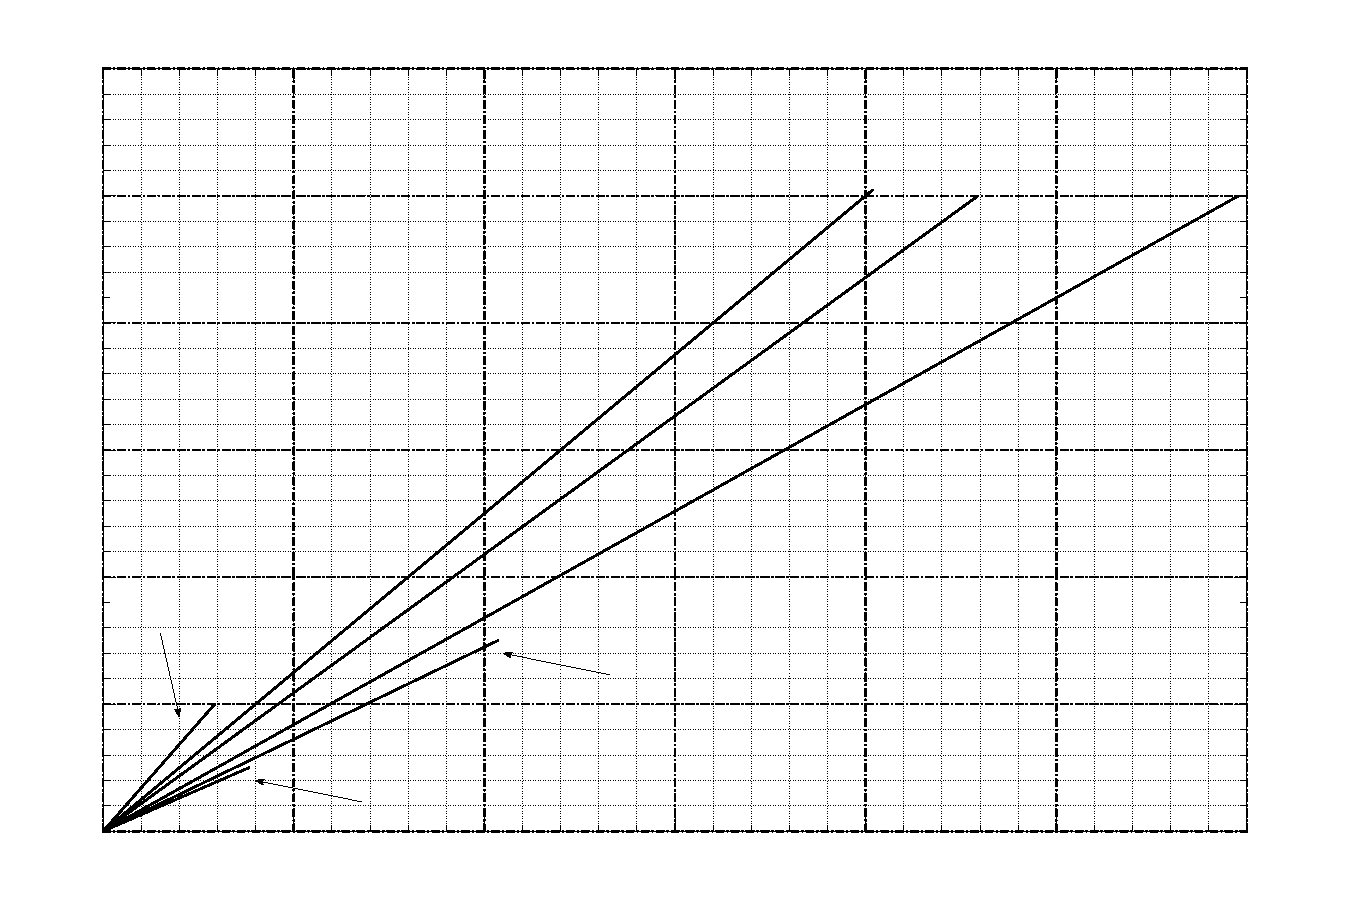
\includegraphics{../graphs/wb-loading-graph}}%
    \gplfronttext
  \end{picture}%
\endgroup

  \end{center}

\caption{Loading Graph}
\label{Loading-Graph}
\end{sidewaysfigure}

\begin{figure}
\addcontentsline{toc}{section}{Figure \ref{CG-Moment} CG Moment Envelope}
\begin{center}
  \ifthenelse{\theMTOW > 1800}{% GNUPLOT: LaTeX picture with Postscript
\begingroup
  \makeatletter
  \providecommand\color[2][]{%
    \GenericError{(gnuplot) \space\space\space\@spaces}{%
      Package color not loaded in conjunction with
      terminal option `colourtext'%
    }{See the gnuplot documentation for explanation.%
    }{Either use 'blacktext' in gnuplot or load the package
      color.sty in LaTeX.}%
    \renewcommand\color[2][]{}%
  }%
  \providecommand\includegraphics[2][]{%
    \GenericError{(gnuplot) \space\space\space\@spaces}{%
      Package graphicx or graphics not loaded%
    }{See the gnuplot documentation for explanation.%
    }{The gnuplot epslatex terminal needs graphicx.sty or graphics.sty.}%
    \renewcommand\includegraphics[2][]{}%
  }%
  \providecommand\rotatebox[2]{#2}%
  \@ifundefined{ifGPcolor}{%
    \newif\ifGPcolor
    \GPcolorfalse
  }{}%
  \@ifundefined{ifGPblacktext}{%
    \newif\ifGPblacktext
    \GPblacktexttrue
  }{}%
  % define a \g@addto@macro without @ in the name:
  \let\gplgaddtomacro\g@addto@macro
  % define empty templates for all commands taking text:
  \gdef\gplbacktext{}%
  \gdef\gplfronttext{}%
  \makeatother
  \ifGPblacktext
    % no textcolor at all
    \def\colorrgb#1{}%
    \def\colorgray#1{}%
  \else
    % gray or color?
    \ifGPcolor
      \def\colorrgb#1{\color[rgb]{#1}}%
      \def\colorgray#1{\color[gray]{#1}}%
      \expandafter\def\csname LTw\endcsname{\color{white}}%
      \expandafter\def\csname LTb\endcsname{\color{black}}%
      \expandafter\def\csname LTa\endcsname{\color{black}}%
      \expandafter\def\csname LT0\endcsname{\color[rgb]{1,0,0}}%
      \expandafter\def\csname LT1\endcsname{\color[rgb]{0,1,0}}%
      \expandafter\def\csname LT2\endcsname{\color[rgb]{0,0,1}}%
      \expandafter\def\csname LT3\endcsname{\color[rgb]{1,0,1}}%
      \expandafter\def\csname LT4\endcsname{\color[rgb]{0,1,1}}%
      \expandafter\def\csname LT5\endcsname{\color[rgb]{1,1,0}}%
      \expandafter\def\csname LT6\endcsname{\color[rgb]{0,0,0}}%
      \expandafter\def\csname LT7\endcsname{\color[rgb]{1,0.3,0}}%
      \expandafter\def\csname LT8\endcsname{\color[rgb]{0.5,0.5,0.5}}%
    \else
      % gray
      \def\colorrgb#1{\color{black}}%
      \def\colorgray#1{\color[gray]{#1}}%
      \expandafter\def\csname LTw\endcsname{\color{white}}%
      \expandafter\def\csname LTb\endcsname{\color{black}}%
      \expandafter\def\csname LTa\endcsname{\color{black}}%
      \expandafter\def\csname LT0\endcsname{\color{black}}%
      \expandafter\def\csname LT1\endcsname{\color{black}}%
      \expandafter\def\csname LT2\endcsname{\color{black}}%
      \expandafter\def\csname LT3\endcsname{\color{black}}%
      \expandafter\def\csname LT4\endcsname{\color{black}}%
      \expandafter\def\csname LT5\endcsname{\color{black}}%
      \expandafter\def\csname LT6\endcsname{\color{black}}%
      \expandafter\def\csname LT7\endcsname{\color{black}}%
      \expandafter\def\csname LT8\endcsname{\color{black}}%
    \fi
  \fi
  \setlength{\unitlength}{0.0500bp}%
  \begin{picture}(9360.00,10080.00)%
    \gplgaddtomacro\gplbacktext{%
      \csname LTb\endcsname%
      \put(1210,704){\makebox(0,0)[r]{\strut{} 1100}}%
      \csname LTb\endcsname%
      \put(1210,1672){\makebox(0,0)[r]{\strut{} 1200}}%
      \csname LTb\endcsname%
      \put(1210,2640){\makebox(0,0)[r]{\strut{} 1300}}%
      \csname LTb\endcsname%
      \put(1210,3609){\makebox(0,0)[r]{\strut{} 1400}}%
      \csname LTb\endcsname%
      \put(1210,4577){\makebox(0,0)[r]{\strut{} 1500}}%
      \csname LTb\endcsname%
      \put(1210,5545){\makebox(0,0)[r]{\strut{} 1600}}%
      \csname LTb\endcsname%
      \put(1210,6513){\makebox(0,0)[r]{\strut{} 1700}}%
      \csname LTb\endcsname%
      \put(1210,7482){\makebox(0,0)[r]{\strut{} 1800}}%
      \csname LTb\endcsname%
      \put(1210,8450){\makebox(0,0)[r]{\strut{} 1900}}%
      \csname LTb\endcsname%
      \put(1210,9418){\makebox(0,0)[r]{\strut{} 2000}}%
      \csname LTb\endcsname%
      \put(1342,484){\makebox(0,0){\strut{} 80}}%
      \csname LTb\endcsname%
      \put(2069,484){\makebox(0,0){\strut{} 90}}%
      \csname LTb\endcsname%
      \put(2796,484){\makebox(0,0){\strut{} 100}}%
      \csname LTb\endcsname%
      \put(3523,484){\makebox(0,0){\strut{} 110}}%
      \csname LTb\endcsname%
      \put(4250,484){\makebox(0,0){\strut{} 120}}%
      \csname LTb\endcsname%
      \put(4976,484){\makebox(0,0){\strut{} 130}}%
      \csname LTb\endcsname%
      \put(5703,484){\makebox(0,0){\strut{} 140}}%
      \csname LTb\endcsname%
      \put(6430,484){\makebox(0,0){\strut{} 150}}%
      \csname LTb\endcsname%
      \put(7157,484){\makebox(0,0){\strut{} 160}}%
      \csname LTb\endcsname%
      \put(7884,484){\makebox(0,0){\strut{} 170}}%
      \put(8016,704){\makebox(0,0)[l]{\strut{} 1100}}%
      \put(8016,1672){\makebox(0,0)[l]{\strut{} 1200}}%
      \put(8016,2640){\makebox(0,0)[l]{\strut{} 1300}}%
      \put(8016,3609){\makebox(0,0)[l]{\strut{} 1400}}%
      \put(8016,4577){\makebox(0,0)[l]{\strut{} 1500}}%
      \put(8016,5545){\makebox(0,0)[l]{\strut{} 1600}}%
      \put(8016,6513){\makebox(0,0)[l]{\strut{} 1700}}%
      \put(8016,7482){\makebox(0,0)[l]{\strut{} 1800}}%
      \put(8016,8450){\makebox(0,0)[l]{\strut{} 1900}}%
      \put(8016,9418){\makebox(0,0)[l]{\strut{} 2000}}%
      \put(1342,9638){\makebox(0,0){\strut{} 80}}%
      \put(2069,9638){\makebox(0,0){\strut{} 90}}%
      \put(2796,9638){\makebox(0,0){\strut{} 100}}%
      \put(3523,9638){\makebox(0,0){\strut{} 110}}%
      \put(4250,9638){\makebox(0,0){\strut{} 120}}%
      \put(4976,9638){\makebox(0,0){\strut{} 130}}%
      \put(5703,9638){\makebox(0,0){\strut{} 140}}%
      \put(6430,9638){\makebox(0,0){\strut{} 150}}%
      \put(7157,9638){\makebox(0,0){\strut{} 160}}%
      \put(7884,9638){\makebox(0,0){\strut{} 170}}%
      \put(308,5061){\rotatebox{-270}{\makebox(0,0){\strut{}Weight (lb)}}}%
      \put(8917,5061){\rotatebox{-270}{\makebox(0,0){\strut{}Weight (lb)}}}%
      \put(4613,154){\makebox(0,0){\strut{}Moment/1000 (pound-inches)}}%
      \put(4613,9967){\makebox(0,0){\strut{}Moment/1000 (pound-inches)}}%
    }%
    \gplgaddtomacro\gplfronttext{%
      \put(3523,8934){\makebox(0,0){\strut{}\Large \bfseries \sffamily Normal Weight/Moment Envelope}}%
      \put(3159,7240){\makebox(0,0){\strut{}\Large \bfseries \sffamily Restricted Aerobatic}}%
      \put(3159,6755){\makebox(0,0){\strut{}\Large \bfseries \sffamily Weight/Moment Envelope}}%
      \put(5340,1188){\makebox(0,0){\strut{}\Large \bfseries \sffamily Aerobatic Weight/Moment Envelope}}%
    }%
    \gplbacktext
    \put(0,0){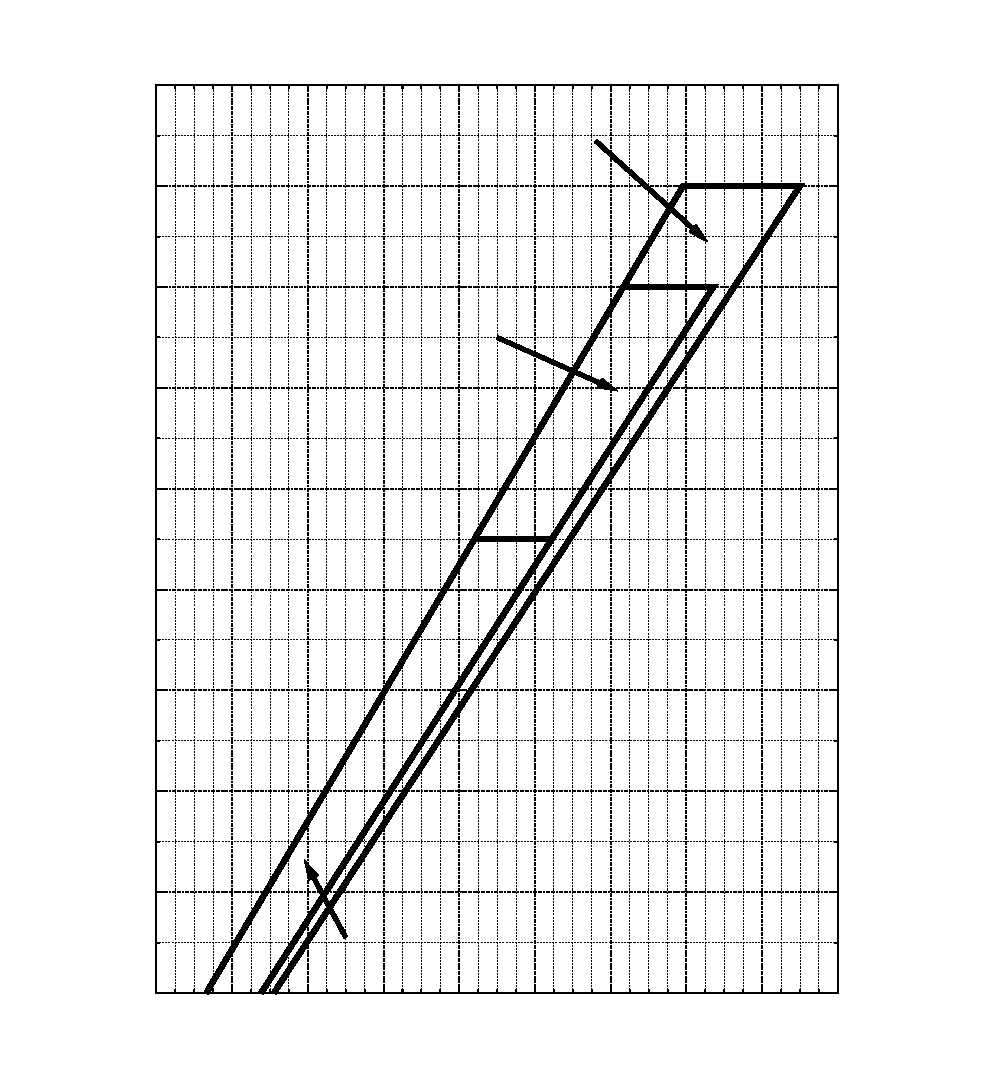
\includegraphics{../graphs/wb-moment-chart1900}}%
    \gplfronttext
  \end{picture}%
\endgroup
}{% GNUPLOT: LaTeX picture with Postscript
\begingroup
  \makeatletter
  \providecommand\color[2][]{%
    \GenericError{(gnuplot) \space\space\space\@spaces}{%
      Package color not loaded in conjunction with
      terminal option `colourtext'%
    }{See the gnuplot documentation for explanation.%
    }{Either use 'blacktext' in gnuplot or load the package
      color.sty in LaTeX.}%
    \renewcommand\color[2][]{}%
  }%
  \providecommand\includegraphics[2][]{%
    \GenericError{(gnuplot) \space\space\space\@spaces}{%
      Package graphicx or graphics not loaded%
    }{See the gnuplot documentation for explanation.%
    }{The gnuplot epslatex terminal needs graphicx.sty or graphics.sty.}%
    \renewcommand\includegraphics[2][]{}%
  }%
  \providecommand\rotatebox[2]{#2}%
  \@ifundefined{ifGPcolor}{%
    \newif\ifGPcolor
    \GPcolorfalse
  }{}%
  \@ifundefined{ifGPblacktext}{%
    \newif\ifGPblacktext
    \GPblacktexttrue
  }{}%
  % define a \g@addto@macro without @ in the name:
  \let\gplgaddtomacro\g@addto@macro
  % define empty templates for all commands taking text:
  \gdef\gplbacktext{}%
  \gdef\gplfronttext{}%
  \makeatother
  \ifGPblacktext
    % no textcolor at all
    \def\colorrgb#1{}%
    \def\colorgray#1{}%
  \else
    % gray or color?
    \ifGPcolor
      \def\colorrgb#1{\color[rgb]{#1}}%
      \def\colorgray#1{\color[gray]{#1}}%
      \expandafter\def\csname LTw\endcsname{\color{white}}%
      \expandafter\def\csname LTb\endcsname{\color{black}}%
      \expandafter\def\csname LTa\endcsname{\color{black}}%
      \expandafter\def\csname LT0\endcsname{\color[rgb]{1,0,0}}%
      \expandafter\def\csname LT1\endcsname{\color[rgb]{0,1,0}}%
      \expandafter\def\csname LT2\endcsname{\color[rgb]{0,0,1}}%
      \expandafter\def\csname LT3\endcsname{\color[rgb]{1,0,1}}%
      \expandafter\def\csname LT4\endcsname{\color[rgb]{0,1,1}}%
      \expandafter\def\csname LT5\endcsname{\color[rgb]{1,1,0}}%
      \expandafter\def\csname LT6\endcsname{\color[rgb]{0,0,0}}%
      \expandafter\def\csname LT7\endcsname{\color[rgb]{1,0.3,0}}%
      \expandafter\def\csname LT8\endcsname{\color[rgb]{0.5,0.5,0.5}}%
    \else
      % gray
      \def\colorrgb#1{\color{black}}%
      \def\colorgray#1{\color[gray]{#1}}%
      \expandafter\def\csname LTw\endcsname{\color{white}}%
      \expandafter\def\csname LTb\endcsname{\color{black}}%
      \expandafter\def\csname LTa\endcsname{\color{black}}%
      \expandafter\def\csname LT0\endcsname{\color{black}}%
      \expandafter\def\csname LT1\endcsname{\color{black}}%
      \expandafter\def\csname LT2\endcsname{\color{black}}%
      \expandafter\def\csname LT3\endcsname{\color{black}}%
      \expandafter\def\csname LT4\endcsname{\color{black}}%
      \expandafter\def\csname LT5\endcsname{\color{black}}%
      \expandafter\def\csname LT6\endcsname{\color{black}}%
      \expandafter\def\csname LT7\endcsname{\color{black}}%
      \expandafter\def\csname LT8\endcsname{\color{black}}%
    \fi
  \fi
  \setlength{\unitlength}{0.0500bp}%
  \begin{picture}(9360.00,10080.00)%
    \gplgaddtomacro\gplbacktext{%
      \csname LTb\endcsname%
      \put(1210,704){\makebox(0,0)[r]{\strut{} 1100}}%
      \csname LTb\endcsname%
      \put(1210,1672){\makebox(0,0)[r]{\strut{} 1200}}%
      \csname LTb\endcsname%
      \put(1210,2640){\makebox(0,0)[r]{\strut{} 1300}}%
      \csname LTb\endcsname%
      \put(1210,3609){\makebox(0,0)[r]{\strut{} 1400}}%
      \csname LTb\endcsname%
      \put(1210,4577){\makebox(0,0)[r]{\strut{} 1500}}%
      \csname LTb\endcsname%
      \put(1210,5545){\makebox(0,0)[r]{\strut{} 1600}}%
      \csname LTb\endcsname%
      \put(1210,6513){\makebox(0,0)[r]{\strut{} 1700}}%
      \csname LTb\endcsname%
      \put(1210,7482){\makebox(0,0)[r]{\strut{} 1800}}%
      \csname LTb\endcsname%
      \put(1210,8450){\makebox(0,0)[r]{\strut{} 1900}}%
      \csname LTb\endcsname%
      \put(1210,9418){\makebox(0,0)[r]{\strut{} 2000}}%
      \csname LTb\endcsname%
      \put(1342,484){\makebox(0,0){\strut{} 80}}%
      \csname LTb\endcsname%
      \put(2069,484){\makebox(0,0){\strut{} 90}}%
      \csname LTb\endcsname%
      \put(2796,484){\makebox(0,0){\strut{} 100}}%
      \csname LTb\endcsname%
      \put(3523,484){\makebox(0,0){\strut{} 110}}%
      \csname LTb\endcsname%
      \put(4250,484){\makebox(0,0){\strut{} 120}}%
      \csname LTb\endcsname%
      \put(4976,484){\makebox(0,0){\strut{} 130}}%
      \csname LTb\endcsname%
      \put(5703,484){\makebox(0,0){\strut{} 140}}%
      \csname LTb\endcsname%
      \put(6430,484){\makebox(0,0){\strut{} 150}}%
      \csname LTb\endcsname%
      \put(7157,484){\makebox(0,0){\strut{} 160}}%
      \csname LTb\endcsname%
      \put(7884,484){\makebox(0,0){\strut{} 170}}%
      \put(8016,704){\makebox(0,0)[l]{\strut{} 1100}}%
      \put(8016,1672){\makebox(0,0)[l]{\strut{} 1200}}%
      \put(8016,2640){\makebox(0,0)[l]{\strut{} 1300}}%
      \put(8016,3609){\makebox(0,0)[l]{\strut{} 1400}}%
      \put(8016,4577){\makebox(0,0)[l]{\strut{} 1500}}%
      \put(8016,5545){\makebox(0,0)[l]{\strut{} 1600}}%
      \put(8016,6513){\makebox(0,0)[l]{\strut{} 1700}}%
      \put(8016,7482){\makebox(0,0)[l]{\strut{} 1800}}%
      \put(8016,8450){\makebox(0,0)[l]{\strut{} 1900}}%
      \put(8016,9418){\makebox(0,0)[l]{\strut{} 2000}}%
      \put(1342,9638){\makebox(0,0){\strut{} 80}}%
      \put(2069,9638){\makebox(0,0){\strut{} 90}}%
      \put(2796,9638){\makebox(0,0){\strut{} 100}}%
      \put(3523,9638){\makebox(0,0){\strut{} 110}}%
      \put(4250,9638){\makebox(0,0){\strut{} 120}}%
      \put(4976,9638){\makebox(0,0){\strut{} 130}}%
      \put(5703,9638){\makebox(0,0){\strut{} 140}}%
      \put(6430,9638){\makebox(0,0){\strut{} 150}}%
      \put(7157,9638){\makebox(0,0){\strut{} 160}}%
      \put(7884,9638){\makebox(0,0){\strut{} 170}}%
      \put(308,5061){\rotatebox{-270}{\makebox(0,0){\strut{}Weight (lb)}}}%
      \put(8917,5061){\rotatebox{-270}{\makebox(0,0){\strut{}Weight (lb)}}}%
      \put(4613,154){\makebox(0,0){\strut{}Moment/1000 (pound-inches)}}%
      \put(4613,9967){\makebox(0,0){\strut{}Moment/1000 (pound-inches)}}%
    }%
    \gplgaddtomacro\gplfronttext{%
      \put(3523,8934){\makebox(0,0){\strut{}\Large \bfseries \sffamily Normal Weight/Moment Envelope}}%
      \put(3159,7240){\makebox(0,0){\strut{}\Large \bfseries \sffamily Restricted Aerobatic}}%
      \put(3159,6755){\makebox(0,0){\strut{}\Large \bfseries \sffamily Weight/Moment Envelope}}%
      \put(5340,1188){\makebox(0,0){\strut{}\Large \bfseries \sffamily Aerobatic Weight/Moment Envelope}}%
    }%
    \gplbacktext
    \put(0,0){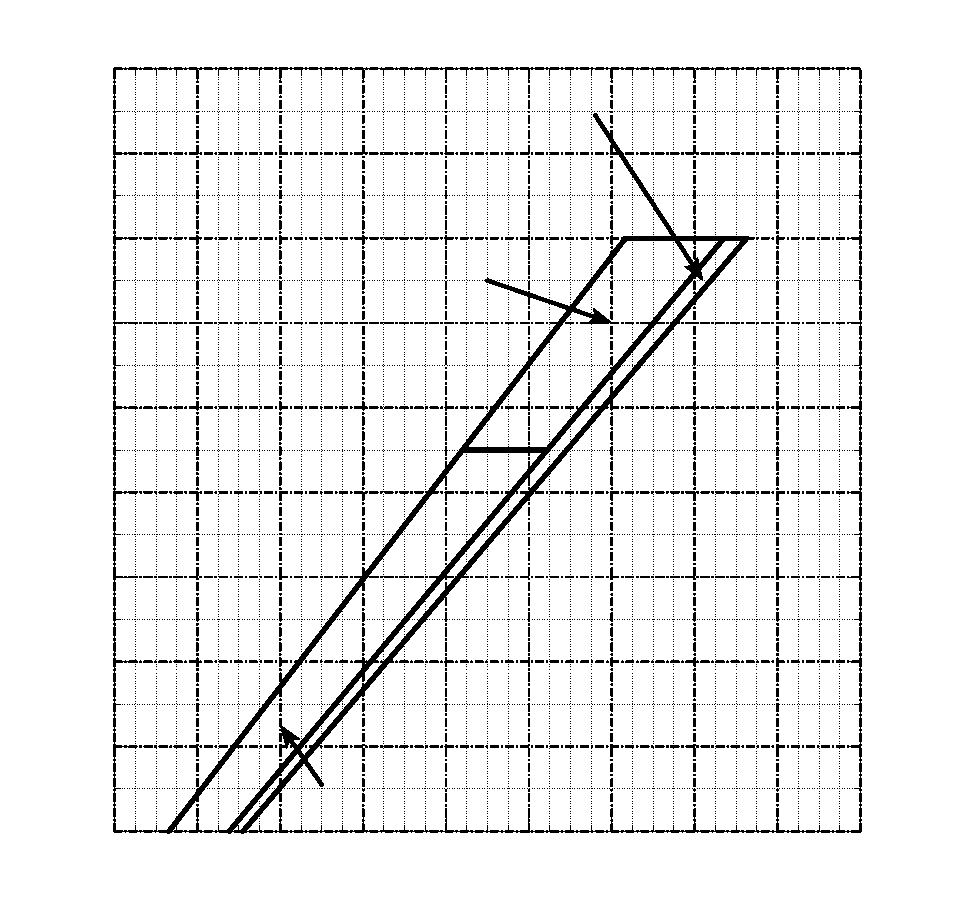
\includegraphics{../graphs/wb-moment-chart1800}}%
    \gplfronttext
  \end{picture}%
\endgroup
}
  \end{center}

\caption{CG Moment Envelope}
\label{CG-Moment}
\end{figure}

\begin{figure}
\addcontentsline{toc}{section}{Figure \ref{CG-chart} CG Limits}
\begin{center}
  \ifthenelse{\theMTOW > 1800}{% GNUPLOT: LaTeX picture with Postscript
\begingroup
  \makeatletter
  \providecommand\color[2][]{%
    \GenericError{(gnuplot) \space\space\space\@spaces}{%
      Package color not loaded in conjunction with
      terminal option `colourtext'%
    }{See the gnuplot documentation for explanation.%
    }{Either use 'blacktext' in gnuplot or load the package
      color.sty in LaTeX.}%
    \renewcommand\color[2][]{}%
  }%
  \providecommand\includegraphics[2][]{%
    \GenericError{(gnuplot) \space\space\space\@spaces}{%
      Package graphicx or graphics not loaded%
    }{See the gnuplot documentation for explanation.%
    }{The gnuplot epslatex terminal needs graphicx.sty or graphics.sty.}%
    \renewcommand\includegraphics[2][]{}%
  }%
  \providecommand\rotatebox[2]{#2}%
  \@ifundefined{ifGPcolor}{%
    \newif\ifGPcolor
    \GPcolorfalse
  }{}%
  \@ifundefined{ifGPblacktext}{%
    \newif\ifGPblacktext
    \GPblacktexttrue
  }{}%
  % define a \g@addto@macro without @ in the name:
  \let\gplgaddtomacro\g@addto@macro
  % define empty templates for all commands taking text:
  \gdef\gplbacktext{}%
  \gdef\gplfronttext{}%
  \makeatother
  \ifGPblacktext
    % no textcolor at all
    \def\colorrgb#1{}%
    \def\colorgray#1{}%
  \else
    % gray or color?
    \ifGPcolor
      \def\colorrgb#1{\color[rgb]{#1}}%
      \def\colorgray#1{\color[gray]{#1}}%
      \expandafter\def\csname LTw\endcsname{\color{white}}%
      \expandafter\def\csname LTb\endcsname{\color{black}}%
      \expandafter\def\csname LTa\endcsname{\color{black}}%
      \expandafter\def\csname LT0\endcsname{\color[rgb]{1,0,0}}%
      \expandafter\def\csname LT1\endcsname{\color[rgb]{0,1,0}}%
      \expandafter\def\csname LT2\endcsname{\color[rgb]{0,0,1}}%
      \expandafter\def\csname LT3\endcsname{\color[rgb]{1,0,1}}%
      \expandafter\def\csname LT4\endcsname{\color[rgb]{0,1,1}}%
      \expandafter\def\csname LT5\endcsname{\color[rgb]{1,1,0}}%
      \expandafter\def\csname LT6\endcsname{\color[rgb]{0,0,0}}%
      \expandafter\def\csname LT7\endcsname{\color[rgb]{1,0.3,0}}%
      \expandafter\def\csname LT8\endcsname{\color[rgb]{0.5,0.5,0.5}}%
    \else
      % gray
      \def\colorrgb#1{\color{black}}%
      \def\colorgray#1{\color[gray]{#1}}%
      \expandafter\def\csname LTw\endcsname{\color{white}}%
      \expandafter\def\csname LTb\endcsname{\color{black}}%
      \expandafter\def\csname LTa\endcsname{\color{black}}%
      \expandafter\def\csname LT0\endcsname{\color{black}}%
      \expandafter\def\csname LT1\endcsname{\color{black}}%
      \expandafter\def\csname LT2\endcsname{\color{black}}%
      \expandafter\def\csname LT3\endcsname{\color{black}}%
      \expandafter\def\csname LT4\endcsname{\color{black}}%
      \expandafter\def\csname LT5\endcsname{\color{black}}%
      \expandafter\def\csname LT6\endcsname{\color{black}}%
      \expandafter\def\csname LT7\endcsname{\color{black}}%
      \expandafter\def\csname LT8\endcsname{\color{black}}%
    \fi
  \fi
  \setlength{\unitlength}{0.0500bp}%
  \begin{picture}(9360.00,10080.00)%
    \gplgaddtomacro\gplbacktext{%
      \csname LTb\endcsname%
      \put(1210,704){\makebox(0,0)[r]{\strut{}1,100}}%
      \csname LTb\endcsname%
      \put(1210,1672){\makebox(0,0)[r]{\strut{}1,200}}%
      \csname LTb\endcsname%
      \put(1210,2640){\makebox(0,0)[r]{\strut{}1,300}}%
      \csname LTb\endcsname%
      \put(1210,3609){\makebox(0,0)[r]{\strut{}1,400}}%
      \csname LTb\endcsname%
      \put(1210,4577){\makebox(0,0)[r]{\strut{}1,500}}%
      \csname LTb\endcsname%
      \put(1210,5545){\makebox(0,0)[r]{\strut{}1,600}}%
      \csname LTb\endcsname%
      \put(1210,6513){\makebox(0,0)[r]{\strut{}1,700}}%
      \csname LTb\endcsname%
      \put(1210,7482){\makebox(0,0)[r]{\strut{}1,800}}%
      \csname LTb\endcsname%
      \put(1210,8450){\makebox(0,0)[r]{\strut{}1,900}}%
      \csname LTb\endcsname%
      \put(1210,9418){\makebox(0,0)[r]{\strut{}2,000}}%
      \csname LTb\endcsname%
      \put(1342,484){\makebox(0,0){\strut{} 78}}%
      \csname LTb\endcsname%
      \put(1996,484){\makebox(0,0){\strut{} 79}}%
      \csname LTb\endcsname%
      \put(2650,484){\makebox(0,0){\strut{} 80}}%
      \csname LTb\endcsname%
      \put(3305,484){\makebox(0,0){\strut{} 81}}%
      \csname LTb\endcsname%
      \put(3959,484){\makebox(0,0){\strut{} 82}}%
      \csname LTb\endcsname%
      \put(4613,484){\makebox(0,0){\strut{} 83}}%
      \csname LTb\endcsname%
      \put(5267,484){\makebox(0,0){\strut{} 84}}%
      \csname LTb\endcsname%
      \put(5921,484){\makebox(0,0){\strut{} 85}}%
      \csname LTb\endcsname%
      \put(6576,484){\makebox(0,0){\strut{} 86}}%
      \csname LTb\endcsname%
      \put(7230,484){\makebox(0,0){\strut{} 87}}%
      \csname LTb\endcsname%
      \put(7884,484){\makebox(0,0){\strut{} 88}}%
      \put(8016,704){\makebox(0,0)[l]{\strut{} 1100}}%
      \put(8016,1672){\makebox(0,0)[l]{\strut{} 1200}}%
      \put(8016,2640){\makebox(0,0)[l]{\strut{} 1300}}%
      \put(8016,3609){\makebox(0,0)[l]{\strut{} 1400}}%
      \put(8016,4577){\makebox(0,0)[l]{\strut{} 1500}}%
      \put(8016,5545){\makebox(0,0)[l]{\strut{} 1600}}%
      \put(8016,6513){\makebox(0,0)[l]{\strut{} 1700}}%
      \put(8016,7482){\makebox(0,0)[l]{\strut{} 1800}}%
      \put(8016,8450){\makebox(0,0)[l]{\strut{} 1900}}%
      \put(8016,9418){\makebox(0,0)[l]{\strut{} 2000}}%
      \put(1342,9638){\makebox(0,0){\strut{} 78}}%
      \put(1996,9638){\makebox(0,0){\strut{} 79}}%
      \put(2650,9638){\makebox(0,0){\strut{} 80}}%
      \put(3305,9638){\makebox(0,0){\strut{} 81}}%
      \put(3959,9638){\makebox(0,0){\strut{} 82}}%
      \put(4613,9638){\makebox(0,0){\strut{} 83}}%
      \put(5267,9638){\makebox(0,0){\strut{} 84}}%
      \put(5921,9638){\makebox(0,0){\strut{} 85}}%
      \put(6576,9638){\makebox(0,0){\strut{} 86}}%
      \put(7230,9638){\makebox(0,0){\strut{} 87}}%
      \put(7884,9638){\makebox(0,0){\strut{} 88}}%
      \put(308,5061){\rotatebox{-270}{\makebox(0,0){\strut{}Weight (lb)}}}%
      \put(8917,5061){\rotatebox{-270}{\makebox(0,0){\strut{}Weight (lb)}}}%
      \put(4613,154){\makebox(0,0){\strut{}CG (inches aft of datum)}}%
      \put(4613,9967){\makebox(0,0){\strut{}CG (inches aft of datum)}}%
    }%
    \gplgaddtomacro\gplfronttext{%
      \put(4456,7966){\makebox(0,0){\strut{}\Large \bfseries \sffamily Normal Weight/CG Envelope}}%
      \put(3959,6755){\makebox(0,0){\strut{}\Large \bfseries \sffamily Restricted Aerobatic}}%
      \put(3959,6271){\makebox(0,0){\strut{}\Large \bfseries \sffamily Weight/CG Envelope}}%
      \put(3959,4093){\makebox(0,0){\strut{}\Large \bfseries \sffamily Aerobatic Weight/CG Envelope}}%
    }%
    \gplbacktext
    \put(0,0){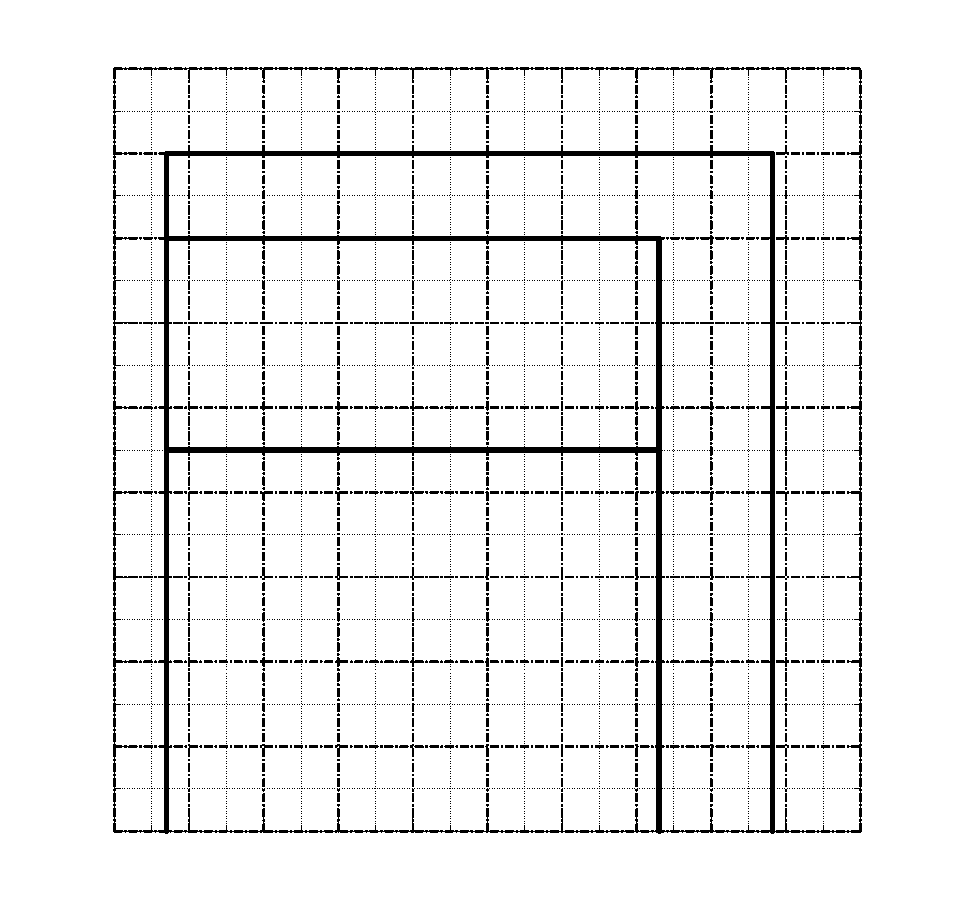
\includegraphics{../graphs/wb-cg-chart1900}}%
    \gplfronttext
  \end{picture}%
\endgroup
}{% GNUPLOT: LaTeX picture with Postscript
\begingroup
  \makeatletter
  \providecommand\color[2][]{%
    \GenericError{(gnuplot) \space\space\space\@spaces}{%
      Package color not loaded in conjunction with
      terminal option `colourtext'%
    }{See the gnuplot documentation for explanation.%
    }{Either use 'blacktext' in gnuplot or load the package
      color.sty in LaTeX.}%
    \renewcommand\color[2][]{}%
  }%
  \providecommand\includegraphics[2][]{%
    \GenericError{(gnuplot) \space\space\space\@spaces}{%
      Package graphicx or graphics not loaded%
    }{See the gnuplot documentation for explanation.%
    }{The gnuplot epslatex terminal needs graphicx.sty or graphics.sty.}%
    \renewcommand\includegraphics[2][]{}%
  }%
  \providecommand\rotatebox[2]{#2}%
  \@ifundefined{ifGPcolor}{%
    \newif\ifGPcolor
    \GPcolorfalse
  }{}%
  \@ifundefined{ifGPblacktext}{%
    \newif\ifGPblacktext
    \GPblacktexttrue
  }{}%
  % define a \g@addto@macro without @ in the name:
  \let\gplgaddtomacro\g@addto@macro
  % define empty templates for all commands taking text:
  \gdef\gplbacktext{}%
  \gdef\gplfronttext{}%
  \makeatother
  \ifGPblacktext
    % no textcolor at all
    \def\colorrgb#1{}%
    \def\colorgray#1{}%
  \else
    % gray or color?
    \ifGPcolor
      \def\colorrgb#1{\color[rgb]{#1}}%
      \def\colorgray#1{\color[gray]{#1}}%
      \expandafter\def\csname LTw\endcsname{\color{white}}%
      \expandafter\def\csname LTb\endcsname{\color{black}}%
      \expandafter\def\csname LTa\endcsname{\color{black}}%
      \expandafter\def\csname LT0\endcsname{\color[rgb]{1,0,0}}%
      \expandafter\def\csname LT1\endcsname{\color[rgb]{0,1,0}}%
      \expandafter\def\csname LT2\endcsname{\color[rgb]{0,0,1}}%
      \expandafter\def\csname LT3\endcsname{\color[rgb]{1,0,1}}%
      \expandafter\def\csname LT4\endcsname{\color[rgb]{0,1,1}}%
      \expandafter\def\csname LT5\endcsname{\color[rgb]{1,1,0}}%
      \expandafter\def\csname LT6\endcsname{\color[rgb]{0,0,0}}%
      \expandafter\def\csname LT7\endcsname{\color[rgb]{1,0.3,0}}%
      \expandafter\def\csname LT8\endcsname{\color[rgb]{0.5,0.5,0.5}}%
    \else
      % gray
      \def\colorrgb#1{\color{black}}%
      \def\colorgray#1{\color[gray]{#1}}%
      \expandafter\def\csname LTw\endcsname{\color{white}}%
      \expandafter\def\csname LTb\endcsname{\color{black}}%
      \expandafter\def\csname LTa\endcsname{\color{black}}%
      \expandafter\def\csname LT0\endcsname{\color{black}}%
      \expandafter\def\csname LT1\endcsname{\color{black}}%
      \expandafter\def\csname LT2\endcsname{\color{black}}%
      \expandafter\def\csname LT3\endcsname{\color{black}}%
      \expandafter\def\csname LT4\endcsname{\color{black}}%
      \expandafter\def\csname LT5\endcsname{\color{black}}%
      \expandafter\def\csname LT6\endcsname{\color{black}}%
      \expandafter\def\csname LT7\endcsname{\color{black}}%
      \expandafter\def\csname LT8\endcsname{\color{black}}%
    \fi
  \fi
  \setlength{\unitlength}{0.0500bp}%
  \begin{picture}(9360.00,10080.00)%
    \gplgaddtomacro\gplbacktext{%
      \csname LTb\endcsname%
      \put(1210,704){\makebox(0,0)[r]{\strut{} 1100}}%
      \csname LTb\endcsname%
      \put(1210,1672){\makebox(0,0)[r]{\strut{} 1200}}%
      \csname LTb\endcsname%
      \put(1210,2640){\makebox(0,0)[r]{\strut{} 1300}}%
      \csname LTb\endcsname%
      \put(1210,3609){\makebox(0,0)[r]{\strut{} 1400}}%
      \csname LTb\endcsname%
      \put(1210,4577){\makebox(0,0)[r]{\strut{} 1500}}%
      \csname LTb\endcsname%
      \put(1210,5545){\makebox(0,0)[r]{\strut{} 1600}}%
      \csname LTb\endcsname%
      \put(1210,6513){\makebox(0,0)[r]{\strut{} 1700}}%
      \csname LTb\endcsname%
      \put(1210,7482){\makebox(0,0)[r]{\strut{} 1800}}%
      \csname LTb\endcsname%
      \put(1210,8450){\makebox(0,0)[r]{\strut{} 1900}}%
      \csname LTb\endcsname%
      \put(1210,9418){\makebox(0,0)[r]{\strut{} 2000}}%
      \csname LTb\endcsname%
      \put(1342,484){\makebox(0,0){\strut{} 78}}%
      \csname LTb\endcsname%
      \put(1996,484){\makebox(0,0){\strut{} 79}}%
      \csname LTb\endcsname%
      \put(2650,484){\makebox(0,0){\strut{} 80}}%
      \csname LTb\endcsname%
      \put(3305,484){\makebox(0,0){\strut{} 81}}%
      \csname LTb\endcsname%
      \put(3959,484){\makebox(0,0){\strut{} 82}}%
      \csname LTb\endcsname%
      \put(4613,484){\makebox(0,0){\strut{} 83}}%
      \csname LTb\endcsname%
      \put(5267,484){\makebox(0,0){\strut{} 84}}%
      \csname LTb\endcsname%
      \put(5921,484){\makebox(0,0){\strut{} 85}}%
      \csname LTb\endcsname%
      \put(6576,484){\makebox(0,0){\strut{} 86}}%
      \csname LTb\endcsname%
      \put(7230,484){\makebox(0,0){\strut{} 87}}%
      \csname LTb\endcsname%
      \put(7884,484){\makebox(0,0){\strut{} 88}}%
      \put(8016,704){\makebox(0,0)[l]{\strut{} 1100}}%
      \put(8016,1672){\makebox(0,0)[l]{\strut{} 1200}}%
      \put(8016,2640){\makebox(0,0)[l]{\strut{} 1300}}%
      \put(8016,3609){\makebox(0,0)[l]{\strut{} 1400}}%
      \put(8016,4577){\makebox(0,0)[l]{\strut{} 1500}}%
      \put(8016,5545){\makebox(0,0)[l]{\strut{} 1600}}%
      \put(8016,6513){\makebox(0,0)[l]{\strut{} 1700}}%
      \put(8016,7482){\makebox(0,0)[l]{\strut{} 1800}}%
      \put(8016,8450){\makebox(0,0)[l]{\strut{} 1900}}%
      \put(8016,9418){\makebox(0,0)[l]{\strut{} 2000}}%
      \put(1342,9638){\makebox(0,0){\strut{} 78}}%
      \put(1996,9638){\makebox(0,0){\strut{} 79}}%
      \put(2650,9638){\makebox(0,0){\strut{} 80}}%
      \put(3305,9638){\makebox(0,0){\strut{} 81}}%
      \put(3959,9638){\makebox(0,0){\strut{} 82}}%
      \put(4613,9638){\makebox(0,0){\strut{} 83}}%
      \put(5267,9638){\makebox(0,0){\strut{} 84}}%
      \put(5921,9638){\makebox(0,0){\strut{} 85}}%
      \put(6576,9638){\makebox(0,0){\strut{} 86}}%
      \put(7230,9638){\makebox(0,0){\strut{} 87}}%
      \put(7884,9638){\makebox(0,0){\strut{} 88}}%
      \put(308,5061){\rotatebox{-270}{\makebox(0,0){\strut{}Weight (lb)}}}%
      \put(8917,5061){\rotatebox{-270}{\makebox(0,0){\strut{}Weight (lb)}}}%
      \put(4613,154){\makebox(0,0){\strut{}CG (inches aft of datum)}}%
      \put(4613,9967){\makebox(0,0){\strut{}CG (inches aft of datum)}}%
    }%
    \gplgaddtomacro\gplfronttext{%
      \put(6641,4093){\rotatebox{90}{\makebox(0,0){\strut{}\Large \bfseries \sffamily Normal Weight/CG Envelope}}}%
      \put(3959,6755){\makebox(0,0){\strut{}\Large \bfseries \sffamily Restricted Aerobatic}}%
      \put(3959,6271){\makebox(0,0){\strut{}\Large \bfseries \sffamily Weight/CG Envelope}}%
      \put(3959,4093){\makebox(0,0){\strut{}\Large \bfseries \sffamily Aerobatic Weight/CG Envelope}}%
    }%
    \gplbacktext
    \put(0,0){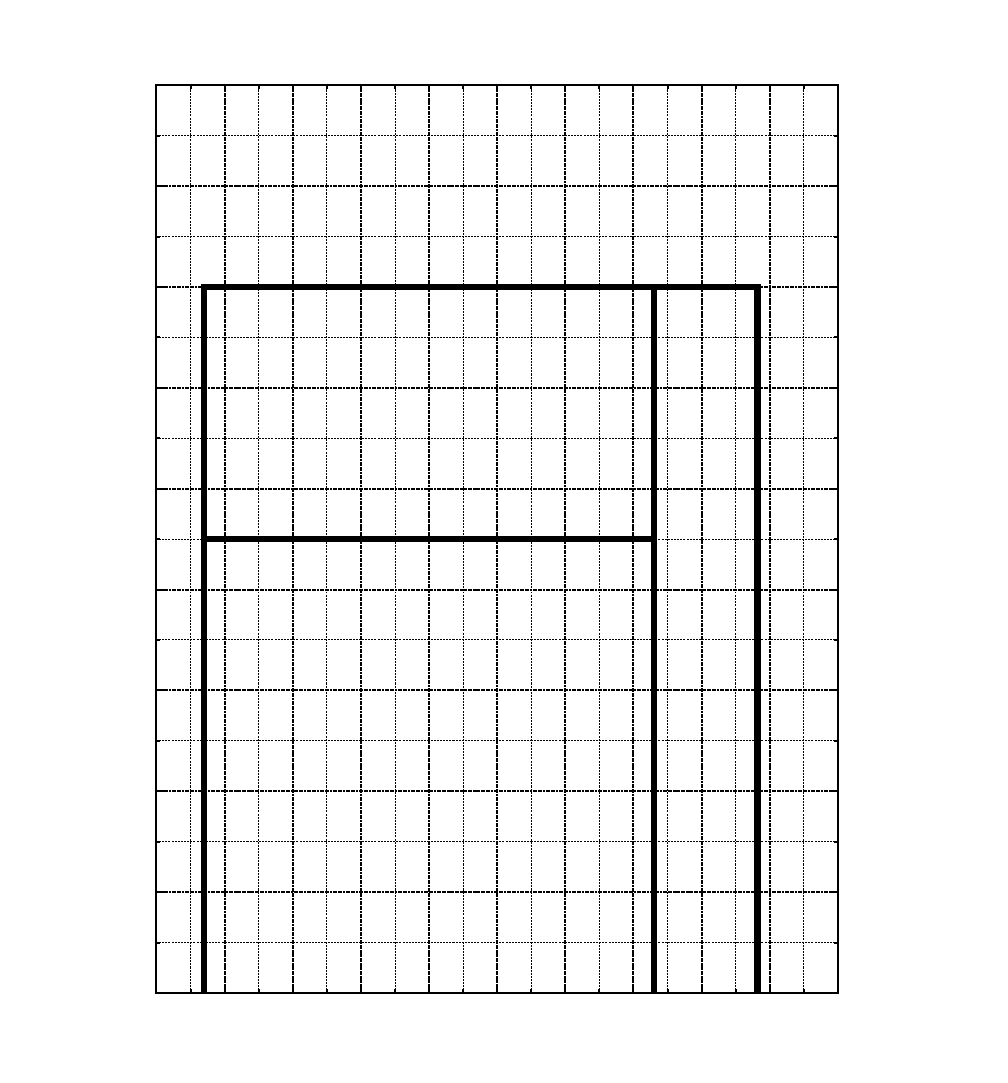
\includegraphics{../graphs/wb-cg-chart1800}}%
    \gplfronttext
  \end{picture}%
\endgroup
}
  \end{center}
\caption{CG Limits}
\label{CG-chart}
\end{figure}

\cleardoublepage

% !iTeXMac(input): POH.tex
\chapter{AIRPLANE \& SYSTEMS DESCRIPTIONS} \vspace{\minitocspacebefore} \minitoc

%\minilof
\cleardoublepage

%\startcontents[chapters]
%\titleformat{\chapter}[display] {...}{...}{...} % Your definitions come here [\vspace*{4pc}% 
%\startcontents[chapters] % from titletoc 
%\printcontents{l}{1}{\setcounter{tocdepth}{2}}] % from titletoc
%% following five commands to control the placement of figures on the pages
%% these values are changed for the Performance Section to allow room 
%% for two graphs on one page, with no text outside the figure.
\renewcommand{\textfraction}{0.1} 
\renewcommand{\topfraction}{.9} 
\renewcommand{\bottomfraction}{.9} 
\renewcommand{\floatpagefraction}{0.35} \setcounter{totalnumber}{5} 

\section{AIRFRAME}

The airframe is aluminum alloy construction except for steel components comprising: engine mount, landing gear, landing gear mounts, elevator control horns and other miscellaneous items. The tips of the wings and tail surfaces as well as cowling, landing gear fairings, empennage fairings and canopy skirt are fabricated from fibreglass. The aircraft is conventionally configured with a 13.5\% thick NACA 23000 series non-laminar-flow aerofoil.

\section{COCKPIT LAYOUT}

%\textcolor{red}{Finish adding legends for instrument panel diagram.}
The flight instruments are in a ``Standard-T'' arrangement, very slightly right of centre on the main instrument panel. The engine instruments and fuel gauges are to the right side of the flight instruments, and the avionics are located to the left of the flight instruments (Figure \ref{inst-panel}). Switches that are normally only used on the ground are on a switch console on the right cockpit wall below the instrument panel (Figure \ref{right-console}). Switches that are normally used in flight are on the sub-panel to the left of the main instrument panel (Figure \ref{left-sub-panel}).

The throttle, propeller and mixture controls are in a throttle quadrant mounted on the left cockpit wall below the instrument panel. The fuel selector is on a horizontal shelf on the lower, left side of the cockpit ahead of the pilot's seat.

Engine alternate air and oil cooler door controls are mounted on the side of the left landing gear box structure, below and ahead of the instrument panel. The cockpit heat controls are mounted on the aft wall of the forward baggage compartment, below and ahead of the instrument panel to the right of the pilot's right calf. 

The parking brake control is mounted on the centre of the forward baggage compartment aft bulkhead, below and ahead of the instrument panel.

The front stick grip contains controls for pitch and roll trim, trim and autopilot cut-out, boost pump ON-OFF toggle, radio transmit, and starter engage (Figure \ref{stick-grip}).

The auxiliary power outlet is located on the lower aft face of the right landing gear box structure.

The rear seat has a throttle mounted on the left side wall, and a pitch trim switch just ahead of the throttle. There is a radio transmit push-button near the top of the bulkhead on the right side of the rear cockpit. \clearpage \vspace*{\fill} 
\begin{center}
	
	%    This page intentionally left blank.
	\Large THIS PAGE INTENTIONALLY LEFT BLANK. 
\end{center}
\vspace{\fill} \thispagestyle{empty} 
\newpage 
\begin{sidewaysfigure}
	
	\begin{overpic}
		[scale=1]{../Diagrams/Panel7} \huge
		
		% The following commands work with the pspicture package
		% \put(24,37){\ding{172}} % #1 dingbat
		% \put(25.5,36.8){\Vector(.5,-7.8)}
		% \put(20,36){\ding{173}} % #2 dingbat
		% \put(22,35.9){\Vector(1.6,-6.9)}
		% \put(15,34){\ding{174}} % #3 dingbat
		% \put(17.3,34.3){\Vector(8,-8.5)}
		% \put(3,23){\ding{175}} % #4 dingbat
		% \put(5.5,23.7){\Vector(16.5,.8)}
		% \put(10.5,30){\ding{176}} % #5 dingbat
		% \put(13,30.7){\Vector(6.5,-4)}
		% \put(15,-5){\ding{177}} % #6 dingbat
		% \put(16.6,-2.3){\Vector(1.3,3.7)}
		% \put(20.1,-5){\ding{178}} % #7 dingbat
		% \put(21.3,-2.3){\Vector(0,3.7)}
		% \put(25.1,-5){\ding{179}} % #8 dingbat
		% \put(25.9,-2.3){\Vector(-1.3,3.7)}
		% \put(94,22){\ding{180}} % #9 dingbat
		% \put(94.2,22.1){\Vector(-2,-2.9)}
		% \put(95,-5){\ding{181}} % #10 dingbat
		% \put(95.8,-2.3){\Vector(-.6,3.7)}
		% \put(96.6,-2.3){\Vector(.5,3.7)}
		% The following commands work with the pict2e package
		\put(24,37){\ding{172}} 
		
		% #1 dingbat
		\put(25.5,36.8){\vector(5,-78){0.5}} \put(20,36){\ding{173}} 
		
		% #2 dingbat
		\put(22,35.9){\vector(16,-69){1.6}} \put(15,34){\ding{174}} 
		
		% #3 dingbat
		\put(17.3,34.3){\vector(80,-85){8}} \put(3,23){\ding{175}} 
		
		% #4 dingbat
		\put(5.5,23.7){\vector(165,8){16.5}} \put(10.5,30){\ding{176}} 
		
		% #5 dingbat
		\put(13,30.7){\vector(65,-40){6.5}} \put(15,-5){\ding{177}} 
		
		% #6 dingbat
		\put(16.6,-2.3){\vector(13,37){1.3}} \put(20.1,-5){\ding{178}} 
		
		% #7 dingbat
		\put(21.3,-2.3){\vector(0,1){3.7}} \put(25.1,-5){\ding{179}} 
		
		% #8 dingbat
		\put(25.9,-2.3){\vector(-13,37){1.3}} \put(94,22){\ding{180}} 
		
		% #9 dingbat
		\put(94.2,22.1){\vector(-20,-29){2}} \put(95,-5){\ding{181}} 
		
		% #10 dingbat
		\put(95.8,-2.3){\vector(-6,37){0.6}} \put(96.6,-2.3){\vector(5,37){0.5}} 
	\end{overpic}
	\vspace{.5in}
		\begin{multicols}
		{2} 
		\begin{enumerate*}
			\item \textbf{MSTR WARN} --- Flashes when the EIS 4000 Engine Monitor detects an exceedence. 
			\item \textbf{LOW OIL PRESSURE} --- Lights when the oil pressure is less than 15 psi. 
			\item \textbf{STRTR ENGAGED} --- Lights when the starter is engaged. 
			\item \textbf{BOOST PUMP} --- Lights when electrical power is supplied to the boost pump. 
			\item \textbf{ANNUN. BRT/DIM} --- Controls the annunciator and pitch and roll trim indicator intensity. \\
			Note: The MSTR WARN annunciator is not dimmable. 
			\item \textbf{INST PANEL} --- Dims panel floodlight and Microair 760 COM back-lighting. 
			\item \textbf{AVIONICS} --- Dims Garmin GNS 430W and transponder displays. 
			\item \textbf{CDI + ENG INST} --- Dims CDI, Narco 122D and Engine instruments. 
			\item \textbf{ELT REMOTE CONTROL} 
			\item \textbf{HEADSET JACKS} 
		\end{enumerate*}
	\end{multicols}
	\vspace{.5in} \caption{Instrument Panel} \label{inst-panel} 
\end{sidewaysfigure}
\clearpage
\begin{sidewaysfigure}
	\begin{minipage}{3in}
		
		\begin{overpic}
			[scale=.6, bb = 100 78 476 708]{../Diagrams/LH_Panel} \Huge \put(44,80){\ding{172}} 
			
			% #1 dingbat
			\put(41.3,67.1){\ding{173}} 
			
			% #2 dingbat
			\put(31.4,52.2){\ding{174}} 
			
			% #3 dingbat
			\put(29.4,23.7){\ding{175}} 
			
			% #4 dingbat
			\put(40.3,23.7){\ding{176}} 
			
			% #5 dingbat
			\put(51.2,23.7){\ding{177}} 
			
			% #6 dingbat
			\put(21.2,7.1){\ding{178}} 
			
			% #7 dingbat
			\put(29.7,7.1){\ding{179}} 
			
			% #8 dingbat
			\put(40.3,7.1){\ding{180}} 
			
			% #9 dingbat
			\put(51.2,7.1){\ding{181}} 
			
			% #10 dingbat
		\end{overpic}

	\end{minipage}
	\hfill 
	\begin{minipage}{5.6in} 
		\begin{enumerate}
			\item \textbf{FLUX VALVE} --- Selects the EFIS Flux Valve OFF if required due to electromagnetic interference with COM reception. 
			\item \textbf{PITCH TRIM INDICATOR} --- Displays Pitch Trim position. Nose Up trim is to the top of the display, Nose Down trim is to the bottom. 
			\item \textbf{ROLL TRIM INDICATOR} --- Displays roll trim position. 
			\item \textbf{NAV/STR} --- Controls Navigation and Strobe Lights. Lower position is Navigation and Strobe Lights OFF. Middle position is Navigation Lights ON, and Strobe Lights OFF. Upper position is Navigation Lights and Strobe Lights ON. 
			\item \textbf{TAXI LT} --- Controls Taxi Light in left outboard wing. 
			\item \textbf{LDG LT} --- Controls Landing Light in right outboard wing. \\
			\\
			The Taxi and Landing Lights flash alternately if both switches are placed in the middle, "FLASH", position. 
			\item \textbf{IGNITION --- MAG} --- Controls the single magneto. 
			\item \textbf{IGNITION --- ELEC} --- Controls the Electronic Ignition which is installed in place of the right magneto. 
			\item \textbf{STARTER} --- Guarded switch enables the Start switch on the front control stick grip, and provides an alternate starter switch. The lower position disables the stick grip starter switch. If the guard is lifted, and the switch placed in the middle position, the stick grip starter switch is enabled. The momentary upper position engages the starter. 
			\item \textbf{FLAPS} --- Momentary switch causes the flaps to move up or down while it is held. The flap actuator will free-wheel once the flaps reach full travel up or down. 
		\end{enumerate}
	\end{minipage}
\vspace{.5in} \caption{Instrument Panel --- Left Side} \label{left-sub-panel} 
\end{sidewaysfigure}
\FloatBarrier

\begin{wrapfigure}
	[26]{r}{150pt}
	\begin{overpic}
		[scale=0.5]{../Diagrams/RH-Console} \Large \put(5,91.5){1} \put(5,83.6){2} \put(5,75.7){3} \put(5,67.8){4} \put(5,59.9){5} \put(5,52){6} \put(5,44){7} \put(5,36.1){8} \put(5,28.2){9} \put(3.4,20.3){10} \put(3.4,12.4){11} \put(3.4,4.5){12}
	\end{overpic}
	\caption{Switch Console} \label{right-console} 
\end{wrapfigure}

\textbf{Right Console} --- The following switches are on the right console, which is located on the right wall of the cockpit, below the instrument panel:

\begin{enumerate}
	\item \textbf{BATT/ALT} --- Battery Master and Main Alternator switch. Left position is both OFF, middle position is Battery Master ON, and Main Alternator OFF, and right position is both ON. 
	\item \textbf{STBY ALT} --- Standby Alternator switch. 
	\item \textbf{ESS BUS FEED} --- NORM: Essential Bus is fed from Main Bus, via a diode. EMER: Essential Bus is fed directly from Battery. 
	\item \textbf{ENG INST} --- EIS 4000 Engine Monitor power switch. 
	\item \textbf{EFIS BU} --- Backup source of power for the EFIS, from the Battery Bus. 
	\item \textbf{TURN COORD} --- Turn Coordinator power switch, from the Battery Bus. 
	\item \textbf{PITOT HEAT} --- Pitot Heat power switch. 
	\item \textbf{DFRST FAN} --- Defrost Fan power switch. 
	\item \textbf{TRIM} --- Pitch and Roll Trim power. Also selects which pitch trim switches are enabled. 
	\item \textbf{WING LVLR} --- Autopilot power switch. Controls power to the Autopilot control head and servo. 
	\item \textbf{ALT} --- Main Alternator Field Circuit Breaker. This CB will pop if the Over-voltage Protection System detects an over-voltage, removing power from the alternator field, which shuts down the alternator. 
	\item \textbf{STBY ALT} --- Standby Alternator Relay CB. This CB will pop if the Over-voltage Protection System detects an over-voltage caused by the Standby Alternator. 
\end{enumerate}

\FloatBarrier

\clearpage 
\section{STICK GRIP SWITCHES}
\begin{figure}
	[h!]
	
	\begin{minipage}{3in}
	  The front seat has an Infinity Aerospace stick grip with switches that control various aircraft systems.
		\begin{enumerate}
			\item \textbf{Trim and Autopilot Disconnect} --- Red. The power to the elevator and aileron trim servos is removed when this momentary switch is depressed. The power will be restored when the switch is released.  A press and release within 5 seconds will disconnect the autopilot.  Holding the switch depressed for longer than 5 seconds will activate the autopilot Pilot Command Steering mode.
			
			\item \textbf{Elevator and Aileron Trim} --- Controls elevator and roll trim.
			
			\item \textbf{Boost Pump} --- Blue. The ON or OFF state of the boost pump power is toggled when this switch is pressed and released. The pump ON/OFF status is indicated by the "Boost Pump" light on the instrument panel which illuminates when the boost pump is powered.
			
			\item \textbf{Trigger} --- Not used. This Push ON, Push OFF switch may eventually be used for smoke system control. 
			
			\item \textbf{PTT} --- Black. Push to Talk.
			
			\item \textbf{Starter} --- Green. Engages the starter, if the Start Enable switch on the Instrument Panel is in the Enable position. 
		\end{enumerate}
	\end{minipage}
	%\qquad
	\quad 
	\begin{minipage}{2.85in}
		
		\begin{tabular}{cc} 
			\begin{overpic}[scale=.2]{../Diagrams/stick-grip1} \Large \put(-1,95){\ding{172}} 
				
				% #1 dingbat
				%  \put(3,94){\Vector(6,-12)}
				\put(3,94){\vector(1,-2){3.5}} \put(14.25,99.25){\ding{173}} 
				
				% #2 dingbat
				%  \put(19,99){\Vector(15,-13)}
				\put(19,99){\vector(6,-5){12}} \put(55,99){\ding{174}} 
				
				% #3 dingbat
				%  \put(56,98){\Vector(-3,-7)}
				\put(56,98){\vector(-1,-2){3}} \put(-1,60){\ding{176}} 
				
				% #5 dingbat
				%  \put(3,59){\Vector(4,-8)}
				\put(3,59){\vector(1,-2){4}} \normalsize 
			\end{overpic}
			&
			\begin{overpic}[scale=.17]{../Diagrams/stick-grip2} \Large \put(-6.25,43.25){\ding{175}} 
				
				% #4 dingbat
				%  \put(-2,48){\Vector(5,8)}
				\put(-2,48){\vector(2,4){4}} \put(1.5,35){\ding{177}} 
				
				% #6 dingbat
				%  \put(5,34){\Vector(7,-16)}
				\put(5,34){\vector(1,-2){7}} \normalsize 
			\end{overpic}
		\end{tabular}
		\caption{Stick Grip Switches} \label{stick-grip}
		
	\end{minipage}
\end{figure}
\FloatBarrier

\section{CANOPY}

\textbf{Canopy Latch} --- The canopy is latched by a handle and hook at the left front side of the sliding canopy frame. The handle may rotate and the hook may release if the handle is hit in flight, but the air loads push the canopy forward, so there is no risk of it departing the aircraft.

\textbf{Canopy Jettison} --- The front canopy bow is attached to the rollers by ``Pip'' pins that can be pulled by the pilot, thus allowing the front of the canopy to be released from the rails. The canopy jettison procedure is:
\begin{enumerate*}
	\item Canopy ``Pip'' pins --- PULL 
	\item Canopy Latch --- UNLATCH 
	\item Canopy --- PULL AFT and PUSH UP 
	\item Head --- DUCK to prevent getting hit by canopy as it departs the aircraft 
\end{enumerate*}
\begin{Note}
	[WARNING] The canopy may hit the tail as it departs the aircraft, so the canopy should only be jettisoned if it is intended to abandon the aircraft. 
\end{Note}

\section{ENGINE AND PROPELLER}

The aircraft is powered by a Lycoming I0-360-A1B6 four cylinder, direct drive, horizontally opposed engine rated at 200 HP at 2700 rpm. The engine is fitted with a 60 amp 14 volt main alternator, an 8 amp standby alternator, shielded magneto ignition, Lightspeed Engineering electronic ignition, fuel pump, fuel injection, and an alternate air induction system.

The exhaust system is all stainless steel with a crossover configuration and no mufflers. Two heat muffs provide cabin heat.

The engine drives a 72.05\char`\"{} (183 cm) diameter MT three-blade constant speed propeller.  The propeller blade roots have counterweights that force them towards coarse pitch if propeller governor oil pressure is lost.  The propeller blades are of composite construction, with a wooden core covered by epoxy fibreglass.  The outer portion of the blade leading edges is protected by a stainless steel erosion strip that is bonded in place.  The inner portion of the blade leading edge is protected by a self-adhesive strip.

\section{ENGINE MONITOR} 
\begin{wrapfigure}[15]{R}{0pt}
	
	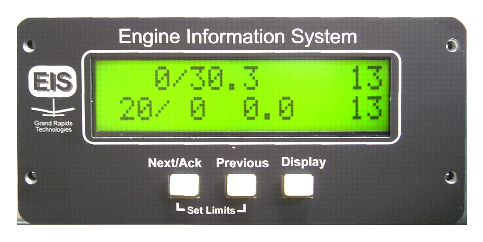
\includegraphics{../Diagrams/eis1} \caption{EIS 4000 Engine Monitor} 
\end{wrapfigure}

The Grand Rapids EIS 4000 Engine Information System (EIS) is located on the lower right side of the main instrument panel, and is powered from the Essential Bus, through the ``ENG INST'' switch on the right switch panel. The EIS 4000 displays the following engine parametres:
\begin{itemize*}
	\item RPM 
	\item Manifold Pressure (in HG) 
	\item Oil Temperature (\textdegree F) 
	\item Oil Pressure (\textdegree F) 
	\item Cylinder Head Temperature --- all cylinders (\textdegree F) 
	\item Exhaust Gas Temperatures --- all cylinders (\textdegree F) 
	\item Fuel Flow (USG/hr) 
	\item Fuel Remaining (USG) 
	\item Fuel Pressure ($\mathrm{lb/in^{2}}$) 
	\item Essential Bus Voltage (v)
	\item Outside Air Temperature (\textdegree F) from sensor mounted in NACA scoop under right wing. 
\end{itemize*}

\subsection*{Alarms}

%\textbf{Alarms} --- Each parametre that the EIS monitors can have upper and lower limits assigned, and the EIS will annunciate an alarm condition if these limits are breached.
Each parametre that the EIS monitors can have upper and lower limits assigned, and the EIS will annunciate an alarm condition if these limits are breached. The ``MSTR WARN'' red light will flash (upper left side of instrument panel), and the EIS display will change pages to show the affected parametre flashing above its label. If the parametre returns within the allowable range, the ``MSTR WARN'' light will extinguish, and the display will automatically return to the previously displayed page. The alarm can be reset by pressing the ``Next/Ack'' on the EIS. The ``MSTR WARN'' light will stop flashing, but will remain illuminated as long as any parametre remains outside the allowable range. The display will change to the previously displayed page.

\subsection*{Display Formats}

%\textbf{Displays} --- There are 14 different pages of data that may be displayed.  
There are 14 different pages of data that may be displayed. Pressing the ``Next/Ack'' button cycles to the next page. Pressing the ``Previous'' button cycles to the previous page. Double-pushing the ``Display'' button changes to the default page. The two user-configurable pages don't have labels identifying which parametre each block of numbers represents. Pressing and holding the ``Display'' button from a user-configurable page replaces the digits with the data labels, allowing the data blocks to be identified.
\clearpage 
The pages, in sequence, are:

% The following lengths define extra space to be left between the hlines and the text in the page format table.
\newlength{\tabletopspace} 
\setlength{\tabletopspace}{.5ex} 
\newlength{\tablebottomspace}
\setlength{\tablebottomspace}{.5ex}

% The following lengths control the table width
\newlength{\eistableleftcol} 
\setlength{\eistableleftcol}{1.2in}
% \settowidth{\eistableleftcol}{3:38 38.2 10.5 Endur Fuel Flow}
\newlength{\eistablerightcol} 
\setlength{\eistablerightcol}{\textwidth-\eistableleftcol-0.35in}
\begin{longtable}
	{|l|l|} \hline \multicolumn{1}{|c|}{\bfseries{EIS Page Layout}}&\multicolumn{1}{c|}{\bfseries{Remarks}}\\
	\hline\hline
\endfirsthead \multicolumn{2}{l}{\emph{Continued from previous page}}\\
\hline \multicolumn{1}{|c|}{\bfseries{EIS Page Layout}}&\multicolumn{1}{c|}{\bfseries{Remarks}}\\
\hline\hline 
\endhead \hline \multicolumn{2}{r}{\hfill \emph{Continued on next page}}\\
\endfoot \hline 
\endlastfoot

%% Fuel
\begin{minipage}{\eistableleftcol}\ttfamily 
\begin{verbatim}3:38  38.2  10.5
Endur Fuel  Flow\end{verbatim}
\end{minipage}&
\begin{minipage}{\eistablerightcol}
\vspace{\tabletopspace}
\textbf{Fuel Page }\\
\textbf{Top row} --- Endurance to dry tanks (H:M), Fuel Quantity (USG) and Fuel Flow (USG/hr).\\
\textbf{Bottom row} --- Data labels.

The fuel quantity is a detotalizer, based on the pilot-entered fuel quantity, less the integrated fuel flow.

% \centering \textbf{WARNING}
% 
% The fuel flow is not yet calibrated, so the detotalizer is not accurate.  \\
% The fuel gauges are the primary source of fuel quantity information.
\vspace{\tablebottomspace}
\end{minipage}\\
\hline

%%User page 1
\begin{minipage}{\eistableleftcol}
  \ttfamily {2410/23.0\ \ \ \ 400\\
200/70 10.5 1335} 
\end{minipage}
& 
\begin{minipage}{\eistablerightcol} 
  \vspace{
\tabletopspace} \textbf{User-configurable Page 1 --- Default Page}\\
\textbf{Top row} --- RPM/MP Highest CHT\\
\textbf{Bottom row} --- Oil Temperature/Oil Pressure, Fuel Flow (USG/hr), Highest EGT\\\\
Press and hold the ``Display'' button to replace the digits with data labels.\\
Double-push the ``Display'' button to switch to this page from any other page. \vspace{
\tablebottomspace} 
\end{minipage}
\\
\hline

%%User page 2
\begin{minipage}{\eistableleftcol}\ttfamily {36.8\ \ 10.8\ \ \ \ 29\\
-10\textdegree\ \ 13.6\ \ \ 0.0}
\end{minipage}&
\begin{minipage}{\eistablerightcol}
\vspace{\tabletopspace}
\textbf{User-configurable Page 2}\\
\textbf{Top row} --- Fuel Quantity (USG), Fuel Flow (USG/hr) and Fuel Pressure ($\mathrm{lb/in^{2}}$).\\
\textbf{Bottom row} --- OAT (\textdegree F), Essential Bus Voltage and Main Alternator Load (amps)\\\\
Press and hold the ``Display'' button to replace the digits with data labels.
\vspace{\tablebottomspace}
\end{minipage}\\
\hline

%%EGT/CHT Bar Graph Page
\begin{minipage}{\eistableleftcol}
\setlength{\unitlength}{1.31pt}
  \ttfamily {\begin{picture}(66,9)
    \linethickness{\unitlength}
    \put (0,0){\line(10,0){5}}
    \put (0,2){\line(10,0){5}}
    \put (0,4){\line(10,0){5}}
    \put (0,6){\line(10,0){5}}
    \put (6,0){\line(1,0){2}}
    \put (9,0){\line(1,0){2}}
    \put (6,2){\line(1,0){1}}
    \put (8,2){\line(1,0){3}}
    \put (6,4){\line(1,0){2}}
    \put (9,4){\line(1,0){2}}
    \put (6,6){\line(1,0){2}}
    \put (9,6){\line(1,0){2}}
    \put (12,0){\line(10,0){5}}
    \put (12,2){\line(10,0){5}}
    \put (12,4){\line(10,0){5}}
    \put (12,6){\line(10,0){5}}
    \put (18,0){\line(10,0){5}}
    \put (18,2){\line(10,0){5}}
    \put (18,4){\line(10,0){5}}
    \put (18,6){\line(10,0){5}}
    \put (24,0){\line(10,0){3}}
    \put (24,2){\line(10,0){1}}
    \put (24,4){\line(10,0){2}}
    \put (24,6){\line(10,0){4}}
    \put(40,0){2\ \ -50}
    \end{picture}
  \begin{picture}(66,9)
    \put(0,0){10.5 \ 1335 \ 2410}
    \end{picture}}
\end{minipage}&
\begin{minipage}{\eistablerightcol}
\vspace{\tabletopspace}
\textbf{EGT/CHT Bar Graph Page}\\
\textbf{Top row} --- EGT/CHT Bar Graph --- shows the EGT for each cylinder, with the CHT as a missing pixel.  
Then, the cylinder \# of the first cylinder to peak is shown, plus its change from the peak EGT. \\
\textbf{Bottom row} --- Fuel flow, EGT for first cylinder to peak and RPM.
\vspace{\tablebottomspace}
\end{minipage}\\
\hline

%%EGT Cruise Bar Graph Page
\begin{minipage}{\eistableleftcol}
\setlength{\unitlength}{1.31pt}
  \ttfamily {\begin{picture}(66,9)
    \linethickness{\unitlength}
    \put (16,6){\line(10,0){1}}
    \put (18,6){\line(10,0){5}}
    \put (24,0){\line(10,0){3}}
    \put (24,2){\line(10,0){1}}
    \put (24,4){\line(10,0){2}}
    \put(40,0){2\ \ -50}
    \end{picture}
  \begin{picture}(66,9)
    \put(0,0){10.5 \ 1335 \ 2410}
    \end{picture}}
\end{minipage}&
\begin{minipage}{\eistablerightcol}
\vspace{\tabletopspace}
\textbf{EGT Cruise Bar Graph Page}\\
\textbf{Top row} --- EGT Cruise Bar Graph --- shows how the EGT for each cylinder has changed from the saved lean point. 
Each pixel is 10\textdegree F.  Bars growing left of centre show decrease in EGT, to the right is an increase in EGT.  
Then, the cylinder \# of the first cylinder to peak is shown, then its EGT vs the peak EGT.\\
\textbf{Bottom row} --- Fuel flow, EGT for first cylinder to peak and RPM.
\vspace{\tablebottomspace}
\end{minipage}\\
\hline

%% EGT Page
\begin{minipage}{\eistableleftcol}\ttfamily 
  \begin{verbatim}1335 1325      E
1330 1325      G\end{verbatim}
\end{minipage}&
\begin{minipage}{\eistablerightcol}
\vspace{\tabletopspace}
\textbf{EGT Page }\\
\textbf{Top row} --- EGT \#2 EGT \#1\\
\textbf{Bottom row} ---  EGT \#4 EGT \#3\\\\
The EGT presentation is oriented as if the viewer was looking down on the engine.  I.e. the top row shows the EGTs for
the front two cylinders, and the bottom row shows the rear two cylinders.
\vspace{\tablebottomspace}
\end{minipage}\\
\hline

%% Digital Leaning Page
\begin{minipage}{\eistableleftcol}\ttfamily
  \begin{verbatim} -12  -25      2
 -15 1335      L
\end{verbatim}
\end{minipage}&
\begin{minipage}{\eistablerightcol}
\vspace{\tabletopspace}
\textbf{Digital Leaning Page }\\
\textbf{Top row} --- EGT \#2 EGT \#1\\
\textbf{Bottom row} ---  EGT \#4 EGT \#3\\\\
Shows the EGTs for all cylinders that have not peaked.  
Once an EGT reaches peak, and decreases by 10\textdegree F, the EGT is replaced by the amount the temperature has
decreased from the peak.  
The cylinder \# for the first cylinder to peak is shown in the top right corner of the display.  \textbf{Note that the
numbering scheme here is not the same as Lycoming's cylinder numbering scheme} --- 1 is top left (Cyl \#2), 2 is top right (Cyl \#1), 3 is bottom left (Cyl \#4) and 4 is bottom right (Cyl \#3). 
\vspace{\tablebottomspace}
\end{minipage}\\
\hline

%% Cruise Page
\begin{minipage}{\eistableleftcol}\ttfamily
\begin{verbatim} -12   15      C
  10    5      Z\end{verbatim}
\end{minipage}&
\begin{minipage}{\eistablerightcol}
\vspace{\tabletopspace}
\vspace{.25ex}
\textbf{Cruise Page }\\
\textbf{Top row} --- EGT \#2 EGT \#1\\
\textbf{Bottom row} ---  EGT \#4 EGT \#3\\\\
Shows the amount the EGTs have changed since ``SAVE LEAN PT.'' was selected.
\vspace{.25ex}
\vspace{\tablebottomspace}
\end{minipage}\\
\hline

%% CHT Page
\begin{minipage}{\eistableleftcol}\ttfamily 
\begin{verbatim} 385  400    400
 390  395    CHT\end{verbatim}
\end{minipage}&
\begin{minipage}{\eistablerightcol}
\vspace{\tabletopspace}
\textbf{CHT Page }\\
\textbf{Top row} --- CHT \#2 CHT \#1  plus highest CHT in top right corner.\\
\textbf{Bottom row} ---  CHT \#4 CHT \#3\\\\
The CHT presentation is oriented as if the viewer was looking down on the engine.  I.e. the top row shows the CHT for
the front two cylinders, and the bottom row shows the rear two cylinders. 
\vspace{\tablebottomspace}
\end{minipage}\\
\hline

%% Flight Timer Page
\begin{minipage}{\eistableleftcol}\ttfamily 
1:22:57\ \ \ \ \ 108\textdegree \\
191.5 Hour\ \ Unit
\end{minipage}&
\begin{minipage}{\eistablerightcol}
\vspace{\tabletopspace}
\textbf{Timer/Temperature Page }\\
\textbf{Top row} --- Flight Timer --- runs when the RPM is above 2000 rpm.  Shows the last flight time at power up, and
the current flight time after three minutes of flight.  Hours:Minutes:Seconds.  The internal unit temperature is shown
in the top right corner.\\
\textbf{Bottom row} --- Engine Hours --- accumulates when the RPM is above 2000 rpm. 
\vspace{\tablebottomspace}
\end{minipage}\\
\hline

%% RPM, OT & OP
\begin{minipage}{\eistableleftcol}\ttfamily 
\begin{verbatim}2410  195     82
RPM   OilT  OilP\end{verbatim}
\end{minipage}&
\begin{minipage}{\eistablerightcol}
\vspace{\tabletopspace}
\textbf{RPM, Oil Temperature and Oil Pressure Page }\\
\textbf{Top row} --- RPM, Oil Temperature (\textdegree F) and Oil Pressure ($\mathrm{lb/in^{2}}$).\\
\textbf{Bottom row} --- Data labels.
\vspace{\tablebottomspace}
\end{minipage}\\
\hline

%% MP & Fuel Pressure
\begin{minipage}{\eistableleftcol}\ttfamily 
\begin{verbatim}24.6    0   32.0
MP           FP\end{verbatim}
\end{minipage}&
\begin{minipage}{\eistablerightcol}
\vspace{\tabletopspace}
\textbf{Manifold and Fuel Pressure Page }\\
\textbf{Top row} --- Manifold Pressure (in HG), Aux 2 input (not used) and Fuel Pressure ($\mathrm{lb/in^{2}}$).\\
\textbf{Bottom row} --- Data labels.
\vspace{\tablebottomspace}
\end{minipage}\\
\hline

%% OAT & Voltage
\begin{minipage}{\eistableleftcol}\ttfamily 
\begin{verbatim} 24   13.4   0.0
OAT   Volt  Load\end{verbatim}
\end{minipage}&
\begin{minipage}{\eistablerightcol}
\vspace{\tabletopspace}
\textbf{OAT, Voltage and Alternator Load Page }\\
\textbf{Top row} --- OAT (\textdegree F), Essential Bus Voltage and Main Alternator Load (amps).\\
\textbf{Bottom row} --- Data labels.
\vspace{\tablebottomspace}
\end{minipage}\\
\hline

%% CRate & EGT Span
\begin{minipage}{\eistableleftcol}\ttfamily 
\begin{verbatim} 13    45    -28
CRate EGTSp Carb\end{verbatim}
\end{minipage}&
\begin{minipage}{\eistablerightcol}
\vspace{\tabletopspace}
\textbf{CHT Rate of Cooling and EGT Span Page }\\
\textbf{Top row} --- Cylinder Head rate of cooling (\textdegree F/mn) and EGT Span between hottest and coolest EGT
(\textdegree F).\\
\textbf{Bottom row} --- Data labels.

\centering NOTE\\
Ignore the data labelled ``Carb''.  It is not operative.
\vspace{\tablebottomspace}
\end{minipage}\\
\hline

\end{longtable}

\begin{Note}
The tachometer signal is from the Magneto. The RPM will read "0" if the IGNITION --- MAG switch is selected OFF. 
\end{Note}

\subsection*{Setting Alarm Limits}
The upper and lower alarm limits, and other user-modifiable data, may be edited via the ``Set Limits'' function, accessed by pressing and holding the ``Next/Ack'' and `` Previous'' buttons. This brings up a long series of pages where individual parametres may be adjusted, using ``soft'' labels above each of the EIS keys. After the desired parametres are modified, normal operation is resumed by pressing and holding the ``Display'' button (which will have a soft label of ``Next'') to quickly scroll through the pages until the final page is reached, or by cycling the EIS power OFF then ON, via the ENG INST switch on the right console.

\subsection*{Normal Operation}

After power-up, the EIS will alarm for any parametres that are outside the allowable limits, such as oil pressure, fuel pressure, etc. Acknowledge each alarm in turn by a momentary press of the ``Next/Ack'' button. The unit will default to the User-Configurable Page 1, which has RPM, MP, highest CHT and EGT, Oil Pressure, Oil Temperature and Fuel Flow. Pressing and holding the ``Display'' button will replace the data with the data labels, so each field may be identified. A press of the ``Next/Ack'' button will bring up User-Configurable Page 2, which has Fuel Quantity, Fuel Flow, Fuel Pressure, OAT, Voltage and Main Alternator Load. There are 14 different pages in all --- a double-push of the ``Display'' button will return to the default page.

\textbf{Fuel Detotalizer} --- Upon power-up the fuel detotalizer function will start with the fuel quantity it had at the last power-down.  Press and hold the left and right buttons to reach the fuel quantity page.  Once on the fuel quantity page, the fuel quantity may be adjusted as indicated by the ``Soft'' labels.  The fuel quantity can be quickly set to 43 USG (full tanks) by simultaneously pushing the buttons indicated by the ``Inc'' and ``Dec'' labels.  

\textbf{Digital Leaning Page} --- The digital leaning page is a special page that is intended to be used when leaning the mixture. This page is identified by the ``L'' in the lower right corner. Initially it shows the highest EGT for each cylinder, until each cylinder's EGT peaks, in which case it shows the EGT decrease from peak. The first cylinder to peak is identified by the digit in the top right corner of the window. Note that the numbering scheme here is not the same as Lycoming's cylinder numbering scheme --- 1 is top left (Cyl \#2), 2 is top right (Cyl \#1), 3 is bottom left (Cyl \#4) and 4 is bottom right (Cyl \#3). 

The page is used as follows: 
\begin{enumerate}
\item Select the Digital Lean Page, identified by the ``L'' in the lower right corner. 
\item Select the ``Save Lean Point?'' window, by a momentary press of the centre and right buttons, and select ``RESET''. This resets the highest EGTs to the current values. 
\item Slowly lean the engine. The EGTs should all increase, and the highest EGT for each cylinder will be continually updated. 
\item As leaning continues, one cylinder will reach peak EGT. Once the EGT was decreased by 10\textdegree F below peak the display will change to now show the number of degrees that the cylinder is less than the peak EGT. The first cylinder to peak is identified by the digit in the top right corner of the window. Note that the numbering scheme here is not the same as Lycoming's cylinder numbering scheme --- 1 is top left (Cyl \#2), 2 is top right (Cyl \#1), 3 is bottom left (Cyl \#4) and 4 is bottom right (Cyl \#3).  
\item Enrichen or lean as desired so all cylinders are at the desired value lower than the peak EGT.
\end{enumerate}

\subsection*{Abnormal Operations} The EIS will flash the ``MSTR WARN'' red light if any parametre goes outside the upper or lower limits programmed via the ``Set Limits'' interface. The EIS display will automatically change to a page that displays the parametre of interest, with the value flashing.  Press the ``Next/Ack'' button to acknowledge the warning --- the EIS display will return to its previous page.  The ``MSTR WARN'' light will stop flashing, but will remain illuminated until all parametres are within the programmed ranges.  If another parametre goes outside the programmed ranges, the ``MSTR WARN'' light will flash again, and the display will change to show the parametre of interest.

\section{ENGINE CONTROLS} Engine controls consist of throttle, propeller, mixture, alternate air door and oil cooler door controls. The throttle, propeller and mixture controls are in a throttle quadrant mounted on the left side of the front cockpit. The alternate air door position is controlled by a push-pull Bowden cable connected to a knob mounted on the upper, inboard side of the left landing gear box structure, underneath and ahead of the instrument panel. The oil cooler door controls the amount of air that enters the oil cooler, to allow the oil temperature to be varied. The oil cooler door position is controlled by a push-pull Bowden cable connected to a knob mounted on the upper, inboard side of the left landing gear box structure, underneath and ahead of the instrument panel.

\section{LANDING GEAR} The landing gear is of conventional configuration with steel landing gear legs. The tail wheel is full castering --- it is normally locked and follows the rudder position, but unlocks to a castering condition if full rudder is applied.

The main gear wheels are fitted with Cleveland 199-102 wheels and disk brakes. The tail wheel is solid rubber.

\section{BRAKES} The braking system consists of toe brakes attached to the rudder pedals operating two Cleveland brake master cylinders. The left and right brake master cylinders share a common fluid reservoir installed on the top left front face of the fire wall. Care must be taken to avoid applying brake pressure when using rudder on the ground.

%Both brake pedals should have a similar feel and a firm resistance
%after \textcolor{yellow}{\_}\char`\"{} of pedal travel.
The parking brake control valve is mounted on the forward baggage compartment aft bulkhead, below and forward of the instrument panel. The valve cannot be seen with the head in the normal flying position, but it can be felt if the hand is placed below the instrument panel, and it can be seen if the head is lowered. The control lever is on the left side of the braking brake valve, and has a spring loaded catch to secure it in the OFF position. The parking brake is OFF if the control lever is rotated vertically upwards, and it is ON if the control lever is rotated vertically downwards. 
\begin{Note}
[WARNING] The parking brake valve must be checked prior to landing to ensure that it is held in the OFF position by the spring-loaded catch. If the parking brake valve is in the ON position, any applied brake cannot be released, which may lead to loss of directional control. 
\end{Note}
\begin{Note}
[WARNING] The brakes have enough brake energy capacity for a single maximum braked rejected take-off or landing from normal approach speed.  Multiple hard braking events, or a maximum braked landing from an abnormally high landing speed could overheat the brakes resulting in brake failure. 
\end{Note}

\textcolor{red}{ADD PHOTO OR DRAWING OF PARKING BRAKE VALVE LOCATION}

\section{FLIGHT CONTROLS}

%Flight control integrity is essential for safe flight. At installation
%or after maintenance it should be confirmed that ALL controls are
%connected, secured and safeties and that they all operate within the
%specified ranges smoothly and in the correct direction. Full travel
%should be confirmed prior to each flight. NO play should be permitted
%in the control hinges; sloppiness may induce flutter. Similarly trim
%tabs must be free of play. 
%
Dual controls are fitted. A pin at the base of the passenger control stick allows it to be removed without affecting the operation of the remaining controls. Elevator and ailerons are operated through a system of adjustable push rods. The rudder is operated through a cable system to the rudder pedals.
%Rudder control from the rear seat position is by pads connected to push rods that are connected to the rudder cables. 

Pitch trim is by a tab on the right elevator actuated by an electric servo. Roll trim is by a spring bungee system actuated by an electric servo. Pitch and roll trim are selected by a ``Coolie Hat'' switch on the pilot's stick grip. Pitch trim can also be selected by a spring loaded switch ahead of the rear seat throttle lever. Trim positions are shown on LCD indicators located on the upper left portion of the instrument panel. Trim system power can be selected to OFF, FRONT or FRONT + REAR by a three position switch on the right console. Trim system power will also be removed while the red TRIM + WING LEVELER cut-out switch on the pilot's stick is depressed.

Flaps are operated electrically and are controlled by a switch mounted on the left side of the instrument panel.

\section{FUEL SYSTEM} Fuel is stored in two 21.5 US gallon tanks secured to the leading edge structure with screws and plate nuts. Fuel drains are fitted to the lowest point of each tank (and of the fuel system) and should be opened prior to the first flight of the day and after each refuelling to check for sediment and water.

The left tank is fitted with an inverted fuel pickup, which is a weighted length of flexible line, with a fuel pickup at the loose end. This introduces additional failure modes for the left tank --- the fuel pickup could get hung up inside the tank, or it could become disconnected at the front end. These failures would increase the amount of unusable fuel in the left tank by several gallons.
\begin{Note}
[WARNING] Never assume that all fuel in the left tank is usable. The left tank must not be selected for takeoff or landing unless there are at least \textcolor{red}{10 USG} of fuel remaining in that tank. If it is planned to use most of the fuel on a flight, the left tank must be used to a low value while adequate fuel still remains in the right fuel tank to safely land the aircraft in case the left fuel tank feed ceases prematurely. 
\end{Note}

The fuel selector valve is located to the left of the pilot's seat on the lower console. A knob on the valve handle must be lifted to change the selection to or from the OFF position.

A fuel gascolator is located in the left wing root area. This is not the lowest point in the fuel system and is intended as a dirt trap only prior to fuel entering the fuel pumps. The gascolator should be drained prior to the first flight of the day --- the fuel selector must be selected to LEFT or RIGHT to allow fuel to flow through the gascolator so it can be drained.

An electric boost pump is fitted in case of failure of the engine-driven fuel pump and is also used during takeoff and landing. The boost pump is controlled by the green ON/OFF toggle push button on the pilot's control stick. The green boost pump lamp on the upper left instrument panel will illuminate when electrical power is supplied to the boost pump.

The fuel filter is located on the engine side of the firewall, and is in the system between the boost pump and the engine-driven fuel pump.

A fuel flow transducer is fitted between the engine-driven fuel pump and the fuel injection servo. The fuel flow information is fed to the Grand Rapids EIS 4000, which has a detotalizer function that calculates predicted fuel remaining. The fuel quantity information in the EIS 4000 must be updated whenever fuel is added to or drained from the fuel tanks.
\begin{Note}[WARNING]The displayed fuel remaining value does not take into account any possible fuel leaks, or erroneous input of starting fuel quantity. 
\end{Note}

A fuel pressure transducer is mounted between the engine-driven fuel pump and the fuel injection servo. The fuel pressure is monitored and alarmed by the Grand Rapids EIS 4000.
\begin{figure}
[hb!] 
\begin{center}
\includegraphics*[scale = 0.4]{../Diagrams/Fuel_system4}
\end{center}

%\scalebox{.4}{\input{../Diagrams/Fuel_system5}}
%\input{../Diagrams/Fuel_system5}
\caption{Fuel System} 
\end{figure}
\clearpage 

%force fuel system figure to appear, before moving on to next system
\section{ELECTRICAL SYSTEM} 
\begin{wrapfigure}
[40]{R}{0pt} 
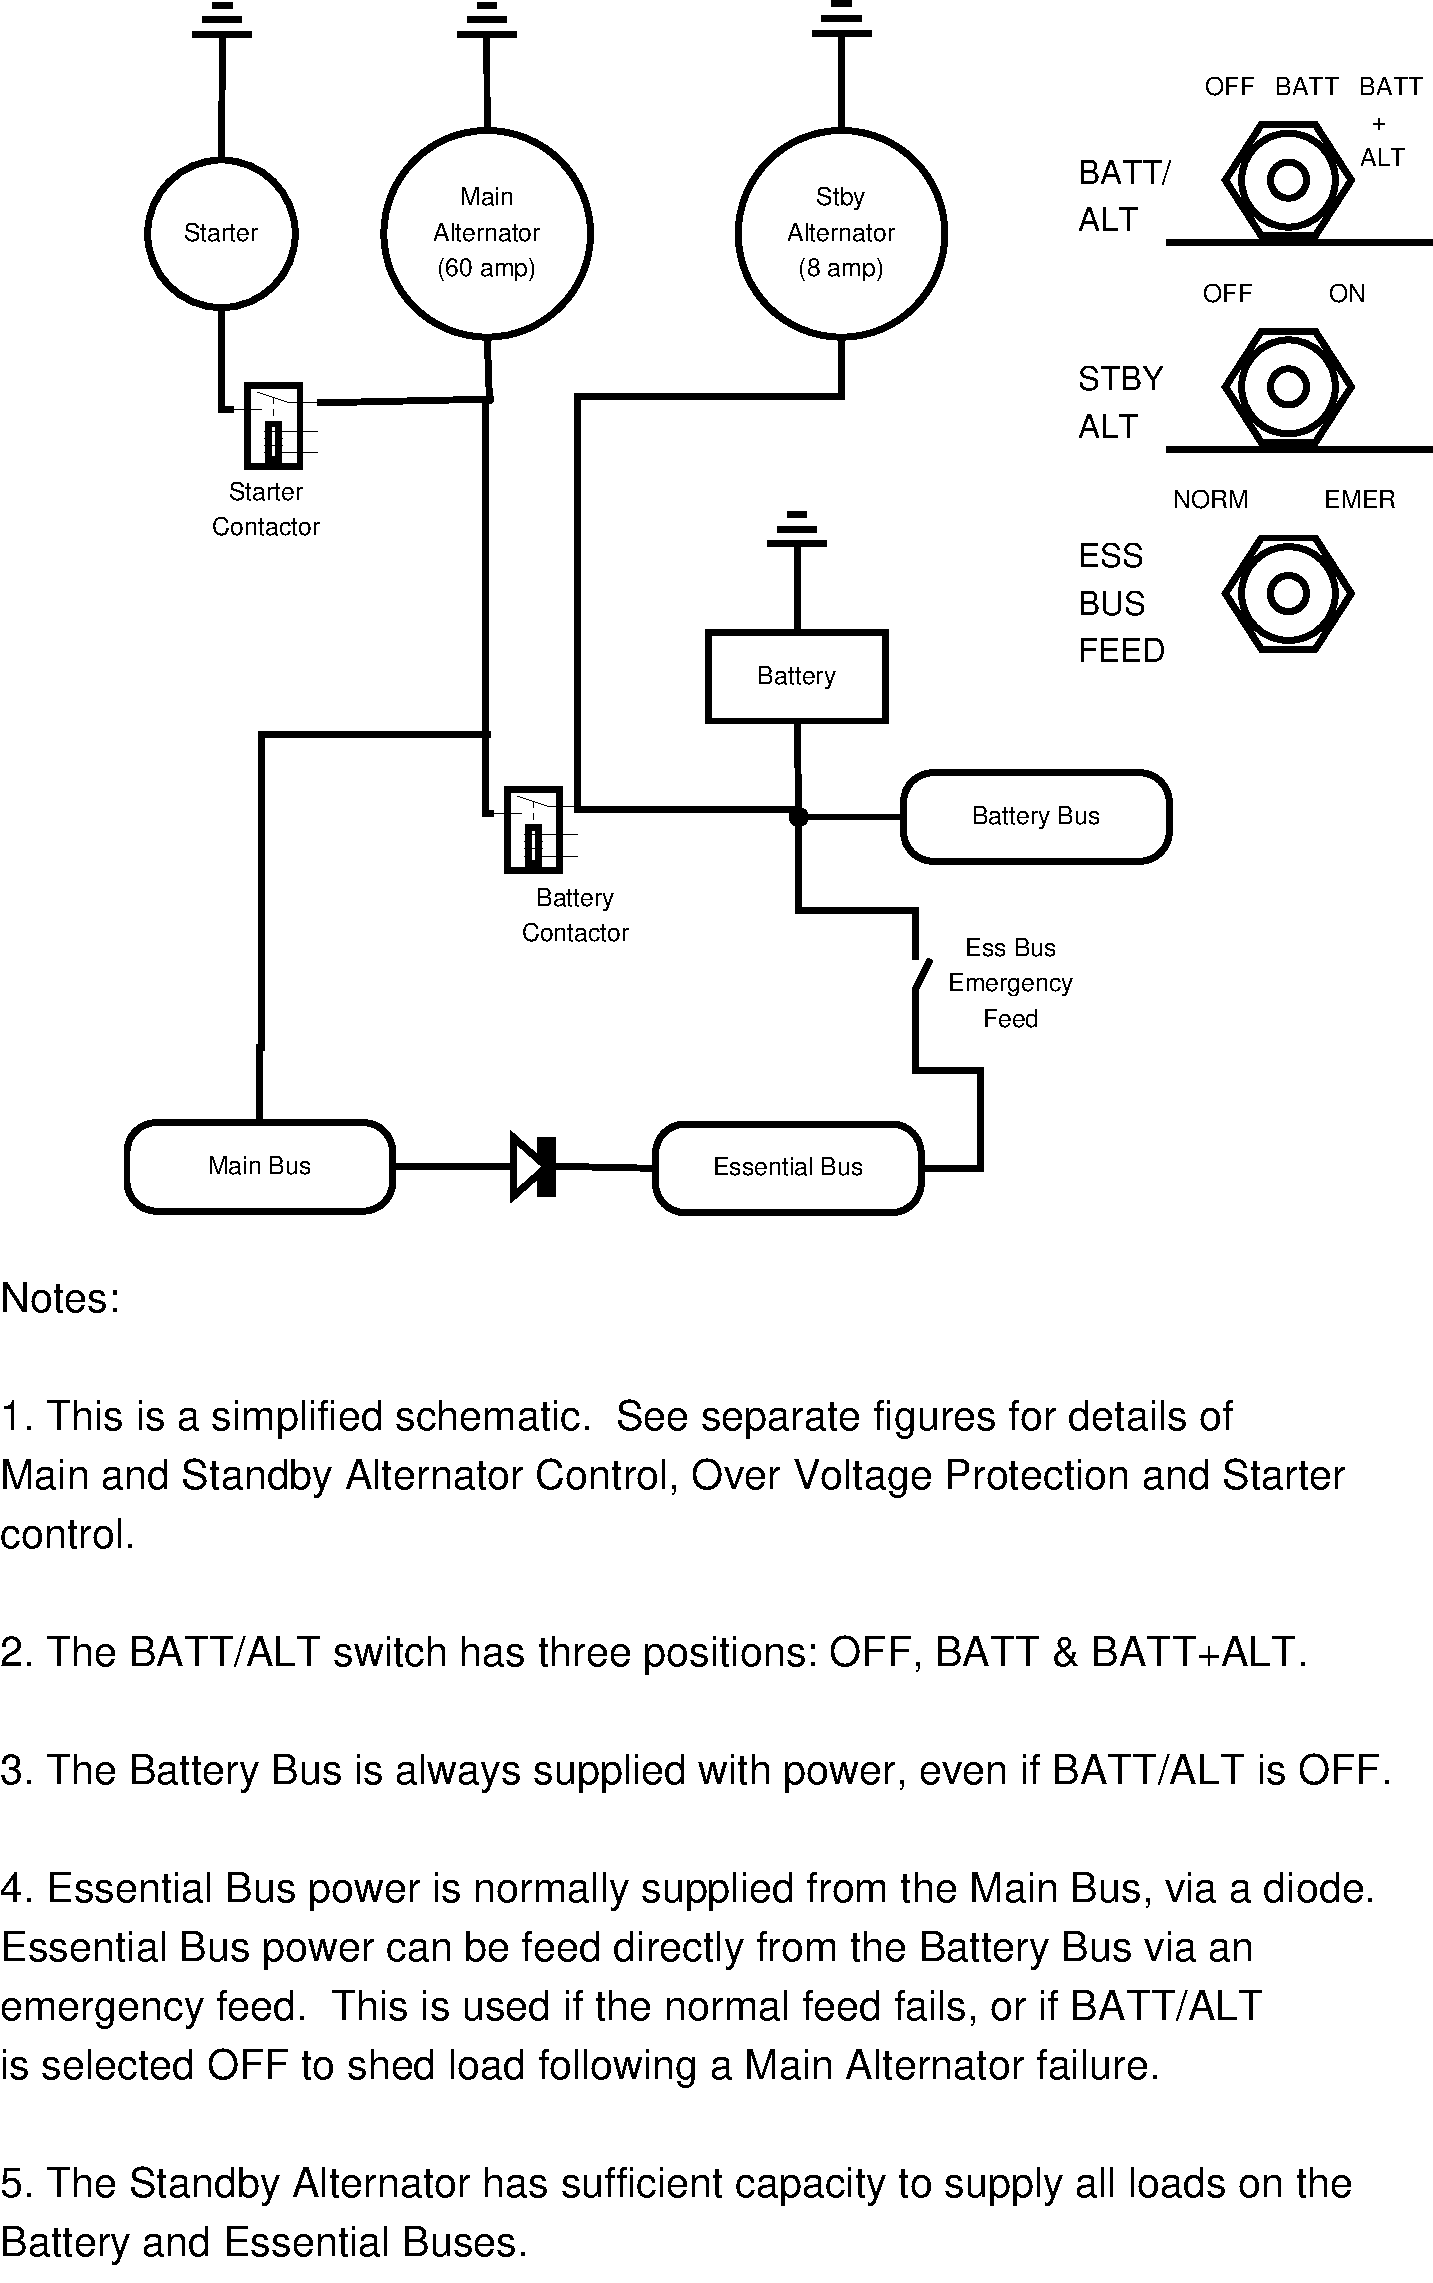
\includegraphics[clip,scale=0.4]{../Diagrams/Electrical_system_large_note} \caption{Electrical System} 
\end{wrapfigure}

The electrical system includes a 14 volt 60 amp Main Alternator, a 12 volt, 17 amp-hour battery, over voltage protection, an 8 amp Standby Alternator and a Battery Contactor. Power is distributed to Main, Essential and Battery Buses. Normally the Main Bus is powered from the Battery and Main Alternator, and the Essential Bus is powered from the Main Bus via a diode. The Battery Bus is powered all the time, regardless of the state of the Battery Contactor. The Essential Bus has a selectable alternate feed path from the Battery Bus. This alternate feed path is used if the power supplied from the Main Bus has failed, or if the Main Bus is manually shed following Main Alternator failure. An Aux Power outlet provides 10A of Battery Bus power for handheld devices. It may also be used to charge the battery.

\begin{figure}
\centering 
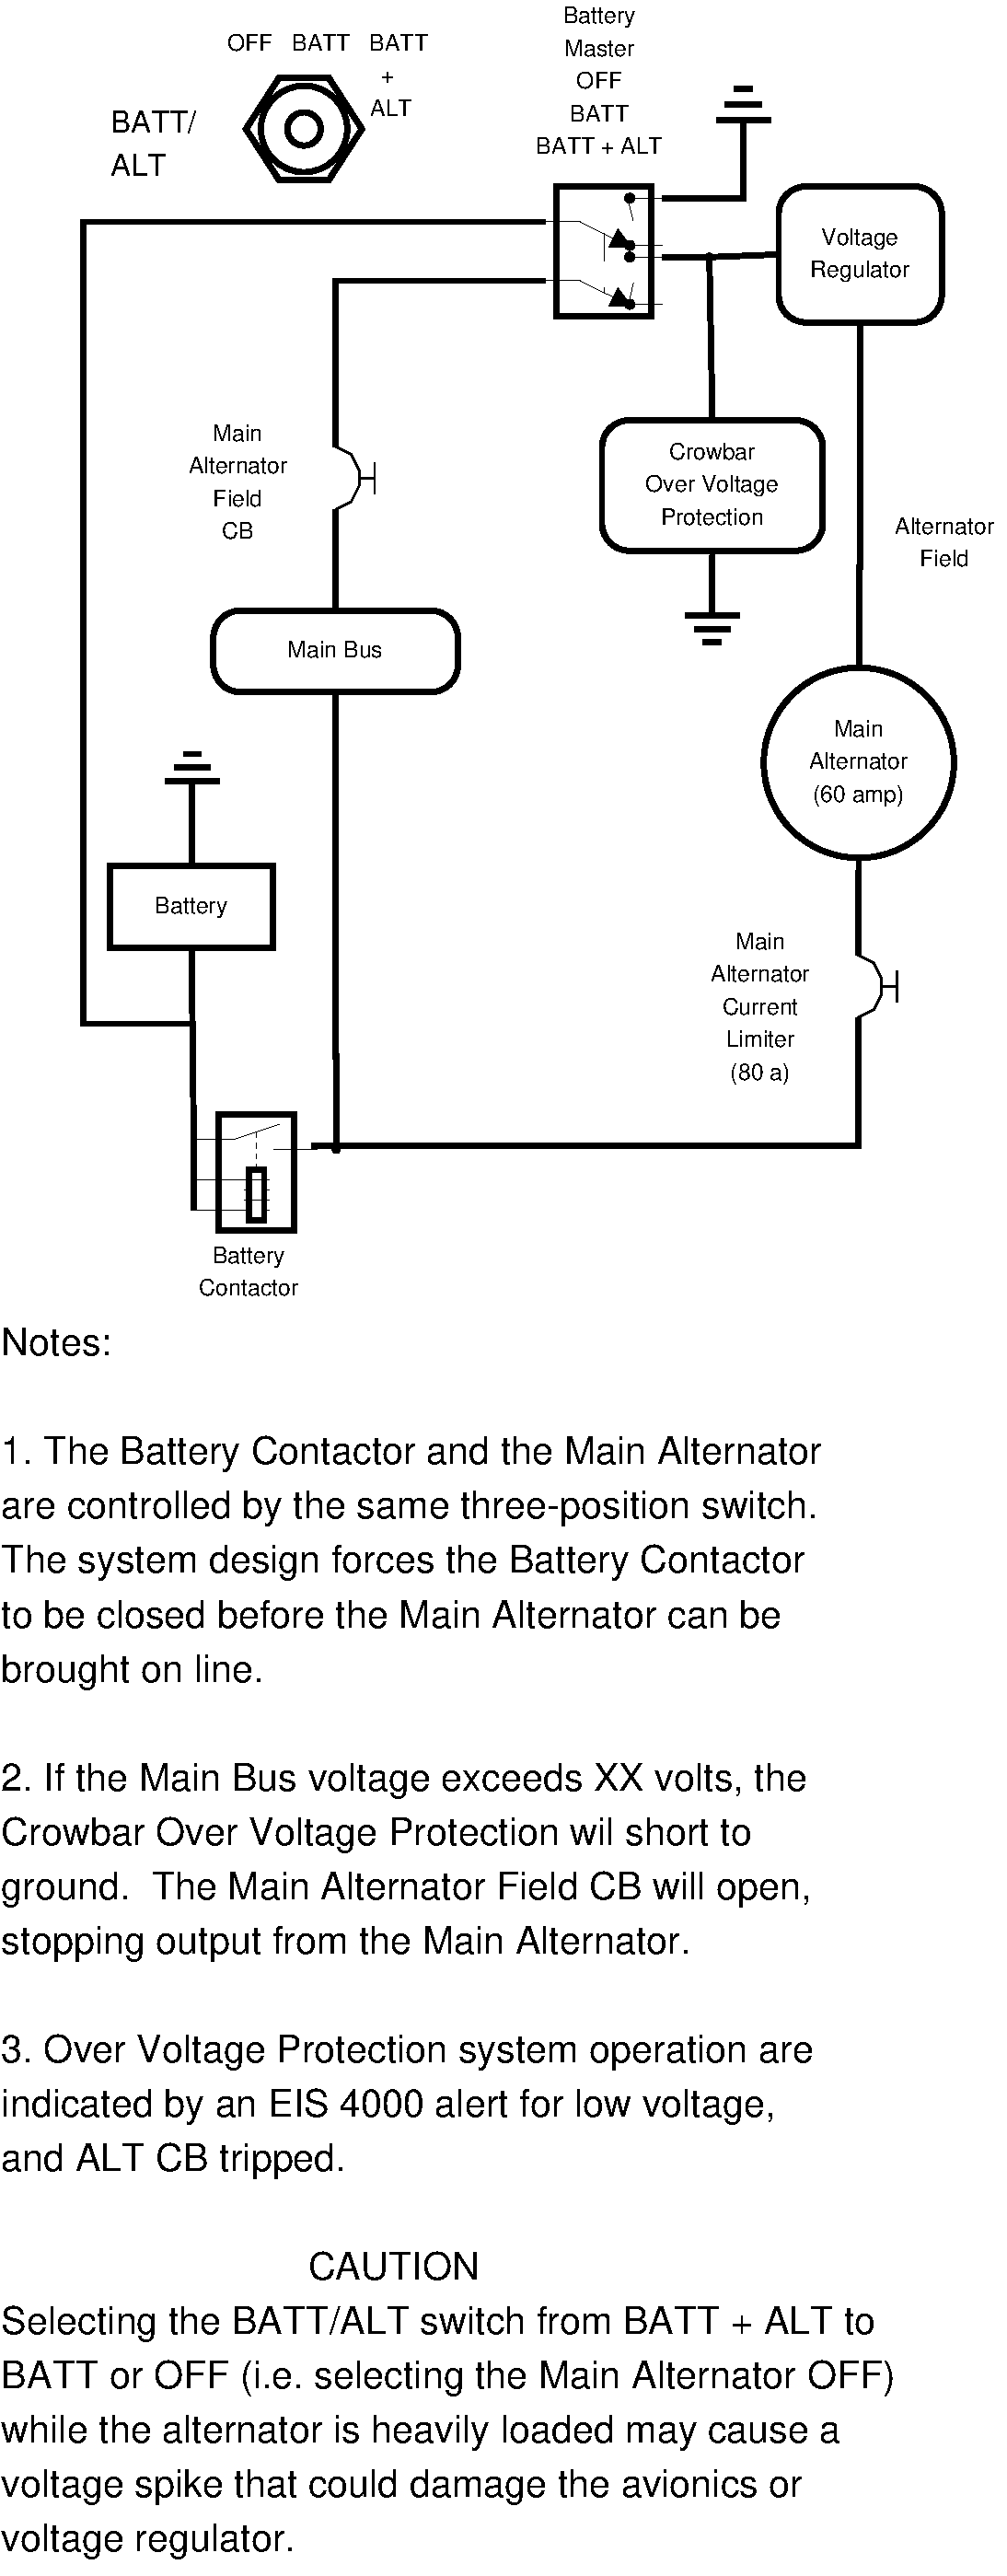
\includegraphics[scale=0.4]{../Diagrams/Alternator_large_note_narrow} \caption{Main Alternator Control} 
\end{figure}

\begin{figure}
\centering 
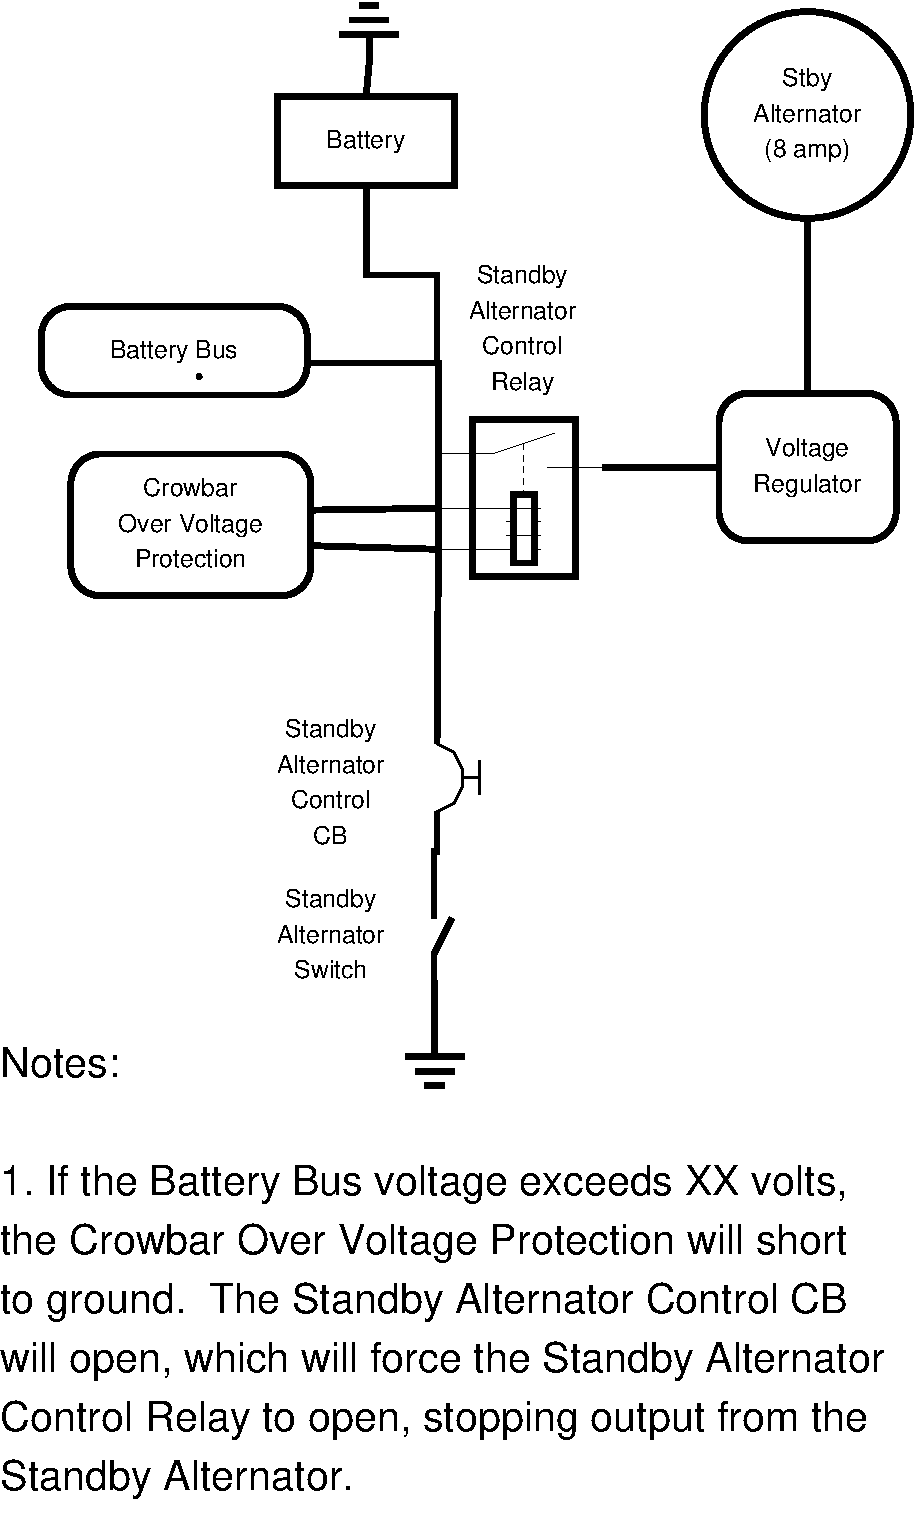
\includegraphics[scale=0.4]{../Diagrams/Alternator2_large_note_narrow} \caption{Standby Alternator Control}
\end{figure}

\textbf{Electrical System Switches} --- Electrical system switches are positioned on the right switch console. The master relay and the Main Alternator are controlled by the same three-position switch. The switch positions are OFF, BATT and BATT+ALT. The Standby Alternator can supply power to the Battery Bus, and the Essential Bus even if the BATT/ALT switch is selected to OFF.

\textbf{Over Voltage Protection} --- Each alternator has independent over voltage protection. If the alternator output voltage is too high, the over voltage protection system will short the Main Alternator field or the Standby Alternator relay to ground. This will open a CB on the aft end of the right side switch console, and shutdown the affected alternator. The over voltage protection may be reset by pushing the CB back in, but it will pop again if the over voltage condition still exists.

\textbf{Electrical System Circuit Protection} --- All circuit protection is by fuses, except for circuit breakers for the Main Alternator Field and the Standby Alternator Relay. The fuses for the Main and Essential busses are mounted on the aft face of the hinged door on the forward baggage compartment aft bulkhead, and are accessible on the ground only.  Battery Bus fuses are in a fuse block next to the battery, behind the aft baggage compartment. Fusible links are also used to protect some of the wires.

%\clearpage %force electrical system figures and table to appear, before moving on to next system
\begin{table}
[htb] 
\begin{center}
\begin{tabular}
{|l|l|l|} \hline \multicolumn{1}{|c|}{Main Bus}& \multicolumn{1}{c|}{Essential Bus} & \multicolumn{1}{c|}{Battery Bus}\tabularnewline \hline \hline EFIS Main Power & GNS 430W & Turn and Bank\tabularnewline \hline Microair COM &CDI & Electronic Ignition\tabularnewline \hline Narco 122D & Transponder & EFIS Emergency Power\tabularnewline \hline Audio Panel &Grand Rapids EIS 4000 & Aux Power Outlet\tabularnewline \hline CO Monitor &Inst. Panel Lighting & \tabularnewline \hline Engine Inst. Lighting &Goose Neck Flood Light & \tabularnewline \hline CDI Lighting &Pitch Trim & \tabularnewline \hline Landing Light &Roll Trim & \tabularnewline \hline Taxi Light &Fuel Gauges & \tabularnewline \hline Position Lights &ELT GPS Decoder & \tabularnewline \hline Strobe Lights & & \tabularnewline \hline Oil Press. Warning Light & & \tabularnewline \hline Starter & & \tabularnewline \hline Flaps & & \tabularnewline \hline Boost Pump & & \tabularnewline \hline Pitot Heat & & \tabularnewline \hline Autopilot & & \tabularnewline \hline Hour Meter & & \tabularnewline \hline Tachometer & & \tabularnewline \hline Manifold Pressure Gauge & & \tabularnewline \hline Defog Fan & & \tabularnewline \hline 
\end{tabular}
\caption{Items Powered By Each Electrical Bus} 
\end{center}
\end{table}

%\textcolor{red}{Add fuse block table}
\begin{sidewaysfigure}
\centering 
% 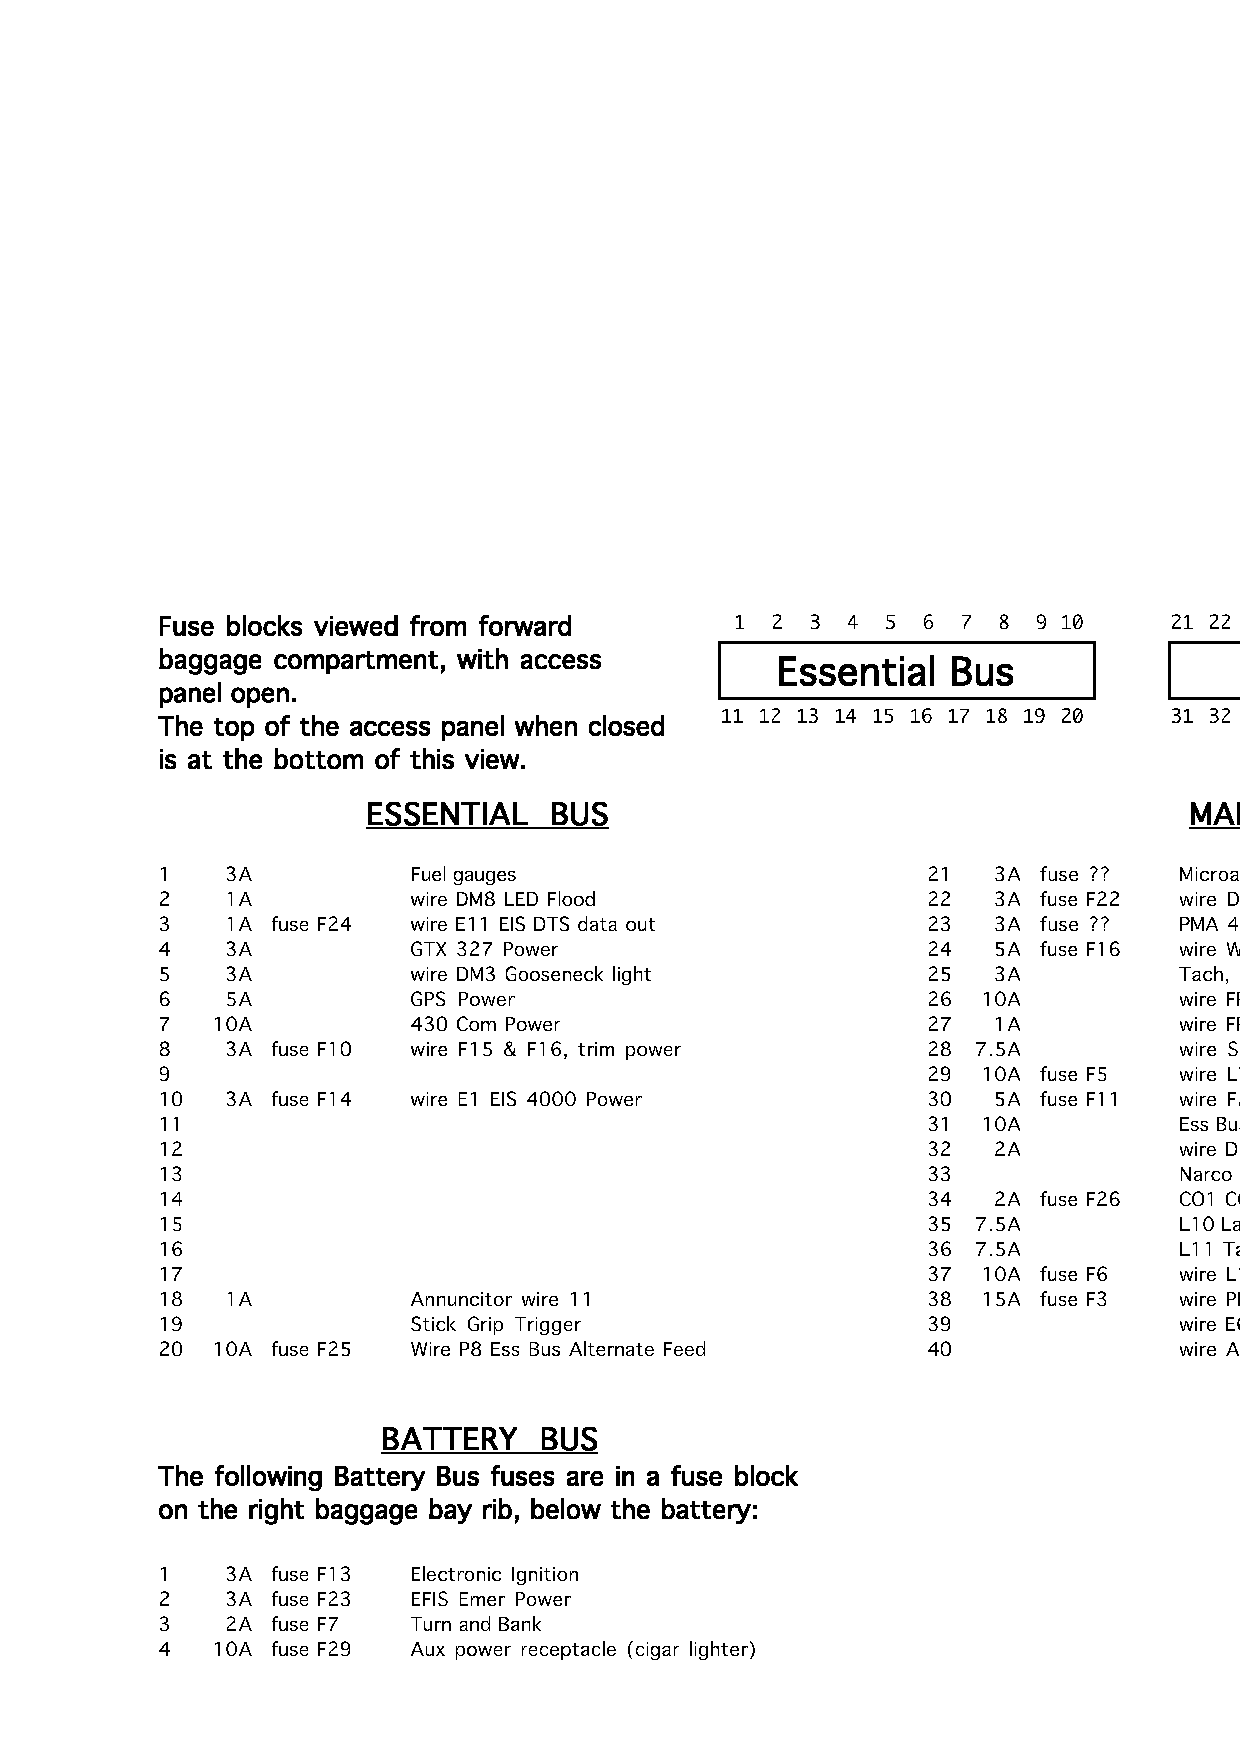
\includegraphics[width=\textwidth, scale=0.5]{../Diagrams/fuse_blocks} \caption{Fuse Locations}
% 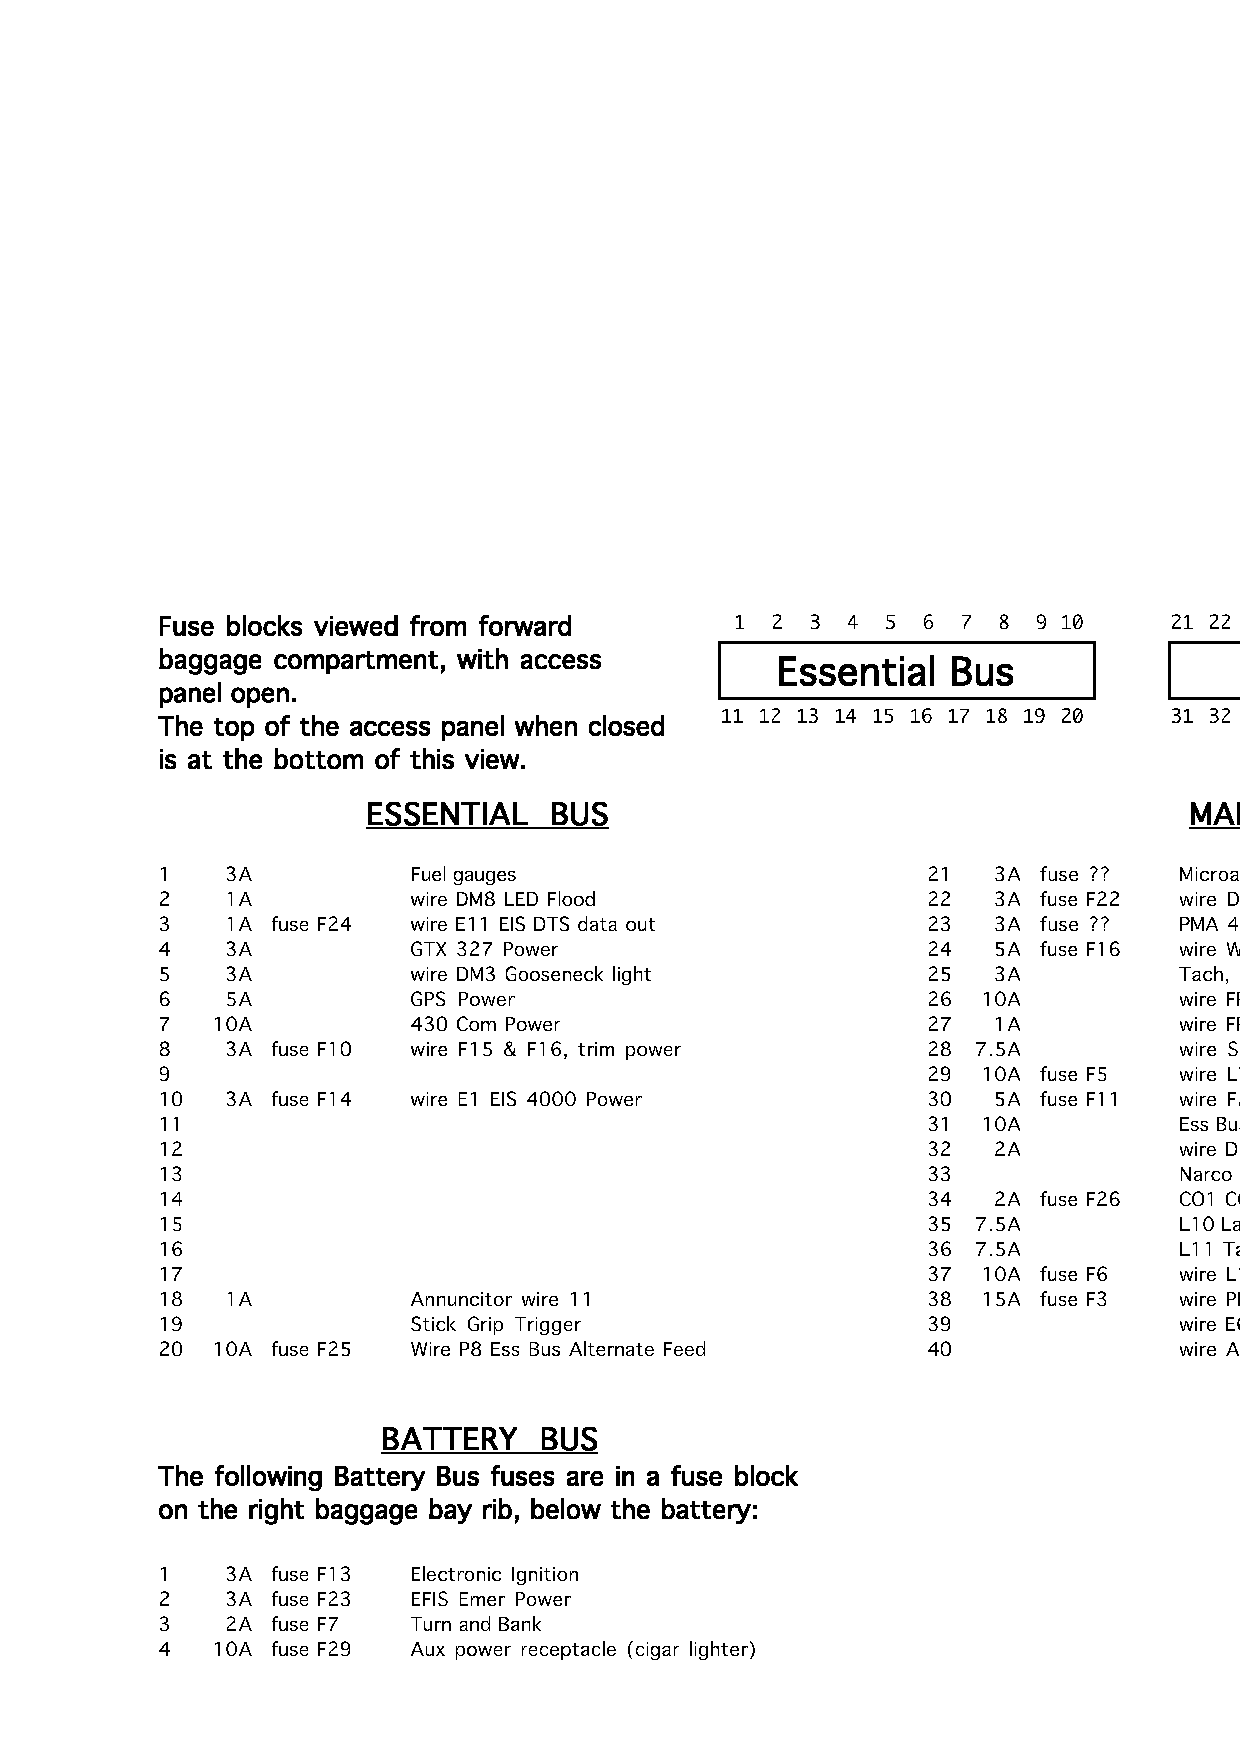
\includegraphics[scale=0.8]{../Diagrams/fuse_blocks} \caption{Fuse Locations}
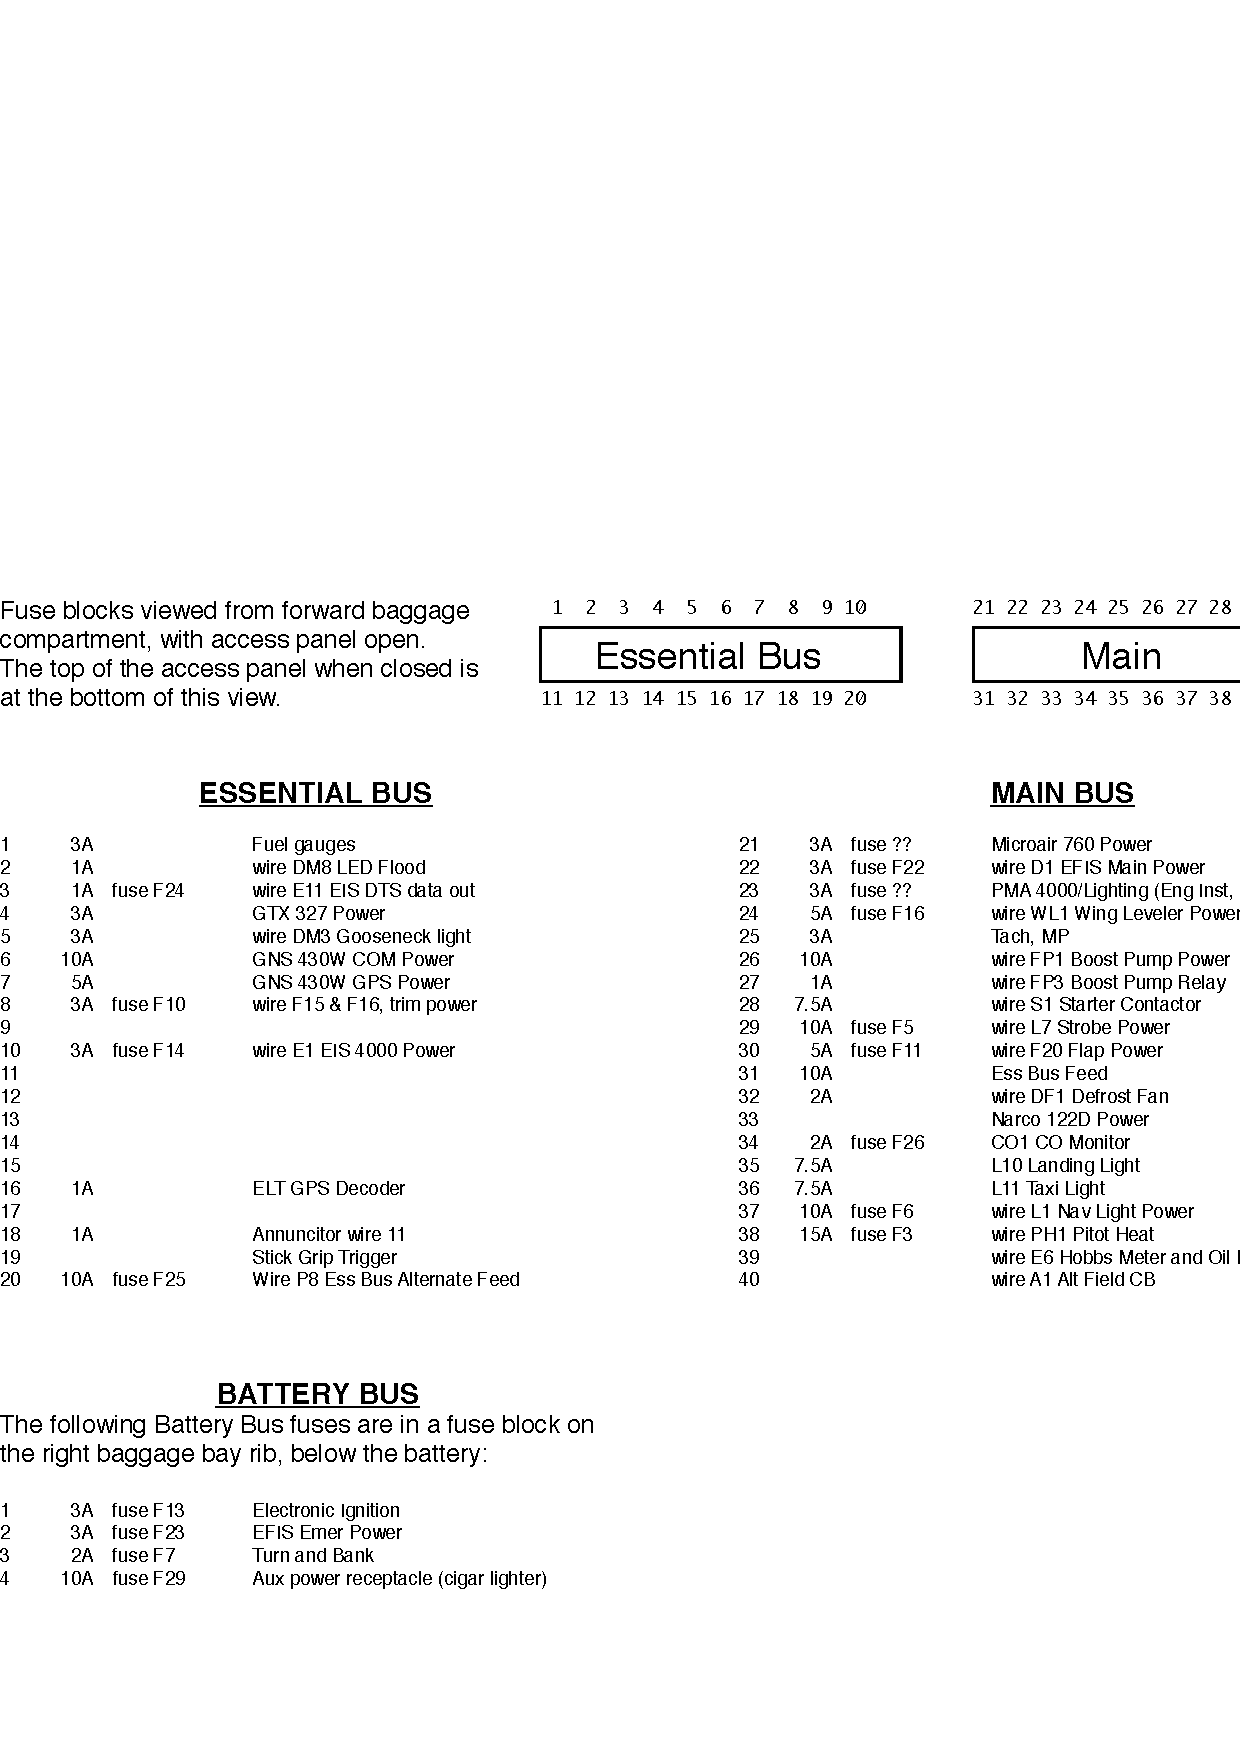
\includegraphics[scale=0.8]{../Diagrams/Fuse_Blocks_POH} \caption{Fuse Locations}


\end{sidewaysfigure}

\FloatBarrier

\section{COCKPIT LIGHTING}

\textbf{PANEL FLOOD LIGHTS} --- The main instrument panel lighting is provided by two white LED flood lights, one mounted on the front end of each canopy sill. The flood lights are powered from the Essential Bus, and are controlled by the left-most dimmer knob on the lower left part of the main instrument panel, labelled ``INST PANEL''.

\textbf{GOOSE-NECK FLOOD LIGHT} --- Map lighting and emergency instrument panel lighting is provided by a goose-neck lamp mounted on the right wall of the front cockpit, powered from the Essential Bus. It is controlled by a dimmer knob fitted next to the base of the lamp. The goose-neck may be removed from the socket by pressing the release button next to the base.

\textbf{760 COM DISPLAY} --- The display back-lighting for the Microair 760 COM is controlled by the INST PANEL dimmer knob. The display back-lighting is powered even if the 760 COM is unpowered.

\textbf{GARMIN GNS 430W \& GTX 327} --- The display and key back-lighting for the Garmin GNS 430W GPS and GTX 327 Transponder are controlled by the middle dimmer knob, labelled ``AVIONICS''. The display intensity is controlled by an ambient light sensor if the dimmer knob is rotated fully counter clock-wise --- this allows the display intensity to increase as required in bright sunlit conditions.

\textbf{ENGINE INSTRUMENTS \& CDI} --- The analog tachometer, manifold pressure, fuel gauges and CDI are internally lit --- these lights are powered from the Main Bus. The light intensity is controlled by the right-most dimmer knob, labelled ``CDI + ENG INST''. 

\section{EXTERNAL LIGHTING}

\textbf{Landing Light} --- The Landing Light is installed in the right outboard wing. It is powered from the Main Bus and uses a 55 amp halogen automotive bulb. The switch is on the left side of the instrument panel. 

\textbf{Taxi Light} --- The Taxi Light is installed in the left outboard wing, and is identical to the landing light, except it is aimed at a lower angle. It is powered from the Main Bus, and its switch is on the left side of the instrument panel.

\textbf{Flash Function} --- The Landing and Taxi Lights also have a ``wig-wag'' flash function which flashes the two lights alternately. It is selected by placing both the Landing and Taxi Light switches in the middle, ``FLASH'' position.

\textbf{Position Lights }- The aircraft is fitted with red, green and white position lights in the left wing tip, right wing tip and rudder bottom respectively. The wing tip position lights are mounted under flush covers in the forward edge of the wing tips. The rudder bottom light is in the centre of a concentric position light/strobe light assembly. The position lights are powered from the Main Bus, and the switch is located on the left side of the instrument panel. The switch has three positions: ``OFF'', ``NAV'', and ``NAV + STR''. The position lights are ON if the switch is in either of the latter two positions.

\textbf{Strobe Lights} --- The aircraft is fitted with white strobe lights, with strobe tubes under flush covers on each wing tip and on the aft end of the rudder bottom fairing. The strobe lights are powered from the Main Bus, and the switch is located on the left side of the instrument panel. The switch has three positions: ``OFF'', ``NAV'', and ``NAV + STR''. The strobe lights are ON only if the switch is in the ``NAV + STR'' positions.

\section{PITOT-STATIC SYSTEM}

The pitot system provides pitot pressure to the EFIS and the airspeed indicator. The heated pitot tube is located under the left wing, about two thirds of the way along the span. The pitot heat, powered from the Main Bus, is controlled by the PITOT HEAT switch on the right hand console.

The static system supplies static pressure to the EFIS, airspeed indicator, altimeter, vertical speed indicator and altitude encoder (which provides altitude information to the transponder). The static pressure ports are on the rear sides of the fuselage and are positioned to self drain. An alternate static port is located near the bottom of the right landing gear box in the cockpit. The alternate static port is a locking valve which is spring loaded closed. It can be pushed upwards and turned to lock it in the open position. Airspeed and altitude corrections must be applied if the alternate static port is open. 

\section{HEATING AND VENTILATION}

Cabin heat is provided via two heat muffs attached to the exhaust system and fed with high pressure air taken from the baffling behind \#3 cylinder and ahead of \#1 cylinder. The heated air is ducted through the firewall in two locations: ahead of the rudder pedals, and on the rear wall of the front baggage compartment lower extension, near the right landing gear box. The heat is controlled by two push/pull cables just below the right heat outlet. The right heat outlet is from an orientable eyeball vent that may be pointed to blow the hot air past the right side of the pilot towards the passenger.

Ventilation air is supplied from two NACA inlets: one on the front left side of the fuselage for the pilot, and one under the right wing for the passenger. The pilot's ventilation air is fed to an eyeball vent under the left side of the instrument panel. The passenger's ventilation air is fed to an eyeball vent just aft of the front seat back.

A Defog Fan is mounted beneath a grill on the glare shield. It is controlled by a switch on the right console, and blows air from under the instrument panel against the windscreen.
\clearpage 
\section{DYNON D-10A EFIS} 
\piccaption{Dynon D-10A EFIS} 
\parpic[r]{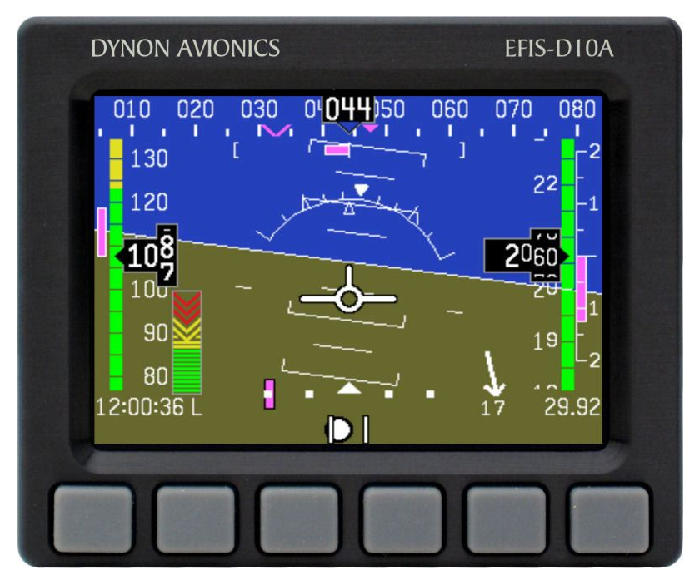
\includegraphics[scale=0.65]{../Diagrams/d10a_new_format}}

The Dynon D-10A EFIS provides attitude, heading, airspeed, altitude, vertical acceleration and slip ball information on a 4" colour LCD display.

\textbf{Operator Interface} --- The six buttons along the bottom of the bezel provide access to various functions. After a button is pushed, labels are displayed above each button. The far-right button will always command a return to the previous menu.

\textbf{Power} --- The EFIS is normally powered from the Main Bus. The unit may be turned ON by pressing the far-left button. If Main Bus power is lost, the unit will automatically transition to its internal battery for 30 seconds, then shutdown. A screen message will be displayed, warning of the impending shutdown. This automatic shutdown may be cancelled by pressing the far-left button.

If Main Bus power is lost, but aircraft battery power is still available, the EFIS BU switch on the right console may be selected to provide EFIS power from the Battery Bus.

If any power source is lost, an on-screen voltmeter display will appear, showing the voltage levels of the EFIS main power, emergency power and internal battery.

The unit may be turned OFF by pressing the holding the POWER button, which is the far-left button on the Main Menu.

\textbf{Attitude} --- The EFIS uses solid-state accelerometers and rate gyros to determine the attitude. Airspeed data is used to provide acceleration corrections, so the attitude info may be in error during manoeuvring if the pitot or static lines are blocked. The attitude information may become invalid for short periods following extreme manoeuvres (e.g. aerobatics or spins). The colours of the attitude display will be changed from the normal blue/brown to shades of grey if the EFIS detects that the displayed attitude may not be valid.

\textbf{Heading} --- The heading is sensed by a remote flux valve mounted in the rear fuselage. The flux valve may be affected by the steel canopy frame when the canopy is open. It is possible that EMI from the flux valve may be heard on the COM. The flux valve may be disabled by selecting the ``FLUX VALVE'' switch OFF on the upper left side of the instrument panel. If the flux valve is disabled, the unit will use an internal flux valve, but it has very large errors, so the heading info will be essentially meaningless.

\textbf{Altimeter Setting} --- The altimeter setting can be viewed or changed via the BARO selection from the Main Menu.

\textbf{Bugs} --- Airspeed, altitude and heading bugs may be set via the BUGS selection from the Main Menu.

\textbf{Dimmer} --- Screen intensity can be set via the DIM selection on the Main Menu 2 page {[}Main Menu $\Rightarrow$ MORE $\Rightarrow$ DIM{]}.

\textbf{Optional Display Items} --- The CLUTTR menu item allows the user to select which items are displayed {[}Main Menu $\Rightarrow$ MORE $\Rightarrow$ SETUP $\Rightarrow$ CLUTTR{]}. For example, the airspeed vertical tape and digital readouts may be independently selected, if desired. 

The INFO menu controls optional VSI, voltmeter and accelerometer displays {[}Main Menu $\Rightarrow$ MORE $\Rightarrow$ INFO $\Rightarrow$ LEFT (or RIGHT, as desired){]}.

Information on the following additional, optional functions may be found in the EFIS Pilot's User Guide:

\begin{itemize*}
\item Timer 
\item Clock 
\item G-meter 
\item VSI 
\item Turn Rate Display 
\item Checklists (not currently programmed)
\item HSI (not currently configured for display)
\end{itemize*}

\section{GARMIN GNS 430W GPS/NAV/COM} 
\begin{figure}
[htb] 
\begin{center}
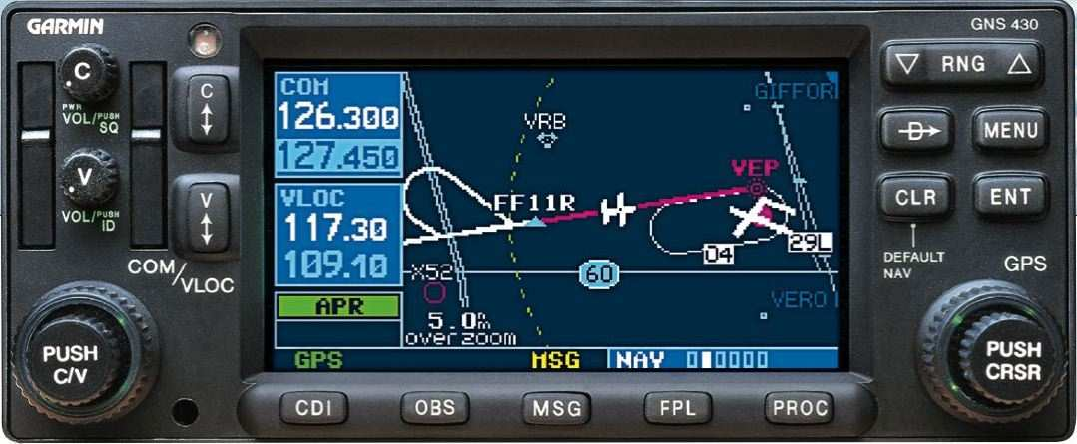
\includegraphics[scale=0.8]{../Diagrams/gns430_1}
\end{center}
\caption{Garmin GNS 430W} 
\end{figure}

This section will only provide info on basic functions required for VFR flight. See the Garmin GNS 430W Pilot's Guide and Reference for more detailed information, and coverage of IFR related functions. Some aspects of the functionality are configurable via configuration menus (see Pilot's Guide for details).

The GNS 430W System is a fully integrated, panel mounted instrument, which contains a VHF Communications Transceiver, a VOR/ILS receiver, and a Wide Area Augmentation System (WAAS) Global Positioning System (GPS) Navigation computer. The system consists of a GPS antenna, GPS Receiver, VHF VOR/LOC/GS antenna, VOR/ILS receiver, VHF COMM antenna and a VHF Communications Transceiver. 

Provided the Garmin GNS 430W's GPS receiver is receiving adequate usable signals, it has been demonstrated capable of and has been shown to meet the accuracy specifications for:
\begin{enumerate}
\item VFR/IFR enroute, terminal, and non-precision instrument approach (GPS, VOR, VOR-DME, NDB, NDB-DME, RNAV) operation using WGS-84 (or NAD 83) coordinate reference datum in accordance with AC 20-138. \textcolor{red}{Add WAAS info.}
\item The system meets RNP5 airspace (BRNAV) requirements of AC 90-96 and in accordance with AC 20-138, and JAA GAI-20 ACJ 20X4, provided it is receiving usable navigation information from the GPS receiver. 
\item The equipment as installed has been found to comply with the requirements for GPS primary means of navigation in oceanic and remote airspace, when used in conjunction with the 400 Series Trainer Program incorporating the FDE Prediction Program. This does not constitute an operational approval. 
\end{enumerate}
Navigation is accomplished using the WGS-84 (NAD-83) coordinate reference datum. Navigation data is based upon use of only the Global Positioning System (GPS) operated by the United States of America.

The GNS 430W provides GPS, COM, VOR, LOC and G/S capability with a colour moving map display. The COM is connected to the COM 1 on the audio panel. The CDI may display either GPS, VOR or ILS info.

\textbf{Power} --- The GNS 430W is powered from the Essential Bus. The unit is turned ON/OFF by turning the COM PWR/VOL switch at the top left corner. The Self-Test page data must be verified for IFR navigation using the GPS.

\textbf{COM} --- The GNS 430W COM is connected to the COM1 selection of the Audio Panel. The COM volume is controlled by the PWR/VOL knob at the top left corner. This knob is pushed to toggle the squelch ON/OFF. Two concentric tuning knobs at the lower left select the standby frequency for the COM and NAV. The frequency tuning function will default to COM, but it may be toggled between the COM and NAV functions by pushing the inner tuning knob (marked ``PUSH C/V''). The standby and active frequencies are exchanged by pushing the ``C$\updownarrow$'' button.  Press and hold the ``C$\updownarrow$'' button to switch to 121.5 mHz.

\textbf{NAV} --- The frequencies are tuned as described in the COM section. The NAV audio may be selected via the audio panel. The NAV volume is controlled by the lower of the two VOL knobs (marked ``V''). The NAV idents are not fed to the NAV audio by default, but they may be selected by pushing the NAV volume knob.

\textbf{CDI} --- the external CDI nav source is selected to either GPS or NAV by the CDI button on the bottom bezel. The current CDI nav source is indicated above the CDI button and by a lit indication on the CDI itself. If GPS is the nav source, the CDI scaling is indicated above the CDI button (see Table \ref{cdi} below).

\begin{Note}
\centering
The internal CDI display on the NAV 1 page always shows GPS information.
\end{Note}
\raggedright

\begin{table}
[htb] 
\begin{center}
\begin{tabularx}
  % {\textwidth}{|>{\setlength\hsize{.5\hsize}}Y|c|>{\setlength\hsize{1.5\hsize}}Y|} \hline Annunciation&Meaning\\
  {\textwidth}{|c|X|c|} 
  \hline ANNUNCIATION&MEANING&APPROACH\tabularnewline
  &&MINIMUMS\\
	\hline
	\hline DPRT & Departure, indicates the system is using non- precision approach integrity. HAL = 0.3 and CDI full-scale deflection is 0.3 NM.&\\
	\hline ENR & En route, CDI full-scale deflection is 2.0 NM or current CDI scale selection, whichever is smaller.&\\
	\hline TERM & Terminal, CDI full-scale deflection is 1.0 NM or current CDI scale selection, whichever is smaller.&\\
	\hline LNAV & GPS approach active. &LNAV\\
	\hline LNAV+V & GPS approach active + advisory baro vertical guidance.&LNAV\\
	\hline L/VNAV & Lateral Navigation and Baro Vertical Navigation (LNAV/VNAV) approach active. &LNAV/VNAV\\
	\hline LP & LP indicates Localizer Performance active with no vertical guidance.&LP\\
	\hline LPV & Localizer Performance with Vertical guidance (LPV) approach active.	A yellow background indicates that the approach is safe to continue but a downgrade to LNAV may occur.&LPV\\
	\hline MAPR & Missed Approach indicates the system is providing missed approach integrity and CDI full-scale deflection $\pm $0.3 NM.&\\
  \hline LOW ALT & For LNAV+V, LNAV/VNAV, or LPV approaches, the LOW ALT annunciation indicates the aircraft's estimated height is significantly lower than the Final Approach Waypoint height.&\\
	\hline
\end{tabularx}
\caption{CDI Scaling Indications} \label{cdi}
\end{center}
\end{table}

\textbf{GPS Direct-To} --- For GPS Direct-To navigation, push the \directto button. Dial up the identifier using the inner right knob to select characters, and the outer right knob to move to the next character. Press ENT when the identifier is complete. Press ENT again to activate.

\textbf{Colour Moving Map Display} --- Press the CLR button to go to the default NAV page (CDI type display plus digital nav data). Rotate the inner right knob one click to the right to get to the moving map display. The range is changed with the Range rocker switch at the top right of the unit.

\textbf{Nearest Airports} --- Rotate the right outer knob all the way to the right, to display the NRST pages. Rotate the inner right knob all the way to the left to the Nearest Airports page. The three nearest airports are displayed, with six additional near airports available if the page is scrolled. The page may be scrolled by pushing the right inner knob to enable the cursor, then rotating the right inner knob to move the cursor. Direct-to navigation may be selected to an airport by moving the cursor to the airport identifier, then pressing the \directto button.

The airport tower or traffic frequency may be moved to the COM standby position by moving the cursor to the desired frequency on the NRST page and pressing the ENT button. Press the ``C$\updownarrow$'' button to exchange the standby and active COM frequencies.

\textbf{Antennae} --- The GPS/WAAS antenna is mounted on the upper fuselage immediately behind the passenger seat. The COM antenna is mounted on the left side of the bottom of the fuselage just behind the wing main spar. The NAV antenna is mounted inside the right wing tip. The signal from the NAV antenna also provides glide slope info.

\section{MICROAIR 760 COM} 
\piccaption{Microair 760 COM} 
\parpic[r]{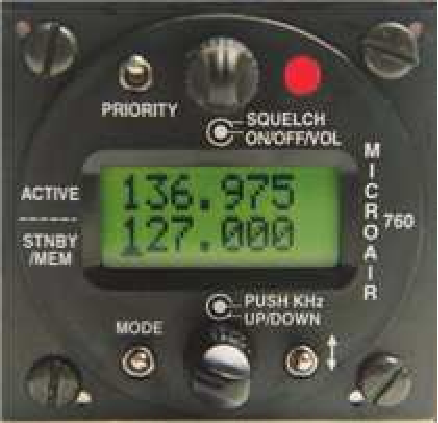
\includegraphics[scale=0.842]{../Diagrams/microair}}


The Microair 760 COM radio is positioned in a 2 1/8" instrument hole on the upper left side of the instrument panel above the GNS 430W, and is connected to the COM2 position of the Audio Panel.

\subsection*{Controls and Indicators}

\textbf{PRIORITY} --- Top left. A momentary down push selects the frequency in Memory 25, which is 121.5 MHz by default.

\textbf{ON/OFF/VOL} --- Inner top knob. Controls power and volume. 

\textbf{SQUELCH} --- Outer top knob.

\textbf{Annunciator LED} --- Top right. Indicates:

\begin{tabular}{lp{2.9in}} 
Red (steady)&Radio is transmitting\\
Red (flashing)&Radio has transmitted for longer than 30 seconds.\\
Green&A signal is received, or the squelch is set so background static is heard.\\
Off&Radio is not receiving a signal, and the squelch is set so background static is not heard.\\
\end{tabular}

\textbf{MODE} --- Bottom left. Momentary down pushes on the Mode toggle cycle the 760 COM thru the four modes of frequency selection. 
\begin{enumerate}
\item \textbf{Flip-Flop Mode} --- Flip-Flop mode has an active/standby functionality, with the active frequency displayed above the standby one. The standby frequency is changed using the bottom knob. Push the knob momentarily to switch the control between MHz and KHz. The control defaults to MHz after five seconds of inactivity. An underline cursor indicates the field that is currently selected. The active and standby frequencies are exchanged by making a momentary down movement on the $\updownarrow$ toggle. 
\item \textbf{Memory Mode} --- The top line displays ``MEM XX'', where ``XX'' is the memory number. The lower line displays the frequency in that memory location. The available frequencies are scrolled by rotating the frequency knob (lower knob). A frequency becomes active the moment it is displayed. 
\item \textbf{Program Mode} --- Used to program the frequencies stored in the current memory location. The top line displays ``PROG XX'', where ``XX'' is the memory number. The frequencies in each memory location may be changed. Lower knob changes frequency and memory number (momentary press of knob cycles it between MEM, MHz and KHz). The frequency is stored by a momentary press of the $\updownarrow$ toggle. The memory location is cleared by pressing and holding the Priority switch 
\item \textbf{Scan Mode} --- Scan mode is selected by pressing and holding the Priority toggle for three seconds. The radio cycles through the memory frequencies, stopping for 10 seconds on each frequency that has a signal. Scan operation is terminated by a momentary press of the $\updownarrow$ toggle, or the PTT switch. 
%\item \textbf{Priority Switch} --- A momentary down push on the Priority toggle selects the frequency in Memory 25, which is 121.5 MHz by default. 
\end{enumerate}

\subsection*{Other}

\textbf{Power Source} --- The 760 COM is powered from the Main Bus.

\textbf{Back-lighting} --- The display back-lighting intensity is controlled by the \textcolor{red}{INST PANEL} dimmer.

\textbf{Antenna} --- The 760 COM is connected to an antenna inside the left wing tip. 

\section{NARCO 122D VOR/ILS}
\piccaption{Narco 122D} 
\parpic[r]{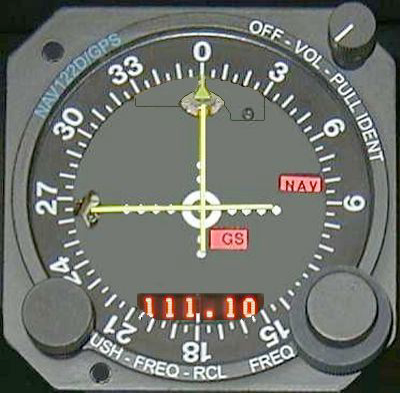
\includegraphics[scale=0.92]{../Diagrams/Narco122D_large}}


The Narco 122D is a VOR/ILS receiver with an integral CDI display. It is located at the lower, centre part of the instrument panel, directly below the CDI. The Narco 122D is \textbf{not} connected to the audio panel, so it is not possible to listen to navaid idents. 

\subsection*{Controls and Indicators}

\textbf{OFF --- VOL --- PULL IDENT} --- Top right. Controls power. The 122D is not connected to the audio panel, so the VOL and PULL IDENT functions are inoperative.

\textbf{FREQ} --- Bottom right. Inner and outer concentric knobs to select the VOR or ILS frequency.

\textbf{Course Select} --- Unlabelled knob at bottom left. Selects the desired course.

\subsection*{Other}

\textbf{Power Source} --- The Narco 122D is powered from the Main Bus. 

\textbf{Back-lighting} --- The Narco 122D has no internal backlighting.  It is illuminated by the instrument panel flood flights.

\textbf{Antenna} --- The Narco 122D receives NAV and G/S signals from the same antenna that feeds the GNS 430W, which is mounted inside the right wing tip.

\clearpage 
\section{AUDIO PANEL} 
\piccaption{PMA-4000 Audio Panel} 
\parpic[r]{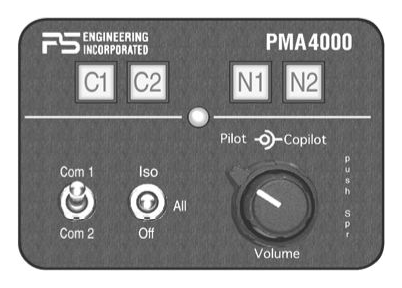
\includegraphics[scale=1]{../Diagrams/pma4000}}

The PS Engineering PMA-4000 Audio Panel is located at the bottom of the avionics stack on the left side of the instrument panel.

\subsection*{Controls}

\textbf{Audio Selector Switches} --- Top. The four square audio selector switch are labelled as follows: 
\begin{itemize}
\item ``C1'' COM 1 --- GNS 430W COM 
\item ``C2'' COM 2 --- Microair 760 COM 
\item ``N1'' NAV 1 --- GNS 430W NAV audio 
\item ``N2'' NAV 2 --- not used. 
\end{itemize}

The switches are lit when selected (pressed in). The COM that is selected for transmission is also automatically selected for audio. Both the pilot and passenger may transmit. Only the person who pushes the PTT is heard on the transmission.

\textbf{Transmit Selector} --- Bottom left. The COM radio to be used for transmission is selected by the ``Com 1/Com 2'' toggle switch.

\textbf{Mode Selector} --- Bottom centre. The audio panel mode of operation is selected with the ``Iso/All/Off'' toggle. The modes work as follows: 
\begin{itemize}
\item \textbf{Iso} --- Pilot is isolated from the intercom and music audio. The pilot only hears the Com audio (and transmission side tone). The passenger hears only himself on the intercom and the music. 
\item \textbf{All} --- Both pilot and passenger hear intercom, radios and music. The music is automatically muted when the intercom is used. 
\item \textbf{Off} --- The audio power is not powered. The pilot is automatically directly connected to Com 1 transmission and reception, regardless of the switch selections. 
\end{itemize}

\textbf{Volume} --- Bottom right. The pilot's audio volume is controlled by the inner knob, labelled ``Pilot''. The passenger's volume is controlled by the outer knob, labelled ``Copilot''. \textcolor{red}{Headset volume controls too?}

\textbf{Squelch} --- There is no dedicated Squelch control. The audio panel processor continuously adjusts the squelch as required.

\textbf{PTT} --- The pilot's PTT is the black switch half-way up the left side of the stick grip. The rear seat PTT is the black button next to the headset jacks on the right cockpit side under the canopy sill.

\textbf{Hot Mike} --- Both pilot and passenger intercom are always in a ``hot mike'' configuration. 

\section{GARMIN GTX 327 TRANSPONDER}

The Garmin GTX 327 transponder is located below the GNS 430 on the left side of the instrument panel. It is supplied with pressure altitude data by an ACK A-30 altitude encoder. Some aspects of the functionality are configurable via configuration menus (see Pilot's Guide for details).
\begin{figure}
[htb] 
\begin{center}
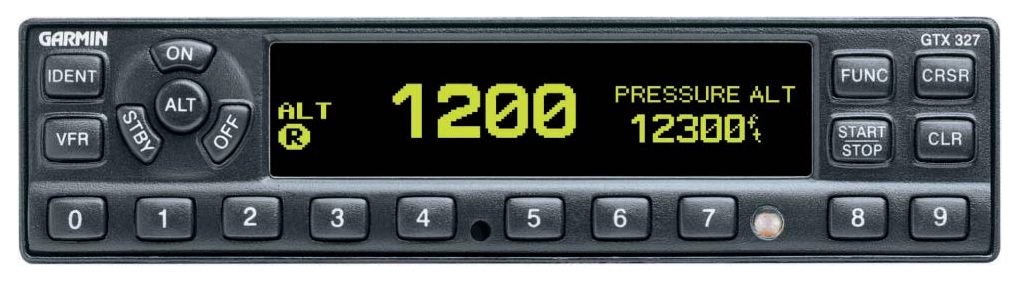
\includegraphics[scale=0.8]{../Diagrams/GTX327}
\end{center}
\caption{Garmin GTX-327 Transponder} 
\end{figure}

\subsection*{Controls}

\textbf{ON} --- Selects Mode A. Transponder replies to interrogations, but does not report altitude.

\textbf{OFF} --- Turns off the transponder.

\textbf{STBY} --- Puts the transponder in standby mode. The altitude encoder is powered and starts warming up. 

\textbf{ALT} --- Selects Mode A and Mode C. Transponder responds to interrogations and reports altitude, if the altitude encoder has warmed up. The altitude encoder requires approximately seven minutes of power to warm up. 
%The transponder automatically switches from standby to ALT mode after takeoff, based on a ground speed signal from the GNS 430.

\textbf{IDENT} --- Sends an Ident pulse to the ground station for 18 seconds.

\textbf{VFR} --- Changes the code to 1200. Pressing VFR a second time returns the code to the previous value.

\textbf{0--7} --- Used to enter a new transponder code. Code selection is started by pressing a digit. The new code will not be activated until the fourth digit is entered. Pressing the CLR key will move the cursor back to the previous digit. Pressing the CRSR key will cancel code entry and return to the previous code.

\textbf{8--9} --- Used in Configuration Mode or to set the timer.

\textbf{FUNC} --- Changes the data shown on the right side of the display. Options are Pressure Altitude, Flight Time, Count-Up Timer, Count-Down Timer, Contrast and Display brightness. Note: the availability of Contrast and Brightness selections are controlled by a configuration menu.

\textbf{CRSR} --- Used to cancel code entry, and to enable the cursor to input the time for a Count-Down timer.

\textbf{$\mathrm{\frac{START}{STOP}}$} --- Starts and stops the count-up and count-down timers.

\textbf{CLR} --- Resets the count-up and count-down timers and cancels a key press during code entry.

\subsection*{Timers}

\textbf{Count-Up Timer} --- To operate the Count-Up Timer: 
\begin{enumerate}
\item Press the ``FUNC'' key until ``COUNT UP'' is displayed. 
\item If necessary, press ``CLR'' to reset the timer to zero. 
\item Press $\mathrm{\frac{START}{STOP}}$ to start the timer. 
\item Press $\mathrm{\frac{START}{STOP}}$ again to pause the timer. 
\item Press ``CLR'' to reset the timer to zero. 
\end{enumerate}

\textbf{Count-Down Timer} --- To operate the Count-Down Timer: 
\begin{enumerate}
\item Press the ``FUNC'' key until ``COUNT DOWN'' is displayed. 
\item Press the ``CRSR'' key and use the ``0--9'' keys to set the initial time. All digits must be entered, including leading zeros. 
\item Press $\mathrm{\frac{START}{STOP}}$ to start the timer counting down. 
\item Press $\mathrm{\frac{START}{STOP}}$ again to pause the timer. 
\item When the timer expires, the words ``COUNT DOWN'' are replaced with ``EXPIRED'', and the timer begins counting up and flashing. 
\item Press ``CLR'' to reset the timer to the initial value. 
\end{enumerate}

\subsection*{Other}

\textbf{Power Source} --- The GTX 327 transponder is powered from the Essential Bus.

\textbf{Back-lighting} --- The display back-lighting intensity is controlled by the Avionics dimmer.

\textbf{Antenna} --- The GTX 327 transponder antenna antenna is mounted on the right side of the bottom of the fuselage just behind the wing main spar. 

\FloatBarrier 

%\section{WING LEVELER} 

The Navaid Devices AP-1 Wing Leveler may be operated in Turn Coordinator mode or Wing Leveler mode. A horizontal red LED display indicates turn rate. In Wing Leveler mode, wing leveler and GPS tracking modes are available. The WING LVLR switch on the LH console controls power to the wing leveler system. The power to the servo may be temporarily interrupted by pressing and holding the red master disconnect switch on the pilot's control stick. There is a clutch in the system that will slip to allow the pilot to override the wing leveler if required. %As a last resort, there is a removable pin where the wing leveler push rod connects to the base of the pilot's control stick. 

\subsection*{Controls}
\begin{tabular}{p{0.5\linewidth}p{0.5\linewidth}}
\begin{minipage}[b]{\linewidth}
\begin{enumerate}
\item \textbf{TK$\bullet$TC$\bullet$WL} --- Selects the mode of operation --- Track (TK), Turn Coordinator (TC), or Wing Leveler (WL). In Track mode, the unit tracks the GPS or NAV/LOC signal from the GNS 430, whichever is selected as the GNS 430W CDI source. In Turn Coordinator Mode, the unit is not connected to the flight controls, and simply serves as a back-up Turn Coordinator. In Wing Leveler mode, the unit provides aileron inputs to maintain zero yaw rate, or to turn, as controlled by the Turn knob. 
\item \textbf{TRIM} --- Adjusts the reference from the built-in yaw gyro. Used if the wings are not level when the Turn knob is in the centre detent. 
\item \textbf{TURN} --- Commands turns when the unit is in Wing Leveler mode. 
\item \textbf{TRIM POTS} --- Used to set the gains during flight testing. Should not be adjusted except as part of a dedicated flight test program. 
\end{enumerate}
\end{minipage} 
&
\begin{minipage}[b]{\linewidth}
\begin{overpic}
[scale=.8]{../Diagrams/ap1} 
\Large 
\put(7,36){\ding{172}} 
\put(7,52.5){\ding{173}} 
\put(95.5,52.5){\ding{174}} 
\put(95.5,28.75){\ding{175}} 
\put(-1,59.75){\ding{176}} 
\put(79,81.25){\ding{177}} 
\put(82,.75){\ding{178}} 
\normalsize 
\end{overpic}
\caption{Wing Leveler}
\end{minipage}\\
\end{tabular}

\subsection*{Indicators} 
\begin{enumerate}
\setcounter{enumi}{4} 
\item \textbf{TURN RATE} --- Bar of red LEDs illuminate to indicate turn rate. The centre LED is illuminated at zero turn rate. The bar extends from the centre to indicate the magnitude and direction of the turn rate. 
\item \textbf{STANDARD TURN MARKERS} --- Triangles above the turn rate bar indicate a 3 deg/second turn rate. 
\item \textbf{SLIP BALL} --- Indicates lateral acceleration. 
\end{enumerate}

\subsection*{Power}

\textbf{MAIN POWER} --- The Wing Leveler power is controlled by the WING LVLR switch on the right switch console. The unit is powered from the Main Bus.

\textbf{SERVO DISENGAGE} --- The servo power supply may be interrupted by pressing and holding the red TRIM/WING LEVELER disable switch on the front stick grip. %If required, the linkage between the servo and the stick may be disconnected by pulling the ``Pip'' pin that is located at the bottom of the front stick, just above the fore and aft pivot.



\section{AUTOPILOT} 

The Trio Avionics Pro Pilot autopilot moves the ailerons and/or elevators to control the aircraft. The autopilot can follow the GNS 430W lateral flight plan, including procedure turns and GPS, RNAV or LPV approaches. The autopilot vertical capabilities include altitude hold, vertical speed hold, altitude preselect and LPV vertical path. A two line alphanumeric display provides detailed information to the pilot. The WING LVLR switch on the LH console controls power to the autopilot system. The power to the servos may be temporarily interrupted by pressing and holding the red master disconnect switch on the pilot's control stick. The autopilot does not control the pitch trim --- the aircraft must be reasonably well trimmed in pitch to allow the autopilot to control the aircraft without reaching the force limit provided by the servo slip clutch. %Each servo has a clutch that will slip to allow the pilot to override the wing leveler if required. %As a last resort, there is a removable pin where the wing leveler push rod connects to the base of the pilot's control stick. 

The autopilot control head is on the instrument panel below the turn and slip indicator. The pitch servo is behind the rear baggage compartment, and the roll servo is beneath the horizontal panel just ahead and to the right of the front seat. The autopilot is powered from the Main Bus. Power is controlled by the Wing Leveler switch on the right console and also by the On toggle switch located at the top centre of the control head.

\textbf{Altimeter Setting} --- The autopilot does not have a means to directly enter an altimeter setting. Instead, the current altitude is entered whenever the "BARO SET" message is displayed, which allows the system to determine the needed offset to the pressure altitude sensed from the static input.

\subsection*{Controls}
\begin{tabular}{p{0.5\linewidth}p{0.5\linewidth}}
\begin{minipage}[b]{\linewidth}
\begin{enumerate}
\item \textbf{Power Switch} --- Controls all power to the autopilot control head and servos. This switch is in series with the Wing Leveler switch on the right switch console.
\item \textbf{"H~NAV"} --- Engages or disengages the horizontal (i.e. roll) servo. A three second press and hold engages the autopilot in emergency left course reversal (180\textdegree \ left turn with altitude hold).
\item \textbf{"V~NAV"} --- Engages or disengages the vertical (i.e. pitch) servo. A three second press and hold engages the autopilot in emergency right course reversal (180\textdegree \ right turn with altitude hold).
\item \textbf{"H~MODE"} --- Cycles the horizontal mode between TRK (track), CRS (course) and INT (intercept) modes, if the display is currently showing horizontal mode info. If the autopilot display is currently showing vertical mode information, the first press of the "H~MODE" button replaces that with horizontal mode information.
\item \textbf{"V~MODE"} --- Cycles the vertical mode between ALT HOLD (altitude hold), AS/VS (airspeed/vertical speed), ALT SEL (altitude select) and BARO SET (adjust altitude for altimeter setting changes). If the autopilot display is currently showing horizontal mode information, the first press of the "H~MODE" buttons replaces that with vertical mode informational.
\item \textbf{Rotary Knob} --- Allows pilot input of values by rotation and then pushing to enter. For changes to selected altitude, one click = 100 ft. If the knob is pressed, then turned, one click = 1000 ft. For changes to selected track, one click = 1\textdegree.
\end{enumerate}
\end{minipage} 
&
\begin{minipage}[b]{\linewidth}
\begin{overpic}
[scale=.8]{../Diagrams/ProPilot5} 
\end{overpic}
\caption{Trio Pro Pilot Autopilot}
\end{minipage}\\
\end{tabular}

\subsection*{Indicators} 
\begin{enumerate}
\setcounter{enumi}{6} 
\item \textbf{H LED} --- Illuminates when the horizontal servo is engaged. 
\item \textbf{V LED} --- Illuminates when the vertical servo is engaged. 
\item \textbf{GPSS LED} --- Blinks when roll steering info from the GNS 430W is available, but not being used because the autopilot is not in TRK mode. Illuminates steady when the autopilot is following roll steering info from the GNS 430W. The autopilot must be in TRK mode to use GPSS.
\item\textbf{GPSV LED} --- Blinks when vertical steering info from the GNS 430W is available, but not being used because the autopilot is not in TRK mode. Illuminates steady when the autopilot is using vertical steering info from the GNS 430W. GPSV info is only available when the GNS 430W is currently on an instrument approach with vertical guidance (LPV, L/VNAV or LNAV+V).
\item \textbf{H MODE LEDs} --- TRK, CRS and INT LEDs illuminate steady or flashing to indicate current horizontal mode.
\item \textbf{V MODE LEDs} --- ALT HLD, AS/VS and ALT SEL LEDs illuminate steady or flashing to indicate current vertical mode.
\item \textbf{SLIP BALL} --- Indicates lateral acceleration. 
\item \textbf{H/V FUNCTION ARROW} --- Indicates whether the right side of the display and rotary knob are dedicated to H~MODE (arrow pointing left) or V~MODE functions (arrow pointing right). If the arrow is pointing left, a single press of the V~MODE button will switch the arrow to the right. Subsequent presses of the V~MODE button will change the vertical mode. Similarly, if the arrow is pointing to the right, a single press of the H~MODE button will switch the arrow to the left.
\end{enumerate}

\subsection*{Power}

\textbf{MAIN POWER} --- The unit is powered from the Main Bus. The toggle switch at the top centre of the control head is in series with the WING LVLR switch on the right console.

\subsection*{Engagement and Disengagement}

\textbf{SERVO ENGAGEMENT} --- The pitch and roll servos are engaged individually by pressing and releasing the "V~NAV" and "H~NAV" buttons at the top of the control head. The green "V" and "H" LEDs illuminate when the vertical (i.e. pitch) and horizontal (i.e. roll) servos are engaged. The default horizontal and vertical modes are TRK and ALT HLD.

\textbf{SERVO DISENGAGEMENT} --- The autopilot may be disengaged by a quick press and release (press and release within 5 seconds) of the red TRIM/AP disable switch on the front stick grip. The pitch and roll servos may be individually disengaged by pressing and releasing the "V~NAV" and "H~NAV" buttons respectively. %If required, the linkage between the servo and the stick may be disconnected by pulling the ``Pip'' pin that is located at the bottom of the front stick, just above the fore and aft pivot.

\subsection*{H~NAV Modes}
The following horizontal modes are available:

\textbf{TRK} --- Track mode uses roll inputs to follow a GPS flight plan or Direct-To. GPS Steering (GPSS) data will be used if available, in which case the roll steering commands are coming from the GNS 430W. TRK is the default power-up mode, if a GPS flight plan or Direct-To is available.

\textbf{CRS} --- Course mode uses roll inputs to fly a selected GPS course angle (i.e. a selected track with respect to magnetic north). The selected course is seen on the top left of the display, labelled "CRS". The selected course is adjusted by turning the rotary knob, if the H/V function arrow (middle of the top line) is pointing to the left. The actual track is shown just below, labelled "TRK". CRS is the default power-up mode if GPS data is available but no flight plan or Direct-To has been entered.

\begin{Note}
ATC often requests a specific heading to be flown. CRS mode allow a specific track to be flown. The CRS can be changed until the EFIS shows the desired heading. The heading will remain constant if the track remains constant, assuming no changes in wind or airspeed.
\end{Note}

\textbf{INT} --- Intercept mode allows the current GPS leg to be intercepted at a selected interception angle. The default intercept angle is 25 degrees. The angle can be changed with the rotary knob, if the H/V function arrow is pointing to the left. TRK mode will engage automatically as the GPS leg is captured.

\subsection*{V~NAV Modes}
The following vertical modes are available:

\textbf{ALT HLD} --- Altitude Hold mode uses elevator inputs to hold the current altitude. This is the default mode that will be engaged if the V~NAV button is pressed with no other modes having been previously selected. This mode may also be automatically engaged after the autopilot commands a level off from a climb or descent to a selected altitude. Small adjustments to the altitude may be made by pressing the "V~MODE" button until "ALT ADJ UP/DN" is displayed, then turning the rotary knob. CW rotation increases the altitude by 5 ft/click, and CCW rotation decreases it by 5 ft/click.

\textbf{VS} --- Vertical speed mode is used to climb or descend at a selected vertical speed. The 

\subsection*{Pilot Command Steering (PCS)}

Pilot Command Steering may be commanded by pressing and holding the red Autopilot/Trim Disconnect switch on the control stick for longer than five seconds (if the button is held for less than five seconds, the autopilot servos will disengage).

\textbf{PCS in Roll} --- If in TRK mode, PCS will switch the autopilot to CRS mode. The autopilot will continue to fly the GPS track that was being flown when the Autopilot/Trim Disconnect button was released. This is a reasonable surrogate for heading mode (which the autopilot does not have), as the heading will be reasonably constant assuming neither the wind nor the airspeed changes significantly. 

If the autopilot is in CRS mode, use of PCS will change the commanded GPS track.

If the autopilot is in INT mode, use of PCS will change the commanded GPS track to be flown until the GPS flight plan leg is intercepted.

\textbf{PCS in Pitch} --- The autopilot will reengage in ALT HLD mode with the current altitude as the reference if the vertical speed is less than plus or minus 200 ft/mn when the Autopilot/Trim Disconnect switch is released. The autopilot will reengage in VS mode with the current vertical speed as the reference if the vertical speed is less than plus or minus 200 ft/mn when the Autopilot/Trim Disconnect switch is released. 

\begin{Note}
PCS affects both horizontal and vertical modes. There is no way to have PCS only affect one axis. If PCS is used to make a small adjustment to the altitude in ALT HLD, the autopilot will also switch from TRK to CRS mode. TRK mode must be reengaged by pressing the H~MODE button until the TRK LED is illuminated.
\end{Note}

\subsection*{Safety Features}
The autopilot has the following safety features:

\begin{enumerate}
\item \textbf{Disconnect During Take-off} --- If the autopilot is connected during the takeoff roll, it will disconnect when the GPS ground speed increases through 25 kt. 
\item \textbf{Speed Protection} --- The autopilot has minimum and maximum speed protection when in VS mode --- if the speed reaches 80 or 190 kt it will capture that speed rather than follow the commanded vertical speed. 
\item \textbf{Automatic 180\textdegree \ Mode} --- An automatic 180\textdegree \ turn + altitude hold can be initiated by pressing and holding either the "H NAV" or "V NAV" buttons for three seconds --- pressing "H NAV" will command a left turn, and pressing "V NAV" will command a right turn.
\item \textbf{Servo Slip Clutches} --- Both servos have slip clutches that will allow the pilot to override the autopilot if sufficient force is applied. 
\item \textbf{Load Factor Protection} --- The pitch servo will disconnect if the load factor exceeds 2g, or is less than 0g --- this disconnect logic is in the servo, and is independent of the autopilot logic in the control head. 
\item \textbf{Disconnect on Power Loss} --- The servos should completely release from the flight controls if power is removed from the autopilot.
\end{enumerate}

\subsection*{Preferences Menu}
The following autopilot parametres may be changed in flight via the Preferences Menu:

\begin{enumerate}
\item \textbf{BACKLIGHT and CONTRAST SET} --- Sets the brightness and contrast of the LCD display
%\item \textbf{CONTRAST ADJUST} --- Sets the contrast for the LCD display
\item \textbf{FL DIST, FL TIME} --- Displays re-settable flight distance and flight time
\item \textbf{TOT DIS, TOT TIME} --- Display non-resettable total distance and total time
\item \textbf{SET HNAV GAINS} --- Adjusts horizontal H NAV fine tracking gains
\item \textbf{SET H SERVO GAIN} --- Adjusts H NAV servo response gain
\item \textbf{VNAV GAIN SETS} --- Adjusts gain for the altitude hold and vertical speed modes
\item \textbf{VNAV SERVO DB} --- Optimizes the V NAV servo dead-band setting
\end{enumerate}

The preferences are changed as follows:

\begin{enumerate}
\item Press and hold the rotary knob for 3 seconds to enter the Preferences Menu. 
\item Turn the rotary knob to cycle through the various preference pages. 
\item Press the "H~MODE" button to activate the cursor and move it to the item to be changed --- the cursor is a right facing triangle that sits to the left of the item to be changed. 
\item Turn the rotary knob to change the value.
\item Press the "H~MODE" button to deactivate the cursor. 
\item Press and hold the rotary knob to leave the Preferences Menu.
\end{enumerate}

\subsection*{Messages}
The following messages may be displayed on the control head LCD display:
\begin{enumerate}
\item \textbf{NO GPS} --- Displayed when no GPS data is received, or the GPS does not have a valid position. TRK, CRS and INT modes are not available. The autopilot will engage in wing leveler mode, which commands zero yaw rate. The rotary knob can be used to make small changes in the commanded yaw rate.
\item \textbf{NO FPLAN} --- Displayed when the GPS has a valid position, but no flight plan or Direct-To waypoint has been entered. CRS mode is available, but TRK and INT modes are not available.
\item \textbf{TRIM UP REQD} --- The autopilot is holding a significant pitch control force. The autopilot vertical servo should be disconnected and the aircraft retrimmed. Anticipate that the aircraft will have a pitch down tendency when the vertical servo is disengaged.
\item \textbf{TRIM DN REQD} --- The autopilot is holding a significant pitch control force. The autopilot vertical servo should be disconnected and the aircraft retrimmed. Anticipate that the aircraft will have a pitch up tendency when the vertical servo is disengaged.
\item \textbf{CLUTCH SLIP} --- The autopilot vertical servo clutch is slipping due to excessive control force required. The autopilot is no longer capable of controlling the aircraft in pitch. The autopilot vertical servo should be disconnected and the aircraft retrimmed. Anticipate a significant out of trim condition when the vertical servo is disengaged.
\item \textbf{BARO SET} --- The altitude indicated on the autopilot control head must be compared to the aircraft altimeter, and the rotary knob turned until the two values agree. Press the rotary knob to input this baro correction into the autopilot. This messages is displayed after power up, and before every climb or descent to a selected altitude.
\item \textbf{ALT CAPTURE} --- Displayed for five seconds after the autopilot has captured the selected altitude.
\item \textbf{VS ERR} --- There is a conflict between the sign of the selected vertical speed and the selected altitude --- e.g. the selected altitude is lower than the current altitude, but a climb has been selected.
\item \textbf{G FORCE LIMIT} --- Both servos have disengaged due to a load factor greater than +2g or less than 0g.
\item \textbf{I/O ERROR} --- Both servos have disengaged due to a communication failure.
\end{enumerate}


\FloatBarrier

\section{CO MONITOR} 
\piccaption{CO MONITOR} 
\parpic(50mm, 70mm)[r]{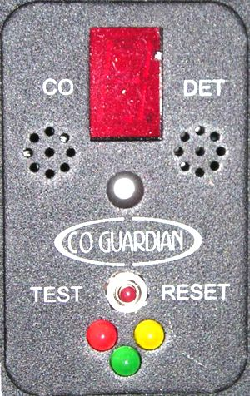
\includegraphics{../Diagrams/co}}


The CO Guardian Aero 252F CO Monitor provides visual and aural indications of CO levels that exceed 40 PPM. The CO Monitor is located on the lower left side of the cockpit, ahead of the fuel selector. It is powered from the Main Bus, and has an ON/OFF toggle switch to its right.

The unit is designed to operate in temperatures of -1\textdegree C to 49\textdegree C.

\textbf{Self-Test} --- The unit performs a self-test upon power application, or when the TEST/RESET button on its face is pressed. A successful self-test provides the following indications in sequence:
\begin{itemize}
\item Display shows 0 
\item Aural alert sounds two beeps 
\item Green, Yellow and Red LEDs flash in sequence 
\item Display counts up from 1 to 9 then 0 
\item Aural alert sounds one beep 
\item Yellow LED flashes 
\item Display goes blank 
\item Green LED remains illuminated, with the Yellow and Red LED OFF 
\end{itemize}
\textbf{Digital Display} --- The digital display remains blank for CO concentrations of less than 40 PPM. It flashes two digits in sequence for CO concentrations of between 40 and 99 PPM (e.g. alternating 5 and 0 indicates 50 PPM). CO concentrations of greater than 100 PPM will be displayed as a single, steady digit equal to the hundreds unit (e.g. steady 5 means 500 PPM). The digital display shows the CO level without delay.

\textbf{Aural Indications} --- The unit has a built-in speaker. It is not connected to the intercom. CO concentrations of greater than 50 for a specified time delay are annunciated by beeps and flashes of the Yellow LED or Red LED.


\textbf{Normal Indications} --- If the CO concentration is less than 40 PPM, the Green light will be illuminated, the display will be blank and there will be no aural alerts. If the CO concentration is between 40 and 50 PPM, the display will alternate between 4 and 0, and the Green light will remain illuminated.

\begin{minipage}{\textwidth}
\textbf{CO Alarm Indications} --- CO values of 50 PPM or greater are indicated as follows:
\begin{center}
\begin{tabular}
{|c|c|c|} \hline CO Conc. (PPM) & Aural Alarm Delay& LED that will be lit\tabularnewline \hline \hline Less than 50 & No alarm& Green\tabularnewline \hline 50-70& 10 minutes & Yellow\tabularnewline \hline 70-150 & 5 minutes& Red\tabularnewline \hline 200& 3 minutes & Red\tabularnewline \hline 300& 1 minute& Red\tabularnewline \hline 400& No delay & Red\tabularnewline \hline 
\end{tabular}
\end{center}
\end{minipage}

\textbf{System Failures} --- System failures are indicated as follows:
\begin{itemize}
\item Flashing Green, Red and Yellow LEDs + beep every 30s CO --- sensor failure 
\item Flashing Red LED + beep every 30s --- temperature sensor failure 
\item Flashing Yellow LED + beep every 30s --- humidity sensor failure 
\item Any other combination of flashing LEDs + beep every 30s --- micro-controller failure 
\end{itemize}

\section{FIRE EXTINGUISHER}

A 2.5 lb halon fire extinguisher is mounted in a bracket on the floor on the left side  of the cockpit below the rear seat throttle. The cockpit must be ventilated after using the fire extinguisher.

\section{EMERGENCY LOCATOR TRANSMITTER} 
\piccaption{ELT Remote Control} 
\parpic[r]{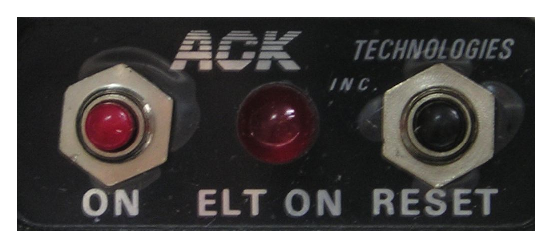
\includegraphics{../Diagrams/elt1}}

The aircraft is fitted with an ACK E-04 406 MHz Emergency Locater Transmitter (ELT). The ELT is mounted in in the aft baggage area, on a tray at the forward right side. The ELT remote control is located on the upper right side of the instrument panel. The ELT may be selected ON by a momentary press of the ON button on the left side of the remote control. The red ON light will flash when the ELT is transmitting. The ELT may be selected OFF by a momentary press of the RESET button. An aural alert will sound every 50 s when the ELT is transmitting.

The ELT has a three-position switch. This switch should be in the ARMED position for flight, in which case it is covered with a red plastic cap which retains it in the ARMED position. The ON position is used to force the ELT to transmit after removing it from the aircraft and connecting the telescopic antenna. 
\begin{figure}
[htb]

% 
\centering 
\begin{minipage}{3in}

%
\centering 
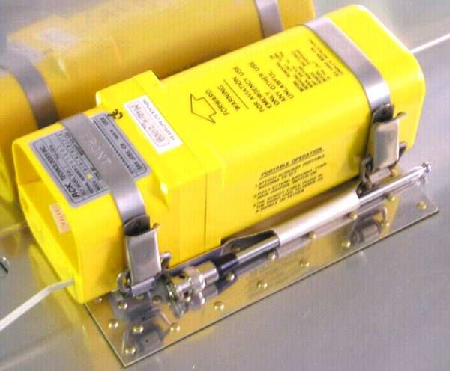
\includegraphics[scale=0.8]{../Diagrams/elt2} \caption{ELT in Tray} 
\end{minipage}

% 
\qquad 
\begin{minipage}{3in}

%
\centering 
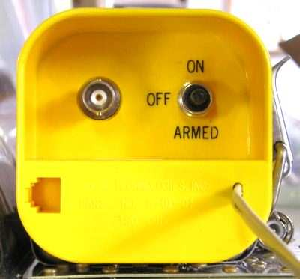
\includegraphics[scale=1]{../Diagrams/elt3} \caption{ELT Main Control}

% 
\end{minipage}

% 
\end{figure}

Following an emergency landing, the ELT may be removed from the aircraft if required. It is secured to the tray by two over-centre locks on band-clamps. The phone line going to the remote transmitter and the antenna coax cable must both be removed. The loose end of the phone line may be clipped into the receptacle on the ELT to make a loop that can be used as a handle. There is a telescopic antenna clipped to the mounting tray which must be connected to the coax mount on the ELT to allow it to transmit once it is removed from the aircraft. 

\section{FIRST AID KIT}
A first aid kit in a red zippered pouch is attached to the left side of the rear cockpit side wall.

\cleardoublepage 

% !iTeXMac(input): POH.tex
\chapter{AIRPLANE HANDLING, SERVICE \& MAINTENANCE} \vspace{\minitocspacebefore} \minitoc \cleardoublepage

\section{INTRODUCTION} This is a place-holder for the Airplane Handling, Service \& Maintenance Section. The section will be completed once in-service experience has been gained.

\section{GROUND HANDLING}
Ground motion is best accomplished by pushing or pulling on the propeller as near to the
spinner as possible. The following are recommended additional pushing locations to help move the
airplane: 

\begin{itemize*}
  \item Moving forward --- front seat support (canopy open).
  \item Moving rearwards --- wing leading edges and roots of horizontal stabilizer.
  \end{itemize*}

A suitable pushbar may be fitted over the two ends of the tailwheel axle.

Take care to not use high power during run-up, as the tail will lift even if the control stick is held full aft.

Wing tie down mounting points are located centrally under each wing. Use a 3/8" dia x 16
tpi eye bolt to attach tie down rope to airplane. Secure a third line to the tail wheel spring.

\subsection{Canopy Protection and Ventilation}
If the aircraft is tied down outdoors and subject to weather elements for any length of time, then the use of an aircraft canopy cover is highly recommended. The cover will protect canopies and windows from abrasive dust, dirt, and sand kicked up by wind or prop wash. Before purchasing, verify that the canopy cover is NOT waterproof as the trapped moisture and heat from the sun can be deleterious. Acrylic subjected to this treatment over a period of time may turn slightly milky and eventually crazes.

Keep the canopy ventilated or covered when the aircraft is parked in the hot sun. Cabin temperatures can easily reach 150-200 degrees F even on a mild day. The acrylic can generally take these temperature conditions multiple times without any apparent adverse effect, but the cumulative affect that will cause shortened service life. The use of a canopy cover will significantly reduce the internal temperatures inside the aircraft to just a few degrees above outside ambient temperatures. Additionally it will also protect the avionics from heat and the upholstery/seat belt harnesses from harmful UV rays.

\section{SERVICING}
\subsection{Brakes}
The brake fluid reservoir is located on the engine side of the firewall near the upper left side.  The preferred brake fluid is MIL-PRF-83282, but MIL-H-5606 fluid can mixed if required.  Note that MIL-H-5606 has a much lower flash point, so should be avoided if possible.

The original O-rings in the brake calipers were replaced with Viton O-rings, due to the much higher acceptable temperature of Viton.

\section{CLEANING AND CARE}
\subsection{Windscreen and Canopy}
The windscreen and canopy are fabricated from polymethyl methacrylate) (PMMA), an acrylic plastic, brand name Plexiglas.

\subsubsection{Cleaning}
For general cleaning use Dawn dishwashing liquid or equivalent and water followed by a clear water rinse. To prevent water spots, blow dry with compressed air or wipe dry with soft cotton flannel. Plexus, Sprayaway \#848 Industrial Plastic Cleaner, or All Clear can also be used for day to day cleaning. Grease, oil, tape residue, etc. may best be removed with Mineral spirits, refined kerosene, white gasoline, naphtha, or isopropyl alcohol. Wash approved solvents off of canopy with Dawn dishwashing liquid and water. It is best to avoid using products that are not specifically formulated for acrylics (such as Rain-X or Lemon Pledge) on the canopy.

\begin{Note}[CAUTION]DO NOT use Loctite, aromatic solvents, acetone, benzene, ethyl acetate, carbon tetrachloride, lighter fluid, lacquer thinners, gasoline, toluene, window sprays, concentrated alcohols, keytones, scouring compounds, ammonia, or 409 cleaner on or around acrylic canopy materials.
\end{Note}

\subsubsection{Scratch Removal}
Small scratches can be buffed out with Meguiar's Mirror Glaze \#17. For deep scratch removal, use Scratch Off , Micro Mesh, or 3M Window Repair kits. Avoid removing scratches in critical areas where clear visibility is important, as the process will usually result in some degree of optical distortion.

\section{COWLING REMOVAL} \textcolor{red}{See C-GFEW POH for example.}

\section{INSPECTION PANELS}
In addition to the engine cowling, the aircraft has a number of inspection and access panels:
\begin{enumerate*}
  \item Oil dipstick access door on aft right side of upper cowling.
  \item Instrument panel access door on aft wall of forward baggage compartment. Four Torx T10 screws are removed, allowing the access panel to be opened.
  \item Three under-wing inspection panels on each wing provide access to fuel tank securing bolts and aileron bellcranks.
  \item Rear fuselage inspection plates on each side provide access to the elevator horns.
  \item Rear baggage compartment aft wall and hat shelf are removable, providing access to the battery and rear fuselage.
  \item Cockpit and rear baggage compartment floors are removable.
  \item Wing tips are removable, but note that they must remain close to the wing tips due to the coax connections to an internal antenna in each wing tip, and the power wires for the strobe and navigation lights in each wing tip.
  \end{enumerate*}

\begin{Note}[CAUTION]
The ADS-B must not be powered up unless an ADS-B antenna is connected to it.  If the middle right wing inspection panel is removed, and it is desired to power up the aircraft, either:
\begin{enumerate*}
	\item Remove the fuse for the ADS-B transmitter, or
	\item Uplug the wiring harness from Echo UAT ADS-B transmitter, on the bottom of the avionics shelf below the instrument panel, or
	\item Connect the ADS-B antenna to its coax.
\end{enumerate*}
\end{Note}

\needspace{10\baselineskip}
\section{INITIAL INSPECTIONS}

The following inspections are required following first flight:

\subsection{After First Flight} 
\begin{enumerate*}
	\item Complete firewall forward detailed visual inspection. 
	\item Check alternator belt tension (7 -- 9 ft-lb on pulley when belt slips). 
	\item Complete airframe visual detailed inspection. 
\end{enumerate*}

%\subsection{2 Hours} 
%\begin{enumerate*}
%	\item Lubricate propeller hub. See 100 Hour Inspection or Hartzell Propeller Owner's Manual for details of procedure. 
%\end{enumerate*}

\subsection{10 Hours} 
\begin{enumerate*}
	\item Change oil, cut open oil filter and inspect, and inspect suction screen. Look for metal particles, shavings or flakes. Info from Lycoming Service Bulletin No. 480D, July 13, 2000. 
	\item Retorque landing gear bolts.
	\item Complete items from Conditional Inspection, except for oil change, propeller lubrication, ELT. 
\end{enumerate*}

\subsection{25 Hours} 
\begin{enumerate*}
	\item Check alternator belt tension (7 -- 9 ft-lb on pulley when belt slips). 
\end{enumerate*}

\subsection{35 Hours} 
\begin{enumerate*}
	\item Change oil, cut open oil filter and inspect, and inspect suction screen. Look for metal particles, shavings or flakes. Info from Lycoming Service Bulletin No. 480D, July 13, 2000. 
	\item Complete items from Conditional Inspection, except for oil change, propeller lubrication, ELT. 
\end{enumerate*}

\section{PERIODIC MAINTENANCE} This section includes all items specified in the Lycoming Owner's Manual, MT Operation and Installation manual and Christen 801 Series Inverted Oil System Product Manual. \textcolor{red}{Add items from Slick mag service info.} It is supplemented by recommendations from Van's Aircraft, other RV owners, and engineering judgement.

\subsection{50 Hours or 4 months} The following items should be performed every 50 hours, or four months, whichever comes first:
\begin{enumerate*}
	\item Drain oil sump with oil hot. Send sample for analysis (see Lycoming Service Letter No. 171). 
	\item Replace oil filter. Cut open \& inspect. 
	\item Inspect \& clean suction oil screen. 
	\item Check \& record brake fluid level. 
	\item Check integrity of: 
	\begin{enumerate*}
		\item Fuel \& oil hoses, 
		\item Ignition system, 
		\ifthenelse{\thePMAG = 0}{\item Magneto P-lead \& mounting bolts, }{\item PMag wiring at connector \& mounting bolts}
		\item Exhaust system \& attachment hardware, 
		\item Cylinders - check for oil leak at rocker box covers, and check for signs of overheating (burned paint), 
		\item Baffling/plenum, 
		\item Firewall forward wiring, 
		\item Engine mount bolts, 
		\item Firewall seals, and 
		\item Cowling hinge eyes. 
	\end{enumerate*}
	\item Inspect \& lubricate: 
	\begin{enumerate*}
		\item Throttle, mixture \& prop linkages, 
		\item Alternate air door \& control, and 
		\item Oil cooler door \& control. 
		\item Tail wheel (disassemble, inspect locking pin for burrs, lubricate and reassemble) 
	\end{enumerate*}
	\item Check alternator belt condition \& tension. 
	\item Check tires for wear, rotate/replace as necessary. 
	\item On test flight, log engine data. 
\end{enumerate*}

\subsection{100 Hours or 12 months} The following items should be performed every 100 hours, or 12 months, whichever comes first: 
\begin{enumerate*}
	\item Complete the items from the 50 hour inspection, plus 
	\item Remove, clean, inspect and regap spark plugs.
	\item Inspect \& clean gascolator screen. 
	\item Inspect \& clean fuel filter. \textcolor{red}{Check recommended interval.} 
	\item Conduct compression check on all cylinders. 
	\item Propeller 
	\begin{enumerate*}
		\item Remove spinner 
		\item Inspect spinner and back plate. 
		\item Check propeller mounting bolts and safety wire. 
		\item Inspect prop blades for nicks and cracks. 
		\item Inspect prop hub for cracks or grease leakage. \textcolor{red}{Add any items from MT manuals}. 
		\item Check blade track. 
		\begin{enumerate*}
			\item Chock the wheels securely. 
			\item Place a fixed reference point beneath the propeller, within 0.25" below the lowest point of the propeller arc. Fasten a sheet of paper to the reference point. 
			\item Rotate the propeller by hand (opposite the direction of normal rotation) until a blade points directly at the paper. Mark the position of the blade tip on the paper. 
			\item Repeat the procedure with the second blade. 
			\item Tracking tolerance is 0.125" between the position of the two blades. 
		\end{enumerate*}
		\item Reinstall the spinner. 
	\end{enumerate*}
	\item Check alternator belt tension (7 -- 9 ft-lb on pulley when belt slips). 
\ifthenelse{\thePMAG = 1}{
	\item PMag Electronic Ignition
	\begin{enumerate*}
		\item Check E-Mag website for Service Bulletin compliance.
		\item Check PMag thermal sticker for exceedence. 
		\item Check PMag ignition lead resistance is approximately $180\Omega$ per foot.  Confirm the resistance is approximately stable while bending, twisting and tugging each end.
		\item Check PMag plug gaps.
		\item Remove PMag and check for smooth rotation and no excessive lateral or axial play in shaft. 
		\item Torque wire lead connection screws to 5 in--lb.
		\item Set PMag timing. 
	\end{enumerate*}}
{	\item Magneto
	\begin{enumerate*}
		\item Check breaker points for pitting and minimum gap, 
		\item Check for excessive oil in breaker compartment, 
		\item Lubricate breaker point felt, and 
		\item Check Magneto to Engine timing. See Lycoming Direct Drive Overhaul Manual for details of procedure.
	\end{enumerate*}}
	\item Light Speed Electronic Ignition
	  \begin{enumerate*}
	    \item Remove Hall Effect Sensor and open up to check for gear, bearing and seal wear
	    \item Set electronic ignition timing
    	\end{enumerate*} 	
	\item Check cylinders visually for cracked or broken fins, 
	\item Check engine mounting bolts and bushings, 
	\item Check fuel injector nozzles for looseness, tighten to 60 in-lb torque, 
	\item Check fuel lines for dye stains at connections, and 
	\item Re-install spark plugs with new washers. 
\end{enumerate*}

\subsection{400 Hours} The following items should be performed every 400 hours: 
\begin{enumerate*}
	\item Replace spark plugs, and 
	\item Remove rocker box covers and check for freedom of valve rockers when valves are closed. Look for evidence of abnormal wear or broken parts in the area of valve tips, valve keeper, springs and spring seats. 
\end{enumerate*}

\subsection{500 Hours} The following items should be performed every 500 hours or 36 months:
\begin{enumerate*}
\ifthenelse{\thePMAG = 0}{\item\textcolor{red}{Insert Slick's recommended items.}}{}
	\item Light Speed Electronic Ignition: 
	\begin{enumerate*}
		\item Replace high tension leads (i.e. coil to spark plug wires), and 
	\end{enumerate*}
\end{enumerate*}

\subsection{1500 Hours} The following items should be performed every 1500 hours or 10 years (from CAR 625 Appendix C --- not mandatory for amateur-built aircraft). MT's recommended overhaul interval is 1800 hrs or 72 months.
\begin{enumerate*}
	\item Overhaul propeller. 
\end{enumerate*}

\subsection{3 Months} The ELT Self Test must be performed every 3 months:
\begin{enumerate*}
	\item Battery Master Switch is OFF.
	\item ELT Switch is ARMED.
	\item Press Test/Reset Button on ELT Remote Control (right most button).
	\item ELT Remote Control Lamp should flash once.
	\item A single beep will sound if the ELT passes the self test.
	\item Two to Five beeps will sound if there is a problem:
	\begin{enumerate*}
	  \item 2 beeps, followed by 2 second delay, followed by 2 beeps: battery low.
	  \item 3 beeps, followed by 2 second delay, followed by 3 beeps: low RF power.
	  \end{enumerate*}
	\item Check for email from Canadian Beacon Registry confirming reception of the ELT signal by the satellite network.
\end{enumerate*}

\subsection{12 Months} The following items must be performed every 12 months (the due date is exactly 12 months following the previous inspection):
\begin{enumerate*}
	\item Conduct compass swing of any non-stabilized magnetic compass and install dated compass card (requirement from CAR 625 App. C).
	\item Inspect ELT (requirement from CAR 625 App. C).
\end{enumerate*}

\subsection{24 Months} The following items must be performed every 24 months (the due date is exactly 24 months following the previous inspection):
\begin{enumerate*}
	\item Calibrate altimeter and altitude encoder IAW AWM 571 App. B (requirement from CAR 625 App. C).
	\item Test transponder IAW AWM 571 App. F (requirement from CAR 625 App. C).
\end{enumerate*}

\section{ANNUAL INSPECTION} An annual inspection must be carried out once every 12 months (the due date is the end of the 12th month following the previous inspection). The inspection must include all items listed in CAR 625 Appendix B. The following list expands on the required items. Items marked with (*) are not required as per CAR 625 Appendix B. Completion of these items is not required as per the CARs, but is strongly recommended to improve reliability and safety.

\begin{enumerate*}
	\item{AD Review}
	\begin{enumerate*}
		\item Print list of applicable ADs from TC web site.\dotfill $\bigbox$
		\item Comply with ADs during inspection as required.\dotfill $\bigbox$
	\end{enumerate*}

  \item{Aircraft General}
  \begin{enumerate*}
    \item Remove or open all inspection panels, access doors, fairings and cowlings. \dotfill $\bigbox$
    \item Thoroughly clean the aircraft. \dotfill $\bigbox$
    \item Inspect panel, door and cowling closing and locking mechanisms for improper installation, function and condition. \dotfill $\bigbox$
		\end{enumerate*}

	\item{Engine} 
\ifthenelse{\thePMAG = 1}{\begin{Note}[WARNING] \centering Ground PMag before working on engine. \end{Note}}
{\begin{Note}[WARNING] \centering Ground mags before working on engine. \end{Note}}
	\begin{enumerate*}
		\item Remove engine cowl.\dotfill $\bigbox$
		\item Cowling --- clean it and inspect for cracks, distortion and loose or missing fasteners.\dotfill $\bigbox$
		\item Leaks --- inspect engine, oil lines, oil cooler and inverted oil system for oil leaks.\dotfill $\bigbox$
		\item Oil 
		\begin{enumerate*}
			\item Oil temp. sender --- inspect for leaks and security. \dotfill $\bigbox$
			\item Oil lines and fittings --- inspect for leaks, chafing security, dents and cracks. \dotfill $\bigbox$
			\item Oil cooler --- clean cooling fins and inspect condition. (*)\dotfill $\bigbox$
			\item Inverted oil system --- inspect for for leaks and security. \dotfill $\bigbox$
			\item Screens and sump drain plugs --- inspect for metal particles and foreign matter. \dotfill $\bigbox$
			\item Fill engine with oil per \textcolor{red}{lubrication chart}. \dotfill $\bigbox$
		\end{enumerate*}
		\item Ignition (*)
		\begin{enumerate*}
			\item Check condition of spark plugs and adjust gap. \dotfill $\bigbox$
			\item Check ignition harness and insulators. \dotfill $\bigbox$
\ifthenelse{\thePMAG = 0}{\item Check magneto points for proper clearance maintain at \textcolor{red}{.018 $\pm $ .006}. \dotfill $\bigbox$
			\item Check magneto for oil seal leaks. \dotfill $\bigbox$
			\item Check breaker felt for proper lubrication. \dotfill $\bigbox$
			\item Check distributor block for cracks, burned areas or corrosion. \dotfill $\bigbox$
			\item Check magnetos to engine timing. See Lycoming Direct Drive Overhaul Manual for details of procedure. \dotfill $\bigbox$}
			{\item Check E-Mag website for Service Bulletin compliance. \dotfill $\bigbox$
			\item Check PMag thermal sticker for exceedence. \dotfill $\bigbox$
			\item Check PMag ignition lead resistance is approximately $180\Omega$ per foot.  Confirm the resistance is approximately stable while bending, twisting and tugging each end.  \dotfill $\bigbox$
			\item Remove PMag and check for smooth rotation and no excessive lateral or axial play in shaft. \dotfill $\bigbox$
			\item Torque PMag wire lead connection screws to 5 in--lb. \dotfill $\bigbox$
			\item Set PMag timing. \dotfill $\bigbox$}
			\item Remove Light Speed electronic ignition Hall Effect Sensor and open up to check for gear, bearing and seal wear. \dotfill $\bigbox$
			\item Set Light Speed electronic ignition timing. \dotfill $\bigbox$
		\end{enumerate*}
		\item Thoroughly clean engine and other items ahead of the firewall. \dotfill $\bigbox$
		\item Studs and nuts --- inspect for defects, evidence of improper torque and safety locking. \dotfill $\bigbox$
  	\item Cylinder compression --- conduct compression check on all cylinders. Record readings: \\* \hfill \#1:\underline{\makebox[0.5in][l]{}} \\* \hfill \#2:\underline{\makebox[0.5in][l]{}} \\* \hfill \#3:\underline{\makebox[0.5in][l]{}} \\* \hfill \#4:\underline{\makebox[0.5in][l]{}} \\* If compression test indicates problems, check internal condition and tolerances. \dotfill $\bigbox$
		\item Remove air filter and clean. \dotfill $\bigbox$
		\item Check condition of alternate air door and cable. \dotfill $\bigbox$
		\item Fuel Injection System
		\begin{enumerate*}
  		\item Inspect fuel injection servo. \dotfill $\bigbox$
  		\item Inspect condition of fuel injection lines IAW FAA AD 2011-26-04 \& Lycoming MSB 342G. \dotfill $\bigbox$
		\end{enumerate*}
		\item Clean screens in fuel pump. \dotfill $\bigbox$
		\item General condition: \dotfill $\bigbox$
		\begin{enumerate*}
		\item Check engine controls throttle, carb heat, mixture, prop and alternate air door. Check condition, proper travel and safety locking. \dotfill $\bigbox$
		\item Exhaust system --- inspect for cracks, defects and improper attachment. \dotfill $\bigbox$
		\item Inspect heater muffs, heater boxes and SCAT tubes. \dotfill $\bigbox$
		\item Check breather tube for obstructions and security. \dotfill $\bigbox$
		\item Check crankcase for cracks, leaks, security of bolts. \dotfill $\bigbox$
		\item Engine mounts --- inspect for cracks, looseness of mounting and looseness of engine to mount. \dotfill $\bigbox$
		\item Flexible vibration dampeners --- inspect for poor condition and deterioration. \dotfill $\bigbox$
		\item Check all engine baffles and plenum parts. \dotfill $\bigbox$
		\item Check firewall seals. \dotfill $\bigbox$
		\item Check condition and tension of alternator, alternator mount, drive belt and B-lead. \dotfill $\bigbox$
		\item Check condition of starter, starter mount, starter cable and solenoid. \dotfill $\bigbox$
		\item Inspect all starter power and ground connections ahead of firewall and clean as necessary. \dotfill $\bigbox$
		\item Check standby alternator. \dotfill $\bigbox$
		\item Check prop governor. \dotfill $\bigbox$
		\item Internal corrosion --- inspect engines which have not been inhibited and have been out of \\service in excess of 12 months. \dotfill $\bigbox$
	  \end{enumerate*}
		\item Check \& record brake fluid level. (*) \dotfill $\bigbox$
		\item Lubricate all controls. \dotfill $\bigbox$
		\item Reinstall engine cowl. \dotfill $\bigbox$
	\end{enumerate*}
	\item{Fuel System} 
	\begin{enumerate*}
		\item Clean and inspect fuel filter. \dotfill $\bigbox$
		\item Clean and inspect gascolator. \dotfill $\bigbox$
		\item Inspect condition of fuel lines. \dotfill $\bigbox$
		\item Check fuel system for leaks. \dotfill $\bigbox$
		\item Check pressure from electric fuel pump is 25 -- 45 psi. Record pressure: \underline{\makebox[0.5in][l]{}} \dotfill $\bigbox$
		\item Check operation of fuel selector valve. \dotfill $\bigbox$
		\item Check fuel vents. \dotfill $\bigbox$
	\end{enumerate*}

	\item{Propeller} 
	\begin{enumerate*}
	  \item Propeller hub assembly --- inspect for cracks, nicks, binding and oil leakage. \dotfill $\bigbox$
	  \item Bolts and nuts --- inspect for improper torque and safety locking. \dotfill $\bigbox$
	  \item Control mechanisms --- inspect for improper operation, insecure mounting and improper range of \\travel. \dotfill $\bigbox$
	  \item Composite blades --- inspect for:
	  \begin{enumerate*}
	    \item cracks, bruises, scars, warping, evidence of glue failure and delamination, \dotfill $\bigbox$
	    \item attachment bolt tightness, and \dotfill $\bigbox$
	    \item correct track, excessive rotational and end play. \dotfill $\bigbox$

  	  \end{enumerate*}
  	\item Spinner assembly --- inspect for cracks and wear. \dotfill $\bigbox$
  	\item Variable pitch propellers --- check correct operation during ground run. \dotfill $\bigbox$
	\end{enumerate*}


	\item{Cockpit} 
	\begin{enumerate*}
		\item Remove seats and cockpit floors. \dotfill $\bigbox$
		\item Generally --- inspect for dirt and loose equipment that might foul the controls. \dotfill $\bigbox$
		\item Inspect cockpit area, forward fuselage and underfloor area for corrosion, cracks, chafed wiring, deterioration, distortion, evidence of failure, defective or insecure attachment fittings, etc. \dotfill $\bigbox$
		\item Check for dirt and loose equipment that might foul the controls. \dotfill $\bigbox$
		\item Check all wing front spar attachment bolts. \dotfill $\bigbox$
		\item Check rear spar carry through structure. \dotfill $\bigbox$
		\item Inspect COM 1 and transponder antennae and coax. \dotfill $\bigbox$
		\item Landing gear boxes --- inspect condition of wiring, etc. Check for FOD. \dotfill $\bigbox$
		\item Landing gear attach bolts --- Check torque \dotfill $\bigbox$
		\item Controls:
  	\begin{enumerate*}
  		\item Check control columns, systems and connection. \dotfill $\bigbox$
  		\item Lubricate control column bearings as required. \dotfill $\bigbox$
  		\item Check pitch and roll trim operation from front and rear seats. \dotfill $\bigbox$
  		\item Check flap motor, wiring and pushrods. \dotfill $\bigbox$
  		\item Lubricate flap pushrod bearings as required. \dotfill $\bigbox$
  	  \end{enumerate*}
		\item Reinstall cockpit floors and front seat. \dotfill $\bigbox$
		\item Windscreen and canopy --- inspect for deterioration and breakage. \dotfill $\bigbox$
		\item Windscreen and canopy --- inspect canopy tracks, rollers and latch. \dotfill $\bigbox$
		\item Canopy Latch --- disassemble, inspect, lubricate and reassemble. \dotfill $\bigbox$
		\item Upholstery --- inspect for security and tears. (*) \dotfill $\bigbox$
		\item Seats and safety belts --- inspect for poor condition, fraying, and any other apparent defects. \dotfill $\bigbox$
		\item Rudder pedals, brake cylinders, parking brake valve and brake lines --- check condition. \dotfill $\bigbox$
		\item Gooseneck and instrument lights --- check condition and function of lamps and dimmers. \dotfill $\bigbox$
		\item Instrument Panel:
  	\begin{enumerate*}
  		\item Instruments --- inspect for poor condition, mounting, marking and, where practicable, for \\improper operation. \dotfill $\bigbox$
  		\item Placards ---- confirm all placards listed in the POH are in place and are legible. \dotfill $\bigbox$
  		\item Static System --- conduct static system leak check. (*) \dotfill $\bigbox$
      \end{enumerate*}
		\item Check condition of heater controls. \dotfill $\bigbox$
		\item Check condition of throttle, mixture and propeller speed controls. \dotfill $\bigbox$
		\item Check condition of oil cooler door and alternate air controls. \dotfill $\bigbox$
		\item Check condition and operation of air vents. \dotfill $\bigbox$
		\item Check fire extinguisher. \dotfill $\bigbox$
		\item Check wire bundles for chafing, paying particular attention to Infinity stick grip wire bundle at \\bottom of stick. \dotfill $\bigbox$
	\end{enumerate*}
	\item{Aft Fuselage} 
	\begin{enumerate*}
		\item Remove aft baggage floor and aft baggage rear bulkhead. \dotfill $\bigbox$
		\item Check under whole aft fuselage, including skins, bulkheads, longerons, stiffeners ,under baggage floor area for corrosion, cracks, chafed wiring, deterioration, distortion, evidence of failure, defective or insecure attachment fittings, etc. \dotfill $\bigbox$
		\item Battery --- inspect for improper installation and improper charge. Inspect battery hold-down and \\battery cables. Check battery voltage with no load. \dotfill $\bigbox$
		\item Strobe power supply --- Check condition and wiring. \dotfill $\bigbox$
		\item GPS antenna --- check condition of antenna and coax cable. \dotfill $\bigbox$
		\item Elevator bellcrank and elevator control tubes --- check condition. Lubricate bellcrank and \\pushrod ends as required. \dotfill $\bigbox$
		\item Reinstall aft baggage floor and aft baggage rear bulkhead. \dotfill $\bigbox$
	\end{enumerate*}
  \item{ELT} 
  \begin{enumerate*}
  	\item Inspect mounting tray and fasteners. \dotfill $\bigbox$
  	\item Inspect coax cable for abrasion. Disconnect coax connections and inspect jack and plug for corrosion. \dotfill $\bigbox$
  	\item Inspect cable to remote control for abrasion. Disconnect connections and inspect for corrosion. \dotfill $\bigbox$
  	\item Inspect GPS data cable for abrasion. Disconnect GPS data cable and inspect jack and plug for \\corrosion. \dotfill $\bigbox$
  	\item Check expiration date of ELT, aural alert and remote batteries and replace if they will expire \\within the next 12 months. \dotfill $\bigbox$
  	\item Conduct g-switch test from FAA Order 8250.3. From ACK manual, page 13. (*) \dotfill $\bigbox$
  	\begin{enumerate*}
  		\item Remove ELT from tray. \dotfill $\bigbox$
  		\item Select ELT switch to ARMED. \dotfill $\bigbox$
  		\item Monitor 121.5, with squelch turned OFF. \dotfill $\bigbox$
  		\item During first five minutes of the hour, test g-switch: 
  		\begin{enumerate*}
  		  \item hold the ELT at your waist with the arrow printed on the battery case facing away from you. \dotfill $\bigbox$
  		  \item move the ELT rapidly away from your waist. \dotfill $\bigbox$
  		  \item when the ELT reaches the full extent of your arm retract it back to your waist as fast \\as possible. \dotfill $\bigbox$
  		  \end{enumerate*} 
  		\item Verify that the ELT tone is heard. \dotfill $\bigbox$
  		\item Select ELT switch to OFF within 30 s (406 MHz emergency signal is sent 50 s after g-switch activation). \dotfill $\bigbox$
  	\end{enumerate*}
  	\item Reinstall ELT \dotfill $\bigbox$
  	\item Set ELT switch to ARMED \dotfill $\bigbox$
  	\item Replace red guard over ELT switch \dotfill $\bigbox$
  	\item Reseal DIN connector with tape \dotfill $\bigbox$
  	\item Perform ELT Self Test, due every three months \dotfill $\bigbox$
  \end{enumerate*}
	\item{Empennage} 
	\begin{enumerate*}
		\item Remove empennage fairing and elevator horn inspection covers. \dotfill $\bigbox$
		\item Check horizontal stabilizer attachment. \dotfill $\bigbox$
		\item Check vertical fin attachments. \dotfill $\bigbox$
		\item Check vertical fin and rudder surfaces. \dotfill $\bigbox$
		\item Check rudder horn and attachment. \dotfill $\bigbox$
		\item Check rudder bolts for wear. \dotfill $\bigbox$
		\item Check rudder strobe and nav light for security. \dotfill $\bigbox$
		\item Check horizontal stabilizer and elevators. \dotfill $\bigbox$
		\item Inspect horizontal stabilizer front spar IAW SB 14-01-31. \dotfill $\bigbox$
		\item Record SB 14-01-31 inspection in logbook. \dotfill $\bigbox$
		\item Check elevator trim tab and servo. \dotfill $\bigbox$
		\item Check elevator horn. \dotfill $\bigbox$
		\item Check elevator bolts for wear. \dotfill $\bigbox$
		\item Inspect elevator spar IAW SB 14-02-05. \dotfill $\bigbox$
		\item Record SB 14-02-05 inspection in logbook. \dotfill $\bigbox$
		\item Lubricate all bearings as needed. \dotfill $\bigbox$
		\item Reinstall empennage fairing and elevator horn inspection covers. \dotfill $\bigbox$
	\end{enumerate*}
	\item{Wings} 
	\begin{enumerate*}
		\item Remove wing root fairing and under-wing inspection panels. \dotfill $\bigbox$
		\item Check fuel tank to fuselage mount. \dotfill $\bigbox$
		\item Check wing rear spar attachment bolts. \dotfill $\bigbox$
		\item Check surfaces for damage and loose rivets. \dotfill $\bigbox$
		\item Check wing walk condition. \dotfill $\bigbox$
		\item Check flaps and pushrods. \dotfill $\bigbox$
		\item Check fuel tank bolts on front spar. \dotfill $\bigbox$
		\item Check aileron bellcrank and control tubes. \dotfill $\bigbox$
		\item Inspect rear wing spar for cracks IAW SB 16-03-28. \dotfill $\bigbox$
		\item Record SB 16-03-28 inspection in logbook. \dotfill $\bigbox$
		\item Lubricate aileron bellcrank and pushrods as required. \dotfill $\bigbox$
		\item Check aileron mounts and attachments. \dotfill $\bigbox$
		\item Lubricate aileron hinges as required. \dotfill $\bigbox$
		\item Check landing and taxi lights and lenses - condition and function. \dotfill $\bigbox$
		\item Check nav lights and strobes - condition and function. \dotfill $\bigbox$
		\item Check wing tips. \dotfill $\bigbox$
		\item Remove wing tips and inspect internal antennae. \dotfill $\bigbox$
		\item Reinstall wing root fairing and under-wing inspection panels. \dotfill $\bigbox$
	\end{enumerate*}
	\item{Wheels and Brakes} 
	\begin{enumerate*}
		\item Tail wheel assembly. 
		\begin{enumerate*}
		  \item Tail wheel pivot --- disassemble. \dotfill $\bigbox$
		  \item Tail wheel pivot and locking mechanism --- inspect and lubricate. \dotfill $\bigbox$
		  \item Tail wheel axle --- disassemble. \dotfill $\bigbox$
		  \item Tail wheel bearings --- inspect and lubricate. \dotfill $\bigbox$
		  \item Tail wheel axle and tail wheel assembly --- reassemble and reinstall on aircraft. \dotfill $\bigbox$
	  \end{enumerate*}
		\item Wheel pants and gear leg fairings --- remove. \dotfill $\bigbox$
		\item Wheels --- remove. \dotfill $\bigbox$
		\item Wheels --- inspect for cracks, corrosion, defects broken bolts and condition of bearings. \dotfill $\bigbox$
		\item Wheel bearings --- clean, inspect and repack. \dotfill $\bigbox$
		\item Tires - inspect for wear, cuts and incorrect inflation; inspect for improper installation and improper operation. Rotate as required. \dotfill $\bigbox$
		\item Brake lining --- inspect. Minimum acceptable lining thickness is 0.100\" \dotfill $\bigbox$
		\item Brake disc --- inspect. Minimum acceptable disc thickness is 0.167\" \dotfill $\bigbox$
		\item Landing gear legs --- inspect. \dotfill $\bigbox$
		\item Wheels --- reinstall. \dotfill $\bigbox$
		\item Brake lines --- inspect for leaks and condition. \dotfill $\bigbox$
		\item Landing gear wear plate at lower fuselage longeron --- inspect. \dotfill $\bigbox$
		\item Wheel pants, gear leg fairings and intersection fairings --- inspect. \dotfill $\bigbox$
		\item Tire Pressure --- check. Record tire pressures. L:\underline{\makebox[0.5in][l]{}}, R:\underline{\makebox[0.5in][l]{}} \dotfill $\bigbox$
		\item Wheel pants and gear leg fairings --- reinstall. \dotfill $\bigbox$
	\end{enumerate*}
	\item{Operational Inspection} 
	\begin{enumerate*}
		\item Check items that wouldn't normally be checked in flight. \textcolor{red}{Which items??} \dotfill $\bigbox$
		\item Pitot Heat --- check. \dotfill $\bigbox$
	\end{enumerate*}
	\item{Engine Ground Run}
	\begin{enumerate*}
		\item Idle and maximum rpm --- check (for safety reasons, the check of maximum rpm will be done during a takeoff, rather than during a ground run). \dotfill $\bigbox$
		\item Ignition drop --- check. Record drops. Mag OFF:\underline{\makebox[0.5in][l]{}}, EI OFF:\underline{\makebox[0.5in][l]{}}\dotfill $\bigbox$
		\item Oil pressure --- check. Record oil pressure at idle: \underline{\makebox[0.5in][l]{}} \dotfill $\bigbox$
		\item Cylinder and oil temperatures --- check. \dotfill $\bigbox$
		\item Propeller governor operation -- check. \dotfill $\bigbox$
		\item Standby Alternator operation -- check. \dotfill $\bigbox$
	\end{enumerate*}
	\item{Log Book Entries}
	\begin{enumerate*}
		\item Record annual inspection in Airframe Log Book. \dotfill $\bigbox$
		\item Record compliance with FAA AD 2015-19-07 \& Lycoming MSB 342F in Engine Log Book. \dotfill $\bigbox$
	\end{enumerate*}
\end{enumerate*}

\section{BATTERY CHARGING}
A battery charger lead is attached directly to the battery and extends into the aft baggage compartment. 
\ifthenelse{\thePMAG = 1}{\begin{Note}[CAUTION] \centering Pull PMag CB prior to charging battery if the aircraft electrical system is to be powered.
\end{Note}
}

\section{OIL SYSTEM}
\subsection{Drain Oil}
\begin{enumerate*}
    \item Warm oil
    \item Remove cowling
    \item Put tail wheel on stand so that bottom of oil sump is level
    \item Place oil drain pan beneath oil quick drain
    \item Place short hose on oil quick drain
    \item Drain oil
    \item Close oil quick drain
\end{enumerate*}

\subsection{Change Oil Filter}
\begin{enumerate*}
    \item Put tail wheel on ground
    \item Loosen oil filter slightly
    \item Place short plastic tray beneath oil filter
    \item Remove oil filter, catching spilled oil in tray
    \item Lubricate rubber filter gasket with DC-4
    \item Install new filter
    \item Torque and safety wire filter
\end{enumerate*}

\subsection{Inspect Oil Suction Screen}
\begin{enumerate*}
    \item Put tail wheel on ground
    \item Remove safety wire on suction screen plug
    \item Place oil drain pan beneath back of oil sump
    \item Prepare paper towels
    \item Remove suction screen plug and suction screen
    \item Inspect and clean suction screen
    \item Install AN900-16 split copper gasket on plug with split facing oil sump
    \item Install suction screen and plug and tighten plug with fingers until the gasket makes contact with sump
    \item Turn a further 135 \textdegree
    \item Install safety wire
\end{enumerate*}
    



\section{ALTERNATOR BELT TENSION} 
\begin{enumerate*}
	\item Adjust tension arm so that 11 -- 13 ft-lb (new alternator belt), or 7--9 ft-lb (used alternator belt) of torque on the alternator pulley is required to slip the pulley on the alternator belt (from Lycoming SI 1129A Accessory Drive Belt Tension). 
	\item See Torque Table for tension arm and pivot bolt torque values. 
\end{enumerate*}

\ifthenelse{\thePMAG = 1}{\section{PMAG ELECTRONIC IGNITION}
\subsection{SET IGNITION TIMING} 
\begin{enumerate*}
	\item Set the engine to 3\textdegree ATDC for cylinders 1 and 2.
	\item Select PMag OFF, PMag BU Pwr CB IN and ESS BUS FEED switch ON. LED on PMag should be illuminated steady Red. 
	\item Disconnect MP line at engine end. 
	\item Blow into MP with a pressure of at least 0.5 psi for a duration of at least one second. Confirm LED is blinking Red. If not, blow again.
	\item Blow into MP line a second time.  LED will blink Green to confirm timing has been set. If not, blow again. 
	\item Cycle PMag BU Pwr from ON to OFF to ON to set PMag to normal operation. 
	\item Move prop around 3\textdegree ATDC. LED should be Red prior to 3\textdegree ATDC, and Green at 3\textdegree ATDC.
	\item Select ESS BUS FEED switch OFF.
	\end{enumerate*}
	
\subsection{CHECK IGNITION TIMING} 
\begin{enumerate*}
	\item Select PMag OFF
	\item Select ESS BUS FEED switch ON
	\item Set engine to well before TDC for cylinders 1 and 2.
	\item Move prop around 3\textdegree ATDC. LED should be steady Red prior to 3\textdegree ATDC, and steady Green at 3\textdegree ATDC.
	\item Select ESS BUS FEED switch OFF.
	\end{enumerate*}

}{\section{MAGNETO TIMING} 
\begin{enumerate*}
	\item See the Lycoming Direct Drive Overhaul Manual for the detailed procedure. 
	\item Mag timing box --- Connect the black lead to the ground screw on the magneto. Connect the red or green lead to the mag lead screw. The red and green lamps on the timing box work backwards to what is described in the overhaul manual - the lamps extinguish when the points open, i.e. when the ignition fires. 
	\item The Mag Switch must be ON to use the timing box. 
	\item This serial number engine has a timing setting of 20\textdegree ~BTDC. 	
\end{enumerate*}}

\section{LIGHTSPEED ELECTRONIC IGNITION}
\subsection{SET IGNITION TIMING} 
\begin{enumerate*}
	\item See the Light Speed Engineering Plasma II Manual for the detailed timing procedure. 
	\item Set the engine to 5\textdegree ATDC for cylinders 1 and 2.
	\item Disconnect the two coax at the LightSpeed box.
	\item Select the EI Switch to ON.
	\item Rotate the hall effect module CCW until the green LED goes ON, then OFF. Torque the hall effect module in place.
\end{enumerate*}
\subsection{CHECK IGNITION TIMING} 
\begin{enumerate*}
	\item Select the EI Switch to ON.
	\item Set engine to well before TDC for cylinders 1 and 2.
	\item Rotate prop CW (normal direction of rotation).
	\item Green light on hall effect module should illuminate, then extinguish at 5\textdegree ATDC for cylinders 1 and 2.
\end{enumerate*}

  \subsection{PHASE CHECK} 
  \begin{enumerate*}
  	\item disconnect all spark plug wires at the coils. 
  	\item Select EI Switch to ON. 
  	\item Set prop to 5\textdegree ATDC for cylinders 1 and 2. 
  	\item Briskly rock prop back and forth --- look for a spark at the spark plug lead connections on one of the coils. 
  	\item Connect the spark plug leads for cylinders 1 and 2 to the coil that produced the spark.
\end{enumerate*}

\section{SPARK PLUG GAPS}
Automotive spark plug, upper plugs, fired by Light Speed electronic ignition - 0.026" -- 0.035" gap.

\ifthenelse{\thePMAG = 1}{
Automotive spark plug, lower plugs, fired by PMag - 0.030" -- 0.035" gap.}{
Aviation spark plug, lower plugs, fired by magneto - 0.016" -- 0.021" gap.}

\section{PROPELLER GOVERNOR}
One CW turn of high rpm adjustment screw should decrease max speed by 25 RPM. 

\section{RECONFIGURE EIS 4000 ENGINE MONITOR}
  \begin{enumerate*}
      \item Press and hold the Previous and Display keys.  
      \item The Set Lean Pt page will be momentarily shown, then the Configuration Set pages will appear.
\end{enumerate*}

\section{BLEED BRAKES}
  \subsection{Supplies and Tools}
    \begin{enumerate*}
      \item MIL-PRF-83282 Brake fluid
      \item 1/8" male pipe thread to hose fitting
      \item clear hose to fit above fitting
      \item drain jar
      \item drip pans (low tin foil cake pans work well)
      \item brake bleeder pump or gravity flow system
  \end{enumerate*}
  \subsection{Brake bleed procedure}
    \begin{enumerate*}
      \item Remove wheel pants
      \item Remove brake fluid resevoir plug and connect drain hose to top of brake fluid reservoir with clear hose going to drain jar
      \item Remove dust cap from bleeder fitting on bottom of brake caliper
      \item Pressurize brake bleeder reservoir and crack valve to clear air from hose.  Put hose over brake bleeder valve
      \item Hold bleeder valve seat with 7/16"  wrench. Open brake bleeder valve 1/4 or more turns with 1/4" wrench
      \item Pressurize fill line connected to caliper to start flow of fluid through system
      \item Move brake pedal if required to start fluid flow
      \item Close bleeder valve once no more air is coming out of hose connected to reservoir on firewall
      \item Confirm brake pedals are firm when applying brake pressure.  If not, continue bleeding to clear more air
      \item Depressurize brake bleeder system
      \item Remove hose from bleeder valve
      \item Confirm bleeder valve is snug then replace dust cap
      \item Replace wheel pants
  \end{enumerate*}

\section{RETORQUE MAIN LANDING GEAR BOLTS}
  \begin{enumerate*}
    \item Torque the 7/16" bolts on the outboard end of each main landing gear leg with the torque wrench on the nut below the aircraft.  Hold the bolt heads with a 1/4" drive socket on a ratchet. 
    \item Torque the 7/16" bolt on the inboard end of each gear leg with the torque wrench on the nut inside the cockpit. 
    \item Torque the two 5/16" bolts at the inboard end of each gear leg with the torque wrench on the bolt head below the aircraft. Hold the nuts with a 1/2" open end wrench. 
\end{enumerate*}

\begin{figure}
[htb]
\begin{center}
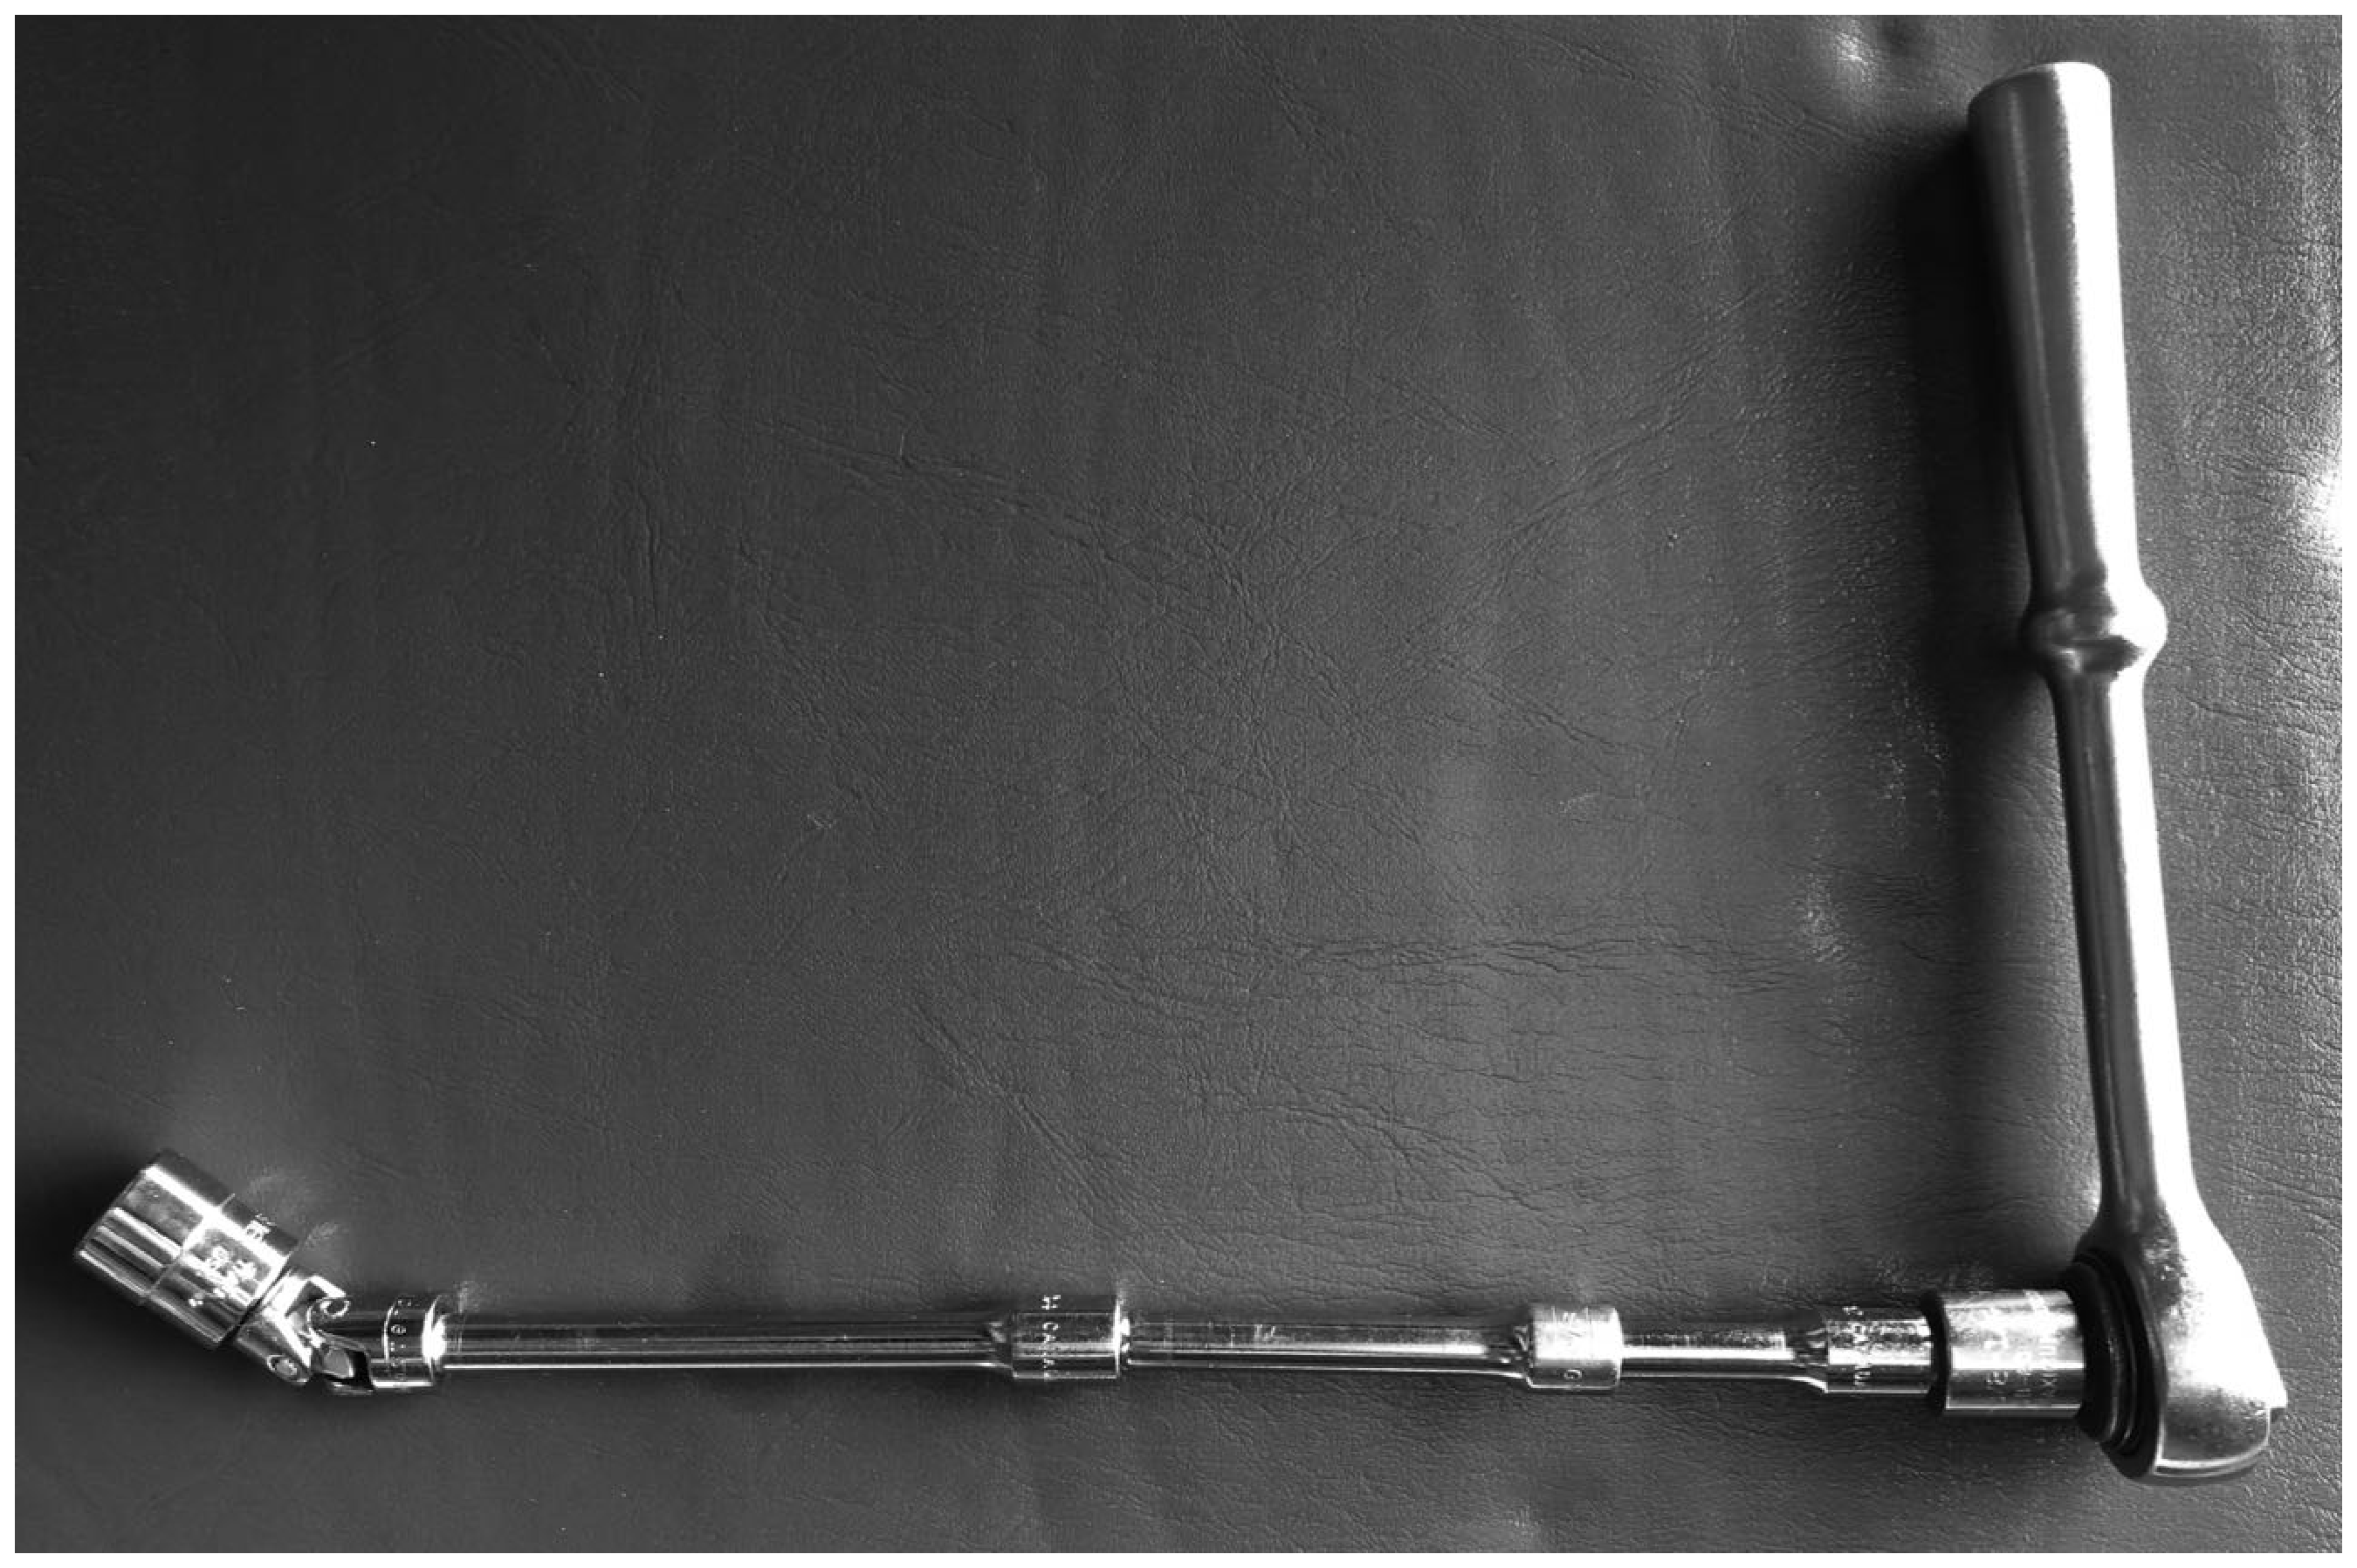
\includegraphics[scale=0.2]{../Diagrams/LG_Box_Fwd}
\end{center}
\caption{Tools for Forward Outboard LG Box Bolts (9/16" Socket)}
\end{figure}

\begin{figure}
[htb]
\begin{center}
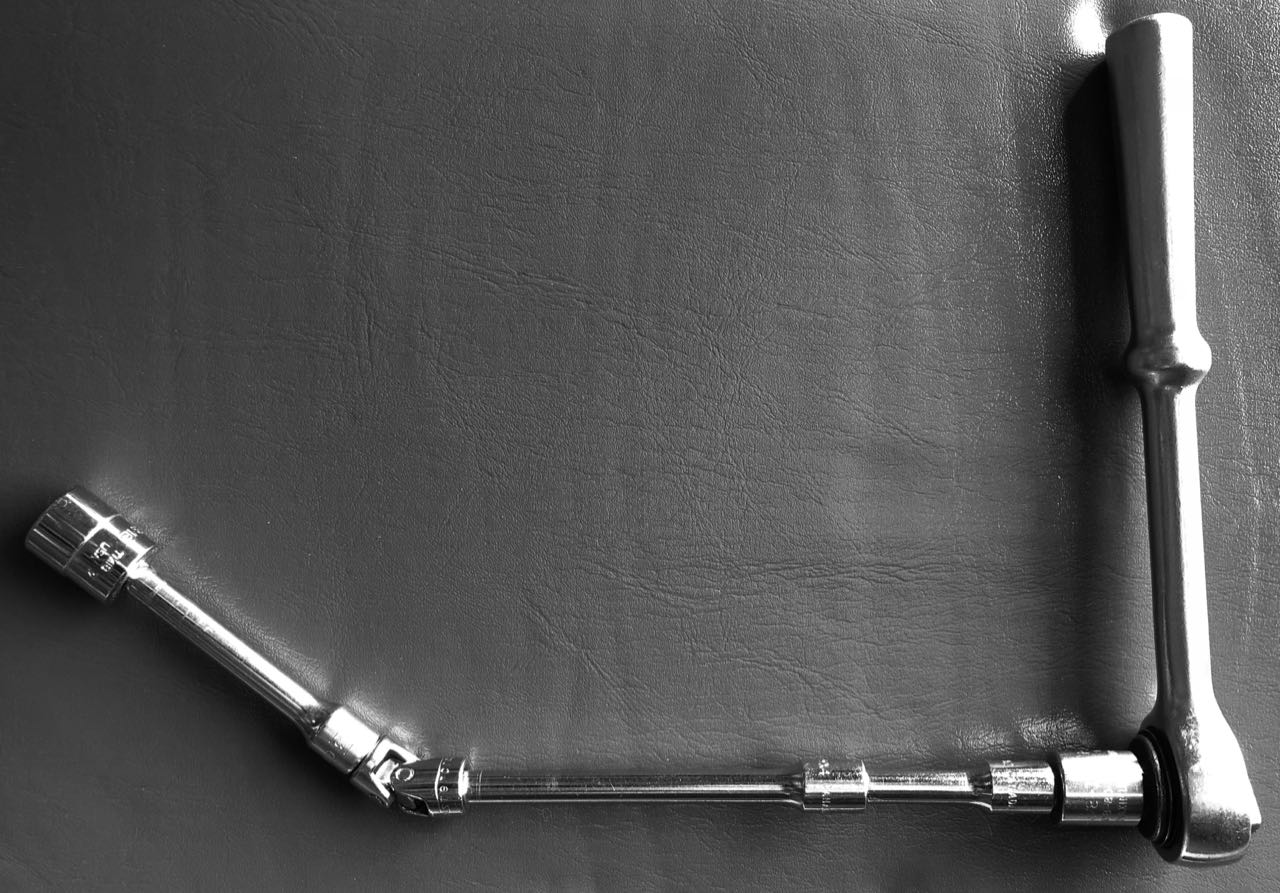
\includegraphics[scale=0.2]{../Diagrams/LG_Box_Aft}
\end{center}
\caption{Tools for Aft Outboard LG Box Bolts (9/16" Socket)}
\end{figure}
      
\clearpage

\section{GNS 430W CONFIGURATION}
\begin{tabularx}{\textwidth} {| >{\setlength\hsize{1.4\hsize}}Y | >{\setlength\hsize{0.8\hsize}}Y | >{\setlength\hsize{0.8\hsize}}Y | c |} 
	\hline Section & Item & Value & Remarks\\
	\hline 
	\hline Main ARINC 429 Config        & IN 1                       & Speed: High         &\\
	                                    &                            & Data: OFF           &\\
	                                    & IN 2                       & Speed: High         &\\
	                                    &                            & Data: OFF           &\\
	                                    & OUT                        & Speed: High         &\\
	                                    &                            & Data: ARINC 429     &\\
	                                    & SDI                        & Common              &\\
	                                    & VNAV                       & Enable Labels       &\\
	\hline Main RSS Config              & Chnl 1                     & Input: Icarus Alt   &from GTX327\\
	                                    &                            & Output: OFF         &\\
	                                    & Chnl 2                     & Input: OFF          &\\
	                                    &                            & Output: ADS-B OUT + &to ADS-B\\
	                                    & Chnl 3                     & Input: OFF          &\\
	                                    &                            & Output: Aviation    &to AFCS and EFIS\\
	                                    & Chnl 4                     & Input: OFF          &\\
	                                    &                            & Output: OFF         &\\
	\hline Main System Config           & Configure                  & Fuel                &\\
	                                    & Fuel Type                  & Av Gas              &\\
	\hline Main System Config           & Configure                  & Discretes           &\\
	                                    & GPS Select                 & Auto                &\\
	                                    & COM Presets                & Enabled             &\\
	\hline COM Setup                    & Spacing                    & 25.0 kHz            &\\
	\hline Main Lighting                & Display Source             & 14V DC              &\\
	                                    & Key Source                 & Photo               &\\
	                                    & Display Resp Time/Min      & 4 / 080             &\\
	                                    & Key Resp Time/Min          & 4 / 40              &\\
	                                    & Display Slope/Offset       & 50 / 50             &\\
	                                    & Key Slope/Offset           & 50 / 50             &\\
	                                    & Key Slope/Offset           & 50 / 50             &\\
	                                    & Display Photo Trans \%     & 05                  &\\
	                                    & Display Photo Slope/Offset & 50 / 50             &\\
	\hline COM Setup                    & S250                       & 15                  &\\
	                                    & S833                       & 20                  &\\
	                                    & Side                       & 31                  &\\
	                                    & Mic                        & 44                  &\\
	\hline VOR/LOC/GS ARINC 429 Config  & Speed                      & RX: Low             &\\
	                                    &                            & TX: Low             &\\
	                                    & SDI                        & VOR/ILS 1           &\\
	                                    & DME Mode                   & Directed Freq 1     &\\
	\hline GPS Vertical Offset          & GPS Antenna Height         & 4 ft                &\\
	\hline 
\end{tabularx}
\clearpage


\section{uAVIONICS EchoUAT ADS-B CONFIGURATION}
\begin{tabularx}{\textwidth} {| >{\setlength\hsize{1.1\hsize}}Y | >{\setlength\hsize{1.1\hsize}}Y | >{\setlength\hsize{0.8\hsize}}Y | c |} 
	\hline Section & Item & Value & Remarks\\
	\hline 
	\hline Transceiver Config           & Control                                        & UAT TX Enabled       &\\
	                                    & ICAO Number                                    & C067BD               &\\
	                                    & Call Sign                                      & CGNHK                &\\
	                                    & Flight Plan ID                                 & left blank           &\\
	                                    & CSID Logic                                     & Enabled              &\\
	                                    & Anonymous Mode                                 & Disabled             &\\
	                                    & Emitter Category                               & Light Airplane       &\\
	                                    & VFR Code                                       & 1200                 &\\
	                                    & ADS-B IN Capability                            & Both 1090/978 MHz    &\\
	                                    & VSO                                            & 40                   &\\
	                                    & Aircraft Length (m)                            & L$\leq$15            &\\
	                                    & Aircraft Width (m)                             & W$\leq$23            &\\
	                                    & GPS Antenna Offset Lateral (m)                 & 0                    &\\
	                                    & GPS Ant Offset from nose (m)                   & 4                    &\\
	\hline Installation                 & Setup Source                                   & App (WiFi) Stored    &\\
	                                    & Control Source                                 & Transponder Monitor  &\\
	                                    & GPS Source                                     & External GPS (COM 2) &\\
	                                    & Traffic Uplink Output                          & MFD (COM 2)          &Not Connected\\
	                                    & COM 1 Rate                                     & 38400                &Not Connected\\
	                                    & COM 1 Data                                     & 810                  &Not Connected\\
	                                    & COM 1 Phy                                      & RS-485 Terminated    &Not Connected\\
	                                    & COM 1 Protocol                                 & TMAP                 &Not Connected\\
	                                    & COM 2 Rate                                     & 9600                 &\\
	                                    & COM 2 Input Protocol                           & ADS-B+               &\\
	\hline Advanced                     & Transponder Threshold                          & 1450                 &Reduced from default\\
	(Double Tap 'echo' at               &                                                &                      &value of 1550 to\\
	top of Echo iOS App                 &                                                &                      &improve Pressure\\
	to see Advanced options)            &                                                &                      &Altitude detection\\
	\hline 
\end{tabularx}
\clearpage

\section{GARMIN GTX-327 CONFIGURATION}
\begin{tabularx}{\textwidth} {| >{\setlength\hsize{1.1\hsize}}Y | >{\setlength\hsize{1.1\hsize}}Y | >{\setlength\hsize{0.8\hsize}}Y | c |} 
	\hline Section & Item & Value & Remarks\\
	\hline 
	\hline Display Mode                 & Display Mode                                   & AUTO                 &\\
	                                    & Level                                          & 85                   &\\
	\hline Backlight                    & BKLT                                           & MAN                  &\\
	                                    & LVL                                            & ----                 &Current Value\\
	                                    & RSP TIME                                       & 1                    &\\
	                                    & MIN                                            & 10                   &\\
	                                    & BKLT SRCE                                      & PHOTO                &\\
	                                    & SLOPE                                          & 50                   &\\
	                                    & OFFSET                                         & 50                   &\\
	\hline Key Lighting                 & KEY                                            & AUTO                 &\\
	                                    & LVL                                            & ----                 &Current Value\\
	                                    & RSP TIME                                       & 1                    &\\
	                                    & MIN                                            & 10                   &\\
	                                    & KEY SRCE                                       & PHOTO                &\\
	                                    & SLOPE                                          & 50                   &\\
	                                    & OFFSET                                         & 50                   &\\
	\hline 
\end{tabularx}

\section{TRIO PRO PILOT AUTOPILOT CONFIGURATION}
\begin{tabularx}{\textwidth} {| >{\setlength\hsize{1.1\hsize}}Y | >{\setlength\hsize{1.1\hsize}}Y | >{\setlength\hsize{0.8\hsize}}Y | c |} 
	\hline Section & Item & Value & Remarks\\
	\hline 
	\hline Config Settings              & HNAV Servo Position                            & 7916                 &\\
	                                    & HNAV Servo Direction                           & NM                   &\\
	                                    & VNAV Servo Direction                           & RV                   &\\
	                                    & AS/VS Select                                   & AS                   &\\
	                                    & Max Turn Rate                                  & Auto                 &\\
	                                    & Circle Last Waypoint                           & No                   &\\
	                                    & Default Vertical Rate                          & 500                  &\\
	                                    & AP Disconnect Mode                             & HNAV \& VNAV         &\\
	                                    & LED Flash Mode                                 & Fast Flash           &\\
	                                    & Zero Flight Data on Power Up                   & No                   &\\
	\hline Autopilot Preferences        & Backlight                                      & 9                    &\\
	                                    & Contrast                                       & (Blank)              &\\
	                                    & HNAV TRK Gain                                  & 3                    &\\
	                                    & HNAV CRS Gain                                  & 4                    &\\
	                                    & HNAV PI Gain                                   & 9                    &\\
	                                    & HNAV Servo Gain                                & 35                   &\\
	                                    & VNAV Servo Gain                                & 16                   &\\
	                                    & VNAV AH Gain                                   & 60                   &\\
	                                    & VNAV VS Gain                                   & 50                   &\\
	                                    & VNAV AS Gain                                   & 35                   &\\
	                                    & VNAV Servo Deadband                            & 4                    &\\
	\hline 
\end{tabularx}


\clearpage

\section{TORQUE TABLE} 
\begin{tabularx}
	{
	\textwidth}{|>{\setlength\hsize{.9\hsize}}Y|c|>{\setlength\hsize{1.1\hsize}}Y|} \hline Item&Torque Value&Remarks\\
	\hline \hline Main Alternator Mount&110 -- 150 in-lb&from Installation Instructions\\
	\hline Main Alternator Tension Arm&110 -- 150 in-lb&from Installation Instructions\\
	\hline Main Alternator Pivot Bolt&30 -- 40 ft-lb&from Installation Instructions\\
	\hline \ifthenelse{\thePMAG = 0}{Spark Plugs (Aviation)&35 ft-lb&from Lycoming Overhaul Manual\\
	\hline Spark Plugs (Automotive)&180 in-lb&from Electronic Ignition Installation Instructions\\}	
	{Spark Plugs&180 in-lb&from PMag and Electronic Ignition Installation Instructions\\}
	\hline \ifthenelse{\thePMAG = 1}{PMag Spark Plug Adapters&18 ft-lb&Screw adapters onto sparkplugs, and torque via the spark plug. Do no apply anti-seize. from PMag Installation Instructions\\
	\hline Light Speed Spark Plug Adapters&25 ft-lb&Do not apply anti-seize. from Electronic Ignition Installation Instructions\\}
	{\hline Light Speed Spark Plug Adapters&25 ft-lb&Do not apply anti-seize. from Electronic Ignition Installation Instructions\\}
	\hline Rocker Box Screws&50 in-lb&from Lycoming Overhaul Manual\\
	\hline Intake pipe bolts with silicone gaskets&15 in-lb&from Steve Mahoney\\
	\hline Exhaust Pipe Nuts&180 -- 200 in-lb&Apply anti-seize. from Vetterman Exhaust Installation Instructions\\
	\hline \ifthenelse{\thePMAG = 0}{Magneto}{PMag} and EI Hall Effect Unit Base Clamps&204 in-lb&from ECI Service Info\\
	\hline Propeller Governor Mounting Nuts&110 -- 150 in-lb&from PCU-5000 Installation and Adjustment document\\
	\hline Propeller Governor High RPM Stop Jam Nut&24.8 -- 28.3 in-lb&from PCU-5000 Installation and Adjustment document\\
	\hline Oil Screen&135\textdegree \ rotation after contact&from Lycoming SSP-1776-B\\
	\hline Propeller Hub&63 -- 66 ft-lb&from MT Operation and Installation manual\\
	\hline Spinner Screws&35 -- 44 in-lb&from MT Operation and Installation manual\\
	\hline Brake caliper bolts&75 -- 80 in-lb&from Cleveland service info\\
	\hline Wheel half bolts&90 in-lb&Bolts that join the two halves of each wheel. Value from Cleveland service info\\
	\hline Landing gear outboard 7/16" bolts&240 in-lb&from RV-8 Builder's Manual\\
	\hline Landing gear inboard 7/16" bolts&450 -- 500 in-lb&from AC43.13-1B\\
	\hline Landing gear inboard 5/16" bolts&100 -- 140 in-lb&from AC43.13-1B\\
	\hline 
\end{tabularx}

\clearpage
\section{FUSE BLOCKS}
\begin{figure}
  \centering
  % 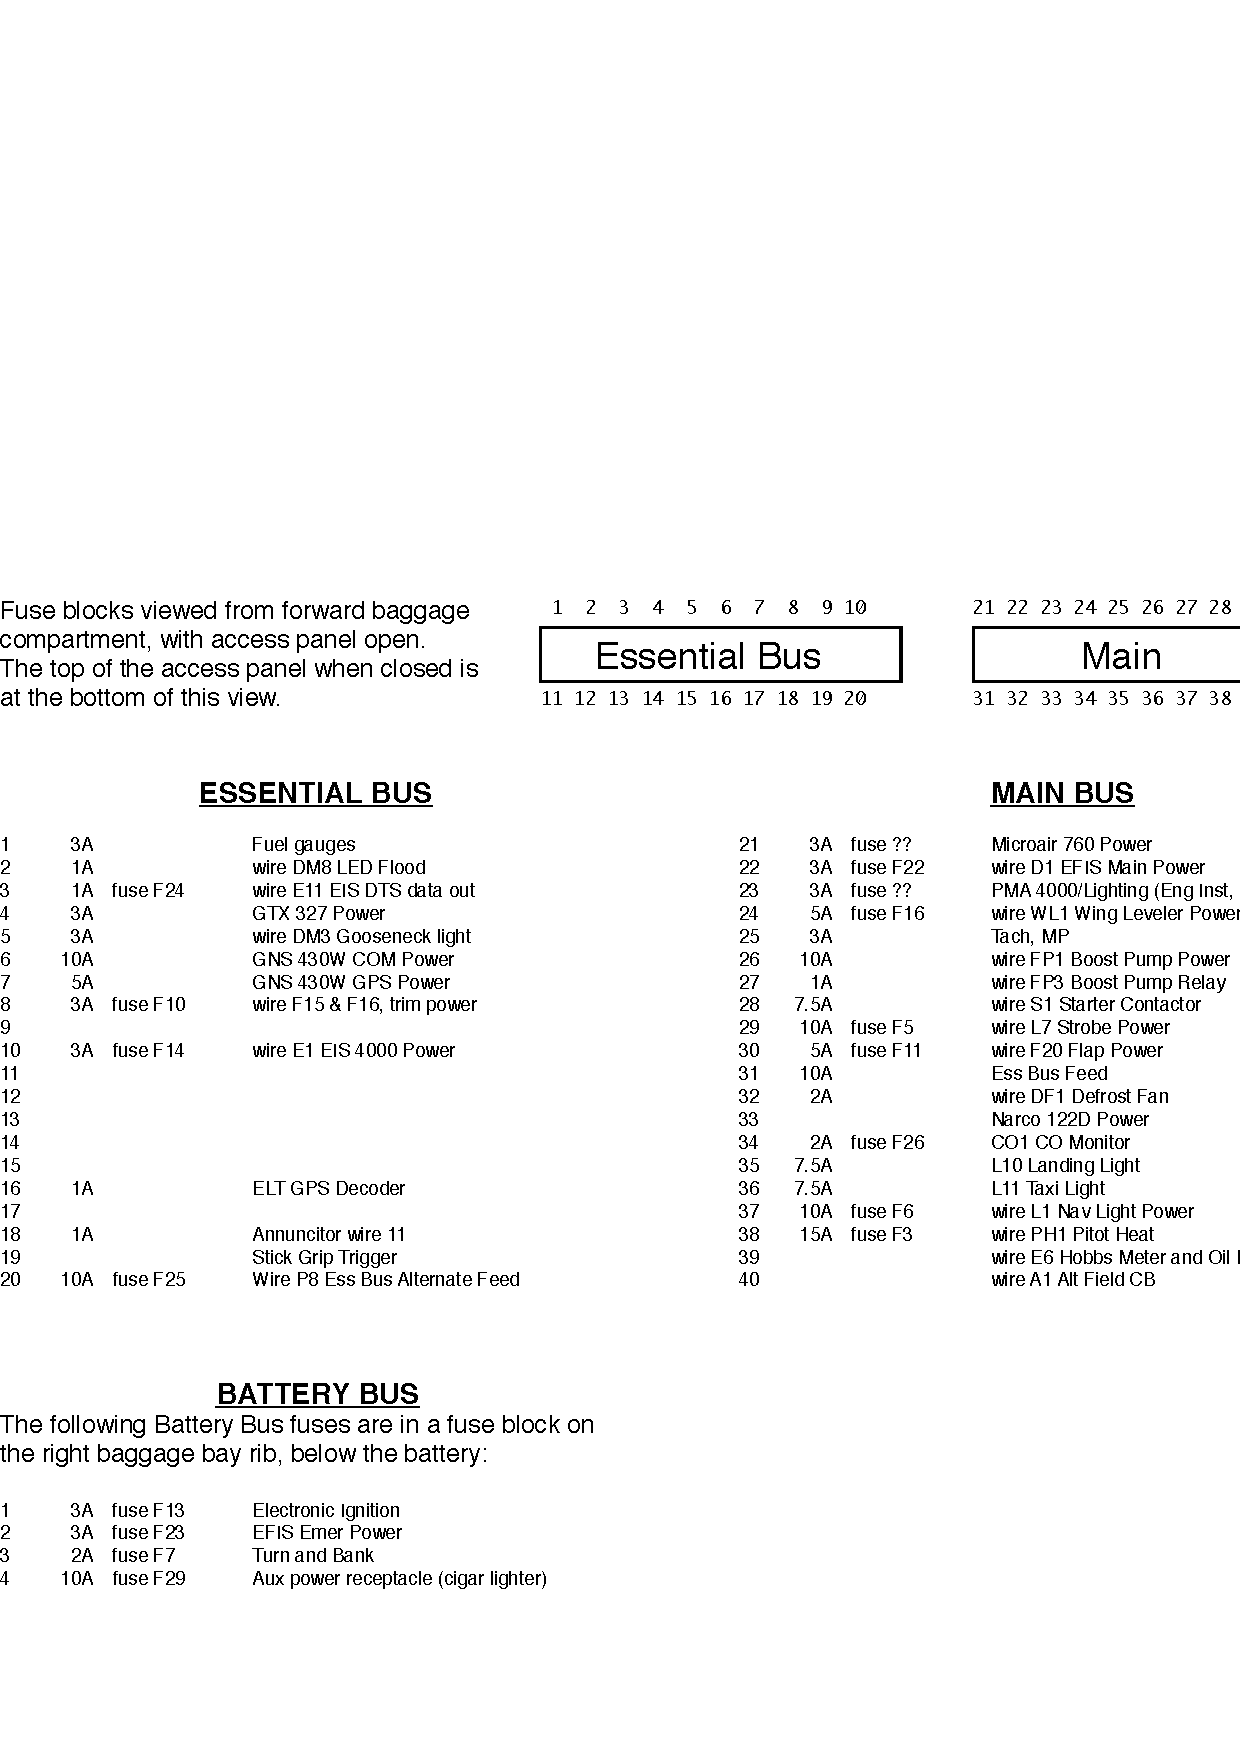
\includegraphics[width=1.1\textwidth, angle=90]{../Diagrams/Fuse_Blocks_POH}
  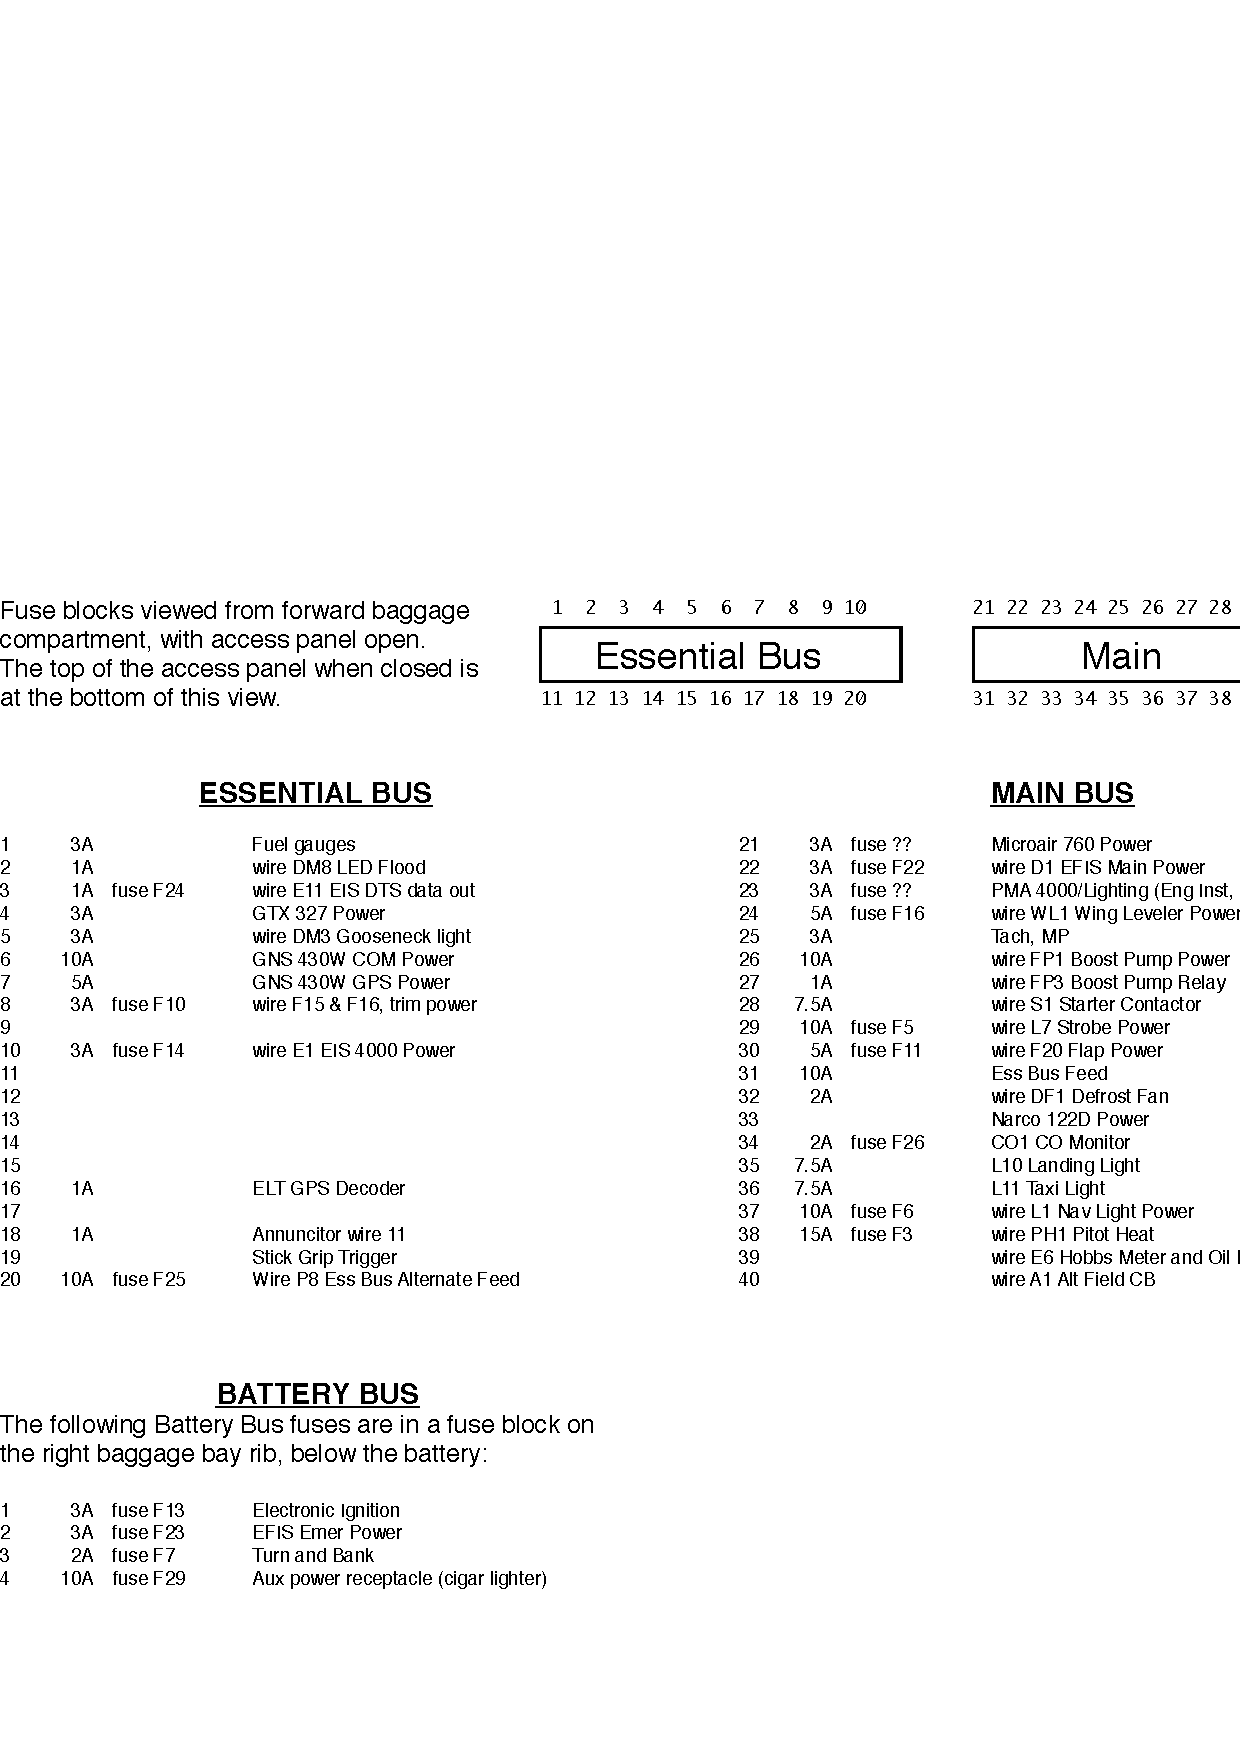
\includegraphics[width=1.2\textwidth, angle=90]{../Diagrams/Fuse_Blocks_POH}
  \label{fig:FuseBlocks}
  \caption{Fuse Blocks}
\end{figure}
\cleardoublepage 

\chapter{EQUIPMENT LIST}
\vspace{\minitocspacebefore}
\minitoc
\cleardoublepage

% \section{INTRODUCTION}
% \textcolor{red}{This is a place-holder for the list of installed equipment.  It will be completed with a list of manufacturers, part numbers and serial numbers of the installed equipment and miscellaneous parts.}

% \textcolor{red}{Rework the table formats to get the same column width in all tables.}

% !iTeXMac(input): POH.tex
% \chapter{EQUIPMENT LIST}
% \vspace{\minitocspacebefore}
% \minitoc
% \cleardoublepage
% 
% \section{INTRODUCTION}
% % \textcolor{red}{This is a place-holder for the list of installed equipment.  It will be completed with a list of manufacturers, part numbers and serial numbers of the installed equipment and miscellaneous parts.}
% 
% % \textcolor{red}{Rework the table formats to get the same column width in all tables.}

\section{ENGINE}
\begin{tabularx}{\textwidth}{|>{\setlength\hsize{.9\hsize}}Y|c|c|c|>{\setlength\hsize{1.1\hsize}}Y|}
  \hline
  Item&Manufacturer&Part No.&Serial No.&Remarks\\
  \hline
  \hline
  Engine&Lycoming&IO-360-A1B6&L-25562-51A&Overhauled by Aerosport Power\\
  \hline
  Propeller&MT&MTV-12-B-C/C183-59B&?&72" diameter. Blade SN ?\\
  \hline
  Propeller Governor&Aero Technologies&PCU-5000X P-540-036/A-866&08401955&Purchased from American Propeller. Gasket PN MS9144-01\\
  \hline
  Oil Cooler&Stewart Warner&10599R&&or Aero-Classics HE 8001599\\
  \hline
\ifthenelse{\thePMAG = 0}{Magneto&Slick&4371 rev C&98112422&\\}{Electronic Ignition&E-Mag&P-114&&\\}
  \hline
  Electronic Ignition&Light Speed Engineering&Plasma II&31762&\\
  \hline
  Spark Plugs (Top)&Denso&W27ESR-U&-&\\
  &or&&&\\
  &NGK&BR9ES&-&\\
  \hline
\ifthenelse{\thePMAG = 0}
  {Spark Plugs (Bottom)&Tempest(Autolite)&URHM38E&-&Massive Electrode\\
  &or&&&\\
  &Tempest&URHM38S&-&Fine Wire Electrode\\}
  {Spark Plugs (Bottom)&Denso&W24ESR-U&-&\\
  &or&&&\\
  &NGK&BR8ES&-&\\}
  \hline
  Air Filter&K\&N&33-2060&-&Van's PN E 33-2060\\
  \hline
  Oil Filter&Champion&CH48110-1&-&\\
  &Tempest&AA48110-2&-&\\
  \hline
  Throttle Cable&Tuthill - Cablecraft&184 VTT-2-60&-&Van's PN CT Q-60\\
  \hline
  Mixture Cable&Tuthill - Cablecraft&184 VTT-2-52&-&from Van's. Custom length.  52"\\
  \hline
  Prop Control Cable&Tuthill - Cablecraft&184 VTT-2-48&-&Van's PN CT Q-48\\
  \hline
  Alternate Air Control Cable&ACS Products&A-740BL0720&-&\\
  \hline
  Oil Cooler Door Control Cable&ACS Products&A-820BL0360&-&\\
  \hline
  Heater Box Cable (Front Seat)&ACS Products&A-740BL0720&-&\\
  \hline
  Heater Box Cable (Rear Seat)&ACS Products&A-740BL0720&-&\\
  \hline
  \end{tabularx}
  
\section{ENGINE INSTRUMENTS}
\begin{tabularx}{\textwidth}{|>{\setlength\hsize{.9\hsize}}Y|c|c|c|>{\setlength\hsize{1.1\hsize}}Y|}
  \hline
  Item&Manufacturer&Part No.&Serial No.&Remarks\\
  \hline
  \hline
   Engine Monitor&Grand Rapids&EIS 4000&20683-A&SW Vers 44S81F\\
   \hline
   Tachometer&Van's Aircraft&IE VTACCH3500&-&\\
  \hline
   Tach Extension Cable&Van's Aircraft&IE VTACH EXT12&-&\\
  \hline
   Tach Transducer&Van's Aircraft&IE VTACH GEN12&-&\\
  \hline
   Manifold Pressure Gauge&Van's Aircraft&IE VMP35&-&\\
  \hline
   Fuel Gauges&Van's Aircraft&IE VFL15&-&Van's Aircraft PN\\
  \hline
   Fuel Gauge Senders&Van's Aircraft&IE F-385B (L tank) IE F-385C (R tank)&-&\\
  \hline
   Fuel Pressure Transducer&VDO&360 003&-&from Young's Speed Shop, Ottawa.  80 psi sender, 10 - 180 ohms\\
  \hline
   Oil Pressure Transducer&VDO&360 004&-&150 psi sender, 10 - 180 ohms\\
  \hline
   Oil Pressure Switch&Datcon&100451&-&15 psi switch\\
   \hline
   Hourmeter&Hobbs&85000 Series&&ACS P/N 15000\\
   \hline
  \end{tabularx}

\section{FLIGHT INSTRUMENTS}
\begin{tabularx}{\textwidth}{|>{\setlength\hsize{.9\hsize}}Y|c|c|c|>{\setlength\hsize{1.1\hsize}}Y|}
  \hline
  Item&Manufacturer&Part No.&Serial No.&Remarks\\
  \hline
  \hline
  EFIS&Dynon Avionics&100321- Rev 0&004439&Model D10A\\
  \hline
  ASI&UMA&16-311-241&C2587&\\
  \hline
  Altimeter&United Instruments&5934PD-3&400700&TSO'd\\
  \hline
  VSI&Falcon Wultrad&VSI4FM-3&VSIE0206004&Made in China\\
  \hline
  Turn and Bank&Electric Gyro Corp&1234T100-7TZ&2310-176&\\
  \hline
  Compass&&MC021&052&Made in China\\
  \hline
  Annunciators&Aerospace Optics Inc.&32245-99-530&&Mil Std M22885/90 Vivisun 20/20\\
  \hline
  Pitot Tube&Aero Instrument Co.&PH 502-12&&AN5812-12\\
  \hline
  \end{tabularx}

\section{ELECTRICAL SYSTEM}
\begin{tabularx}{\textwidth}{|>{\setlength\hsize{.9\hsize}}Y|c|c|c|>{\setlength\hsize{1.1\hsize}}Y|}
  \hline
  Item&Manufacturer&Part No.&Serial No.&Remarks\\
  \hline
  \hline
  Battery&Odyssey&PC680&-&\\
  \hline
  Main Alternator&B\&C Specialty Products&L-60&-&Boss mount.\\
  \hline
  Alternator Belt&Gates&7365 (11A0925)&-&3/8" x   37 1/8"\\
  \hline
  Standby Alternator&B\&C Specialty Products&SD-8&\textcolor{red}{??}&\\
  \hline
  Starter&SkyTec&149-12LS&\textcolor{red}{??}&Solenoid on starter from 2005 Ford Crown Victoria\\
  \hline
  Battery Contactor&\textcolor{red}{??}&\textcolor{red}{??}&-&\\
  \hline
  Starter Contactor&\textcolor{red}{??}&\textcolor{red}{??}&-&\\
  \hline
  Essential Bus Diode&\textcolor{red}{??}&\textcolor{red}{??}&-&\\
  \hline
  Alternator Field CB&Klixon&7274-11-5 &-&MS22073-5 5A CB\\
  \hline
  Standby Alternator CB&Klixon&7274-11-5 &-&MS22073-5 5A CB\\
  \hline
  Alternator Current Limiter (80a)&Cooper Bussman&ANL-80&-&B\&C Specialty Products C905-80\\
  \hline
  \end{tabularx}
  
\section{LIGHTING}
     \begin{tabularx}{\textwidth}{|>{\setlength\hsize{.9\hsize}}Y|c|c|c|>{\setlength\hsize{1.1\hsize}}Y|}
       \hline   
       Item&Manufacturer&Part No.&Serial No.&Remarks\\
       \hline
       \hline
       Landing \& Taxi Lights&-& - &-&\\
       \hline
       Instrument Panel Flood Lights&-&-& - &\\
       \hline
       Annunciator Lamp Bulb&MRO&56-0022-2& - &T1 Midget flange bulb from MRO, Calgary, 1-800-882-9301Fa1b6\\
       \hline
       \end{tabularx}

\section{COCKPIT}
  \begin{tabularx}{\textwidth}{|>{\setlength\hsize{.9\hsize}}Y|c|c|c|>{\setlength\hsize{1.1\hsize}}Y|}
    \hline   
    Item&Manufacturer&Part No.&Serial No.&Remarks\\
    \hline
    \hline
    Defrost Fan&Mode Electronics&59-294-0& - &from Gervais Electronics, Ottawa\\
    \hline
    Defrost Fan Grill Guard&Mode Electronics&59-319-0& - &from Gervais Electronics, Ottawa\\
    \hline
    \end{tabularx}

\section{AVIONICS}
  \begin{tabularx}{\textwidth}{|>{\setlength\hsize{.9\hsize}}Y|c|c|c|>{\setlength\hsize{1.1\hsize}}Y|}
    \hline
    Item&Manufacturer&Part No.&Serial No.&Remarks\\
    \hline
    \hline
    GPS&Garmin&011-01060-40&97108744&GNS 430W, mod level 5\\
    \hline
    Transponder&Garmin&011-00490-00&83710639&GTX 327, mod level 0\\
    \hline
    Nav 2&Narco&Nav 122D&10499&Warranty \#031280300.  Narco ship date 10 Mar 05.  Dealer code 27025\\
    \hline
    Com 2&Microair&760&M760-005772&\\
    \hline
    CDI&Mid Continent Instruments&MD200-306&E22527&\\
    \hline
    GPS Antenna&Garmin&GA 35&25136&manufactured by AeroAntenna Technology as P/N AT575-93GW-TNCF-000-RG-27-NM\\
    \hline
    Com 1 Antenna&Comant Industries&CI-122&-&\\
    \hline
    Com 2 Antenna&Sportcraft&SA-001A-1&&Left wing tip\\
    \hline
    Nav Antenna&Sportcraft&SA-001-1&&Right wing tip\\
    \hline
    Nav Antenna Splitter&Comant Industries&CI 1125&4085047&\\
    \hline
    ELT&ACK&E-04&001510&Hex ID: 27878 0CF7A FFBFF Aircraft Address: 12609469. 24 bit ICAO Address: C067BD\\
    \hline
    Altitude Encoder&Trans-Cal&SSD120-30N&18879&\\
    \hline
    Intercom&PS Engineering&1194 0&BM-01352&PMA4000\\
    \hline
    Autopilot&Trio Avionics&Pro Pilot&PPR0316VL&SW version OP120710\\
    \hline
    Autopilot Pitch Servo&Trio Avionics&Gold Standard Servo&S4091&\\
    \hline
    Autopilot Roll Servo&Navaid Devices&S-2&1444&\\
    \hline
    CO Monitor&CO Guardian&252&AE6094&\\
    \hline
    Remote Flux Valve&Dynon&100323- Rev 0&003899&Model EDC-D10A\\
    \hline
    \end{tabularx}


\section{FLIGHT CONTROLS}
  \begin{tabularx}{\textwidth}{|>{\setlength\hsize{.9\hsize}}Y|c|c|c|>{\setlength\hsize{1.1\hsize}}Y|}
    \hline
    Item&Manufacturer&Part No.&Serial No.&Remarks\\
    \hline
    \hline
    Trim/AFCS disconnect relay&NTE&R14-11D10-12& - &from Active Electronics, Ottawa\\
    \hline
    Trim/AFCS disconnect relay socket&NTE&R95-111& - &from Gervais Electronics, Ottawa\\
    \hline
    \end{tabularx}




\section{MISC}
\begin{tabularx}{\textwidth}{|>{\setlength\hsize{.9\hsize}}Y|c|c|c|>{\setlength\hsize{1.1\hsize}}Y|}
       \hline   
       Item&Manufacturer&Part No.&Serial No.&Remarks\\
       \hline
       \hline
       Baggage Door and Canopy Locks&ACS&11-01600&&Key \# ACS256\\
       \hline
       Wheel Assembly&Cleveland&40-78B&&5" Wheel\\
       \hline
       Brake Disc&Cleveland&164-01700&&\\
       \hline
       Brake Assembly&Cleveland&30-9&&\\
       \hline
       Brake Lining&Cleveland&066-10600&&Part No. is for lining only. Must be riveted to backing plates with 105-00200 rivets.\\
       \hline
       Fuel Tank Quick Drain Valve&SAF AIR&CAV-110&&\\
       \hline
       Fuel Tank Quick Drain Valve O-Ring&&MS29513-006&&Replacement O-ring for SAF-AIR CAV-110 drain valve.\\
       \hline
       \end{tabularx}

  % \cleardoublepage


\end{document}
